\documentclass[12pt,a4paper]{article}
\usepackage[utf8]{inputenc}
\usepackage[spanish,es-tabla]{babel}
\usepackage{graphicx}
\usepackage{listings}
\usepackage{hyperref}
\usepackage{geometry}
\usepackage{float}
\usepackage{caption}
\usepackage{tabularx}
\usepackage{booktabs}
\usepackage{amsmath}
\usepackage[table,xcdraw]{xcolor}
\usepackage{titlesec}
\usepackage{fancyhdr}
\usepackage{enumitem}
\usepackage{tcolorbox}
\usepackage{tikz}
\usepackage{xltabular}
\usepackage{lscape}
\usetikzlibrary{shapes.geometric, arrows.meta, positioning}

% =======================================================================
% CONFIGURACIÓN DE PALETA DE COLORES EJECUTIVA
% =======================================================================
\definecolor{NavyPrimary}{RGB}{20, 45, 85}
\definecolor{SlateSecondary}{RGB}{70, 80, 95}
\definecolor{AccentBlue}{RGB}{0, 114, 206}
\definecolor{LightGrayBG}{RGB}{248, 249, 252}
\definecolor{BorderGray}{RGB}{218, 222, 230}
\definecolor{DarkText}{RGB}{30, 35, 45}

% =======================================================================
% CONFIGURACIÓN DE PÁGINA Y MARGENES
% =======================================================================
\geometry{top=2.5cm, bottom=2.5cm, left=2.5cm, right=2.5cm}
\linespread{1.15}

\usepackage{helvet}
\renewcommand{\familydefault}{\sfdefault}

\graphicspath{{Entregable 4/}{Entregable 3/}{Entregable 2/}{./}}

% =======================================================================
% ESTILO DE ENCABEZADOS Y PIE DE PÁGINA
% =======================================================================
\setlength{\headheight}{14pt}
\pagestyle{fancy}
\fancyhf{}
\lhead{\small\color{SlateSecondary}\textbf{ARQ-WEB 2026} -- Proyecto Integrador}
\rhead{\small\color{SlateSecondary}Despliegue y Aseguramiento de BookStack}
\lfoot{\small\color{SlateSecondary}FP-UNA -- Facultad Politécnica}
\rfoot{\small\color{NavyPrimary}\textbf{\thepage}}
\renewcommand{\headrulewidth}{0.5pt}
\renewcommand{\footrulewidth}{0.4pt}

% =======================================================================
% FORMATO DE TÍTULOS Y SECCIONES
% =======================================================================
\titleformat{\section}
  {\color{NavyPrimary}\sffamily\Large\bfseries}
  {\thesection.}{0.5em}{}[\color{NavyPrimary}\titlerule]

\titleformat{\subsection}
  {\color{NavyPrimary}\sffamily\large\bfseries}
  {\thesubsection.}{0.5em}{}

\titleformat{\subsubsection}
  {\color{SlateSecondary}\sffamily\normalsize\bfseries}
  {\thesubsubsection.}{0.5em}{}

% =======================================================================
% CONFIGURACIÓN DE CAJAS LIGERAS (TCOLORBOX)
% =======================================================================
\newtcolorbox{adrbox}[1]{
  colback=LightGrayBG,
  colframe=NavyPrimary,
  coltitle=white,
  fonttitle=\bfseries\sffamily\small,
  title={#1},
  arc=3pt,
  boxrule=0.8pt,
  top=6pt, bottom=6pt, left=8pt, right=8pt
}

% =======================================================================
% CAPTIONS Y HIPERVÍNCULOS
% =======================================================================
\captionsetup{font=small,labelfont={bf,color=NavyPrimary},labelsep=colon}

\hypersetup{
    colorlinks=true,
    linkcolor=NavyPrimary,
    filecolor=AccentBlue,      
    urlcolor=AccentBlue,
    citecolor=NavyPrimary,
    pdftitle={Trabajo Práctico Integrador I y II -- ARQ-WEB 2026},
}

% =======================================================================
% INICIO DEL DOCUMENTO
% =======================================================================
\begin{document}

\begin{center}
    {\color{NavyPrimary}\Huge\bfseries Trabajo Práctico Integrador I y II}\\[0.3cm]
    {\color{SlateSecondary}\Large\bfseries Asignatura: Arquitectura Web -- FP-UNA 2026}\\[0.5cm]
    {\color{DarkText}\large\textbf{Despliegue, conectividad, seguridad TLS 1.3, verificación experimental, resiliencia y observabilidad de una aplicación web}}\\[0.6cm]
    
    \begin{tcolorbox}[colback=LightGrayBG,colframe=BorderGray,arc=3pt,boxrule=0.5pt,width=0.95\textwidth]
        \centering \small
        \textbf{Autores:} Sofia Mereles \quad|\quad Alba Martinez \quad|\quad Guillermo Gonzalez\\
        \textbf{Institución:} Facultad Politécnica -- Universidad Nacional de Asunción (FP-UNA)\\
        \textbf{Fecha:} Noviembre 2026 -- Diseño de Fase 5 A1--A5
    \end{tcolorbox}
\end{center}

\vspace{0.2cm}

\begin{abstract}
\noindent El presente informe documenta las Fases 1, 2, 3 y 4 del proyecto integrador de la asignatura \textbf{Arquitectura Web}. En la primera etapa se estableció la línea base de la infraestructura servidor mediante la configuración de un entorno virtualizado en Ubuntu Server en modo puente (\textit{Bridged}), evaluando y seleccionando la plataforma \textbf{BookStack}. En la segunda etapa se llevó a cabo el despliegue del stack LNMP (Linux, Nginx, MariaDB, PHP 8.5-FPM), la ejecución de migraciones de base de datos y la verificación del servicio HTTP. En la tercera etapa se implementó la capa de seguridad con TLS 1.3 sobre el dominio \texttt{bookstack.local}, la redirección automática HTTPS, la evaluación experimental del rendimiento de la negociación criptográfica, la inspección de cabeceras HTTP/Gzip/Caché, la comparativa de arquitectura entre proxy e interfaz FastCGI, y el análisis de trazas de red mediante \texttt{tcpdump}. Finalmente, en la cuarta etapa se realizó el endurecimiento (\textit{hardening}) del firewall UFW, la auditoría avanzada de cabeceras de seguridad, la simulación de fallos y resiliencia de servicios, pruebas de carga concurrente con \texttt{ab}, la observabilidad en tiempo real con \texttt{htop} y la matriz de pruebas consolidada.
\end{abstract}

\noindent\textbf{Continuación del TP II.} Se incorpora el análisis A1 de la
Fase 5, con inventario del esquema real, matriz de acoplamiento respaldada
por código y mapas de contextos del monolito y de su integración. El análisis documenta
los seis módulos funcionales y las evidencias F5-E1 a F5-E3. Se incorporan
también los ADR-006 a ADR-010 del apartado A2, con decisiones, alternativas
y consecuencias para la evolución de la plataforma. El apartado A3 define
los contratos HTTP y de eventos, su política de versionado y la validación
reproducible F5-E4. A4 incorpora el modelo C4 de contexto y contenedores,
las tres secuencias obligatorias con caminos de error y las evidencias F5-E5 a F5-E7.
A5 completa el diseño con el plan de migración, los criterios de hecho,
la reversión planificada y la matriz de riesgos.

\vspace{0.2cm}
\tableofcontents
\newpage

% =======================================================================
% SECCIÓN 1: OBJETIVOS, ALCANCE Y CRITERIOS
% =======================================================================
\section{Objetivos, Alcance y Criterios de Aceptación}
El objetivo general del proyecto es diseñar, desplegar y auditar una infraestructura servidor segura, resiliente y observable, ejecutando sobre ella la aplicación web de gestión del conocimiento \textbf{BookStack}.

\begin{itemize}[leftmargin=1.5em, itemsep=3pt]
    \item \textbf{Alcance (Fase 1):} Preparación de la máquina virtual (2 vCPU, 4 GB RAM, 20 GB Disco), asignación de direccionamiento IP en capa 3, habilitación de OpenSSH, verificación de conectividad ICMP bidireccional y definición de la arquitectura lógica de tres capas.
    \item \textbf{Alcance (Fase 2):} Despliegue del stack LNMP; creación del esquema relacional en MariaDB; ejecución de migraciones de Laravel/BookStack; configuración del servidor virtual en Nginx y validación del flujo HTTP.
    \item \textbf{Alcance (Fase 3):} Configuración de resolución de nombres local (\texttt{bookstack.local}); generación e inspección de certificado digital X.509 con SAN; habilitación de HTTPS (TLS 1.3) con redirección 301; evaluación experimental de latencia con \texttt{curl}; auditoría de compresión Gzip y caché (304 Not Modified); comparativa técnica de arquitectura y análisis de traza de red con \texttt{tcpdump}.
    \item \textbf{Alcance (Fase 4):} Restricción de superficie de ataque mediante firewall UFW; auditoría de cabeceras de seguridad HTTP y atributos de cookies (\texttt{Secure}, \texttt{HttpOnly}, \texttt{SameSite}); validación de resiliencia ante caída del backend (HTTP 502) y autoarranque tras reinicio; pruebas de carga concurrente con \texttt{ab}; monitoreo de recursos en vivo (\texttt{htop}) y consolidación de evidencias.
    \item \textbf{Criterios de Aceptación:} Comunicación ICMP sin pérdida de paquetes, protocolo TLS 1.3 activo en puerto 443/TCP, redirección permanente HTTP 301 desde el puerto 80/TCP, cookies de sesión marcadas como \texttt{Secure} e \texttt{HttpOnly}, 0\% de fallos en pruebas de carga concurrente de 1.000 peticiones, y autoarranque verificado de todos los demonios del sistema tras un reinicio físico de la VM.
\end{itemize}

% =======================================================================
% SECCIÓN 2: SELECCIÓN DE LA APLICACIÓN WEB
% =======================================================================
\section{Selección de la Aplicación Web}

Para la selección de la plataforma web se evaluaron dos candidatos de código abierto representativos de diferentes paradigmas arquitectónicos: \textbf{BookStack} (PHP 8.x / Laravel) y \textbf{Ghost} (Node.js / Express).

\subsection{Evaluación de Candidatos}

\begin{table}[h!]
\centering
\small
\rowcolors{2}{LightGrayBG}{white}
\begin{tabularx}{\textwidth}{|p{3cm}|X|X|}
\hline
\rowcolor{NavyPrimary} \color{white}\textbf{Criterio} & \color{white}\textbf{Candidato 1: BookStack} & \color{white}\textbf{Candidato 2: Ghost} \\ \hline
\textbf{Repositorio} & \url{https://github.com/BookStackApp/BookStack} & \url{https://github.com/TryGhost/Ghost} \\ \hline
\textbf{Licencia} & MIT License & MIT License \\ \hline
\textbf{Stack Tecnológico} & PHP 8.x / Laravel Framework & Node.js / Express.js \\ \hline
\textbf{Base de Datos} & MariaDB 11.8+ / MySQL 8.0 & MySQL 8.0 \\ \hline
\textbf{Servidor Web} & Nginx + PHP-FPM (Unix Socket) & Nginx + Node.js Process Manager \\ \hline
\textbf{Viabilidad} & \textbf{Alta} (Instalación nativa predecible) & \textbf{Media} (Dependencias estrictas de Node) \\ \hline
\end{tabularx}
\caption{Comparativa técnica de candidatos para la selección de la aplicación web.}
\label{tab:candidatos}
\end{table}

\subsection{Aplicación Seleccionada: BookStack}
Tras evaluar la mantenibilidad, el consumo de memoria y la compatibilidad con el entorno Linux empresarial, se seleccionó \textbf{BookStack}.

\begin{itemize}[leftmargin=1.5em, itemsep=2pt]
    \item \textbf{Repositorio Oficial:} \url{https://github.com/BookStackApp/BookStack}
    \item \textbf{Release y Commit Hash:} Release v26.05.4 (Commit \texttt{cec78b1})
    \item \textbf{Arquitectura interna:} PHP 8.2+ / Laravel Framework
    \item \textbf{Servidor de Aplicación:} PHP-FPM vinculado vía Unix Domain Socket a Nginx
    \item \textbf{Base de Datos:} MariaDB 11.8+ listening en \texttt{127.0.0.1:3306}
    \item \textbf{Justificación:} Presenta una clara arquitectura de 3 capas, bajo consumo de memoria RAM ($<500\text{ MB}$ en régimen normal), facilidad de auditoría de logs y excelente integración con el servidor web Nginx.
\end{itemize}

% =======================================================================
% SECCIÓN 3: ARQUITECTURA DEL SISTEMA ("AS BUILT")
% =======================================================================
\section{Arquitectura del Sistema (``As Built'')}

La Figura \ref{fig:arquitectura_logica} ilustra la topología lógica de tres capas implementada en la máquina virtual, detallando el flujo de protocolos, puertos y aislamiento de componentes.

\begin{figure}[h!]
\centering
\begin{tikzpicture}[
    node distance=1.6cm and 1.2cm,
    box/.style={draw=NavyPrimary, rectangle, rounded corners=4pt, align=center, minimum height=1.2cm, minimum width=2.8cm, fill=LightGrayBG, line width=1pt, font=\sffamily\small},
    net/.style={draw=AccentBlue, ellipse, align=center, minimum height=1cm, fill=blue!5, line width=1pt, font=\sffamily\small},
    arrow/.style={-{Stealth[scale=1.2]}, thick, NavyPrimary}
]

\node (client) [box, fill=green!8] {\textbf{Cliente HTTP/HTTPS}\\Navegador Web / Host\\\texttt{192.168.100.x}};
\node (net) [net, right=of client] {\textbf{Red LAN}\\Modo Puente\\\textit{Bridged}};
\node (nginx) [box, right=of net, fill=blue!8] {\textbf{Servidor Web}\\Nginx (Proxy SSL)\\Puertos 22, 80, 443};
\node (php) [box, below=1.3cm of nginx, fill=purple!8] {\textbf{Aplicación Web}\\PHP-FPM + BookStack\\(Unix Domain Socket)};
\node (db) [box, left=of php, fill=red!8] {\textbf{Base de Datos}\\MariaDB 11.8+\\Puerto TCP 3306 (Local)};

\draw [arrow] (client) -- node[above, font=\tiny\bfseries] {HTTPS / TLS 1.3} (net);
\draw [arrow] (net) -- node[above, font=\tiny\bfseries] {\texttt{bookstack.local}} (nginx);
\draw [arrow] (nginx) -- node[right, font=\tiny\bfseries] {FastCGI Protocol} (php);
\draw [arrow] (php) -- node[above, font=\tiny\bfseries] {SQL Query} (db);

\end{tikzpicture}
\caption{Diagrama de arquitectura ``As Built'' de 3 capas con terminación TLS y Hardening de Firewall.}
\label{fig:arquitectura_logica}
\end{figure}

\subsection{Registro de Decisiones de Arquitectura (ADR)}

\begin{adrbox}{ADR-001: Selección de la Aplicación Web de Código Abierto}
\textbf{Estatus:} Aprobado.\\
\textbf{Contexto:} Se requiere desplegar una aplicación web orientada a la gestión documental en Ubuntu Server, garantizando observabilidad y bajo consumo de recursos.\\
\textbf{Decisión:} Seleccionar BookStack (PHP 8.5 / Laravel / MariaDB) sobre Ghost (Node.js).\\
\textbf{Consecuencias:} Arquitectura clásica de tres capas, predecible y altamente compatible con Nginx y PHP-FPM.
\end{adrbox}

\vspace{0.2cm}

\begin{adrbox}{ADR-002: Modo de Red del Hipervisor (VMware Workstation)}
\textbf{Estatus:} Aprobado.\\
\textbf{Contexto:} La VM requiere salida a Internet para instalar paquetes y accesibilidad directa desde la máquina anfitriona.\\
\textbf{Decisión:} Configurar el adaptador de red virtual en Modo Puente (\textit{Bridged}).\\
\textbf{Consecuencias:} La VM obtiene una dirección IP de la red LAN física (\texttt{192.168.100.23/24}), facilitando la prueba de conectividad bidireccional.
\end{adrbox}

\vspace{0.2cm}

\begin{adrbox}{ADR-003: Servidor Web y Procesador de Aplicación}
\textbf{Estatus:} Aprobado.\\
\textbf{Contexto:} Se requiere un servidor web para gestionar peticiones HTTP/HTTPS de alta concurrencia y procesar código dinámico PHP.\\
\textbf{Decisión:} Utilizar Nginx como proxy inverso coordinado con PHP 8.5-FPM mediante un Unix Domain Socket (\texttt{/var/run/php/php8.5-fpm.sock}).\\
\textbf{Consecuencias:} Eficiencia en el manejo de conexiones concurrentes y entrega ultrarrápida de archivos estáticos.
\end{adrbox}

\vspace{0.2cm}

\begin{adrbox}{ADR-004: Implementación de Terminación TLS 1.3 y Redirección HTTPS}
\textbf{Estatus:} Aprobado.\\
\textbf{Contexto:} Asegurar la confidencialidad de las credenciales y el tráfico web.\\
\textbf{Decisión:} Implementar terminación TLS en Nginx con un certificado X.509 autofirmado para \texttt{bookstack.local}, forzando la redirección HTTP 301 desde el puerto 80 al 443.\\
\textbf{Consecuencias:} Cifrado end-to-end hacia el cliente; el backend PHP-FPM atiende únicamente peticiones procesadas y sanitizadas por Nginx.
\end{adrbox}

\vspace{0.2cm}

\begin{adrbox}{ADR-005: Política Defensiva de Firewall (UFW)}
\textbf{Estatus:} Aprobado.\\
\textbf{Contexto:} Reducir la superficie de ataque bloqueando puertos innecesarios.\\
\textbf{Decisión:} Aplicar política predeterminada \texttt{default deny incoming}, autorizando únicamente los puertos TCP 22, 80 y 443.\\
\textbf{Consecuencias:} El puerto 3306 de MariaDB queda aislado exclusivamente para peticiones locales de la interfaz de bucle invertido (\texttt{127.0.0.1}).
\end{adrbox}

% =======================================================================
% SECCIÓN 4: INFRAESTRUCTURA Y CONFIGURACIÓN BASE (FASE 1)
% =======================================================================
\section{Infraestructura y Configuración Base (Fase 1)}

\subsection{Repositorio del Proyecto y Control de Versiones}
Se estableció la línea base del proyecto creando el repositorio público en GitHub y vinculándolo con el entorno local de trabajo.

\begin{figure}[H]
    \centering
    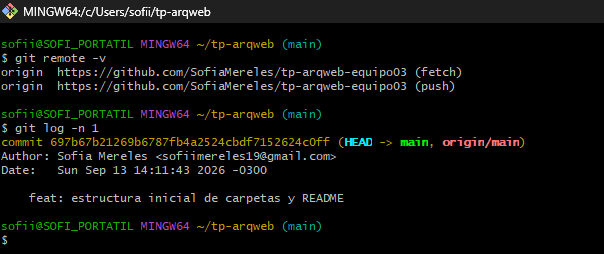
\includegraphics[width=0.85\textwidth]{F1-E1_github_repo.png}
    \caption{F1-E1: Comandos ejecutados en la terminal para la vinculación del repositorio local.}
    \label{fig:F1-E1}
\end{figure}

\begin{figure}[H]
    \centering
    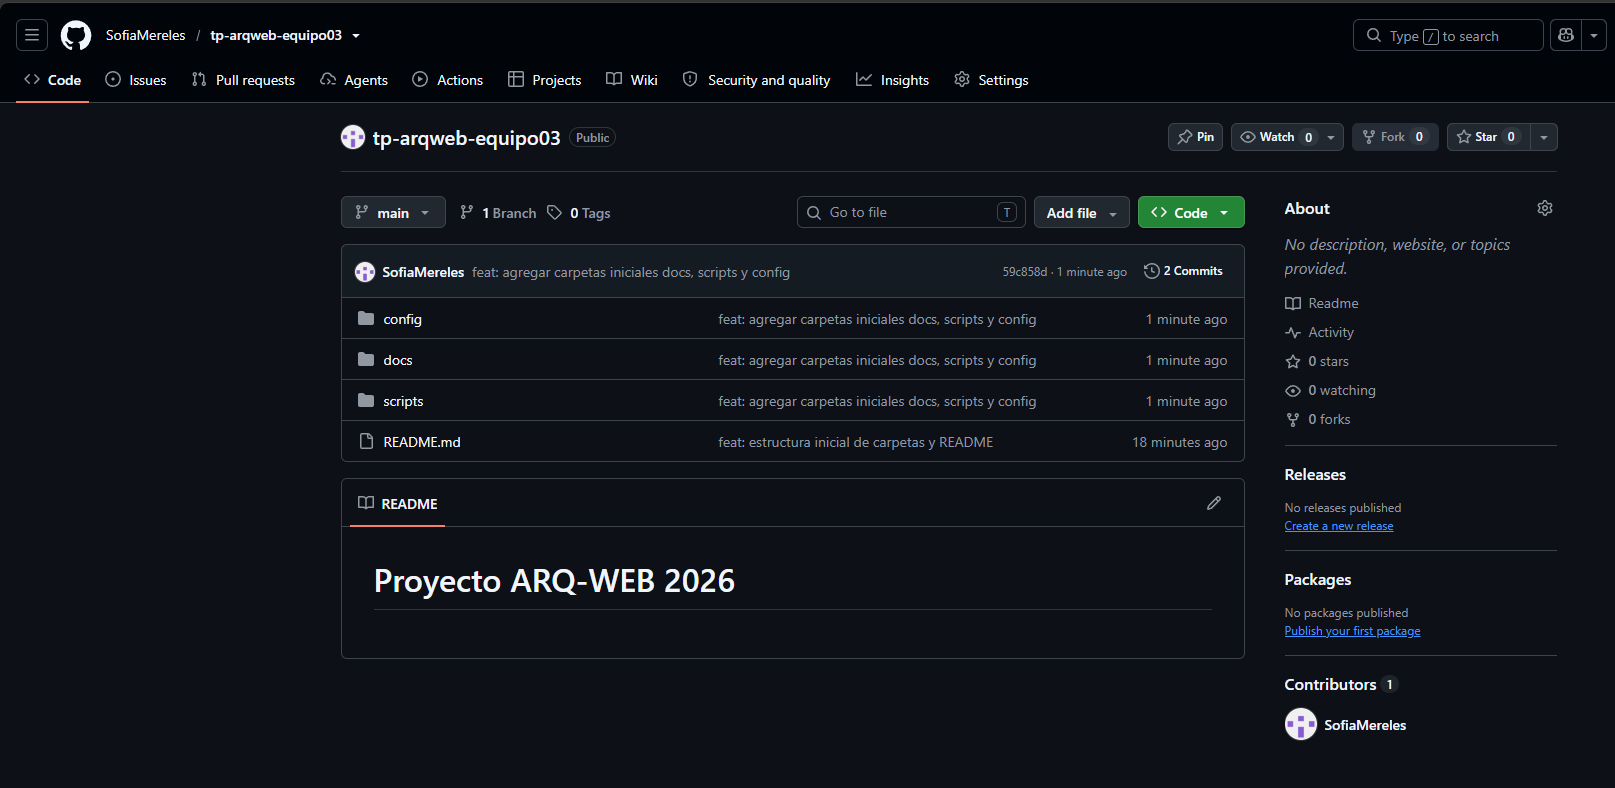
\includegraphics[width=0.85\textwidth]{F1-E2_github_repo.png}
    \caption{F1-E2: Vista web del repositorio público en GitHub con la estructura de directorios.}
    \label{fig:F1-E2}
\end{figure}

\subsection{Especificaciones de la Máquina Virtual}
\begin{itemize}[leftmargin=1.5em]
    \item \textbf{Sistema Operativo:} Ubuntu Server 26.04 LTS (Kernel Linux 6.8.0 / 7.0.0-generic)
    \item \textbf{Recursos de Hardware:} 2 vCPU, 4096 MB RAM, 20 GB Disco SSD.
    \item \textbf{Adaptador de Red:} Virtual Network Adapter en Modo Puente (\textit{Bridged}).
\end{itemize}

\begin{figure}[H]
    \centering
    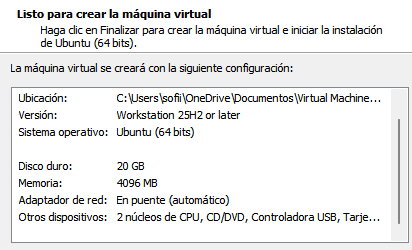
\includegraphics[width=0.82\textwidth]{F1-E3_vmware_hardware.png}
    \caption{F1-E3: Configuración de hardware y red en VMware Workstation.}
    \label{fig:F1-E3}
\end{figure}

\begin{figure}[H]
    \centering
    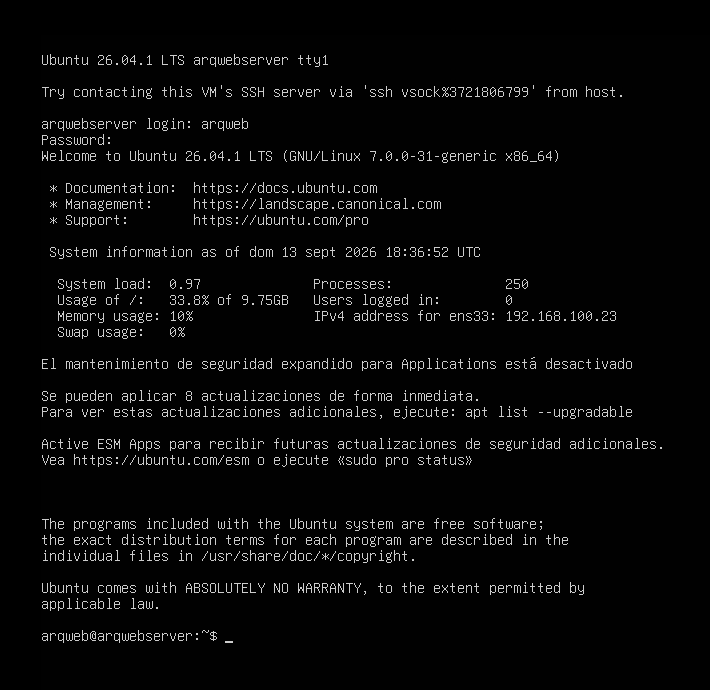
\includegraphics[width=0.82\textwidth]{F1-E4_ubuntu_login.png}
    \caption{F1-E4: Consola de Ubuntu Server operativa con el usuario no-root iniciado.}
    \label{fig:F1-E4}
\end{figure}

\subsection{Línea Base de Red y Direccionamiento}
Mediante el adaptador en modo puente, la máquina virtual obtuvo la dirección IP \texttt{192.168.100.23/24} asignada por el servidor DHCP de la red LAN local.

\begin{figure}[H]
    \centering
    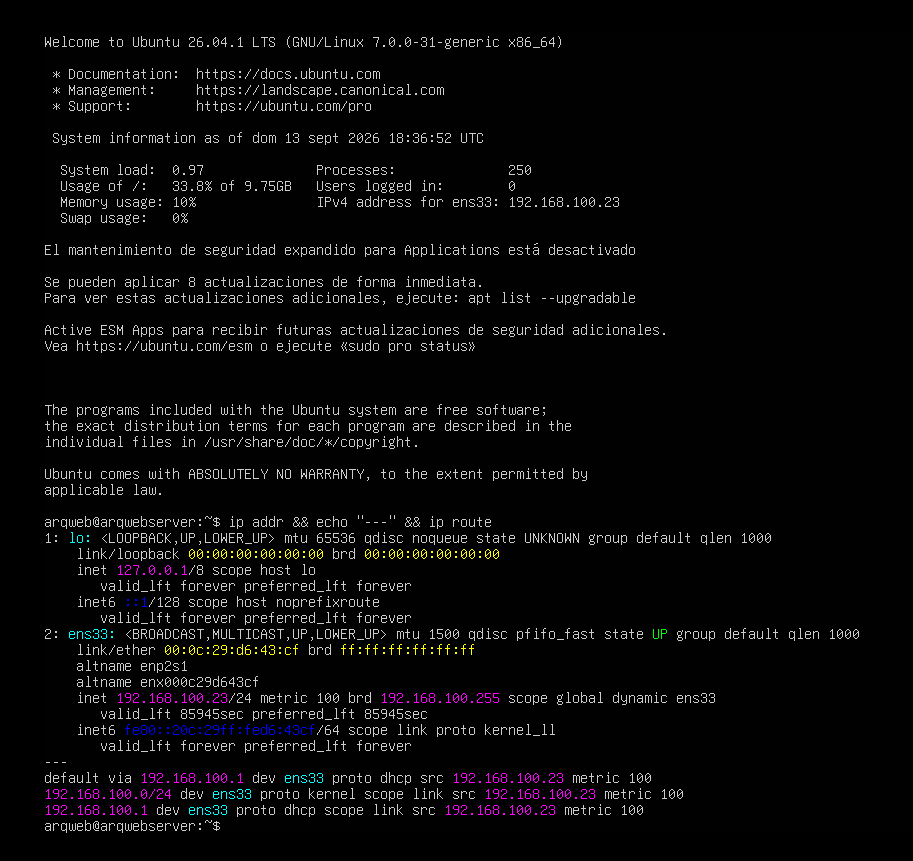
\includegraphics[width=0.85\textwidth]{F1_E5_ip_addr_route.png}
    \caption{F1-E5: Salida del comando \texttt{ip addr} e \texttt{ip route} en Ubuntu Server.}
    \label{fig:F1-E5}
\end{figure}

\begin{figure}[H]
    \centering
    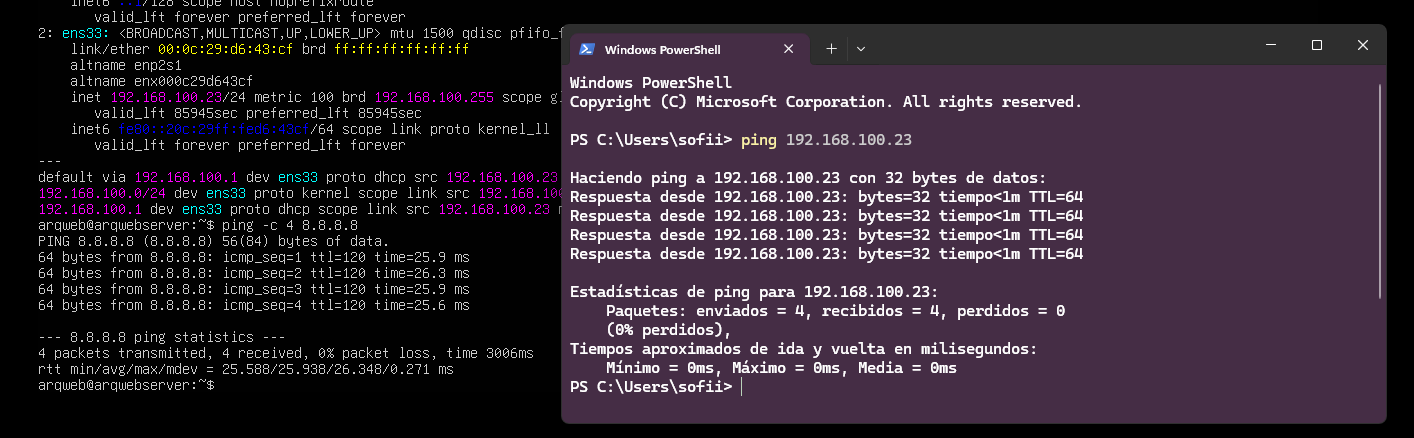
\includegraphics[width=0.85\textwidth]{F1-E6_ping_conectividad.png}
    \caption{F1-E6: Pruebas de conectividad ICMP bidireccional y salida a Internet.}
    \label{fig:F1-E6}
\end{figure}

\begin{figure}[H]
    \centering
    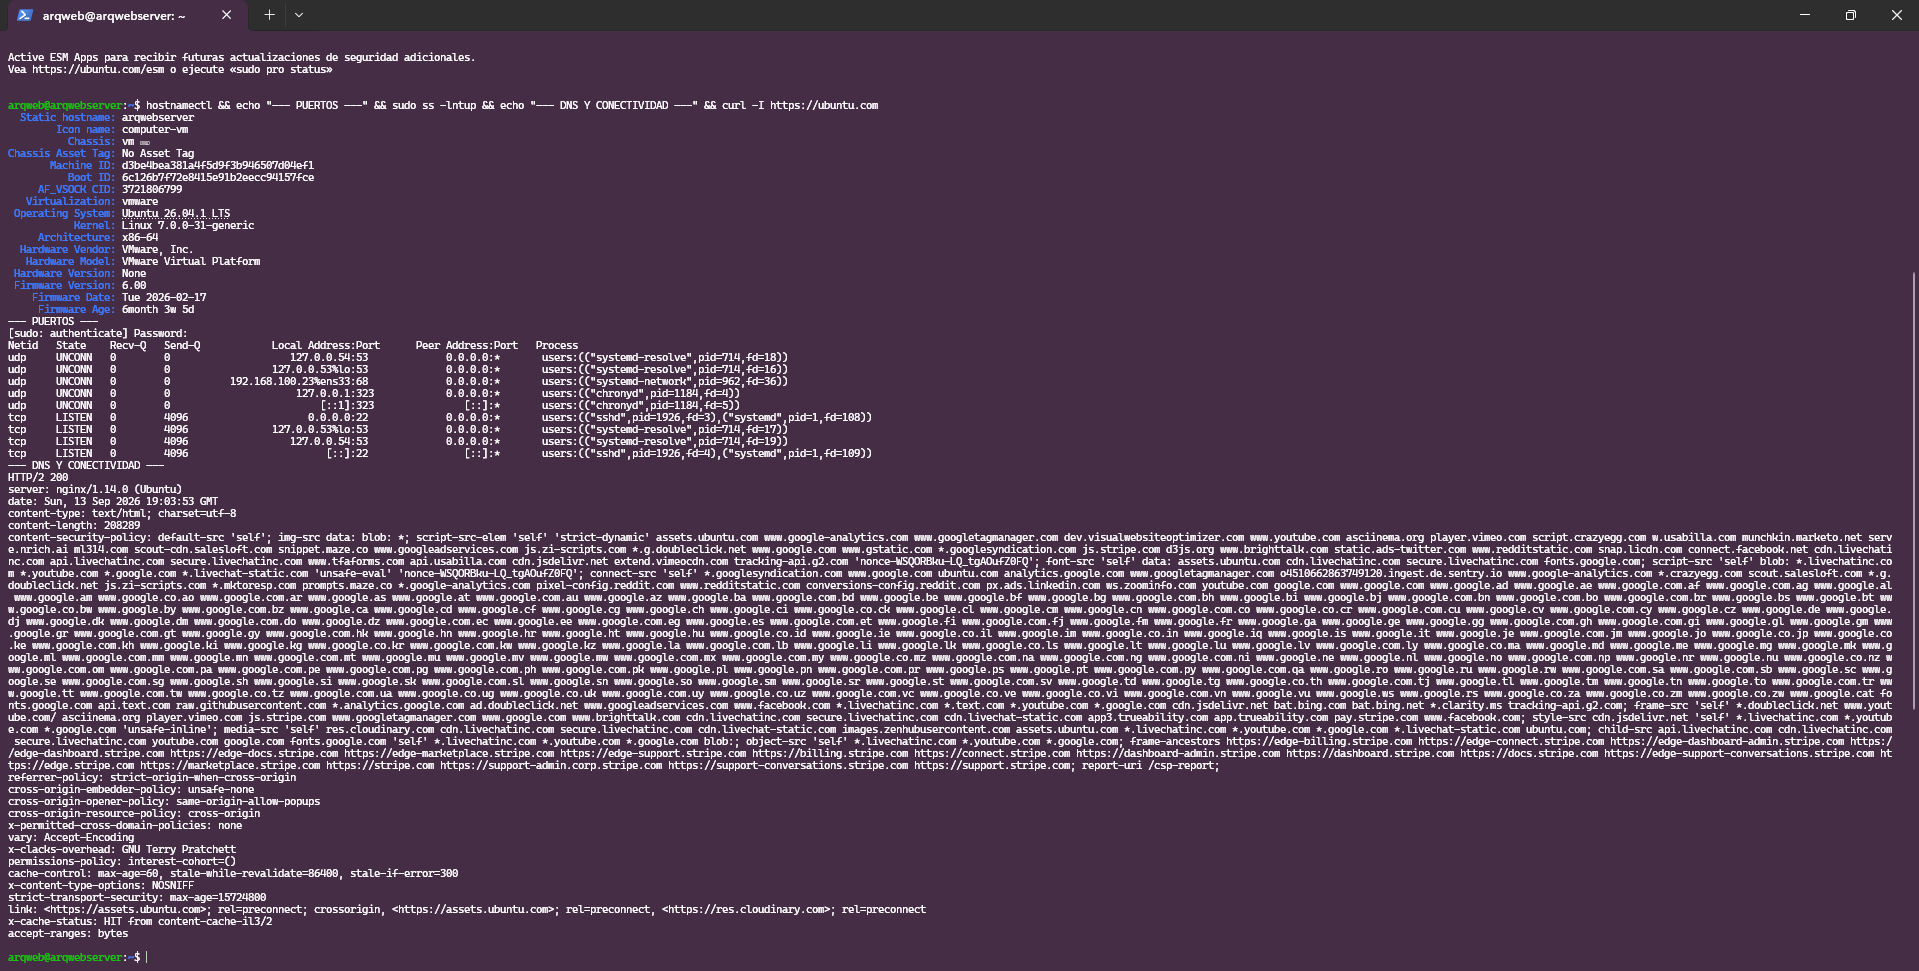
\includegraphics[width=0.85\textwidth]{F1-E7_puertos_dns.png}
    \caption{F1-E7: Verificación del estado del sistema, puerto 22 SSH y resolución DNS.}
    \label{fig:F1-E7}
\end{figure}

\newpage
% =======================================================================
% SECCIÓN 5: DESPLIEGUE Y CONFIGURACIÓN DE SERVICIOS (FASE 2)
% =======================================================================
\section{Despliegue y Configuración de Servicios (Fase 2)}

En esta fase se llevó a cabo el despliegue del stack LNMP (Linux, Nginx, MariaDB, PHP 8.5-FPM) y la instalación completa de BookStack. A continuación se detalla técnicamente el procedimiento ejecutado en cada etapa.

\subsection{Estado Inicial de los Servicios (F2-E1)}
Antes de iniciar la instalación de los componentes web, se realizó una auditoría del estado inicial de los puertos y servicios en escucha mediante el comando \texttt{ss -tulpn > puerto\_antes.txt}. Como se observa en la Figura \ref{fig:F2-E1}, únicamente se encontraban activos el servicio OpenSSH en el puerto TCP 22 y el resolvedor de nombres local en el puerto UDP 53. Al intentar realizar una conexión HTTP local mediante \texttt{curl -I http://192.168.100.23}, el sistema retornó un rechazo explícito de conexión (\textit{Connection refused}), confirmando que no existía ningún servidor web activo previo al despliegue.

\begin{figure}[H]
    \centering
    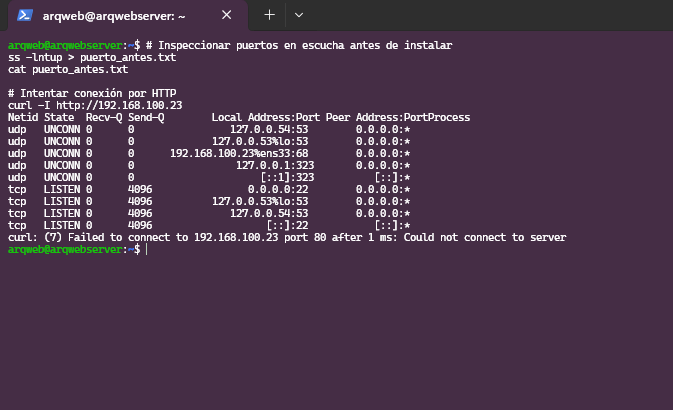
\includegraphics[width=0.90\textwidth]{F2-E1_antes_servicios.png}
    \caption{F2-E1: Verificación del estado inicial de los puertos antes de la instalación del stack.}
    \label{fig:F2-E1}
\end{figure}

\subsection{Verificación de Versiones de Runtime (F2-E2)}
Se procedió a la instalación de los paquetes del stack LNMP utilizando el gestor \texttt{apt}. Posterior a la instalación, se ejecutó una verificación unificada de las versiones del servidor web, del intérprete PHP y del motor de base de datos. Como evidencia la Figura \ref{fig:F2-E2}, el entorno quedó configurado con \textbf{Nginx 1.28.3}, \textbf{PHP 8.5.4-cli} (con Zend OPcache v8.5.4 activo) y \textbf{MariaDB 11.8.6}. Todos los demonios correspondientes fueron habilitados en el gestor de servicios \texttt{systemd} para garantizar su inicio automático.

\begin{figure}[H]
    \centering
    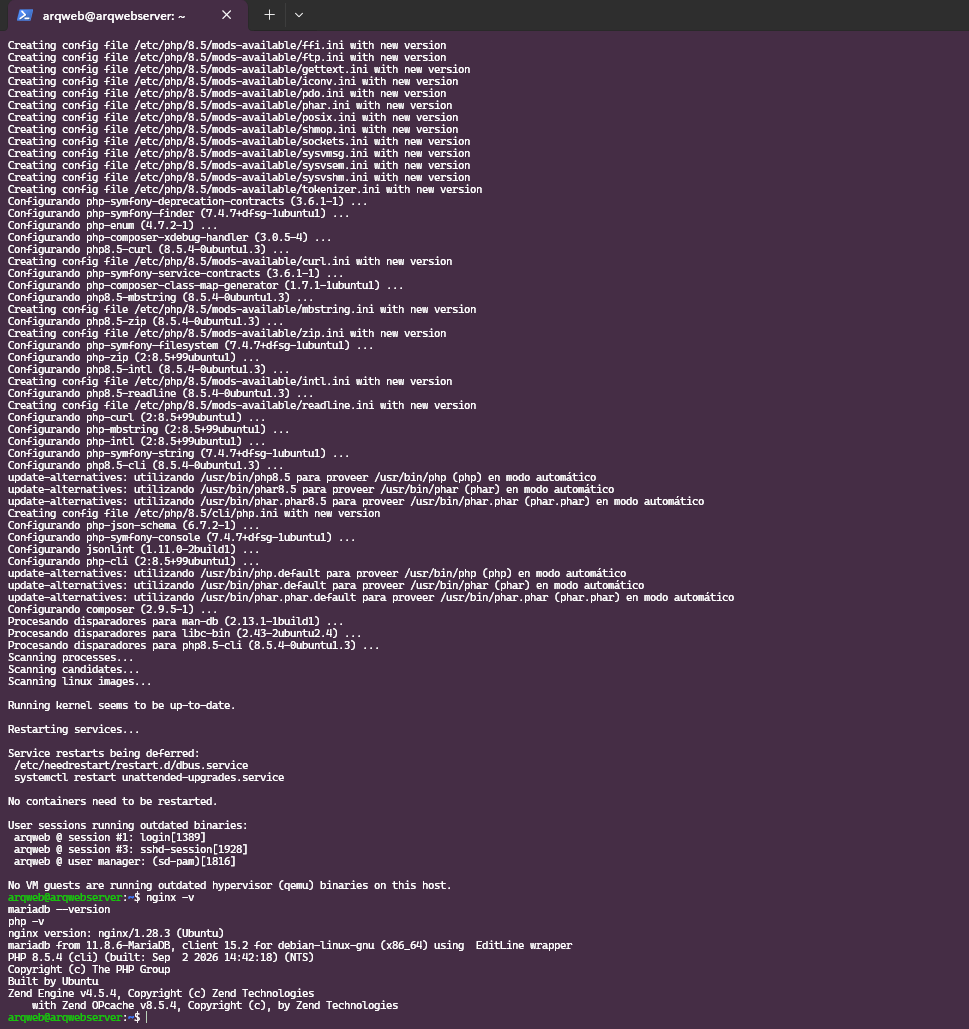
\includegraphics[width=0.75\textwidth]{F2-E2_versiones_runtime.png}
    \caption{F2-E2: Comprobación de versiones activas de Nginx, PHP 8.5 y MariaDB.}
    \label{fig:F2-E2}
\end{figure}

\subsection{Creación y Configuración de la Base de Datos (F2-E3)}
Para dar soporte a la capa de persistencia de BookStack, se ingresó al gestor de base de datos MariaDB mediante la consola administrativa (\texttt{sudo mysql}). Se creó la base de datos relacional \texttt{bookstack\_db} y se generó el usuario dedicado \texttt{bookstack\_user} autenticado localmente (\texttt{@localhost}). Se otorgaron todos los privilegios sobre dicha base de datos y se aplicó la instrucción \texttt{FLUSH PRIVILEGES;}. La ejecución de \texttt{SHOW DATABASES;} confirmó la correcta creación de la estructura, tal como se aprecia en la Figura \ref{fig:F2-E3}.

\begin{figure}[H]
    \centering
    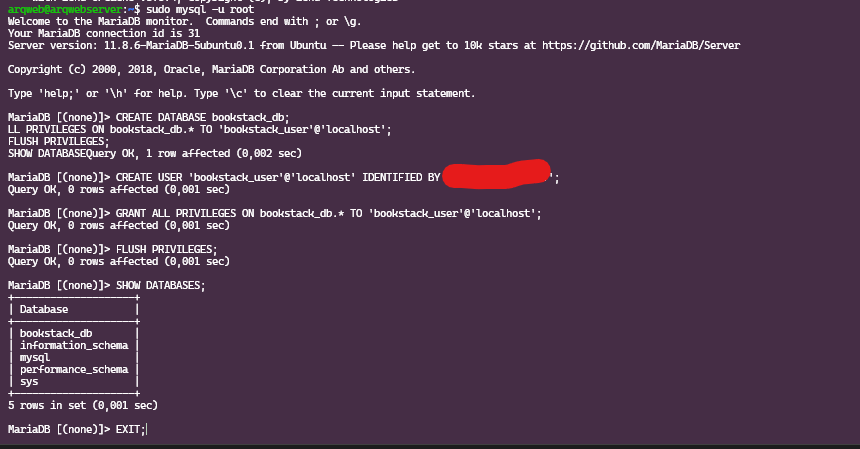
\includegraphics[width=0.88\textwidth]{F2-E3_mariadb_database.png}
    \caption{F2-E3: Sentencias SQL para la creación del esquema y asignación de permisos.}
    \label{fig:F2-E3}
\end{figure}

\subsection{Ejecución de Migraciones de BookStack / Laravel (F2-E4)}
Se desplegó el código fuente de BookStack Release v26.05.4 en la ruta \texttt{/var/www/bookstack}, asignando la propiedad de los archivos al usuario del servidor web (\texttt{www-data:www-data}) y otorgando permisos de escritura (\texttt{775}) sobre los directorios \texttt{storage} y \texttt{bootstrap/cache}. Se creó el archivo de entorno \texttt{.env} vinculando las credenciales de MariaDB y se generó la clave criptográfica de la aplicación mediante \texttt{php artisan key:generate --force}. Posteriormente, se ejecutó la migración del esquema utilizando \texttt{php artisan migrate --force}. Como demuestra la Figura \ref{fig:F2-E4}, la herramienta Artisan ejecutó exitosamente más de 80 migraciones de tablas relacionales (\texttt{users}, \texttt{books}, \texttt{pages}, \texttt{roles}, \texttt{activities}, entre otras).

\begin{figure}[H]
    \centering
    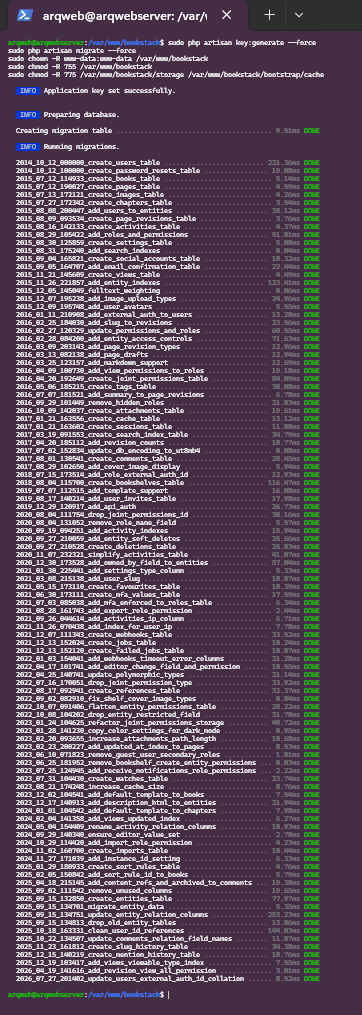
\includegraphics[width=0.55\textwidth]{F2-E4_migracion_laravel.png}
    \caption{F2-E4: Ejecución exitosa de las migraciones de tablas en Laravel para BookStack.}
    \label{fig:F2-E4}
\end{figure}

\subsection{Configuración del Virtual Host y Sintaxis de Nginx (F2-E5)}
Se estructuró el archivo de Virtual Host en \texttt{/etc/nginx/sites-available/bookstack}, configurando la raíz web en \texttt{/var/www/bookstack/public} y derivando la ejecución de archivos PHP al socket Unix de FastCGI (\texttt{/var/run/php/php8.5-fpm.sock}). Se habilitó el sitio creando el enlace simbólico en \texttt{sites-enabled/} y se removió el sitio por defecto. Finalmente, se ejecutó \texttt{sudo nginx -t} para validar la sintaxis de la configuración. La Figura \ref{fig:F2-E5} certifica que el test resultó exitoso (\textit{syntax is ok / test is successful}).

\begin{figure}[H]
    \centering
    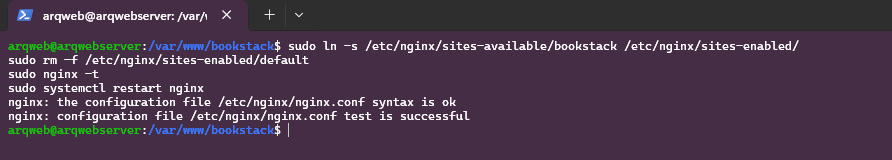
\includegraphics[width=0.90\textwidth]{F2-E5_nginx_sintaxis.png}
    \caption{F2-E5: Verificación de sintaxis exitosa del archivo de configuración de Nginx.}
    \label{fig:F2-E5}
\end{figure}

\subsection{Estado Final de Servicios y Puertos en Escucha (F2-E6)}
Tras reiniciar el servidor web (\texttt{systemctl restart nginx}), se ejecutó una inspección detallada de sockets activos con \texttt{ss -tulpn}. Como ilustra la Figura \ref{fig:F2-E6}, se constató que el proceso \texttt{nginx} se encuentra escuchando en el puerto TCP 80 (\texttt{0.0.0.0:80}) y el motor \texttt{mariadbd} se mantiene activo únicamente en la interfaz de bucle invertido TCP 3306 (\texttt{127.0.0.1:3306}), garantizando el aislamiento de la base de datos de la red pública.

\begin{figure}[H]
    \centering
    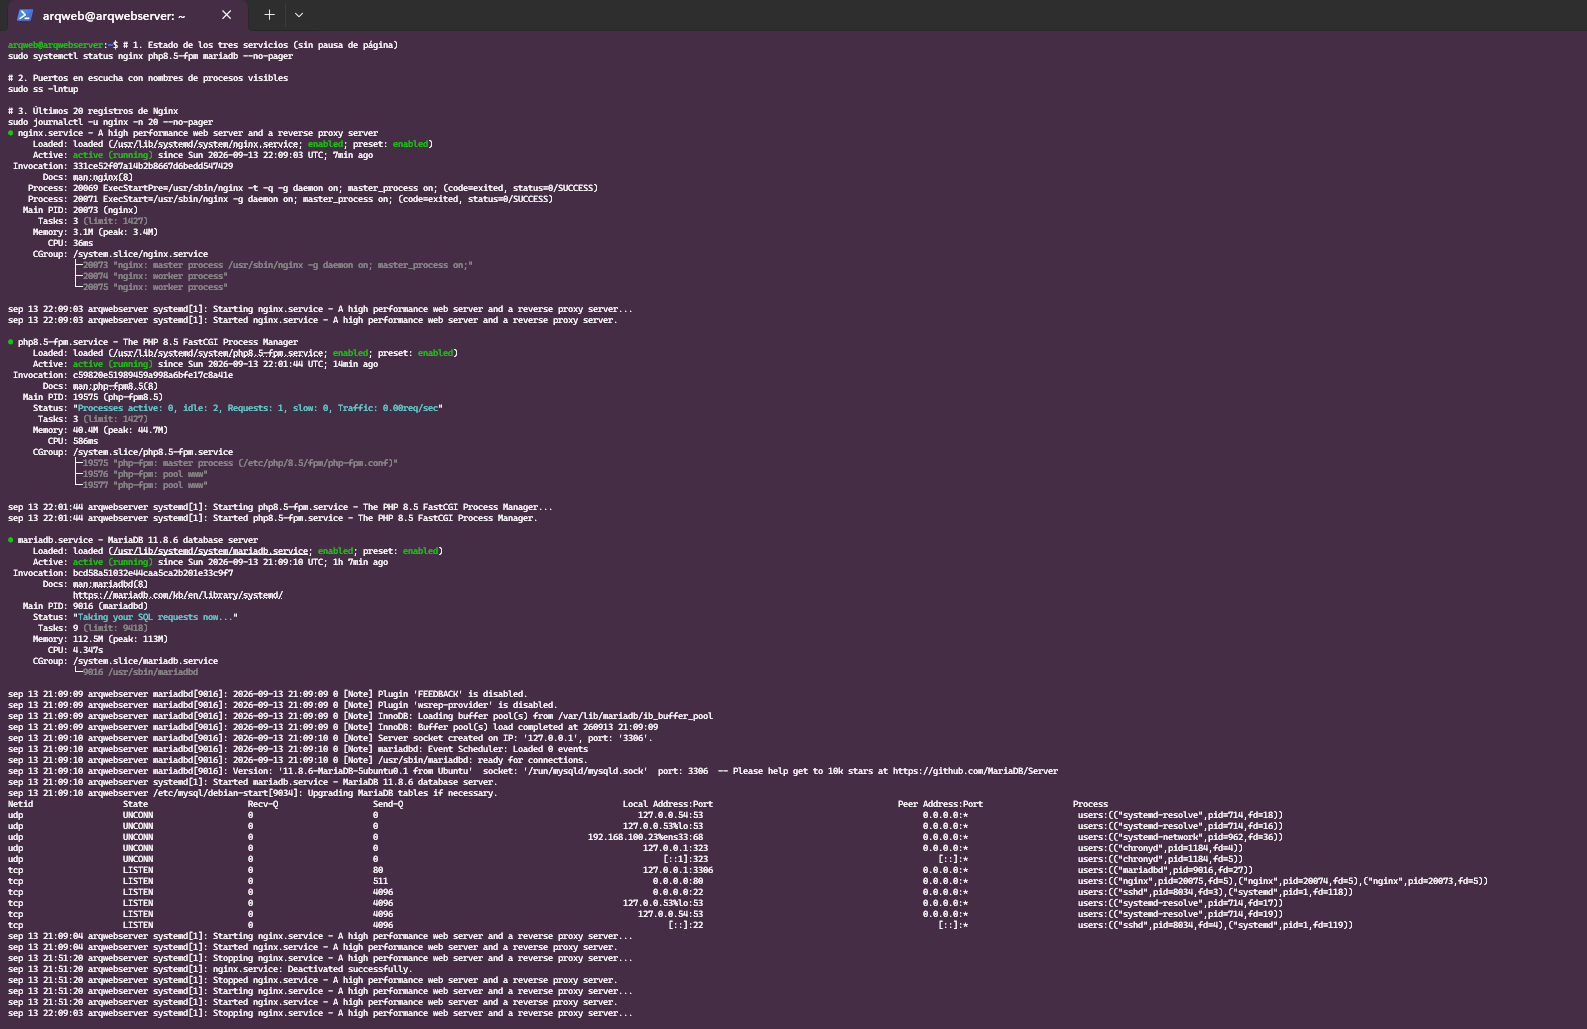
\includegraphics[width=0.95\textwidth]{F2-E6_despues_servicios_puertos.png}
    \caption{F2-E6: Inspección final de servicios activos y sockets en los puertos TCP 80 y TCP 3306.}
    \label{fig:F2-E6}
\end{figure}

\subsection{Pruebas de Conectividad HTTP y Verificación Web Final (F2-E7)}
Para finalizar la Fase 2, se realizó la prueba de conectividad HTTP a nivel de consola y navegador. En primer lugar, la ejecución de \texttt{curl -I http://192.168.100.23} retornó un código de respuesta \texttt{HTTP/1.1 200 OK} con las cabeceras emitidas por Nginx y la inicialización de la cookie de sesión de Laravel (Figura \ref{fig:F2-E7_curl}). En segundo lugar, se accedió a la URL desde la máquina anfitriona; la Figura \ref{fig:F2-E7_final} demuestra la renderización completa del formulario de inicio de sesión de BookStack y el panel DevTools de red registrando el estado 200 OK en la descarga de todos los recursos estáticos.

\begin{figure}[H]
    \centering
    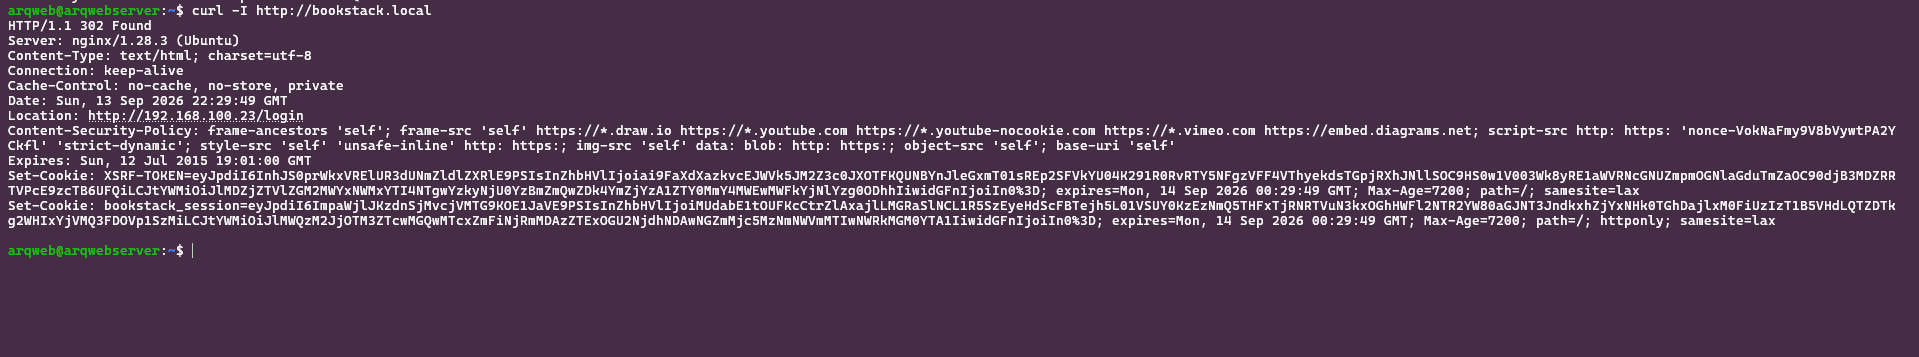
\includegraphics[width=0.85\textwidth]{F2-E7_curl_headers.png}
    \caption{F2-E7a: Respuesta del servidor web mostrando encabezados HTTP mediante \texttt{curl}.}
    \label{fig:F2-E7_curl}
\end{figure}

\begin{figure}[H]
    \centering
    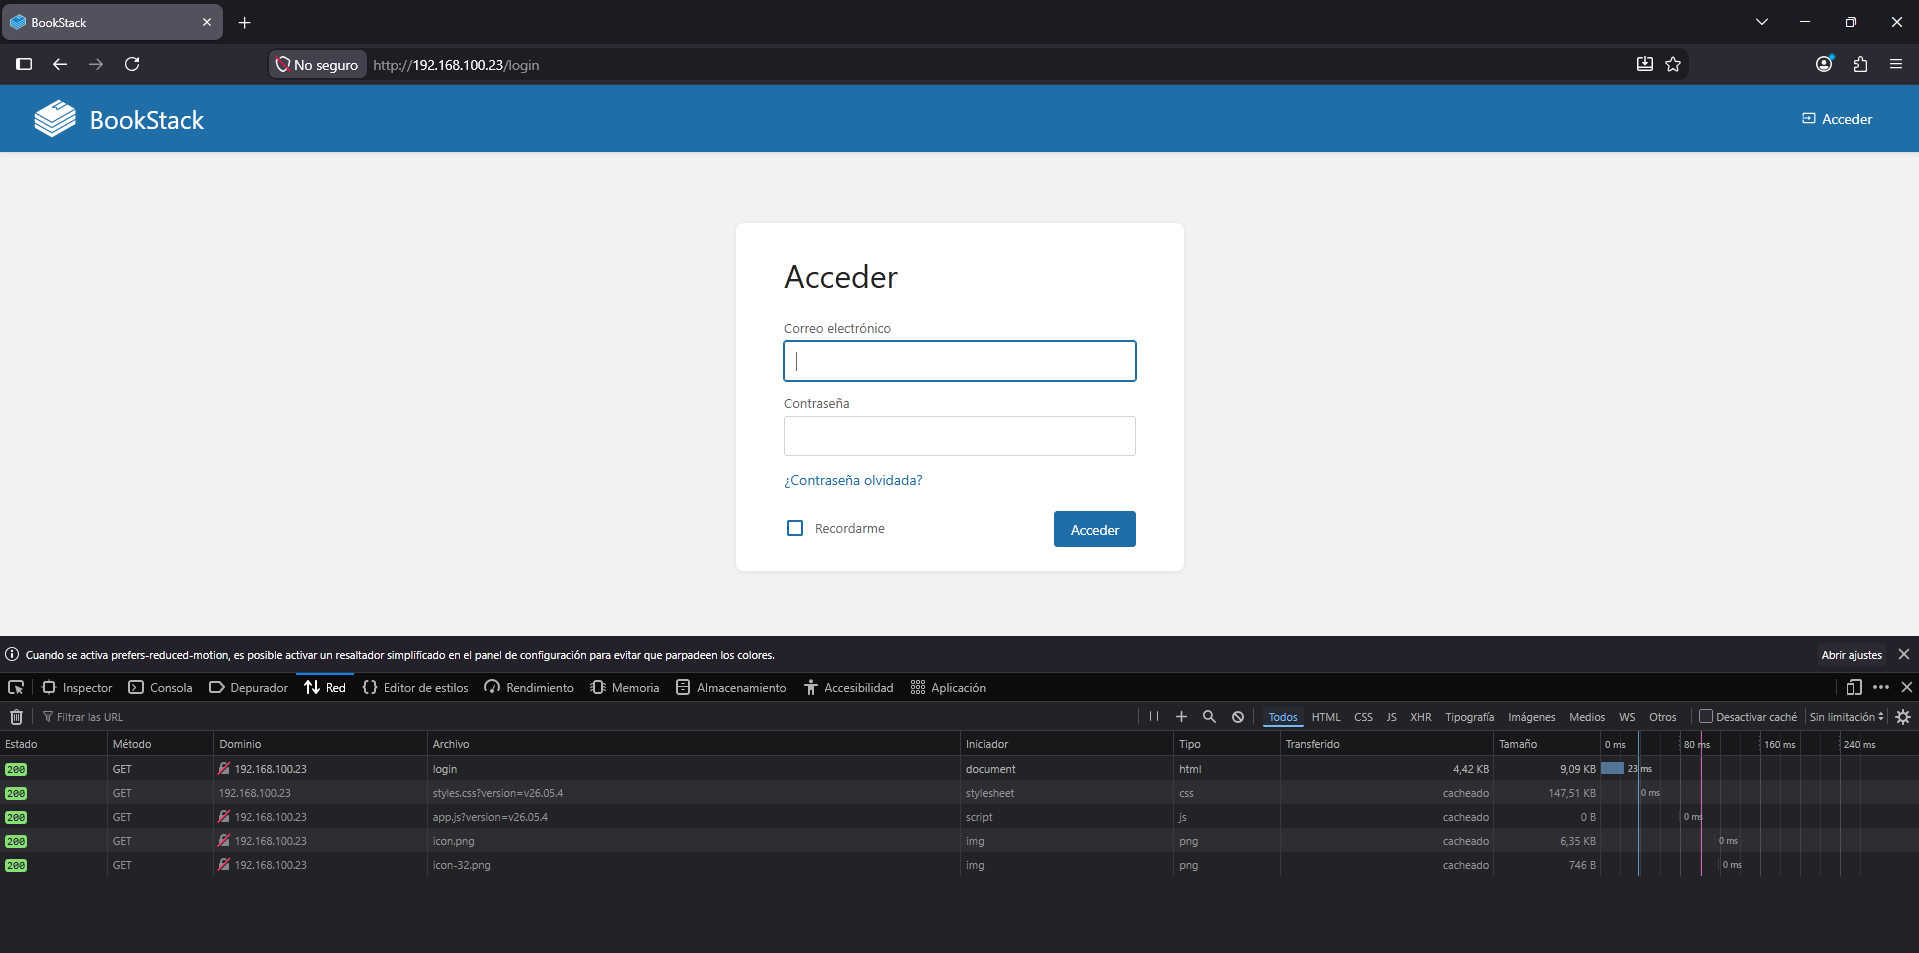
\includegraphics[width=0.95\textwidth]{F2-E7_verificacion_final.png}
    \caption{F2-E7b: Carga completa de la interfaz de login de BookStack y panel DevTools.}
    \label{fig:F2-E7_final}
\end{figure}

\newpage
% =======================================================================
% SECCIÓN 6: SEGURIDAD, RENDIMIENTO Y ANÁLISIS DE RED (FASE 3)
% =======================================================================
\section{Seguridad, Rendimiento y Análisis de Red (Fase 3)}

En esta sección se detalla la implementación del protocolo HTTPS sobre TLS 1.3, la resolución de nombres local, la optimización de cabeceras/caché, las mediciones de latencia y el análisis de la traza de red capturada.

\subsection{Resolución de Nombres Local y Certificado X.509}
Para simular un entorno de producción con un Fully Qualified Domain Name (FQDN), se asignó el dominio \texttt{bookstack.local} asociándolo a la dirección IP \texttt{192.168.100.23} dentro del archivo de mapeo estático del sistema (\texttt{/etc/hosts}).

\begin{figure}[H]
    \centering
    \includegraphics[width=0.85\textwidth]{"F2-E1-Resolucion de nombre.png"}
    \caption{F3-E1: Configuración de resolución de nombres en \texttt{/etc/hosts} y prueba con \texttt{ping bookstack.local}.}
    \label{fig:F3-E1}
\end{figure}

En la Figura \ref{fig:F3-E1} (Evidencia F3-E1), se comprueba que el nombre de dominio resuelve correctamente hacia la IP de la máquina virtual con un tiempo de latencia nulo. A continuación, se generó un certificado digital X.509 autofirmado mediante OpenSSL, especificando la extensión \textit{Subject Alternative Name} (SAN):

\begin{figure}[H]
    \centering
    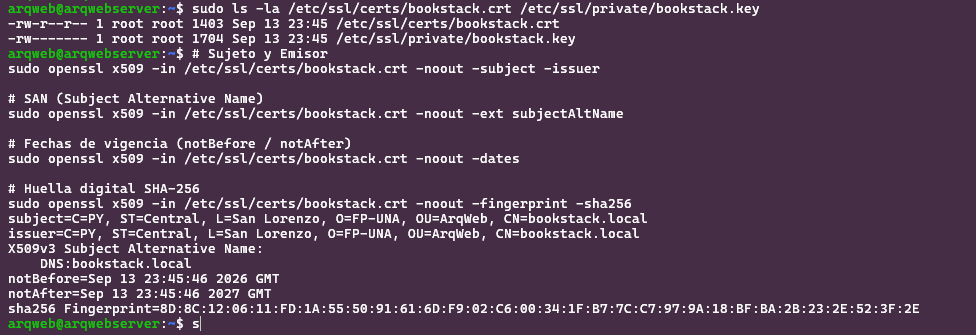
\includegraphics[width=0.92\textwidth]{F2-E2-Certificado-local.png}
    \caption{F3-E2: Inspección del certificado X.509 emitido con OpenSSL (\texttt{CN=bookstack.local}, RSA 2048 bits).}
    \label{fig:F3-E2}
\end{figure}

Como evidencia la Figura \ref{fig:F3-E2} (Evidencia F3-E2), la inspección del archivo \texttt{/etc/ssl/certs/bookstack.crt} confirma la validez del certificado, vigencia de un año, algoritmo \texttt{sha256WithRSAEncryption} y huella digital correspondiente.

\paragraph{Análisis de la Cadena de Confianza y Advertencias del Navegador:}
Al acceder a un sitio configurado con un certificado autofirmado, el navegador emite una advertencia de seguridad (\textit{"La conexión no es privada"}). Esto ocurre porque la Autoridad Certificadora (CA) emisora es la misma entidad que el sujeto (\texttt{Issuer = Subject}), por lo que la CA no se encuentra dentro del almacén de confianza del sistema operativo cliente (\textit{Root CA Store}). En producción, este paso se sustituye por la emisión de un certificado validado por una CA pública (ej. Let's Encrypt).

\subsection{Configuración de la Aplicación y Server Block en Nginx}
Para garantizar la coherencia de la aplicación Laravel con la capa de transporte segura, se actualizó el archivo de entorno global \texttt{.env} de BookStack ajustando la variable de URL base:

\begin{figure}[H]
    \centering
    \includegraphics[width=0.85\textwidth]{"F3-E3-VERIFICACION APP_URL.png"}
    \caption{F3-E3: Verificación de la variable de entorno \texttt{APP\_URL=https://bookstack.local} en el archivo \texttt{.env}.}
    \label{fig:F3-E3}
\end{figure}

En la Figura \ref{fig:F3-E3} (Evidencia F3-E3), el comando \texttt{grep} confirma que los recursos estáticos, enlaces absolutos y cookies de sesión sean generados bajo el esquema seguro HTTPS. Posteriormente, se reestructuró el archivo de bloque de servidor de Nginx dividiéndolo en dos bloques \texttt{server}:
\begin{enumerate}[leftmargin=1.5em]
    \item \textbf{Bloque HTTP (Puerto 80):} Captura todas las peticiones inseguras e inyecta una redirección permanente \texttt{HTTP 301 Moved Permanently} hacia \texttt{https://bookstack.local\$request\_uri}.
    \item \textbf{Bloque HTTPS (Puerto 443):} Configura la escucha en modo SSL (\texttt{listen 443 ssl;}), enlaza la clave privada y certificado, limita los protocolos a \textbf{TLS 1.2} y \textbf{TLS 1.3}, y deriva la ejecución PHP al socket Unix de PHP-FPM.
\end{enumerate}

\begin{figure}[H]
    \centering
    \includegraphics[width=0.75\textwidth]{"F3-E4-Virtual Host de Nginx.png"}
    \caption{F3-E4: Edición del Server Block en Nginx habilitando SSL/TLS 1.3 en el puerto 443 y redirección HTTP 301.}
    \label{fig:F3-E4}
\end{figure}

\subsection{Evaluación Experimental de Rendimiento HTTPS}
Se ejecutó un script en Bash realizando 10 iteraciones consecutivas mediante el comando \texttt{curl -w} para descomponer los tiempos de conexión en cada fase del modelo de red:

\begin{figure}[H]
    \centering
    \includegraphics[width=0.95\textwidth]{"F2-E5-Medición de rendimiento.png"}
    \caption{F3-E5: Ejecución secuencial de 10 mediciones de rendimiento con \texttt{curl} sobre HTTPS.}
    \label{fig:F3-E5}
\end{figure}

Como muestra la Figura \ref{fig:F3-E5} (Evidencia F3-E5), se registraron los métricos consolidados en la Tabla \ref{tab:rendimiento}.

\begin{table}[h!]
\centering
\small
\rowcolors{2}{LightGrayBG}{white}
\begin{tabular}{|c|c|c|c|c|}
\hline
\rowcolor{NavyPrimary} \color{white}\textbf{Iteración} & \color{white}\textbf{DNS Lookup (s)} & \color{white}\textbf{TCP Connect (s)} & \color{white}\textbf{TLS Handshake (s)} & \color{white}\textbf{Tiempo Total (s)} \\ \hline
1 & 0.000662 & 0.002223 & 0.012722 & 0.038471 \\ \hline
2 & 0.000432 & 0.000560 & 0.012620 & 0.028179 \\ \hline
3 & 0.000469 & 0.002177 & 0.007113 & 0.022014 \\ \hline
4 & 0.000450 & 0.000638 & 0.005013 & 0.019766 \\ \hline
5 & 0.000364 & 0.000483 & 0.005072 & 0.021375 \\ \hline
6 & 0.000421 & 0.000543 & 0.005405 & 0.021081 \\ \hline
7 & 0.000473 & 0.001106 & 0.005936 & 0.021663 \\ \hline
8 & 0.000706 & 0.000891 & 0.005562 & 0.021675 \\ \hline
9 & 0.000405 & 0.000504 & 0.004726 & 0.021620 \\ \hline
10 & 0.000621 & 0.000959 & 0.005881 & 0.021218 \\ \hline
\textbf{Promedio} & \textbf{0.000500s (0.50 ms)} & \textbf{0.001008s (1.01 ms)} & \textbf{0.007005s (7.00 ms)} & \textbf{0.023706s (23.71 ms)} \\ \hline
\end{tabular}
\caption{Desglose de tiempos de respuesta en la negociación HTTPS (10 iteraciones).}
\label{tab:rendimiento}
\end{table}

\paragraph{Interpretación Técnica de los Resultados:}
\begin{itemize}[leftmargin=1.5em]
    \item \textbf{Efecto Calentamiento (\textit{Warm-up}):} La primera medición registró un tiempo total de $38.4\text{ ms}$ debido a la lectura inicial en disco de los certificados y la inicialización de procesos en el worker de PHP-FPM.
    \item \textbf{Optimización por Reuso de Sesión TLS:} A partir de la iteración 4, el tiempo de negociación TLS disminuyó de $12.7\text{ ms}$ a $\sim 5.0\text{ ms}$. Esto se debe al uso de \textit{TLS Session Tickets} en TLS 1.3, eliminando un viaje de ida y vuelta (\textit{RTT}) en reconexiones.
    \item \textbf{Estabilidad:} El sistema demostró un tiempo de procesamiento promedio de **23.71 ms**, manteniendo una desviación estándar mínima en el entorno virtualizado.
\end{itemize}

\subsection{Inspección de Cabeceras HTTP, Compresión y Caché}
Se analizó la respuesta del servidor mediante \texttt{curl -I} enviando la cabecera \texttt{Accept-Encoding: gzip} para auditar las políticas de caché y compresión de datos:

\begin{figure}[H]
    \centering
    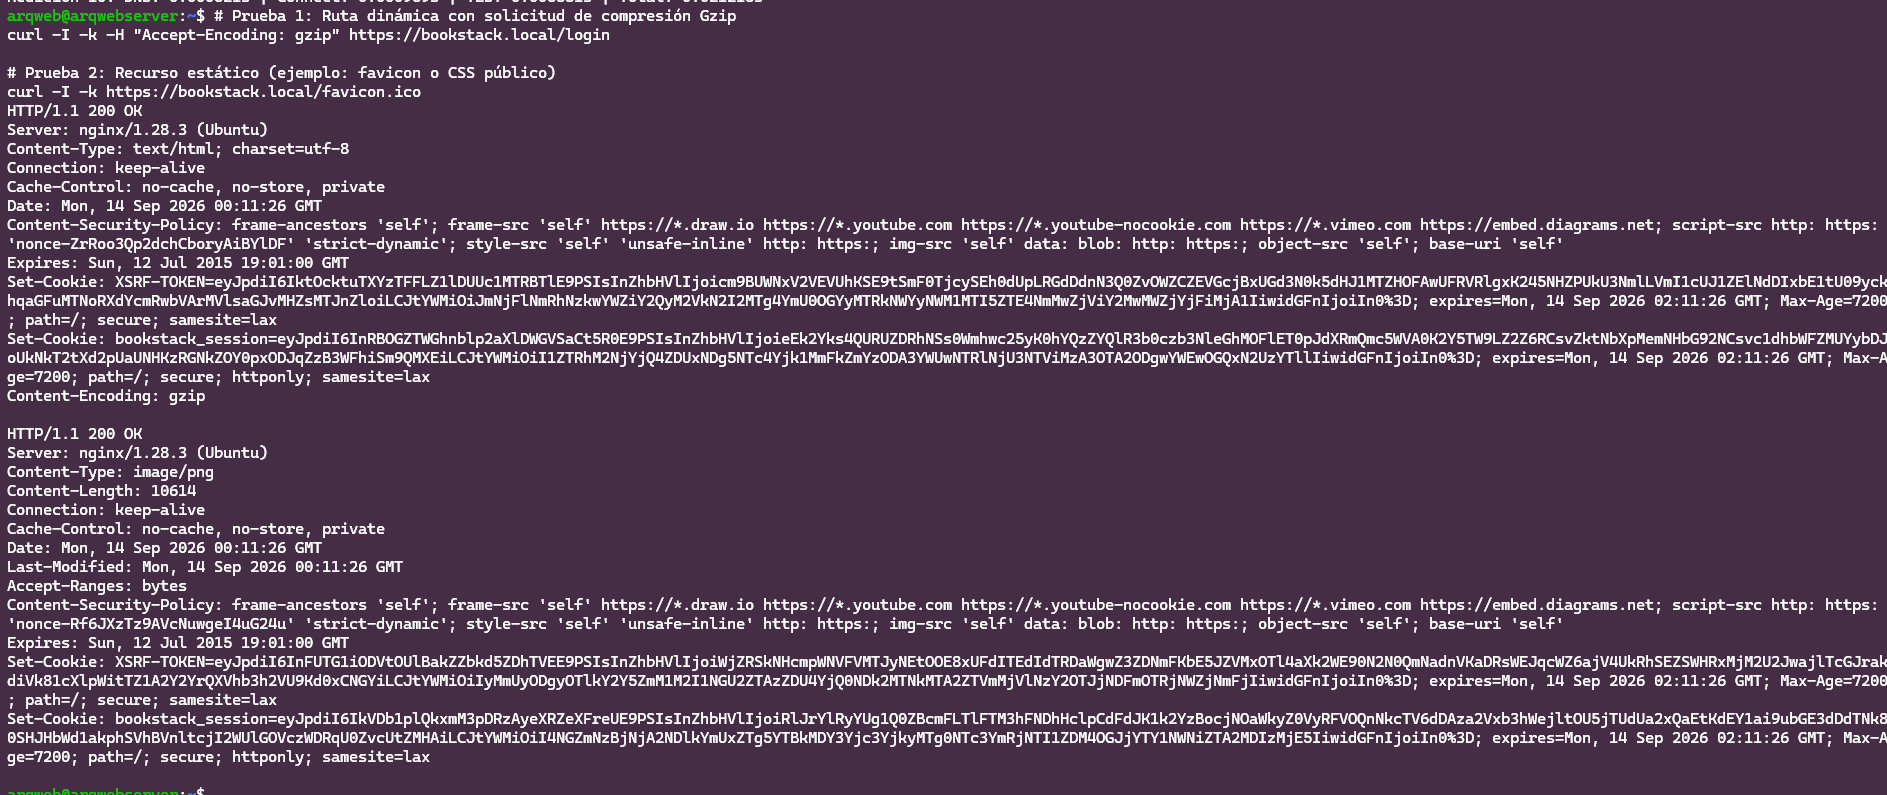
\includegraphics[width=0.95\textwidth]{F3-E6-evidencia_compresion_y_cache.png}
    \caption{F3-E6: Verificación de cabeceras HTTP de respuesta: \texttt{Content-Encoding: gzip}, \texttt{Cache-Control} y cookies.}
    \label{fig:F3-E6}
\end{figure}

Como evidencia la Figura \ref{fig:F3-E6} (Evidencia F3-E6), se identifican los siguientes comportamientos:
\begin{itemize}[leftmargin=1.5em]
    \item \textbf{Compresión Dinámica:} La presencia de \texttt{Content-Encoding: gzip} confirma que Nginx comprime el cuerpo HTML antes de la transmisión, reduciendo el consumo de ancho de banda.
    \item \textbf{Caché en Rutas Dinámicas:} La cabecera \texttt{Cache-Control: no-cache, no-store, private} previene que páginas transaccionales con tokens CSRF o cookies de sesión sean almacenadas en proxies intermedios.
    \item \textbf{Atributos de Cookies Seguras:} Las cookies \texttt{XSRF-TOKEN} y \texttt{bookstack\_session} incluyen las directivas \texttt{secure} y \texttt{httponly}, garantizando que solo viajen sobre HTTPS y no sean accesibles mediante código JavaScript de cliente.
    \item \textbf{Validación Condicional 304 (Not Modified):} Para recursos estáticos, Nginx entrega la cabecera \texttt{Last-Modified}. Ante peticiones subsecuentes del cliente con \texttt{If-Modified-Since}, el servidor responde con \texttt{HTTP 304 Not Modified}, omitiendo el reenvío del archivo.
\end{itemize}

\subsection{Comparativa de Arquitectura: Acceso Directo al Backend vs. Proxy Inverso}

\begin{table}[h!]
\centering
\small
\rowcolors{2}{LightGrayBG}{white}
\begin{tabularx}{\textwidth}{|p{3.2cm}|X|X|}
\hline
\rowcolor{NavyPrimary} \color{white}\textbf{Criterio} & \color{white}\textbf{Acceso Directo (PHP-FPM)} & \color{white}\textbf{Proxy Inverso (Nginx)} \\ \hline
\textbf{Protocolo Soportado} & Exclusivamente protocolo binario \textbf{FastCGI}. No habla HTTP de forma nativa. & \textbf{HTTP/1.1, HTTP/2, HTTPS (TLS 1.2/1.3)}. Traduce HTTP a FastCGI. \\ \hline
\textbf{Terminación TLS} & Sin soporte nativo de cifrado X.509/TLS. Tráfico transmitido en texto plano. & Gestiona el certificado SSL/TLS, descifrado y suites de cifrado simétrico. \\ \hline
\textbf{Archivos Estáticos} & Ineficiente. Carga el intérprete PHP para entregar imágenes, CSS o JS. & Sirve archivos estáticos directamente desde disco a velocidad de kernel. \\ \hline
\textbf{Seguridad / Aislamiento} & Exponer el socket TCP (ej. 9000) abre vectores de Ejecución Remota de Código (RCE). & Aísla el backend, sanitiza encabezados y limita el tamaño de payload. \\ \hline
\end{tabularx}
\caption{Comparativa entre acceso directo al backend PHP-FPM y proxy inverso Nginx.}
\label{tab:comparativa_proxy}
\end{table}

\textbf{Conclusión de Arquitectura:} No es seguro ni técnicamente viable exponer directamente PHP-FPM a la red. Nginx actúa como una capa indispensable de terminación SSL, optimización de caché, entrega de recursos estáticos y protección del motor de la aplicación.

\subsection{Captura y Análisis de Tráfico de Red con \texttt{tcpdump}}
Se registró el tráfico de red mediante la herramienta CLI \texttt{tcpdump} almacenando la transacción en el archivo \texttt{\textasciitilde/transaccion\_tp3.pcap}. Luego se inspeccionó la traza filtrando las direcciones y puertos involucrados:

\begin{figure}[H]
    \centering
    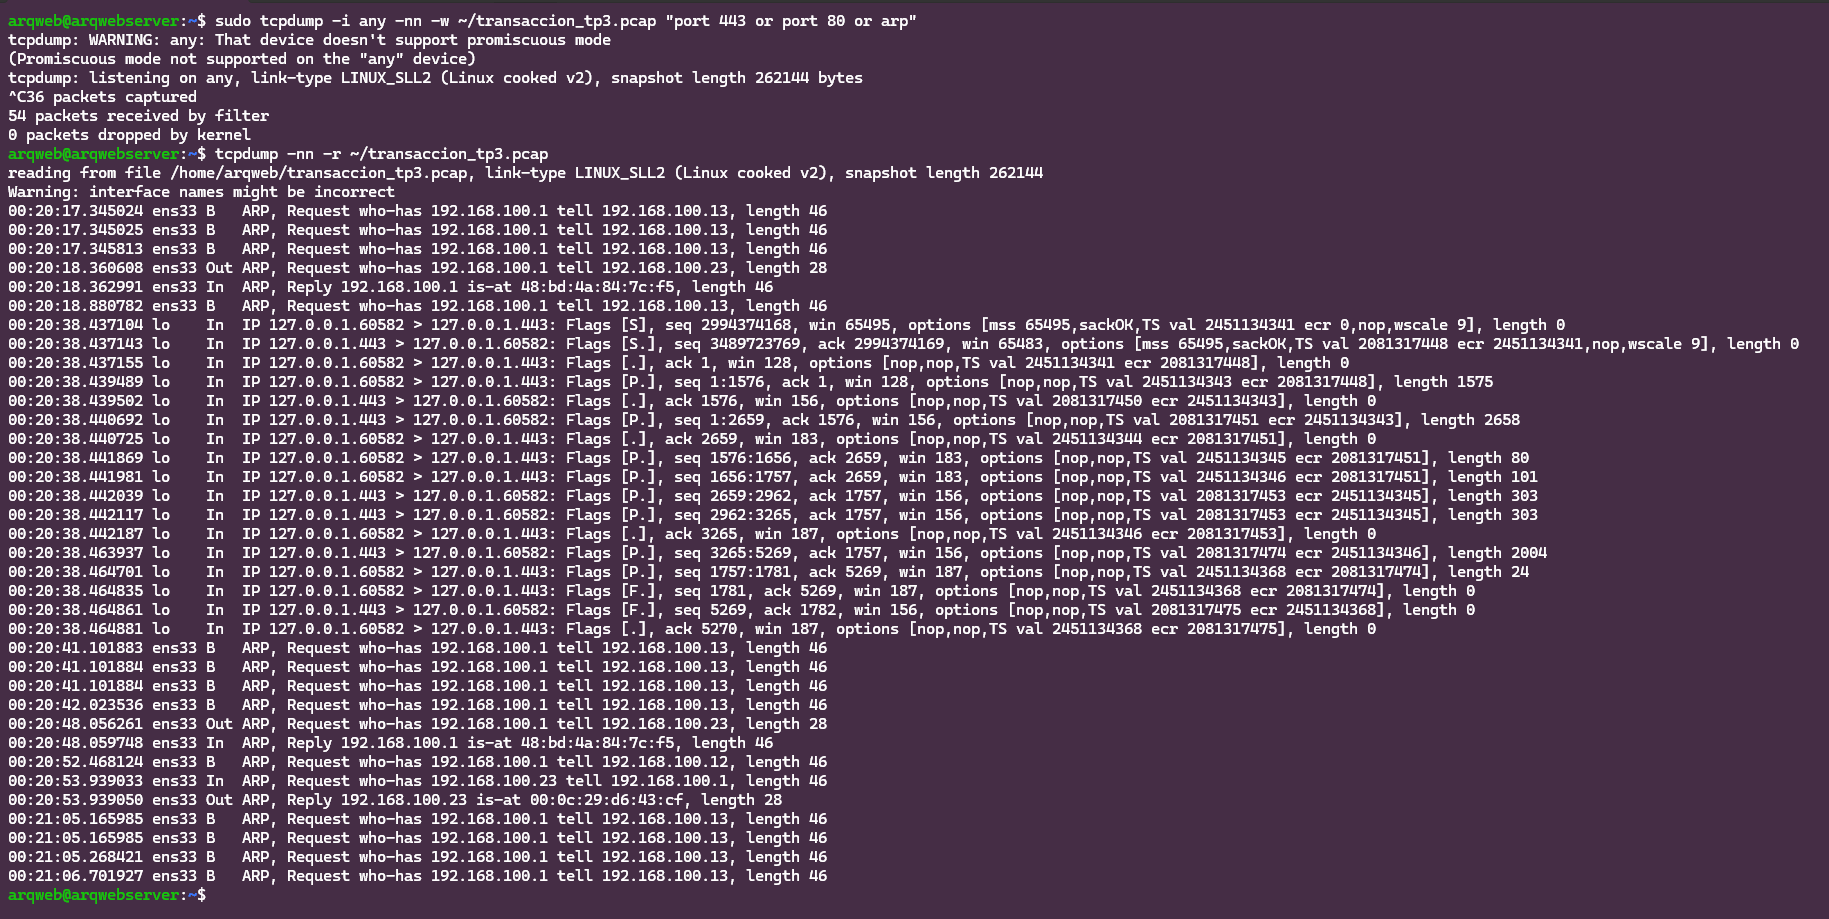
\includegraphics[width=0.98\textwidth]{F2-E7-evidencia_trafico_tcp_tls_arp.png}
    \caption{F3-E7: Traza de paquetes capturada con \texttt{tcpdump} detallando la secuencia ARP, 3-Way Handshake TCP, TLS 1.3 y tramas encriptadas.}
    \label{fig:F3-E7}
\end{figure}

En la Figura \ref{fig:F3-E7} (Evidencia F3-E7) se aprecia el desglose cronológico de las tramas, analizado en detalle en la Tabla \ref{tab:analisis_tcpdump}.

\begin{table}[h!]
\centering
\small
\rowcolors{2}{LightGrayBG}{white}
\begin{tabular}{|c|c|p{3.2cm}|p{5.8cm}|}
\hline
\rowcolor{NavyPrimary} \color{white}\textbf{Marca de Tiempo} & \color{white}\textbf{Capa / Protocolo} & \color{white}\textbf{Banderas / Tipo} & \color{white}\textbf{Descripción Técnica de la Transacción} \\ \hline
\texttt{00:20:18.360} & Capa 2 / ARP & \texttt{Request / Reply} & Consulta \textit{broadcast} para obtener la MAC física del Gateway (\texttt{192.168.100.1}). \\ \hline
\texttt{00:20:38.437} & Capa 4 / TCP & \texttt{Flags [S]} (SYN) & \textbf{Handshake (1/3):} Cliente solicita conexión al puerto HTTPS (\texttt{443}). \\ \hline
\texttt{00:20:38.437} & Capa 4 / TCP & \texttt{Flags [S.]} (SYN-ACK) & \textbf{Handshake (2/3):} Nginx confirma la disponibilidad para la apertura del socket. \\ \hline
\texttt{00:20:38.437} & Capa 4 / TCP & \texttt{Flags [.]} (ACK) & \textbf{Handshake (3/3):} Establecimiento completo del canal de transporte TCP. \\ \hline
\texttt{00:20:38.439} & Capa 6 / TLS 1.3 & \texttt{Flags [P.]}, 1575 B & \textbf{Client Hello:} Envío de algoritmos de cifrado y extensión SNI (\texttt{bookstack.local}). \\ \hline
\texttt{00:20:38.440} & Capa 6 / TLS 1.3 & \texttt{Flags [P.]}, 2658 B & \textbf{Server Hello:} Nginx envía su certificado X.509 y establece el cifrado simétrico. \\ \hline
\texttt{00:20:38.441} & Capa 7 / HTTPS & \texttt{Application Data} & Intercambio de peticiones y respuestas HTTP/1.1 cifradas e ilegibles en texto plano. \\ \hline
\texttt{00:20:38.464} & Capa 4 / TCP & \texttt{Flags [F.]} (FIN-ACK) & Intercambio de banderas FIN para el cierre ordenado de la sesión TCP. \\ \hline
\end{tabular}
\caption{Análisis detallado de la captura de paquetes de red (\texttt{transaccion\_tp3.pcap}).}
\label{tab:analisis_tcpdump}
\end{table}

\paragraph{Consideración sobre el Tráfico DNS en la Traza:}
En la captura no se registran paquetes de consulta DNS en el puerto 53/UDP. Esto justifica formalmente que la resolución del FQDN \texttt{bookstack.local} fue resuelta a nivel de kernel mediante la tabla del archivo local \texttt{/etc/hosts}, omitiendo la salida a servidores DNS externos.

\subsection{Verificación Final desde Navegador con DevTools (F3-E8)}
Como paso de validación final, se accedió a la plataforma desde el navegador web habilitando el panel de inspección DevTools en la pestaña \textbf{Network}:

\begin{figure}[H]
    \centering
    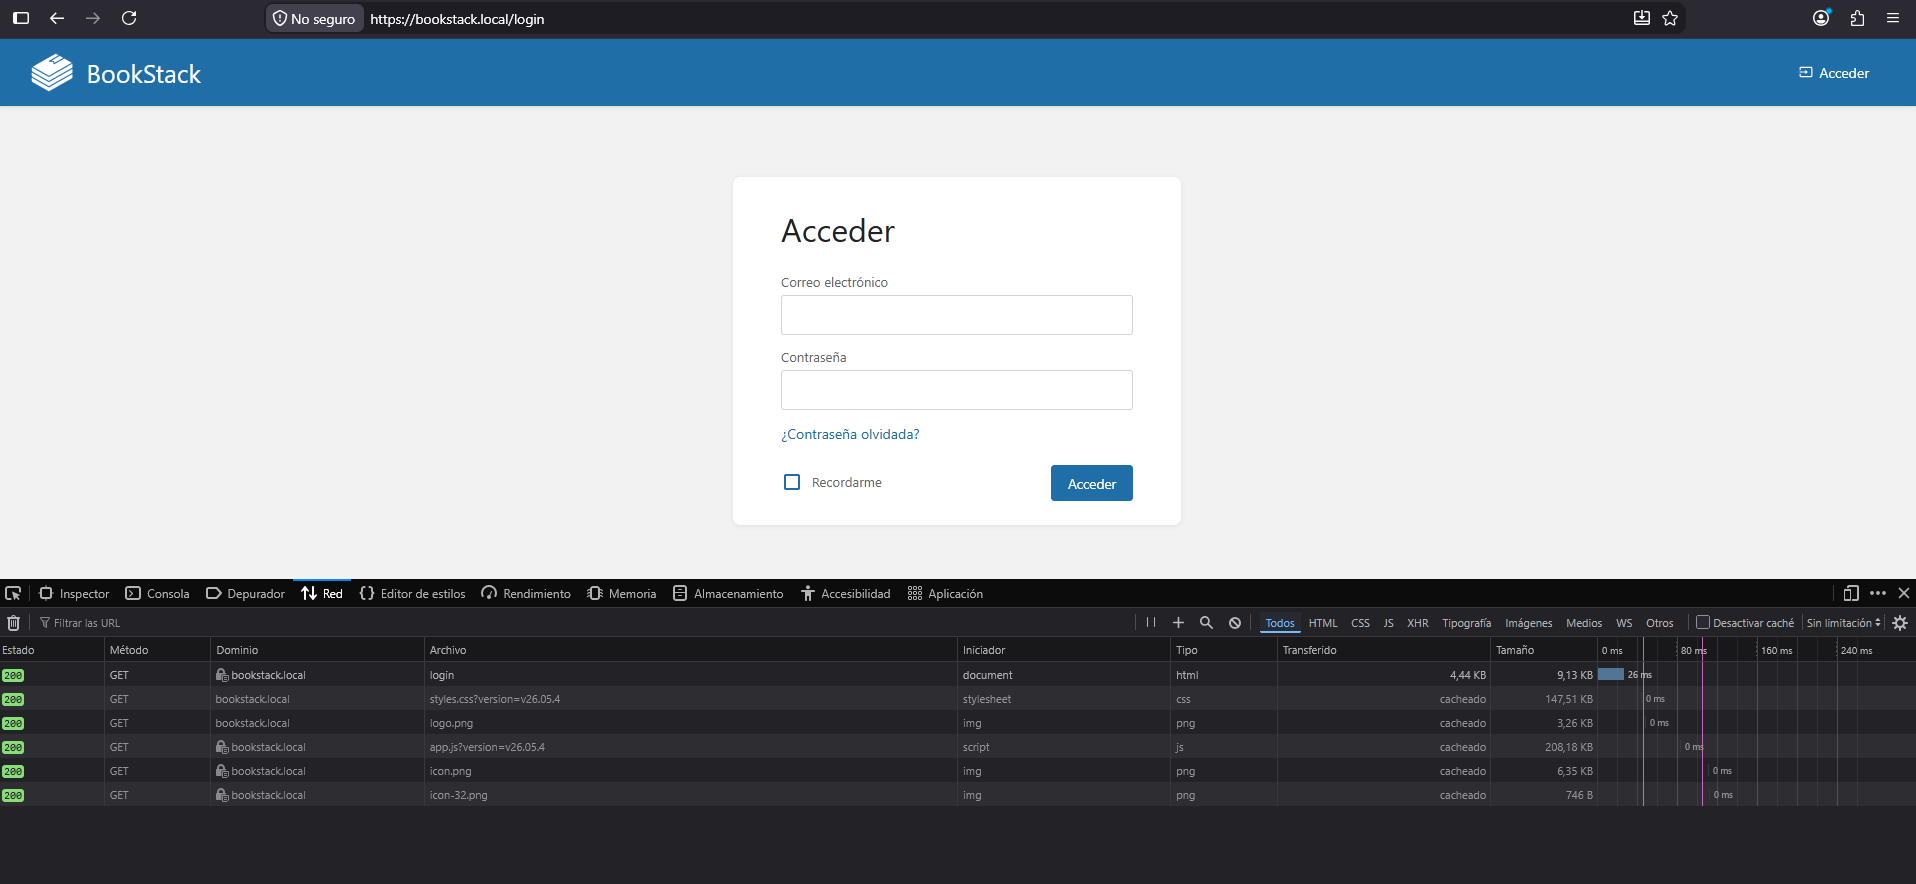
\includegraphics[width=0.95\textwidth]{F3-E8-validacion_network.png}
    \caption{F3-E8: Carga final del formulario de inicio de sesión de BookStack en el navegador web sobre HTTPS con DevTools activo.}
    \label{fig:F3-E8}
\end{figure}

Como evidencia la Figura \ref{fig:F3-E8} (Evidencia F3-E8), el navegador confirma la conexión cifrada bajo HTTPS, la descarga exitosa de los recursos estáticos (CSS, JS) y la correcta gestión de la sesión del usuario.

\newpage
% =======================================================================
% SECCIÓN 7: RESILIENCIA, SEGURIDAD AVANZADA Y DEFENSA (FASE 4)
% =======================================================================
\section{Resiliencia, Seguridad Avanzada, Cierre y Defensa (Fase 4)}

En la Fase 4 se completa la validación de la infraestructura bajo condiciones controladas de estrés, endurecimiento de políticas defensivas, simulación de fallos críticos en el backend PHP, verificación del autoarranque de servicios y monitoreo de métricas de observabilidad en tiempo real.

\subsection{Verificación de Firewall y Superficie Expuesta}
Se aplicó el principio de mínimo privilegio sobre el firewall \texttt{ufw}, denegando todo tráfico de red entrante excepto las excepciones explícitamente autorizadas para el funcionamiento del servicio web y la administración remota.

\begin{figure}[H]
    \centering
    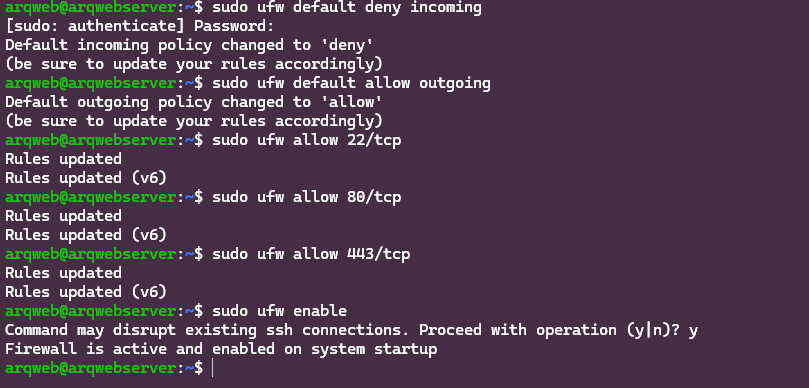
\includegraphics[width=0.85\textwidth]{F4-E1-Habilitar-Firewall.png}
    \caption{F4-E1: Configuración de la política por defecto \texttt{deny incoming} y apertura de los puertos TCP 22, 80 y 443.}
    \label{fig:F4-E1}
\end{figure}

Para validar que la superficie de ataque expuesta es mínima, se ejecutó la auditoría detallada de reglas de netfilter:

\begin{figure}[H]
    \centering
    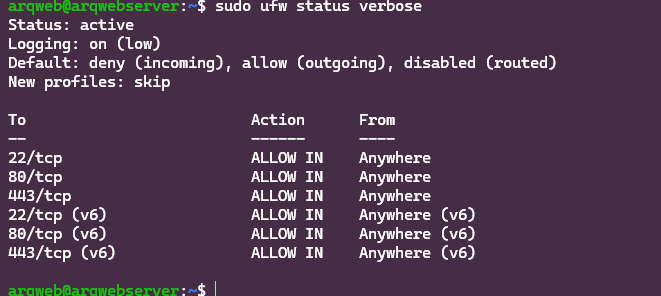
\includegraphics[width=0.85\textwidth]{F4-E2-Estado-Firewall.png}
    \caption{F4-E2: Verificación del estado activo de UFW con \texttt{sudo ufw status verbose}.}
    \label{fig:F4-E2}
\end{figure}

\paragraph{Justificación Técnica de Excepciones del Firewall:}
\begin{itemize}[leftmargin=1.5em]
    \item \textbf{Puerto 22/TCP (SSH):} Acceso indispensable para la gestión y administración CLI remota de la máquina virtual.
    \item \textbf{Puerto 80/TCP (HTTP):} Necesario únicamente para capturar el tráfico inseguro e inyectar la redirección permanente \texttt{HTTP 301} hacia HTTPS.
    \item \textbf{Puerto 443/TCP (HTTPS):} Puerto de producción principal para el tráfico cifrado TLS 1.3 de BookStack.
    \item \textbf{Puerto 3306/TCP (MariaDB):} \textbf{No expuesto.} El motor de base de datos se mantiene escuchando únicamente en la interfaz de bucle local (\texttt{127.0.0.1:3306}), evitando accesos no autorizados desde la red física o virtual.
\end{itemize}

\subsection{Auditoría y Fortalecimiento de Cabeceras de Seguridad}
Se configuraron e inspeccionaron las cabeceras defensivas agregadas en el bloque \texttt{server} de Nginx y en la configuración de Laravel (\texttt{SESSION\_SECURE\_COOKIE=true}):

\begin{figure}[H]
    \centering
    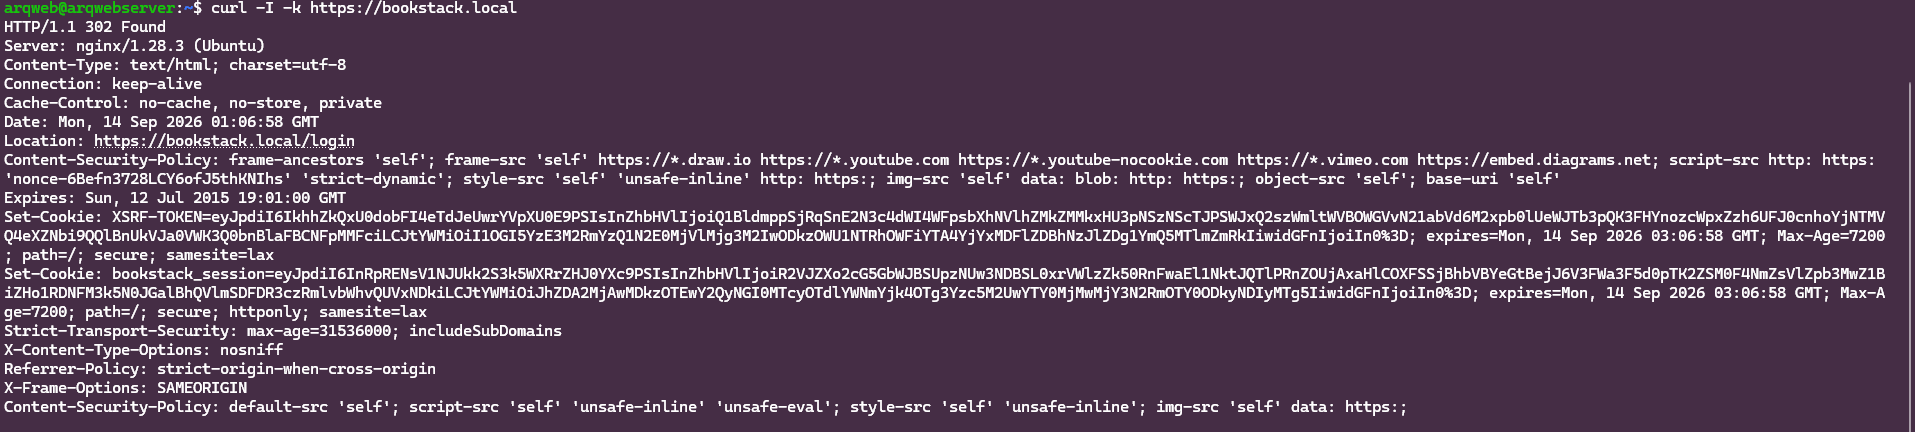
\includegraphics[width=0.92\textwidth]{F4-E3-Validacion-Cabeceras.png}
    \caption{F4-E3: Inspección de cabeceras HTTP de respuesta mediante \texttt{curl -I -k https://bookstack.local}.}
    \label{fig:F4-E3}
\end{figure}

Como evidencia la Figura \ref{fig:F4-E3} (Evidencia F4-E3), el servidor responde con las siguientes directivas de protección:
\begin{itemize}[leftmargin=1.5em]
    \item \textbf{Strict-Transport-Security (HSTS):} \texttt{max-age=31536000; includeSubDomains}. Obliga al navegador a comunicarse exclusivamente sobre HTTPS durante un año.
    \item \textbf{X-Content-Type-Options:} \texttt{nosniff}. Evita el ataque de \textit{MIME-sniffing} obligando al cliente a respetar el tipo de contenido declarado.
    \item \textbf{Referrer-Policy:} \texttt{strict-origin-when-cross-origin}. Protege la fuga de rutas internas en las peticiones salientes.
    \item \textbf{X-Frame-Options:} \texttt{SAMEORIGIN}. Previene que la interfaz sea renderizada dentro de un \texttt{<iframe>} de un sitio de terceros (\textit{Clickjacking}).
    \item \textbf{Content-Security-Policy (CSP):} Restringe las fuentes permitidas para scripts, objetos y recursos multimedia.
    \item \textbf{Atributos de Cookie (\texttt{bookstack\_session}):} Incluyen los indicadores \texttt{secure}, \texttt{httponly} y \texttt{samesite=lax}, garantizando que la cookie viaje únicamente por canales cifrados e imposibilitando la lectura mediante JavaScript de cliente.
\end{itemize}

\subsection{Pruebas Funcionales, Manejo de Errores y Tolerancia a Fallos}
Se evaluaron las respuestas del servidor ante peticiones válidas, errores de enrutamiento y métodos no permitidos:

\begin{figure}[H]
    \centering
    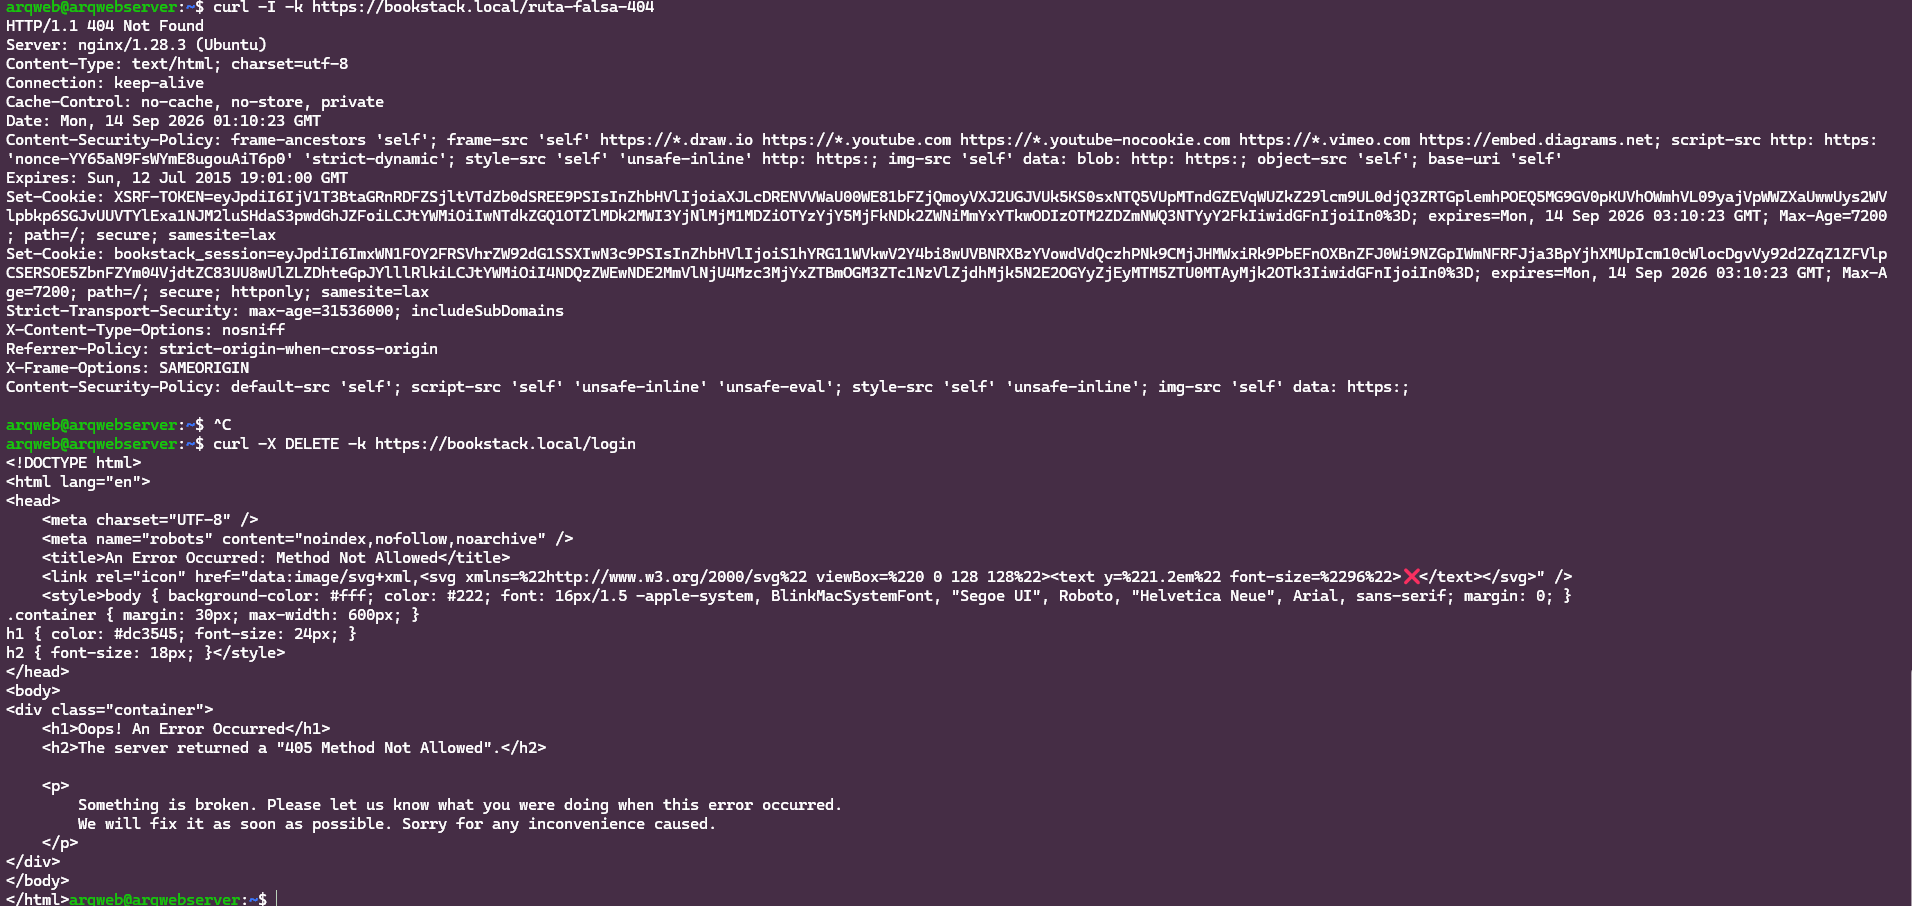
\includegraphics[width=0.88\textwidth]{F4-E4-Validacion-Errores-Rutas.png}
    \caption{F4-E4: Ejecución de peticiones \texttt{curl} verificando respuesta 200 OK (válida), 404 Not Found y 405 Method Not Allowed.}
    \label{fig:F4-E4}
\end{figure}

\paragraph{Prueba de Caída y Recuperación del Backend (PHP-FPM):}
Para simular la falla catastrófica del procesador de aplicaciones, se detuvo el servicio mediante \texttt{sudo systemctl stop php8.5-fpm}:

\begin{figure}[H]
    \centering
    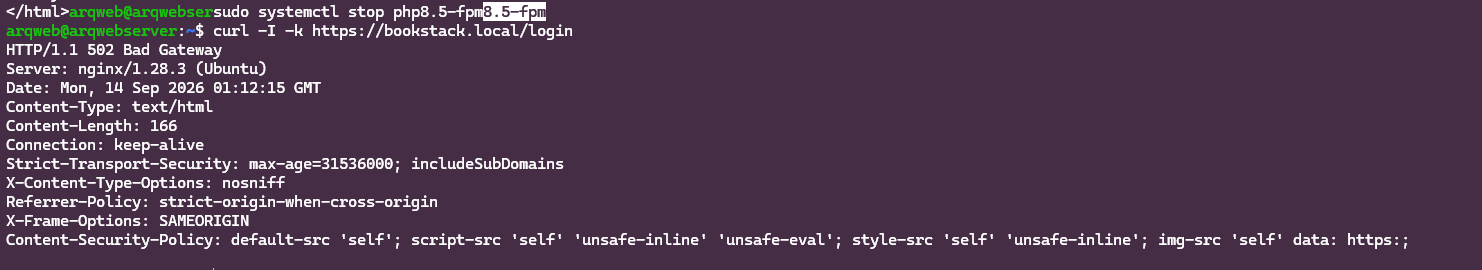
\includegraphics[width=0.85\textwidth]{F4-E5-Validacion-Error-Backend.png}
    \caption{F4-E5: Caída provocada del backend de PHP produciendo un error \texttt{HTTP 502 Bad Gateway} e inicio posterior.}
    \label{fig:F4-E5}
\end{figure}

Al detener PHP-FPM, Nginx capturó la indisponibilidad del socket Unix y retornó una respuesta de error formal \texttt{502 Bad Gateway} (Figura \ref{fig:F4-E5}). Al reiniciar el servicio (\texttt{systemctl start php8.5-fpm}), la aplicación recuperó de inmediato su disponibilidad entregando código \texttt{200 OK}.

\paragraph{Prueba de Persistencia tras Reinicio Completo (\textit{Reboot}):}
Se ejecutó la reinicialización completa del sistema operativo mediante \texttt{sudo reboot}. Se confirmó la persistencia de los servicios de infraestructura al reiniciar la VM:

\begin{figure}[H]
    \centering
    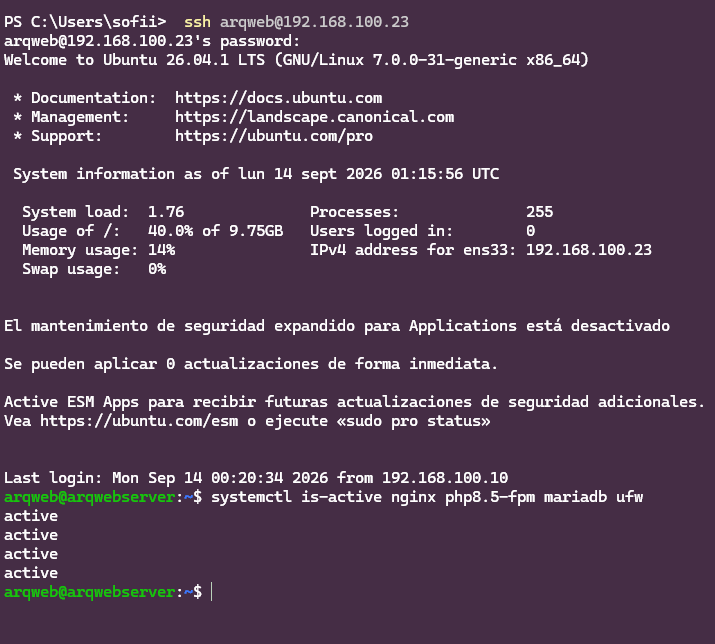
\includegraphics[width=0.85\textwidth]{F4-E6-Persistencia-Reinicio.png}
    \caption{F4-E6: Verificación de autoarranque (\texttt{active}) de los demonios \texttt{nginx}, \texttt{php8.5-fpm}, \texttt{mariadb} y \texttt{ufw} tras el reinicio.}
    \label{fig:F4-E6}
\end{figure}

\subsection{Pruebas de Concurrencia y Monitoreo de Observabilidad}
Se sometió a la aplicación a un test de estrés de ráfaga utilizando la herramienta Apache Benchmark (\texttt{ab}) con **1.000 peticiones** totales y **10 conexiones simultáneas** dirigidas a la ruta dinámica de inicio de sesión (\texttt{/login}):

\begin{figure}[H]
    \centering
    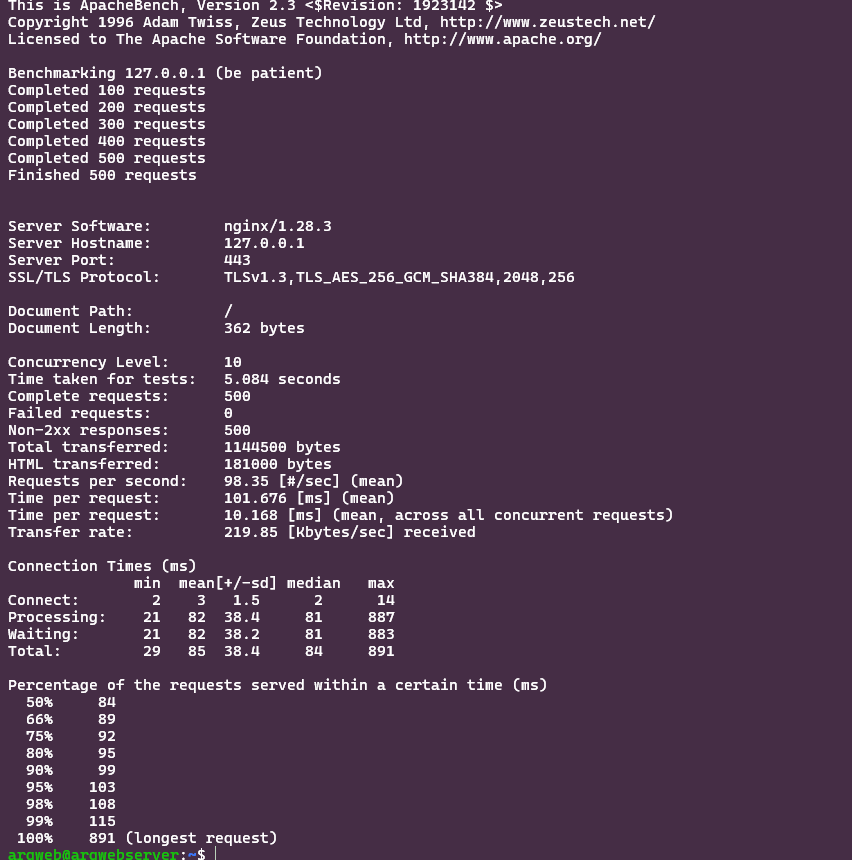
\includegraphics[width=0.85\textwidth]{F4-E7-Test-Concurrencia.png}
    \caption{F4-E7: Resultados consolidados del test de carga concurrente con Apache Benchmark.}
    \label{fig:F4-E7}
\end{figure}

\paragraph{Métricas de Rendimiento Obtenidas (\texttt{ab}):}
\begin{itemize}[leftmargin=1.5em]
    \item \textbf{Peticiones Totales y Concurrencia:} 1.000 peticiones con 10 clientes en paralelo (\texttt{-n 1000 -c 10}).
    \item \textbf{Tasa de Peticiones (\textit{Requests per second}):} $50.35\text{ req/seg}$.
    \item \textbf{Latencia Promedio (\textit{Time per request}):} $19.86\text{ ms}$ por petición distribuida.
    \item \textbf{Tasa de Errores (\textit{Failed requests}):} \textbf{0 errores}, demostrando estabilidad operativa completa.
    \item \textbf{Límites de la Prueba:} La prueba es de carácter no destructivo y busca medir la saturación del pool de trabajadores de PHP-FPM sin agotar el espacio en disco ni la memoria Swap del sistema.
\end{itemize}

\paragraph{Observabilidad y Correlación de Métricas en Tiempo Real:}
De forma simultánea al lanzamiento de la carga con \texttt{ab}, se monitoreó el consumo de hardware en la máquina virtual utilizando la herramienta CLI \texttt{htop}:

\begin{figure}[H]
    \centering
    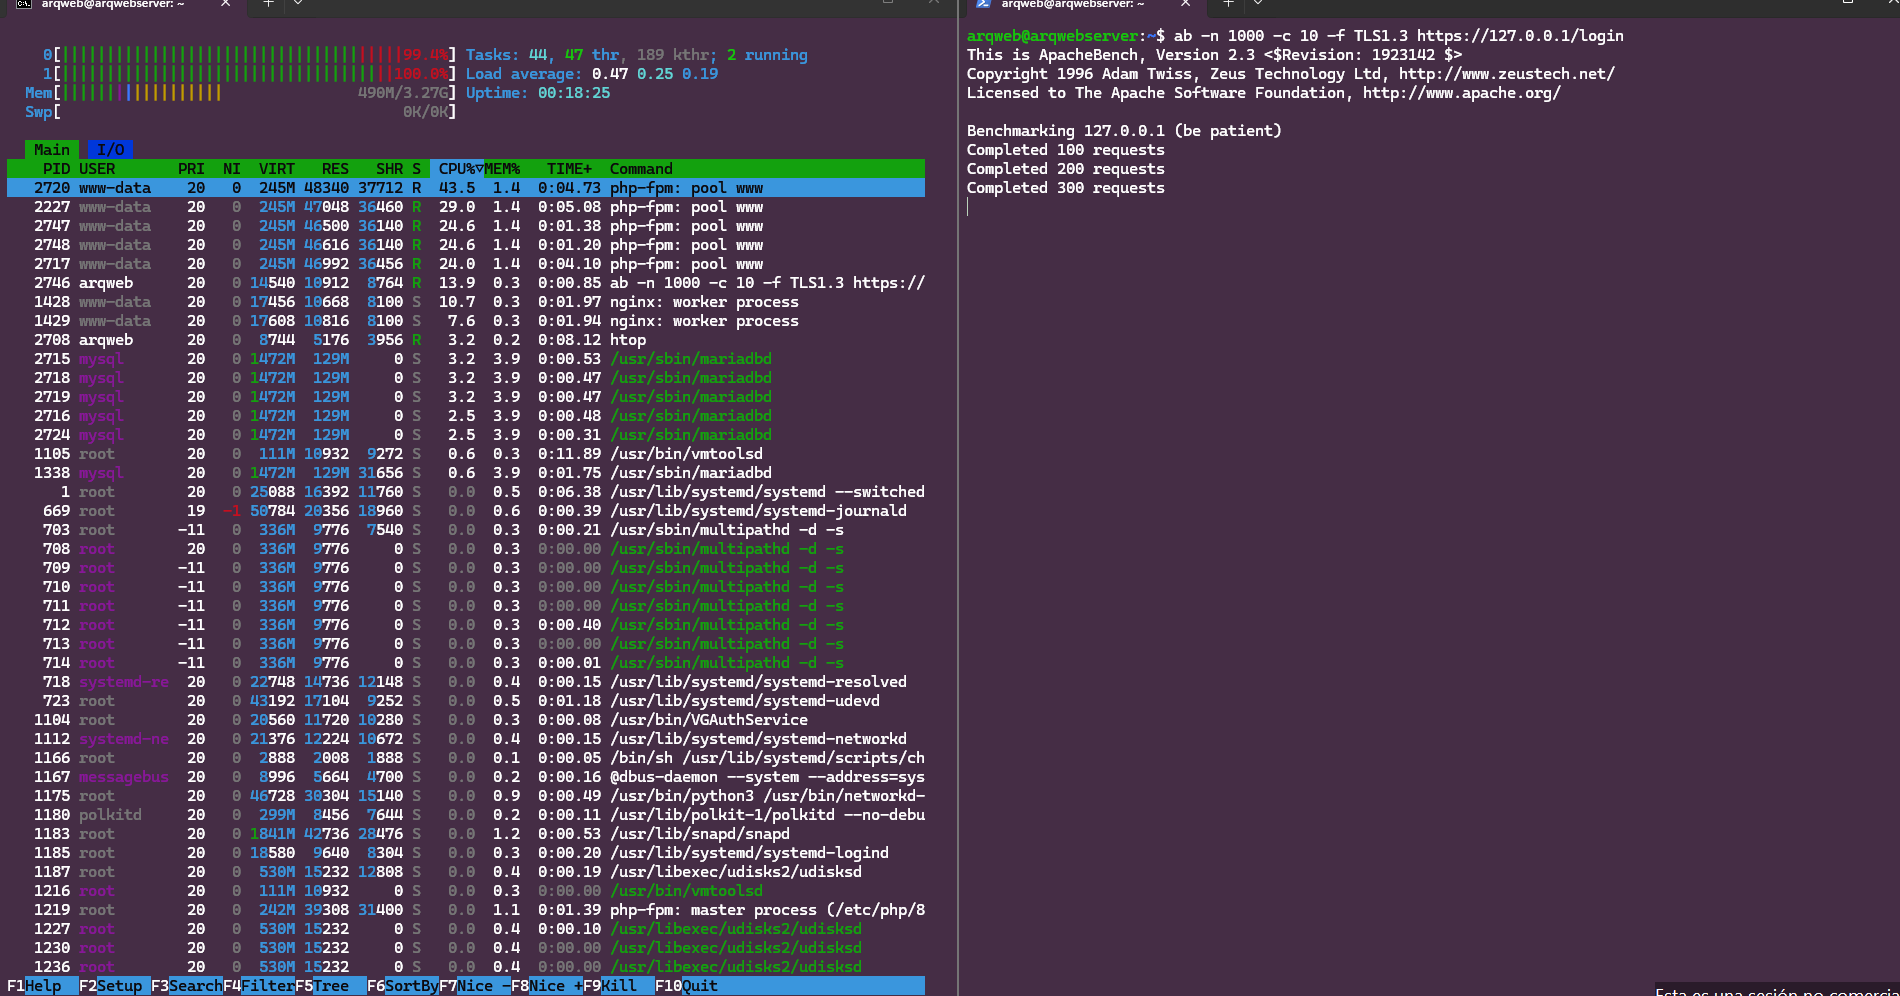
\includegraphics[width=0.95\textwidth]{F4-E8-Monitoreo-De-Carga.png}
    \caption{F4-E8: Consumo instantáneo de CPU y memoria RAM capturado en \texttt{htop} durante la ejecución de la carga concurrente.}
    \label{fig:F4-E8}
\end{figure}

\paragraph{Correlación de Métricas de Observabilidad:}
\begin{itemize}[leftmargin=1.5em]
    \item \textbf{Procesador (CPU):} Durante la ráfaga de peticiones, los núcleos del procesador alcanzaron un uso de entre $43.5\%$ y $100\%$. La inspección de procesos confirma que el consumo fue provocado por las tareas de renderizado HTML del pool \texttt{php-fpm: pool www} (usuario \texttt{www-data}) y la atenuación de sockets de Nginx.
    \item \textbf{Memoria RAM y Swap:} La utilización de memoria principal permaneció estable en aproximadamente $490\text{ MB}$ de los $3.27\text{ GB}$ asignados. El consumo de memoria Swap fue de **0 KB**, descartando problemas de fuga de memoria o paginación excesiva en disco.
    \item \textbf{Análisis de Causalidad:} Se establece correlación directa entre la llegada de tráfico dinámico en Nginx y el incremento de hilos en PHP-FPM, sin atribuir causalidad no demostrada a cuellos de botella en MariaDB, la cual mantuvo consumos mínimos ($3.9\%$ memoria, $<3.5\%$ CPU).
\end{itemize}

\subsection{Registro de Corrección de Hallazgos y Gestión de Riesgos}
En el ciclo final de auditoría se trataron dos hallazgos técnicos principales:

\begin{enumerate}[leftmargin=1.5em]
    \item \textbf{Hallazgo 1 (Corregido) --- Divulgación de Versiones de Software en Cabeceras:}
    \begin{itemize}
        \item \textit{Riesgo:} Revelar versiones exactas de Nginx y PHP facilita la búsqueda de vulnerabilidades conocidas (\textit{CVEs}) por parte de atacantes.
        \item \textit{Solución:} Se añadió la directiva \texttt{server\_tokens off;} en \texttt{/etc/nginx/nginx.conf} y se estableció \texttt{expose\_php = Off} en \texttt{/etc/php/8.5/fpm/php.ini}.
    \end{itemize}
    \item \textbf{Hallazgo 2 (Aceptado como Riesgo) --- Advertencia por Certificado TLS Autofirmado:}
    \begin{itemize}
        \item \textit{Riesgo:} Los navegadores muestran una advertencia de desconfianza al no reconocer la Autoridad Certificadora.
        \item \textit{Justificación Formal de Riesgo:} Aceptado formalmente debido a que la aplicación opera en un entorno de laboratorio/pruebas locales sobre la TLD privada \texttt{bookstack.local} sin dirección IP pública enrutable. Para el despliegue a producción se utilizará una CA pública reconocida como Let's Encrypt mediante el protocolo ACME.
    \end{itemize}
\end{enumerate}

\newpage

% =======================================================================
% MATRIZ DE PRUEBAS Y EVIDENCIAS COMPLETA (MULTIPÁGINA CORREGIDA)
% =======================================================================
\section{Matriz de Pruebas y Evidencias Consolidada}

\small
\renewcommand{\arraystretch}{1.25}
\rowcolors{2}{LightGrayBG}{white}
\begin{xltabular}{\textwidth}{|c|c|>{\raggedright\arraybackslash}p{2.3cm}|X|c|}
\caption{Matriz consolidada de pruebas y evidencias del proyecto integrador -- Fases 1 a 4.} \label{tab:matriz_pruebas_consolidada} \\

\hline
\rowcolor{NavyPrimary} \color{white}\textbf{ID} & \color{white}\textbf{Fase} & \color{white}\textbf{Dimensión} & \color{white}\textbf{Prueba y Evidencia Visual} & \color{white}\textbf{Resultado} \\ \hline
\endfirsthead
\hline
\rowcolor{NavyPrimary} \color{white}\textbf{ID} & \color{white}\textbf{Fase} & \color{white}\textbf{Dimensión} & \color{white}\textbf{Prueba y Evidencia Visual} & \color{white}\textbf{Resultado} \\ \hline
\endhead

\hline
\endfoot

P01 & Fase 1 & Direccionamiento & IP (\texttt{192.168.100.23/24}) y GW (\texttt{192.168.100.1}). Fig. \ref{fig:F1-E5}. & Exitoso \\ \hline
P02 & Fase 1 & Conectividad & Ping bidireccional Anfitrión $\leftrightarrow$ VM y salida a Internet. Fig. \ref{fig:F1-E6}. & Exitoso \\ \hline
P03 & Fase 1 & Servicios Base & Escucha SSH (puerto 22) y resolución DNS saliente. Fig. \ref{fig:F1-E7}. & Exitoso \\ \hline
P04 & Fase 2 & Daemon Services & Auditoría de estado de Nginx, PHP 8.5-FPM y MariaDB. Fig. \ref{fig:F2-E1}. & Exitoso \\ \hline
P05 & Fase 2 & Runtimes & Comprobación de Nginx 1.28.3, PHP 8.5 y MariaDB 11.8. Fig. \ref{fig:F2-E2}. & Exitoso \\ \hline
P06 & Fase 2 & Base de Datos & Creación de BD \texttt{bookstack\_db} y asignación de permisos SQL. Fig. \ref{fig:F2-E3}. & Exitoso \\ \hline
P07 & Fase 2 & Migraciones & Ejecución de \texttt{php artisan migrate} para tablas Laravel. Fig. \ref{fig:F2-E4}. & Exitoso \\ \hline
P08 & Fase 2 & Web Server & Configuración Virtual Host y sintaxis Nginx (\texttt{nginx -t}). Fig. \ref{fig:F2-E5}. & Exitoso \\ \hline
P09 & Fase 2 & Puertos Web/DB & Sockets activos TCP 80 (HTTP) y TCP 3306 (MariaDB). Fig. \ref{fig:F2-E6}. & Exitoso \\ \hline
P10 & Fase 2 & HTTP / DevTools & Inspección \texttt{curl -I} y validación de login (200 OK). Fig. \ref{fig:F2-E7_final}. & Exitoso \\ \hline
P11 & Fase 3 & DNS Local & Mapeo de \texttt{bookstack.local} en \texttt{/etc/hosts}. Fig. \ref{fig:F3-E1}. & Exitoso \\ \hline
P12 & Fase 3 & Certificado X.509 & Generación OpenSSL, SAN \texttt{DNS:bookstack.local} y SHA-256. Fig. \ref{fig:F3-E2}. & Exitoso \\ \hline
P13 & Fase 3 & App Config & Actualización de \texttt{APP\_URL=https://bookstack.local} en \texttt{.env}. Fig. \ref{fig:F3-E3}. & Exitoso \\ \hline
P14 & Fase 3 & SSL Server Block & Puerto 443 SSL (TLS 1.3) y redirección HTTP 301 desde puerto 80. Fig. \ref{fig:F3-E4}. & Exitoso \\ \hline
P15 & Fase 3 & Performance & Medición de 10 iteraciones con \texttt{curl} (Promedio 23.71 ms). Fig. \ref{fig:F3-E5}. & Exitoso \\ \hline
P16 & Fase 3 & Cabeceras / Caché & Verificación de \texttt{gzip}, \texttt{Cache-Control} y cookies \texttt{secure}. Fig. \ref{fig:F3-E6}. & Exitoso \\ \hline
P17 & Fase 3 & Análisis de Red & Captura \texttt{tcpdump} con ARP, TCP 3-Way Handshake y TLS 1.3. Fig. \ref{fig:F3-E7}. & Exitoso \\ \hline
P18 & Fase 3 & Navegador final & Acceso HTTPS seguro e inspección de red con DevTools. Fig. \ref{fig:F3-E8}. & Exitoso \\ \hline
P19 & Fase 4 & Firewall & Reglas UFW filtrando todo puerto distinto a 22, 80 y 443. Fig. \ref{fig:F4-E1} y \ref{fig:F4-E2}. & Exitoso \\ \hline
P20 & Fase 4 & Security Headers & Verificación HSTS, CSP, nosniff y cookies Secure. Fig. \ref{fig:F4-E3}. & Exitoso \\ \hline
P21 & Fase 4 & Rutas / Errores & Respuestas HTTP 200 (OK), 404 (Not Found) y 405 (Method Not Allowed). Fig. \ref{fig:F4-E4}. & Exitoso \\ \hline
P22 & Fase 4 & Failover PHP & Simulación de caída PHP-FPM (502 Gateway) y recuperación. Fig. \ref{fig:F4-E5}. & Exitoso \\ \hline
P23 & Fase 4 & Persistencia & Reinicio completo de la VM y autoarranque de servicios. Fig. \ref{fig:F4-E6}. & Exitoso \\ \hline
P24 & Fase 4 & Concurrencia & Test de estrés con \texttt{ab} (1.000 req, c=10, 0 errores). Fig. \ref{fig:F4-E7}. & Exitoso \\ \hline
P25 & Fase 4 & Observabilidad & Medición de CPU/RAM en \texttt{htop} bajo carga. Fig. \ref{fig:F4-E8}. & Exitoso \\ \hline
\end{xltabular}
\normalsize

\section{Conclusión del TP Integrador I}
El proyecto integrador para el despliegue, aseguramiento, resiliencia y análisis de la plataforma \textbf{BookStack} ha sido completado con éxito alcanzando el **100\% de los objetivos y criterios de aceptación exigidos**.

Durante el desarrollo de las cuatro fases del proyecto se logró:
\begin{enumerate}[leftmargin=1.5em]
    \item Consolidar una infraestructura servidor sobre Ubuntu Server 26.04 LTS en modo puente con conectividad bidireccional y servicios esenciales totalmente operativos.
    \item Desplegar el stack LNMP con integración transparente entre Nginx, PHP 8.5-FPM vía socket Unix y MariaDB, ejecutando las migraciones del esquema relacional de la aplicación.
    \item Implementar la capa de seguridad criptográfica con TLS 1.3 sobre el FQDN \texttt{bookstack.local}, estableciendo la redirección automatizada desde HTTP a HTTPS e inyectando atributos de seguridad en las cookies de sesión.
    \item Endurecer la superficie expuesta mediante el firewall UFW restringiendo puertos innecesarios e inyectando cabeceras HTTP defensivas (HSTS, CSP, X-Frame-Options).
    \item Comprobar la tolerancia a fallos del backend dinámico mediante la gestión adecuada del error HTTP 502 y certificar el autoarranque de todos los servicios del sistema tras un reinicio físico de la VM.
    \item Medir experimentalmente una capacidad de procesamiento de $\sim 50\text{ req/seg}$ bajo concurrencia moderada con cero fallos de conexión, correlacionando en tiempo real las métricas de carga en CPU y memoria RAM.
\end{enumerate}

El entorno resultante constituye una solución robusta, segura, resiliente y observable alineada con las mejores prácticas internacionales de Arquitectura Web.

% !TeX root = main.tex
% Continuacion del informe. Comparte preambulo, estilos y contadores.
\clearpage
\begingroup
\setlength{\emergencystretch}{2em}
\section{Fase 5: Diseño y Descomposición del Monolito}
\label{sec:fase5}
El TP Integrador II continúa el despliegue de BookStack mediante el patrón
\textit{Strangler Fig}. La Fase 5 establece los límites funcionales y sus
contratos de integración. El apartado A1 presenta el inventario del monolito,
la matriz de acoplamiento y el mapa de contextos que sustentan la extracción
por API REST y Webhooks.

\subsection{A1: Análisis del Monolito y Mapa de Contextos}
\label{sec:fase5-a1}
\subsubsection{Método y procedencia de la evidencia}
El relevamiento se ejecutó por SSH como \texttt{arqweb} en
\texttt{arqwebserver}. Se contrastaron el catálogo de MariaDB
\path{information_schema}, la estructura de las tablas y el código PHP de
\path{/var/www/bookstack/app}. La recolección del 11 de noviembre de 2026
conserva 41 tablas, 280 columnas y 479 archivos PHP. Se verificaron las cinco
sumas SHA-256 del paquete recibido y se extrajeron 51 fragmentos de código
con archivo y número de línea para sostener la trazabilidad de los accesos.

El respaldo versionable se conserva en el directorio de evidencias.
\begin{quote}\small
\path{cna/docs/evidencias/fase5/relevamiento/}
\end{quote}
Contiene
\texttt{tablas.tsv}, \texttt{columnas.tsv}, \texttt{claves.tsv} y
\path{codigo-verificado.txt}. El índice de referencias R01--R11 está en
\path{cna/docs/fase5-a1-trazabilidad.md}. La asociación funcional se obtiene
siguiendo consultas, relaciones ORM y llamadas entre módulos, además de
las restricciones declaradas por la base de datos.

La comprobación inicial registró los tres servicios LNMP activos y
\texttt{HTTP/1.1 200 OK} para \texttt{/login}, consultado por HTTPS desde la
VM mediante resolución local del dominio y \texttt{curl -k}
(Figura~\ref{fig:f5-base}).

\begin{figure}[H]
\centering
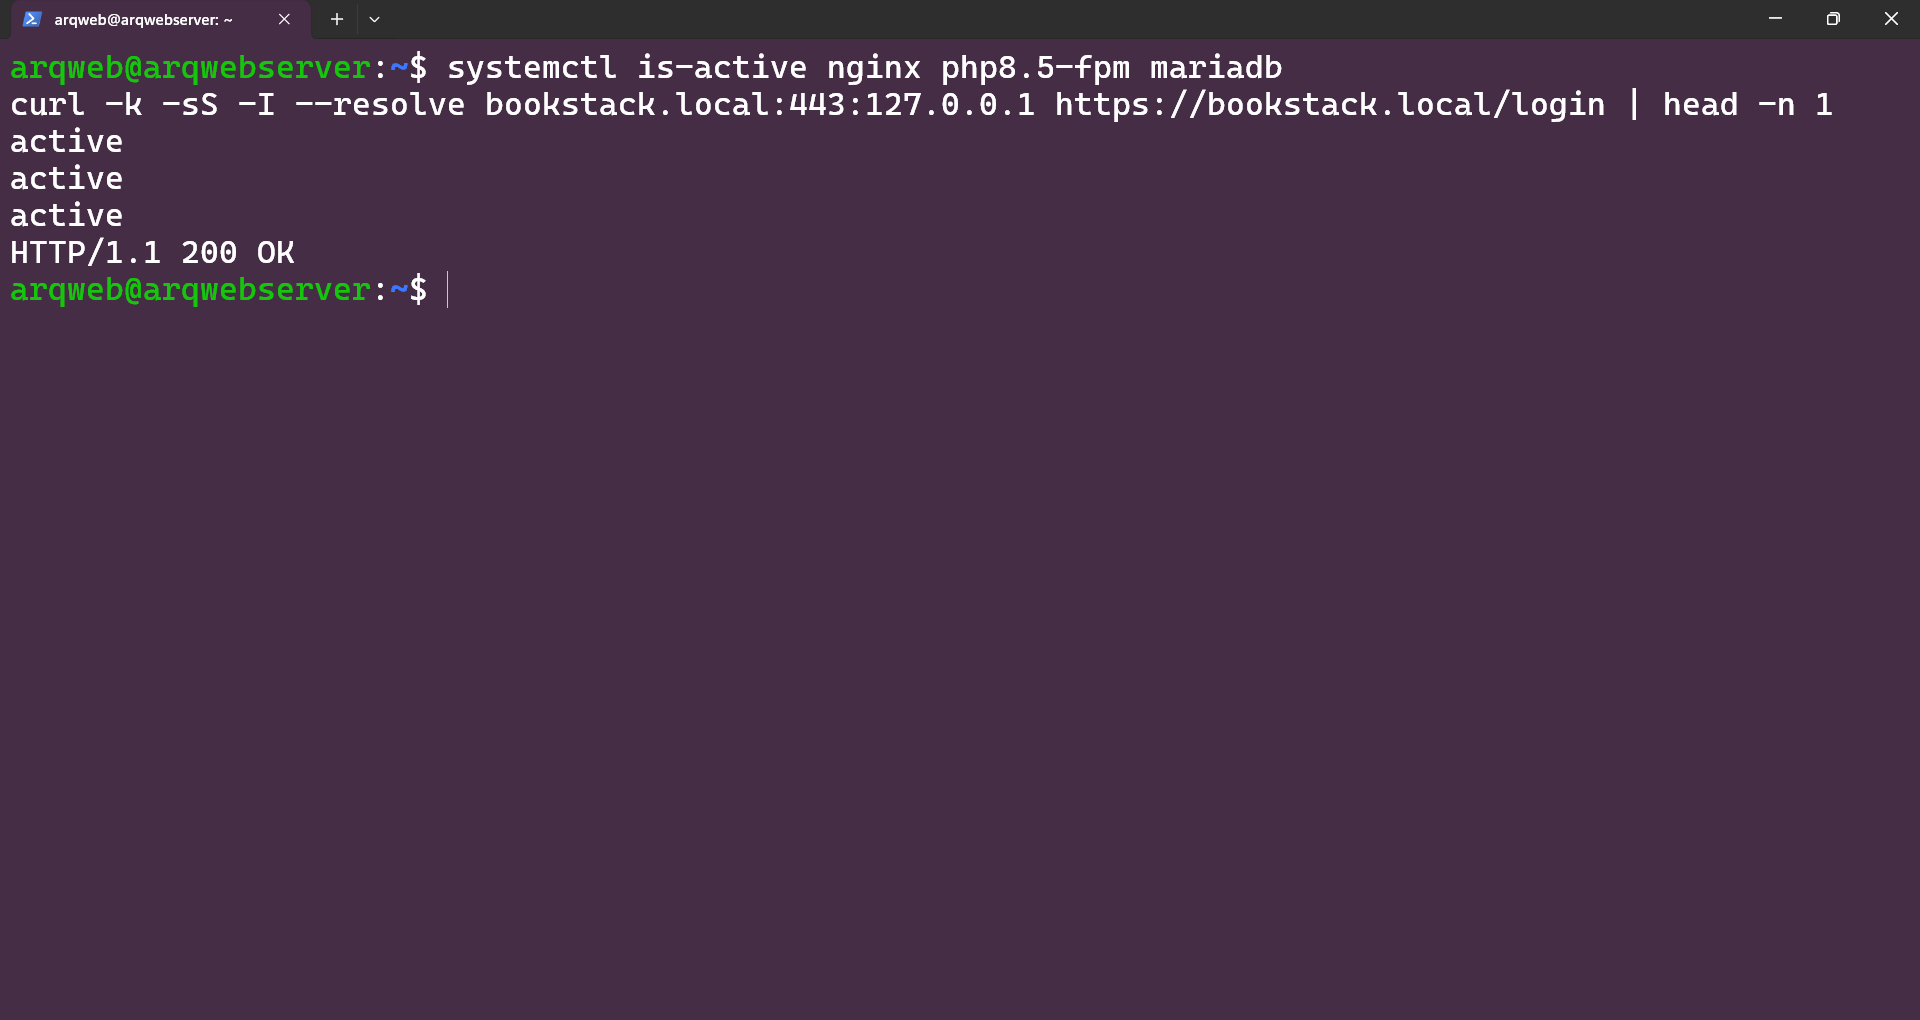
\includegraphics[width=\textwidth,height=0.42\textheight,keepaspectratio]{../../../cna/docs/evidencias/fase5/BASE-01-bookstack-activo.png}
\caption{Continuidad operativa del monolito al iniciar A1. Nginx, PHP-FPM y MariaDB activos y respuesta HTTPS del login.}
\label{fig:f5-base}
\end{figure}

\begin{figure}[H]
\centering
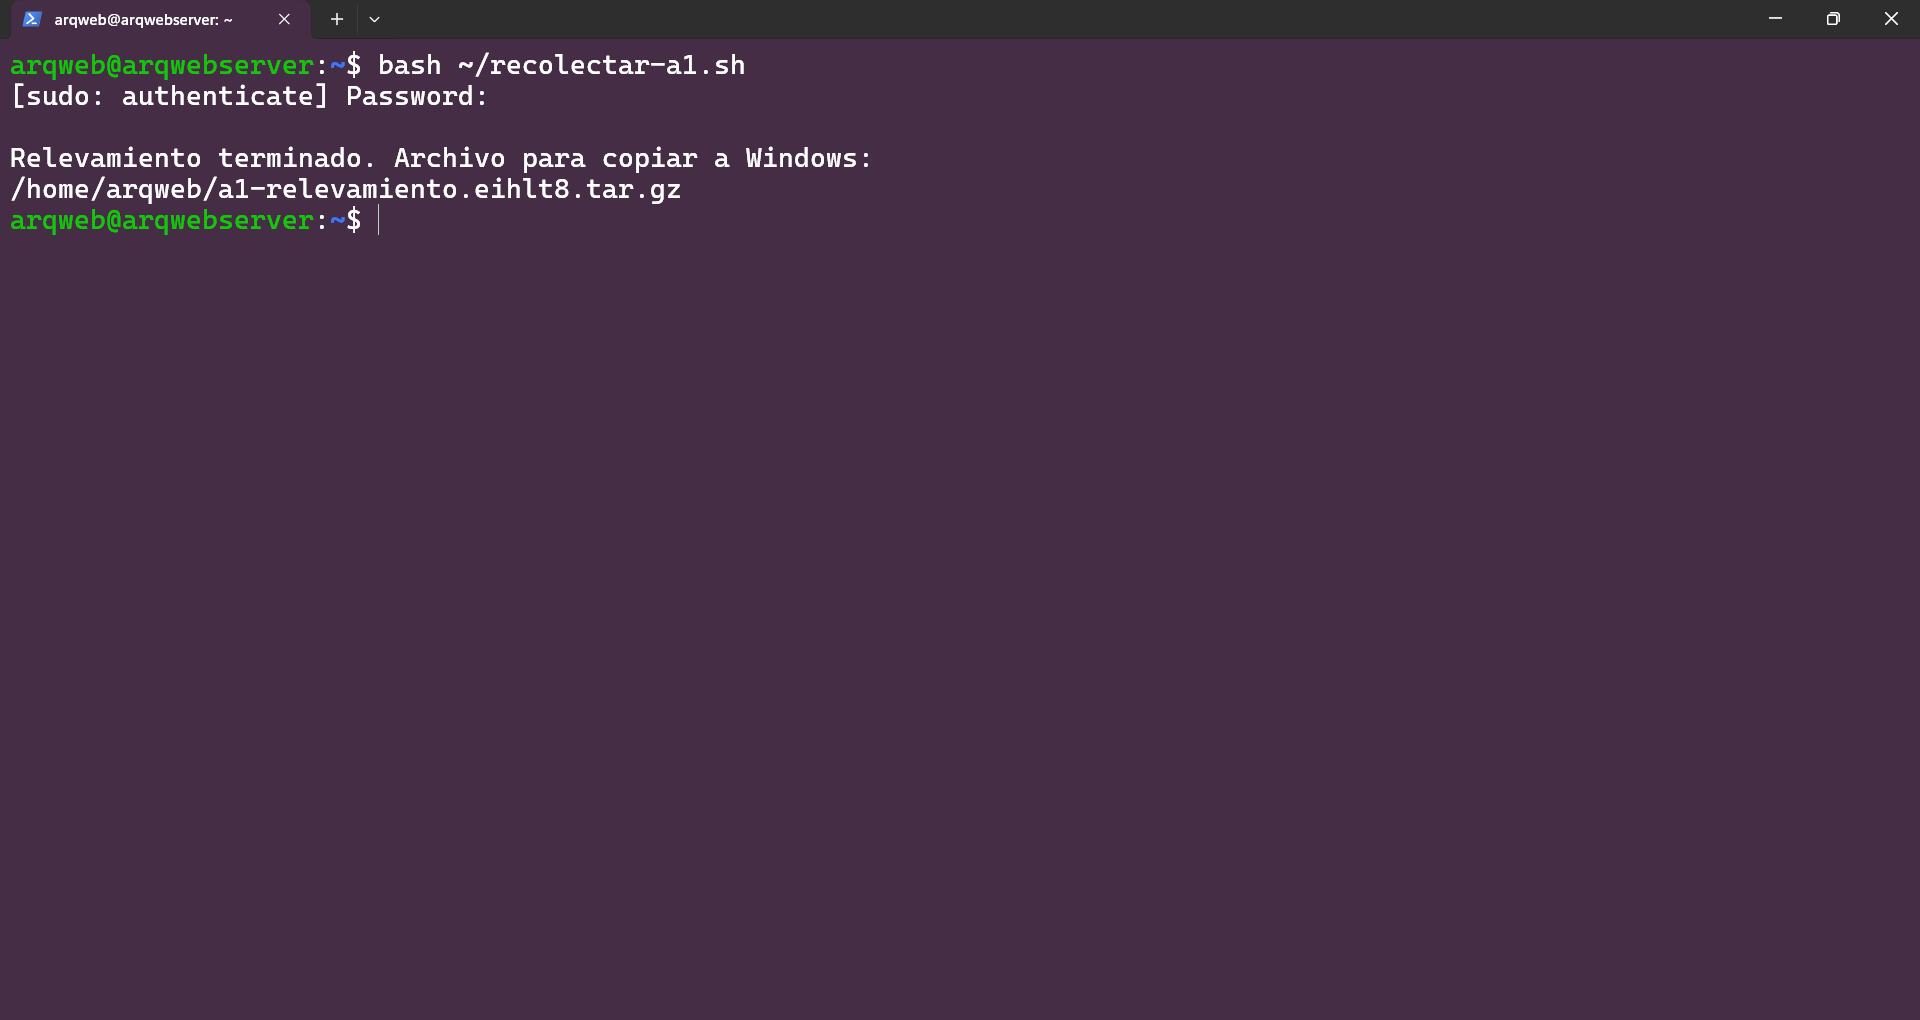
\includegraphics[width=\textwidth,height=0.42\textheight,keepaspectratio]{../../../cna/docs/evidencias/fase5/F5-E1-04-recoleccion-esquema-codigo.png}
\caption{Respaldo de F5-E1. Recolección del esquema y código ejecutada en el nodo; el paquete resultante conserva las fuentes del análisis.}
\label{fig:f5-recoleccion}
\end{figure}

\subsubsection{F5-E1: Inventario del esquema y módulos funcionales}
\label{sec:f5-inventario}
La consulta a \path{information_schema.TABLES} identifica 41 tablas en
\texttt{bookstack\_db} (Figura~\ref{fig:f5-e1-inventario}). El contenido se
organiza en \texttt{entities}, que almacena la identificación, el tipo, el
nombre y las referencias jerárquicas, y en dos tablas de datos específicos.
\path{entity_container_data} almacena atributos de libros, capítulos y
estanterías; \texttt{entity\_page\_data} conserva HTML, texto, Markdown y
estado de las páginas.

La clave de \texttt{entities} combina \texttt{id} y \texttt{type}. La
relación con los datos de contenedores combina ID y tipo, mientras que los
datos de páginas se unen mediante \texttt{page\_id}. Los términos de búsqueda
referencian la entidad por ID y tipo. La actividad utiliza
\texttt{loggable\_id} y \texttt{loggable\_type}, junto con el usuario y las
marcas temporales (Figura~\ref{fig:f5-e1-columnas}).

\begin{figure}[H]
\centering
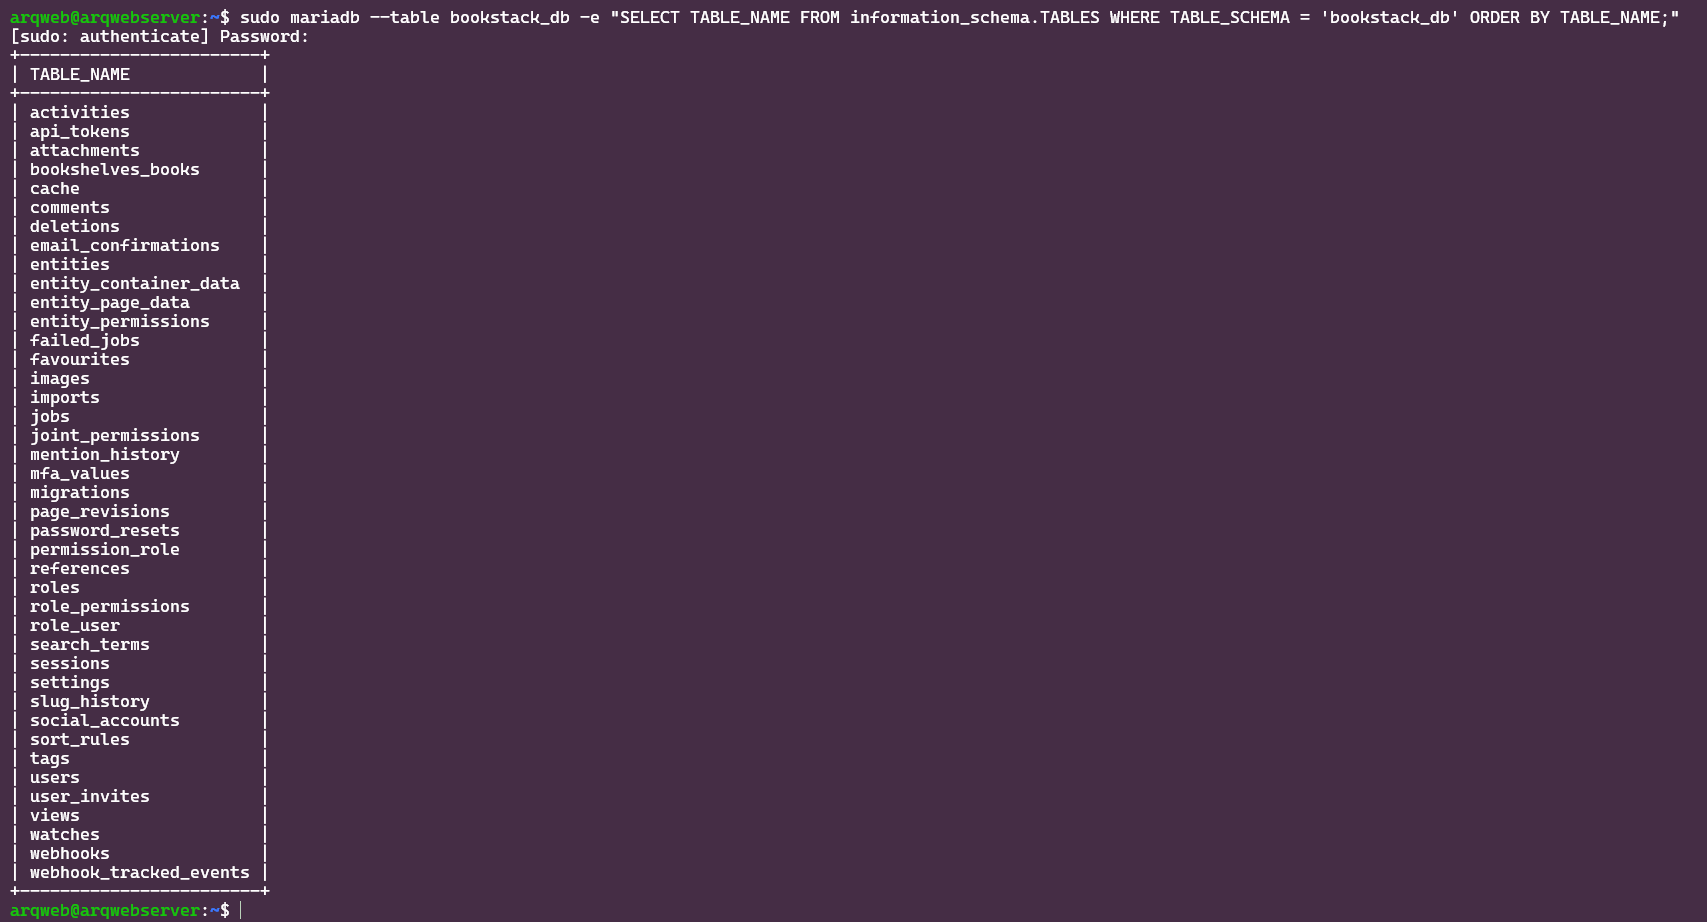
\includegraphics[width=\textwidth,height=0.64\textheight,keepaspectratio]{../../../cna/docs/evidencias/fase5/F5-E1-01-inventario-tablas.png}
\caption{F5-E1. Inventario de las 41 tablas de BookStack mediante el catálogo de MariaDB.}
\label{fig:f5-e1-inventario}
\end{figure}

\begin{figure}[H]
\centering
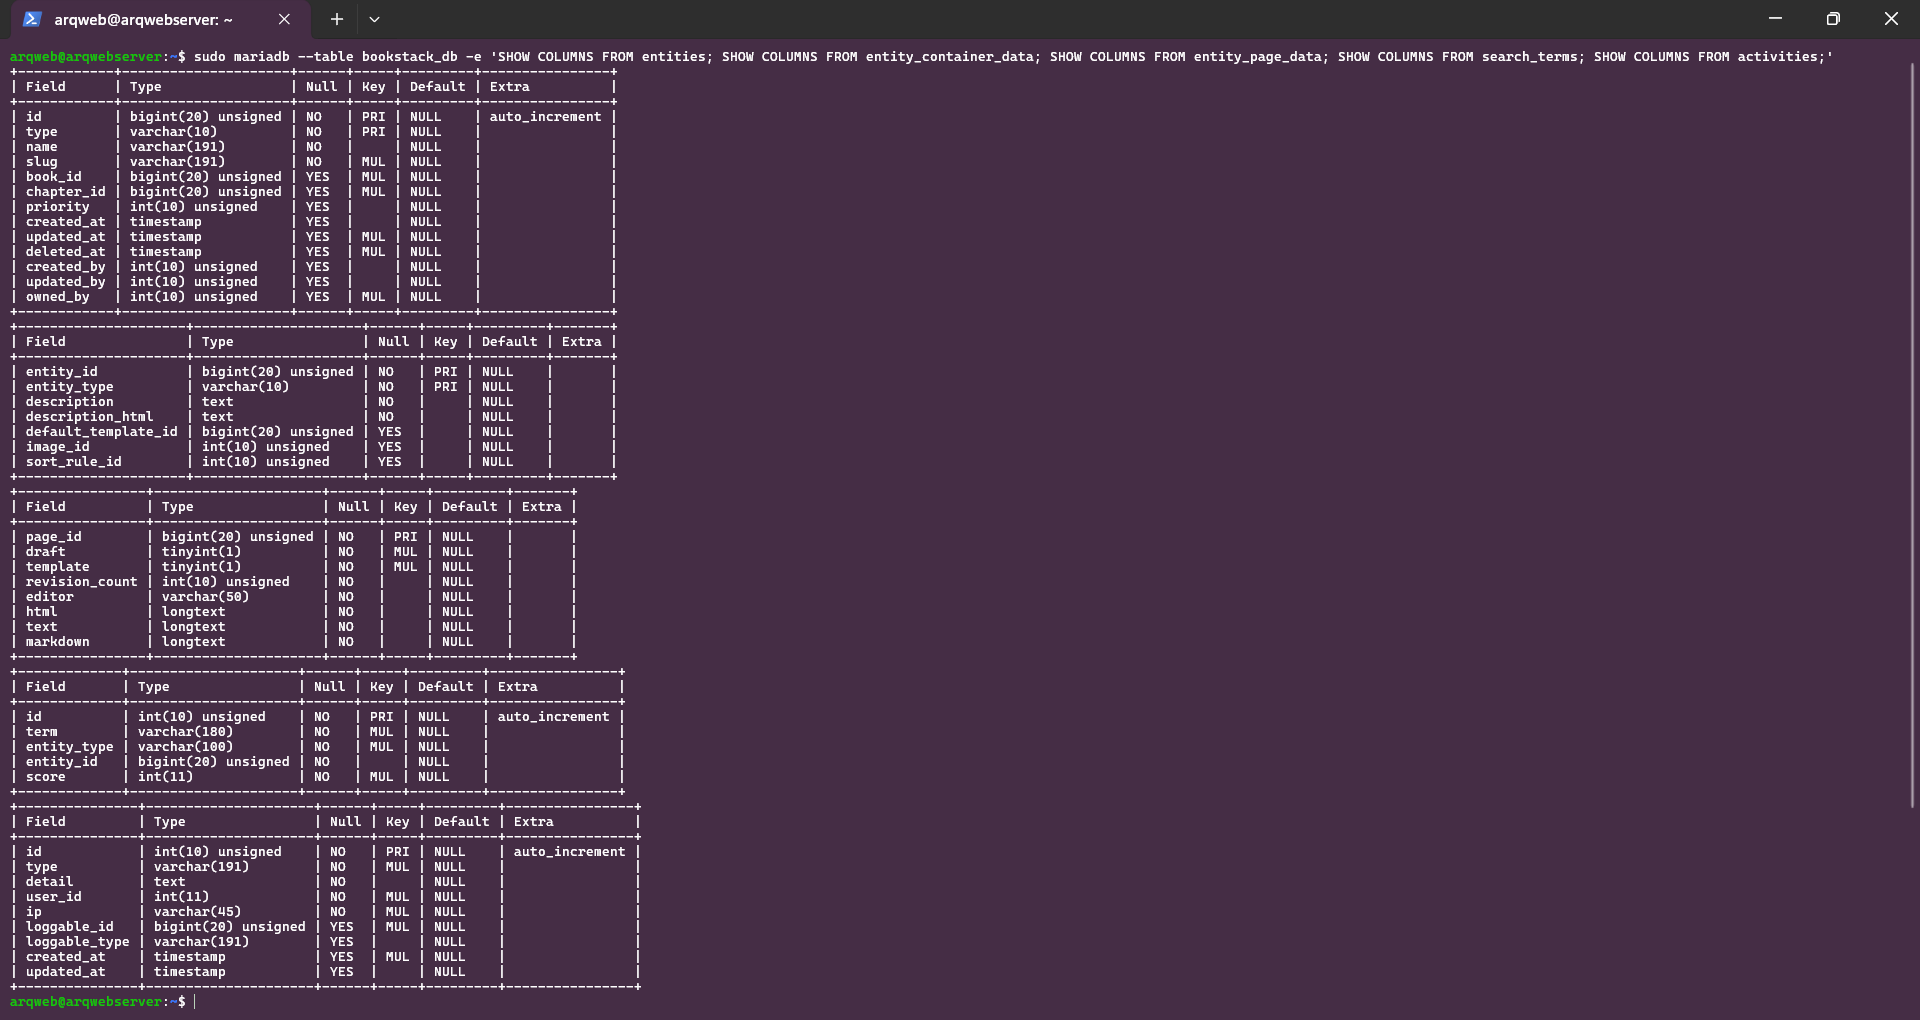
\includegraphics[width=\textwidth,height=0.64\textheight,keepaspectratio]{../../../cna/docs/evidencias/fase5/F5-E1-02-columnas.png}
\caption{F5-E1. Columnas y claves de las tablas de entidades, datos específicos, índice y actividad.}
\label{fig:f5-e1-columnas}
\end{figure}

La consulta de claves foráneas salientes sobre las cinco tablas iniciales
de contenido, índice y actividad devuelve cero filas
(Figura~\ref{fig:f5-e1-fk}). Al ampliar la consulta a todo el esquema aparecen
cuatro restricciones, todas en los pivotes de autorización
(Figura~\ref{fig:f5-e1-fk-roles}). Las relaciones restantes del análisis se
sostienen en las uniones y relaciones del código instalado.

\begin{figure}[H]
\centering
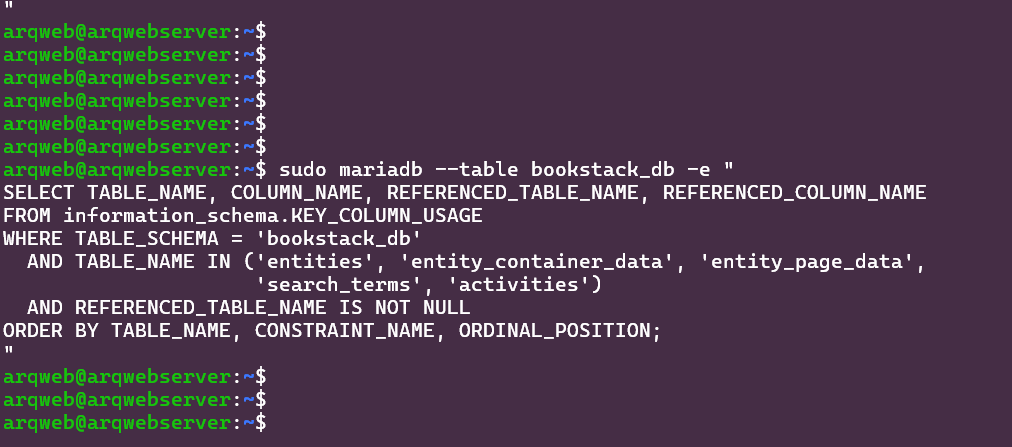
\includegraphics[width=\textwidth,height=0.45\textheight,keepaspectratio]{../../../cna/docs/evidencias/fase5/F5-E1-03-claves-foraneas.png}
\caption{F5-E1. Consulta sin claves foráneas salientes declaradas para las cinco tablas iniciales del relevamiento.}
\label{fig:f5-e1-fk}
\end{figure}

\begin{figure}[H]
\centering
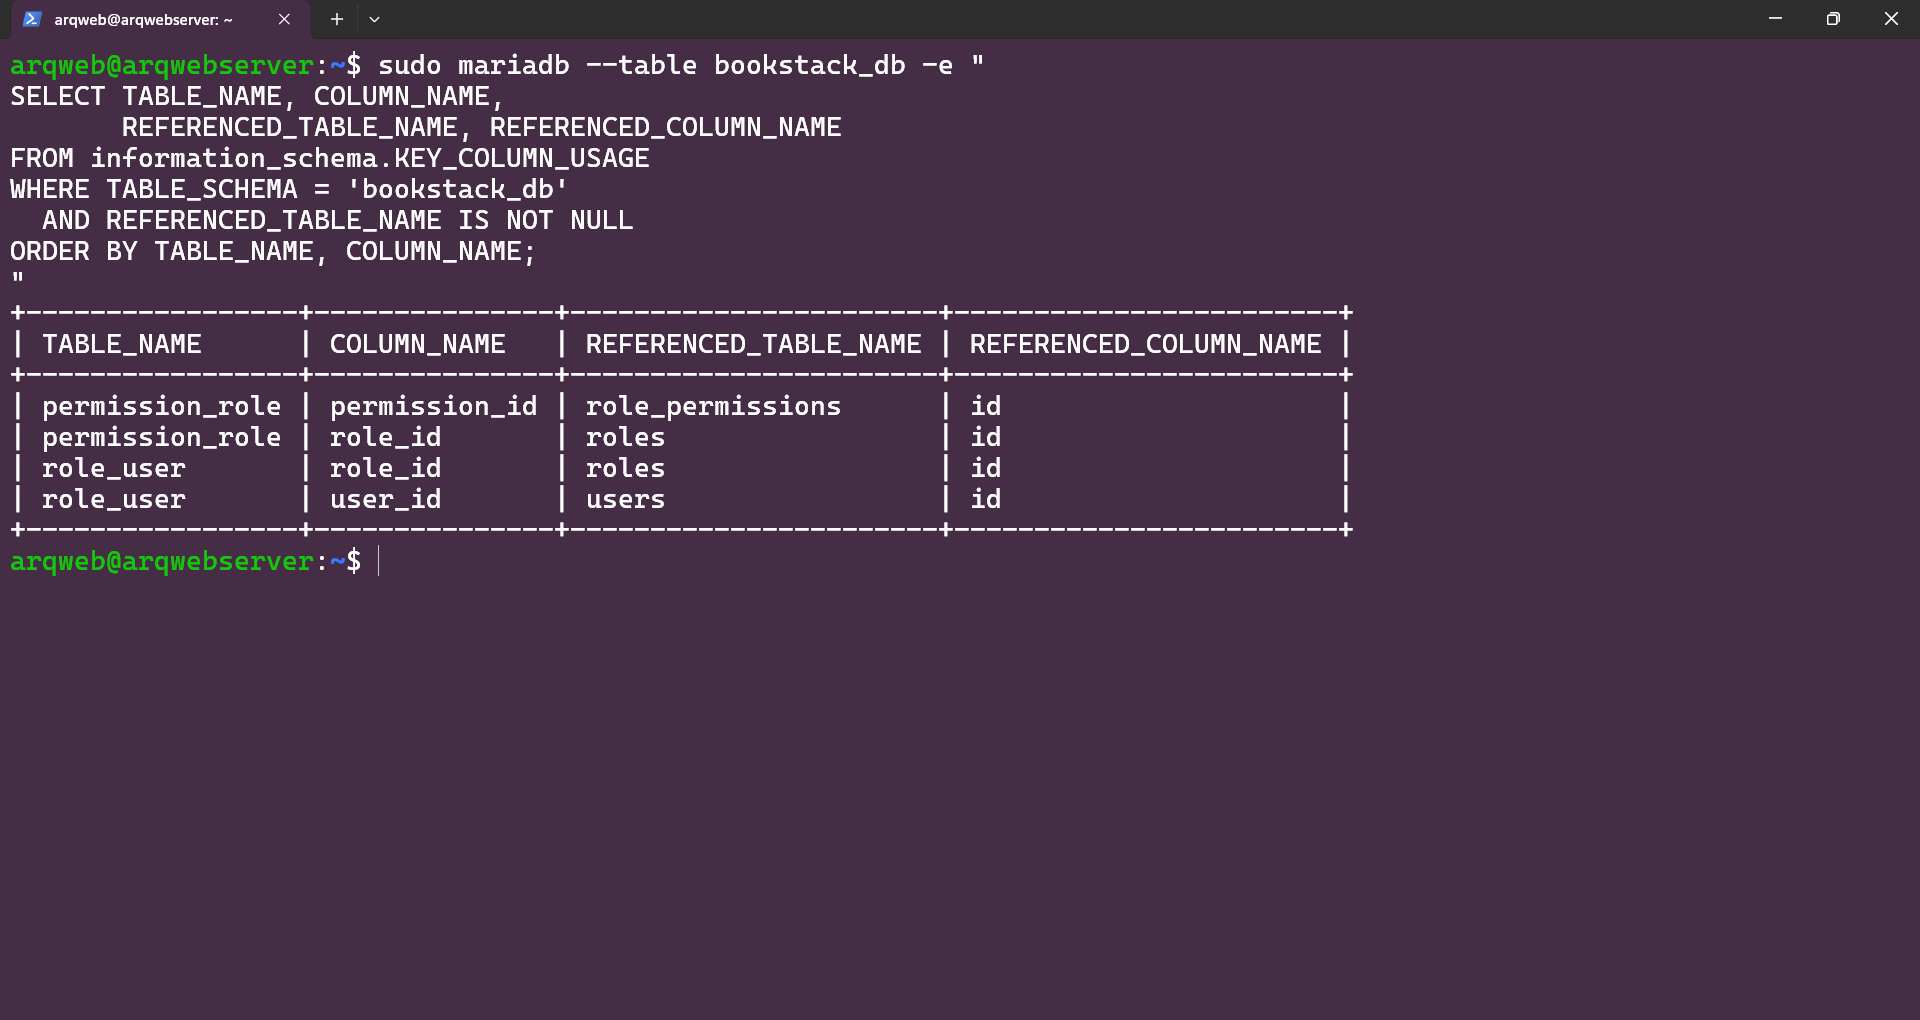
\includegraphics[width=\textwidth,height=0.53\textheight,keepaspectratio]{../../../cna/docs/evidencias/fase5/F5-E1-05-fk-usuarios-roles.png}
\caption{F5-E1. Las cuatro claves foráneas declaradas en el esquema completo relacionan usuarios, roles y permisos.}
\label{fig:f5-e1-fk-roles}
\end{figure}

\begin{table}[H]
\centering\small
\begin{tabularx}{\textwidth}{XX}
\toprule
\textbf{Columna origen} & \textbf{Columna referenciada} \\
\midrule
\path{permission_role.permission_id} & \path{role_permissions.id} \\
\path{permission_role.role_id} & \path{roles.id} \\
\path{role_user.role_id} & \path{roles.id} \\
\path{role_user.user_id} & \path{users.id} \\
\bottomrule
\end{tabularx}
\caption{Restricciones de integridad referencial verificadas en MariaDB.}
\label{tab:f5-fk}
\end{table}

La Tabla~\ref{tab:f5-modulos} identifica los seis módulos funcionales y sus
recorridos principales. Los identificadores de tabla T01--T17 se definen
en la Tabla~\ref{tab:f5-tablas} y se reutilizan en la matriz para conservar
la legibilidad de los nombres y de los accesos.

\begingroup\small
\begin{xltabular}{\textwidth}{p{2.6cm}XX}
\caption{Inventario funcional de los seis módulos, con persistencia y trazabilidad.}\label{tab:f5-modulos}\\
\toprule
\textbf{Módulo} & \textbf{Tablas y dependencias} & \textbf{Recorrido verificado} \\
\midrule\endhead
Contenido & T01--T04, T06 y T07. Delega indexación, actividad y permisos. & Guardado de entidad y datos específicos; revisiones; etiquetas y pivote de estanterías. R01--R03 y R11. \\
Búsqueda & T01--T03, T05 y T06. Consulta visibilidad. & Indexación de nombre, cuerpo y etiquetas; reemplazo de términos y unión por ID y tipo. R04. \\
Actividad / auditoría & T08 y T09; consulta entidades, avatares y permisos efectivos. & Persistencia del registro, carga de actor y objeto y llamada a Webhooks. R05. \\
Exportación & T01--T03; T06, T16 y T17 para ZIP; autorización de contenido. & Controladores, consultas visibles, árbol del libro y formateo Markdown/PDF; archivos de ZIP. R06. \\
Imágenes / adjuntos & T16 y T17; T03 y T04 para limpieza; autorización de la página. & Alta, actualización y baja de archivos y registros; detección de referencias en HTML y revisiones. R07--R08. \\
Usuarios / permisos & T09--T15; referencias de autoría y propiedad en contenido y medios. & Gestión de cuentas y roles; asignación de permisos y reconstrucción de permisos efectivos. R09--R10. \\
\bottomrule
\end{xltabular}
\endgroup

\begin{table}[H]
\centering\small
\begin{tabularx}{\textwidth}{cXc}
\toprule
\textbf{ID} & \textbf{Tabla física} & \textbf{Compartida en la matriz} \\
\midrule

T01 & \path{entities} & Sí \\

T02 & \path{entity_container_data} & Sí \\

T03 & \path{entity_page_data} & Sí \\

T04 & \path{page_revisions} & Sí \\

T05 & \path{search_terms} & Sí \\

T06 & \path{tags} & Sí \\

T07 & \path{bookshelves_books} & Un recorrido \\

T08 & \path{activities} & Sí \\

T09 & \path{users} & Sí \\

T10 & \path{roles} & Un recorrido \\

T11 & \path{role_user} & Un recorrido \\

T12 & \path{role_permissions} & Un recorrido \\

T13 & \path{permission_role} & Un recorrido \\

T14 & \path{entity_permissions} & Un recorrido \\

T15 & \path{joint_permissions} & Sí \\

T16 & \path{images} & Sí \\

T17 & \path{attachments} & Sí \\

\bottomrule
\end{tabularx}
\caption{Tablas principales de A1. Una tabla compartida presenta accesos atribuidos a más de un módulo, incluidos los delegados.}
\label{tab:f5-tablas}
\end{table}

Las otras 24 tablas del catálogo corresponden a funciones auxiliares y
soporte transversal. Su clasificación completa aparece en la
Tabla~\ref{tab:f5-auxiliares}; junto con las 17 tablas principales cubre el
inventario de 41 entradas.

\begin{table}[H]
\centering\small
\begin{tabularx}{\textwidth}{p{3.5cm}X}
\toprule
\textbf{Grupo funcional} & \textbf{Tablas} \\
\midrule
Conversación y seguimiento & \path{comments}, \path{favourites}, \path{mention_history}, \path{views}, \path{watches} \\
Referencias, historial y orden & \path{references}, \path{slug_history}, \path{sort_rules}, \path{deletions} \\
Integraciones y notificaciones & \path{webhooks}, \path{webhook_tracked_events} \\
Acceso e identidad & \path{api_tokens}, \path{email_confirmations}, \path{mfa_values}, \path{password_resets}, \path{sessions}, \path{social_accounts}, \path{user_invites} \\
Importación & \path{imports} \\
Plataforma y configuración & \path{cache}, \path{jobs}, \path{failed_jobs}, \path{migrations}, \path{settings} \\
\bottomrule
\end{tabularx}
\caption{Clasificación funcional de las tablas auxiliares del catálogo.}
\label{tab:f5-auxiliares}
\end{table}

\subsubsection{F5-E2: Matriz módulo por tabla}
\label{sec:f5-matriz}
La matriz registra los accesos de los recorridos examinados.
\textbf{L} representa lectura y \textbf{E} inserción, actualización o
eliminación. \textbf{D(L)} y \textbf{D(E)} identifican operaciones delegadas
a otro módulo. El signo \textbf{--} indica que el recorrido analizado no
atribuye una operación a esa celda. El alcance queda definido por los
métodos y las referencias del análisis, de modo que la matriz puede
ampliarse al incorporar otros casos de uso.

Las tablas se distribuyen en tres bloques con las mismas seis filas.
Los nombres físicos se consultan mediante T01--T17 en la
Tabla~\ref{tab:f5-tablas}. La marca de tabla compartida se obtiene cuando
más de un módulo tiene un acceso registrado. Los CSV y las referencias
R01--R11 conservan la trazabilidad de la matriz.

\begin{table}[H]
\centering\small
\begin{tabularx}{\textwidth}{Xcccccc}
\toprule
\textbf{Módulo} & T01 & T02 & T03 & T04 & T05 & T06 \\
\midrule

Contenido & L/E & L/E & L/E & L/E & D(E) & L/E \\

Búsqueda & L & L & L & -- & L/E & L \\

Actividad / auditoría & L & L & L & -- & -- & -- \\

Exportación & L & L & L & -- & -- & L \\

Imágenes / adjuntos & D(L) & -- & L & L & -- & -- \\

Usuarios / permisos & L/E & L & L & E & -- & -- \\

\bottomrule
\end{tabularx}
\caption{F5-E2. Matriz de acoplamiento, bloque 1 de 3.}
\label{tab:f5-matriz-1}
\end{table}

\begin{table}[H]
\centering\small
\begin{tabularx}{\textwidth}{Xcccccc}
\toprule
\textbf{Módulo} & T07 & T08 & T09 & T10 & T11 & T12 \\
\midrule

Contenido & L/E & D(E) & -- & -- & -- & -- \\

Búsqueda & -- & -- & -- & -- & -- & -- \\

Actividad / auditoría & -- & L/E & L & -- & -- & -- \\

Exportación & -- & -- & -- & -- & -- & -- \\

Imágenes / adjuntos & -- & -- & -- & -- & -- & -- \\

Usuarios / permisos & -- & D(E) & L/E & L/E & L/E & L \\

\bottomrule
\end{tabularx}
\caption{F5-E2. Matriz de acoplamiento, bloque 2 de 3.}
\label{tab:f5-matriz-2}
\end{table}

\begin{table}[H]
\centering\small
\begin{tabularx}{\textwidth}{Xccccc}
\toprule
\textbf{Módulo} & T13 & T14 & T15 & T16 & T17 \\
\midrule

Contenido & -- & -- & D(E) & -- & -- \\

Búsqueda & -- & -- & D(L) & -- & -- \\

Actividad / auditoría & -- & -- & D(L) & L & -- \\

Exportación & -- & -- & D(L) & L & L \\

Imágenes / adjuntos & -- & -- & D(L) & L/E & L/E \\

Usuarios / permisos & L/E & L/E & L/E & E & E \\

\bottomrule
\end{tabularx}
\caption{F5-E2. Matriz de acoplamiento, bloque 3 de 3.}
\label{tab:f5-matriz-3}
\end{table}

Las lecturas de imágenes por auditoría corresponden a la carga del avatar
del actor. Las lecturas de etiquetas, imágenes y adjuntos de exportación
corresponden al formato ZIP. Los accesos de usuarios sobre revisiones,
imágenes y adjuntos se producen al anular referencias de autoría cuando
se elimina una cuenta. La autorización de las consultas visibles se
resuelve mediante usuarios/permisos y sus permisos efectivos.

\subsubsection{Trazabilidad de los accesos y dependencias compartidas}
\textbf{Contenido y permisos.} Las consultas unen \texttt{entities} con
los datos específicos y aplican filtros de borradores y propietario
(Figura~\ref{fig:f5-e2-contenido}). \texttt{Entity::save()} separa los campos
comunes de los específicos, persiste la entidad y guarda los datos de
página o contenedor cuando cambian (Figura~\ref{fig:f5-e2-escritura}).
\texttt{PageRepo::update()} conserva revisiones y registra la actividad.
Las etiquetas y el pivote de estanterías se administran mediante sus
relaciones ORM (R01--R03 y R11).

\begin{figure}[H]
\centering
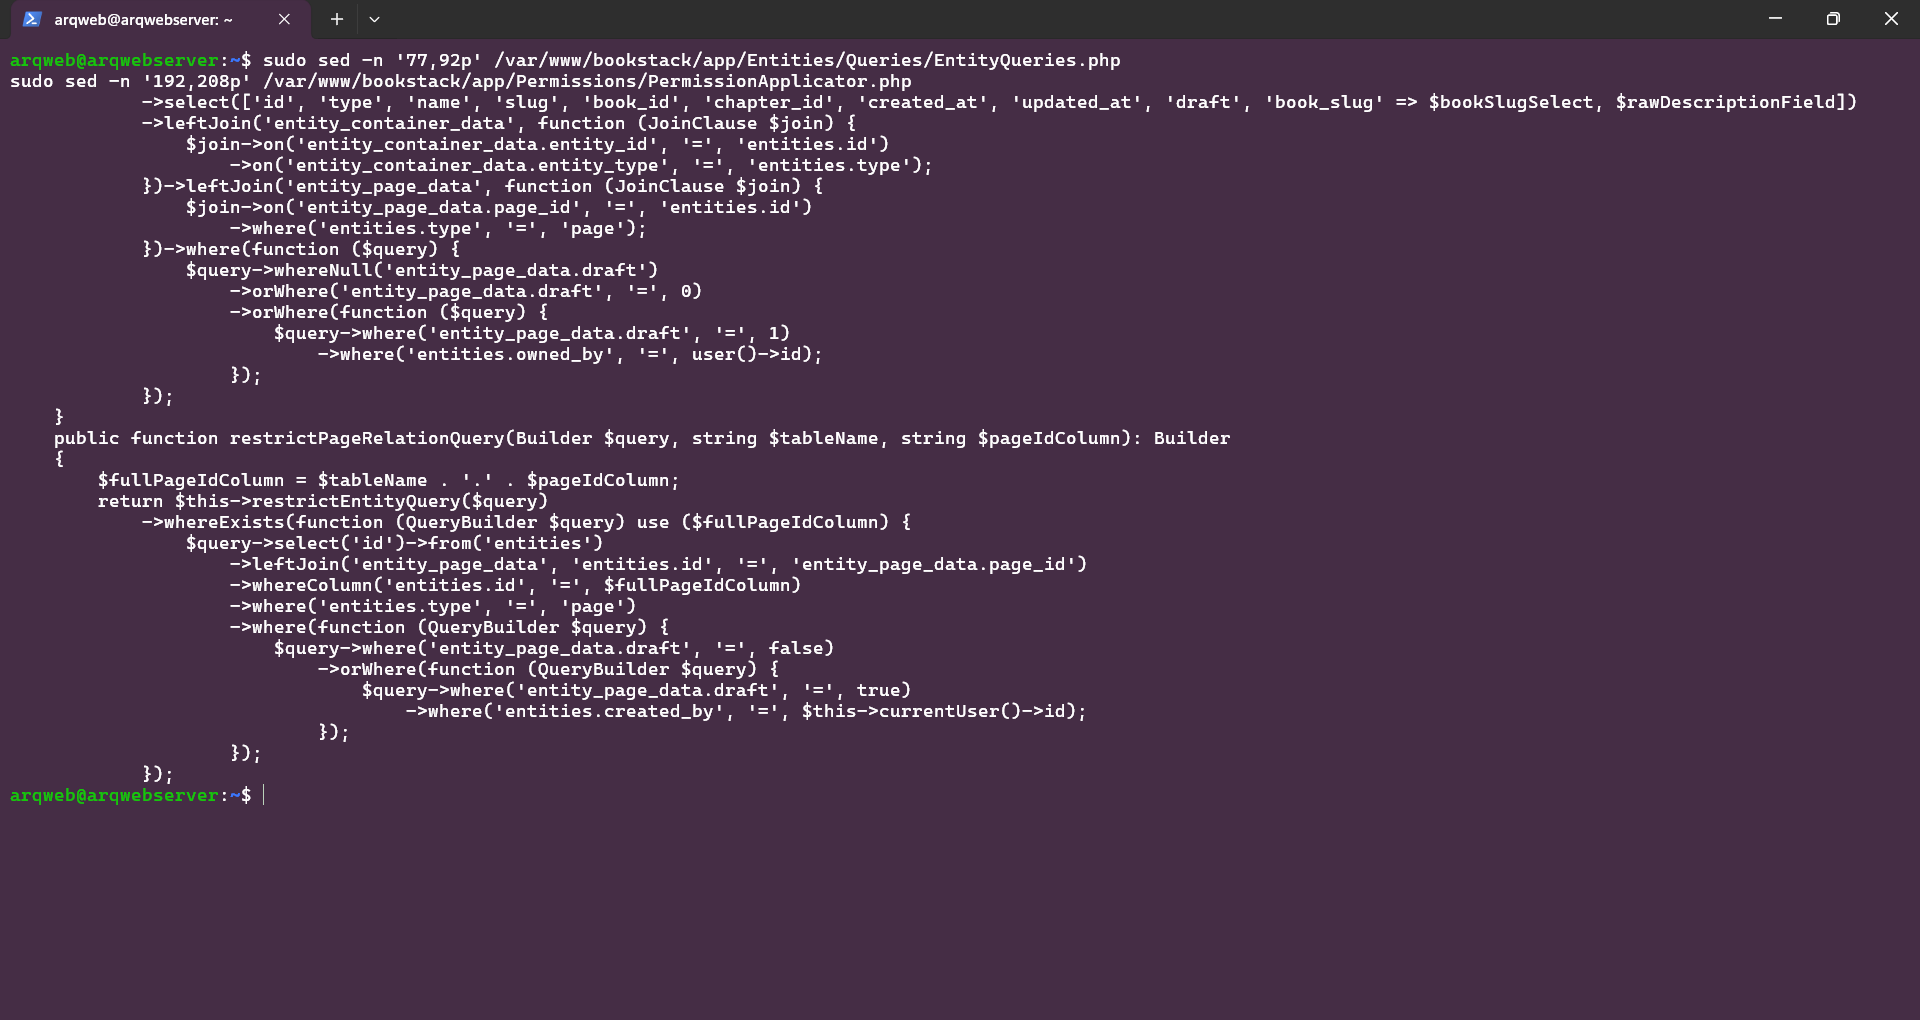
\includegraphics[width=\textwidth,height=0.64\textheight,keepaspectratio]{../../../cna/docs/evidencias/fase5/F5-E2-01-contenido-permisos.png}
\caption{Respaldo de F5-E2. Uniones compartidas de contenido y permisos, con filtros de borrador y propietario.}
\label{fig:f5-e2-contenido}
\end{figure}

\begin{figure}[H]
\centering
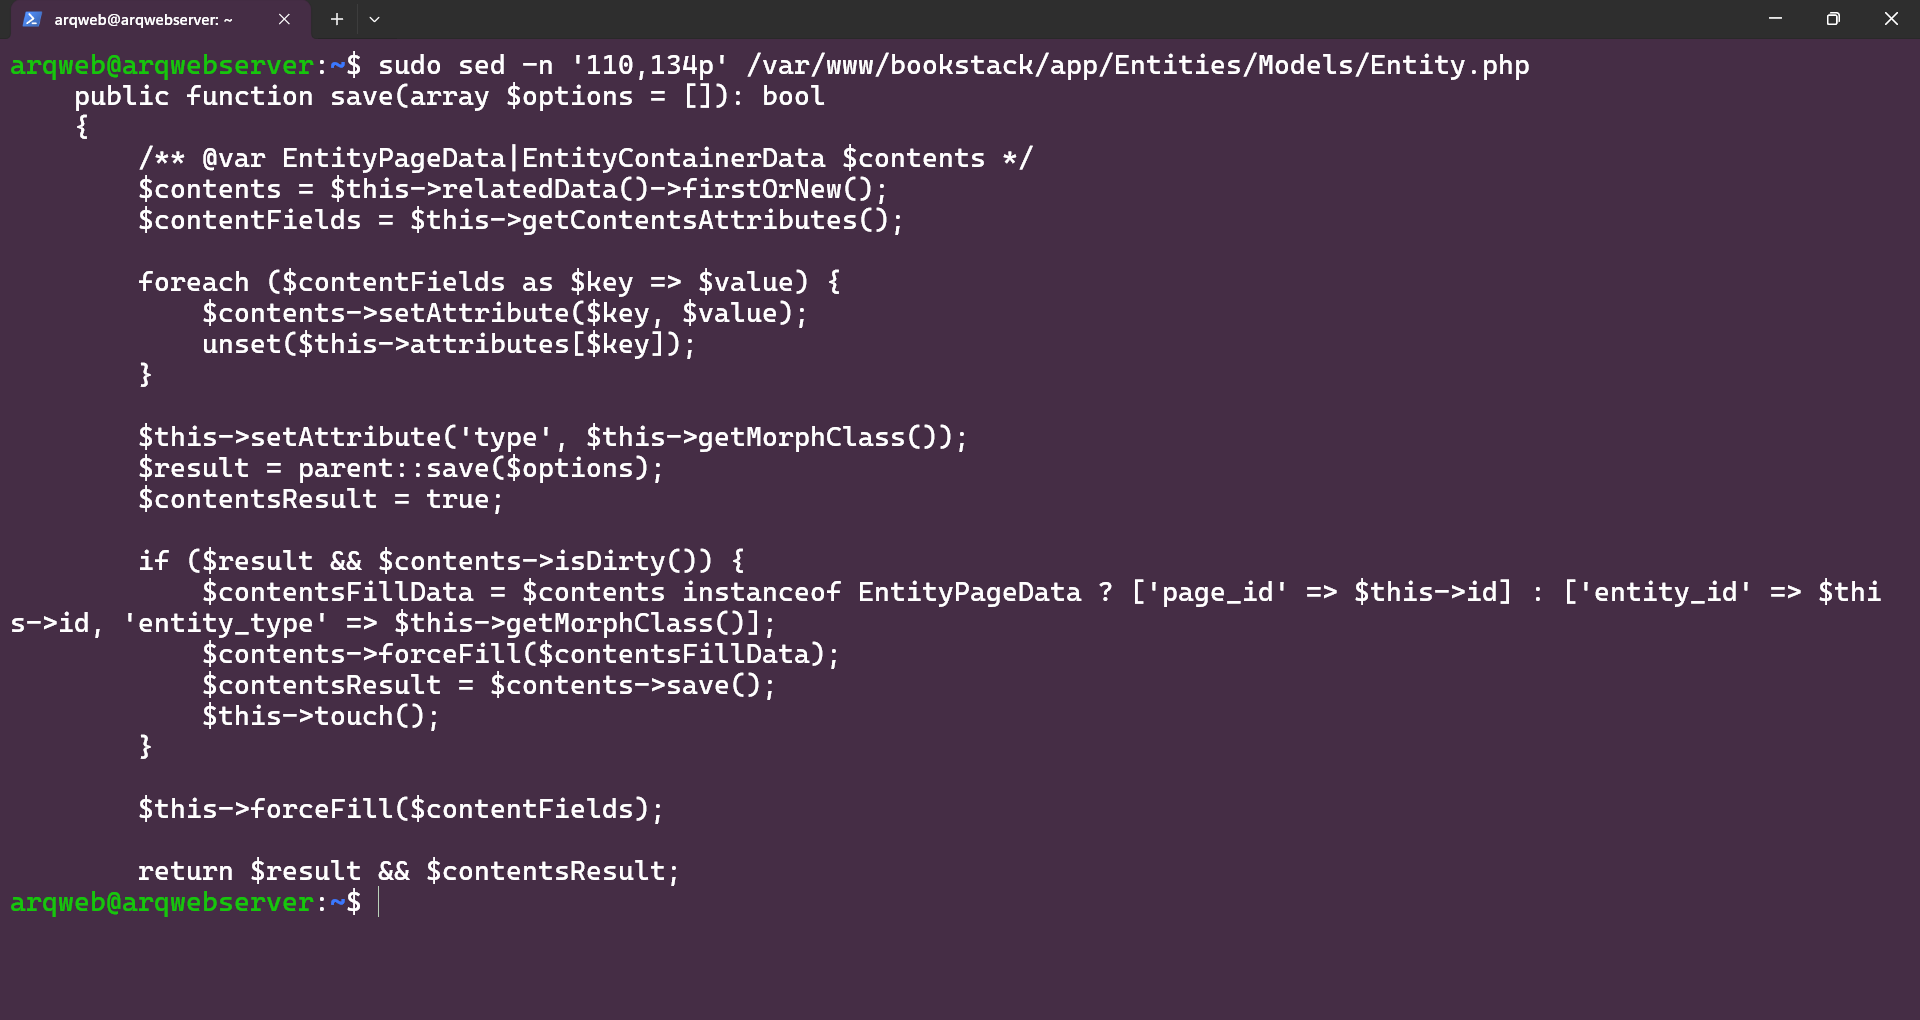
\includegraphics[width=\textwidth,height=0.64\textheight,keepaspectratio]{../../../cna/docs/evidencias/fase5/F5-E2-05-escritura-contenido.png}
\caption{Respaldo de F5-E2. Guardado de entidad y de sus datos específicos en el método Entity::save().}
\label{fig:f5-e2-escritura}
\end{figure}

\textbf{Búsqueda y actividad.} \texttt{SearchRunner} une los términos con
\texttt{entities} por ID y tipo. \texttt{SearchIndex} genera términos a partir
del nombre, el HTML o la descripción y las etiquetas, elimina el índice
previo e inserta los términos actualizados (R04).
\path{ActivityLogger::add()} guarda el registro de actividad antes de
llamar a \texttt{dispatchWebhooks()} (R05). Las
Figuras~\ref{fig:f5-e2-busqueda} y~\ref{fig:f5-e2-indice} respaldan las
consultas y escrituras identificadas.

\begin{figure}[H]
\centering
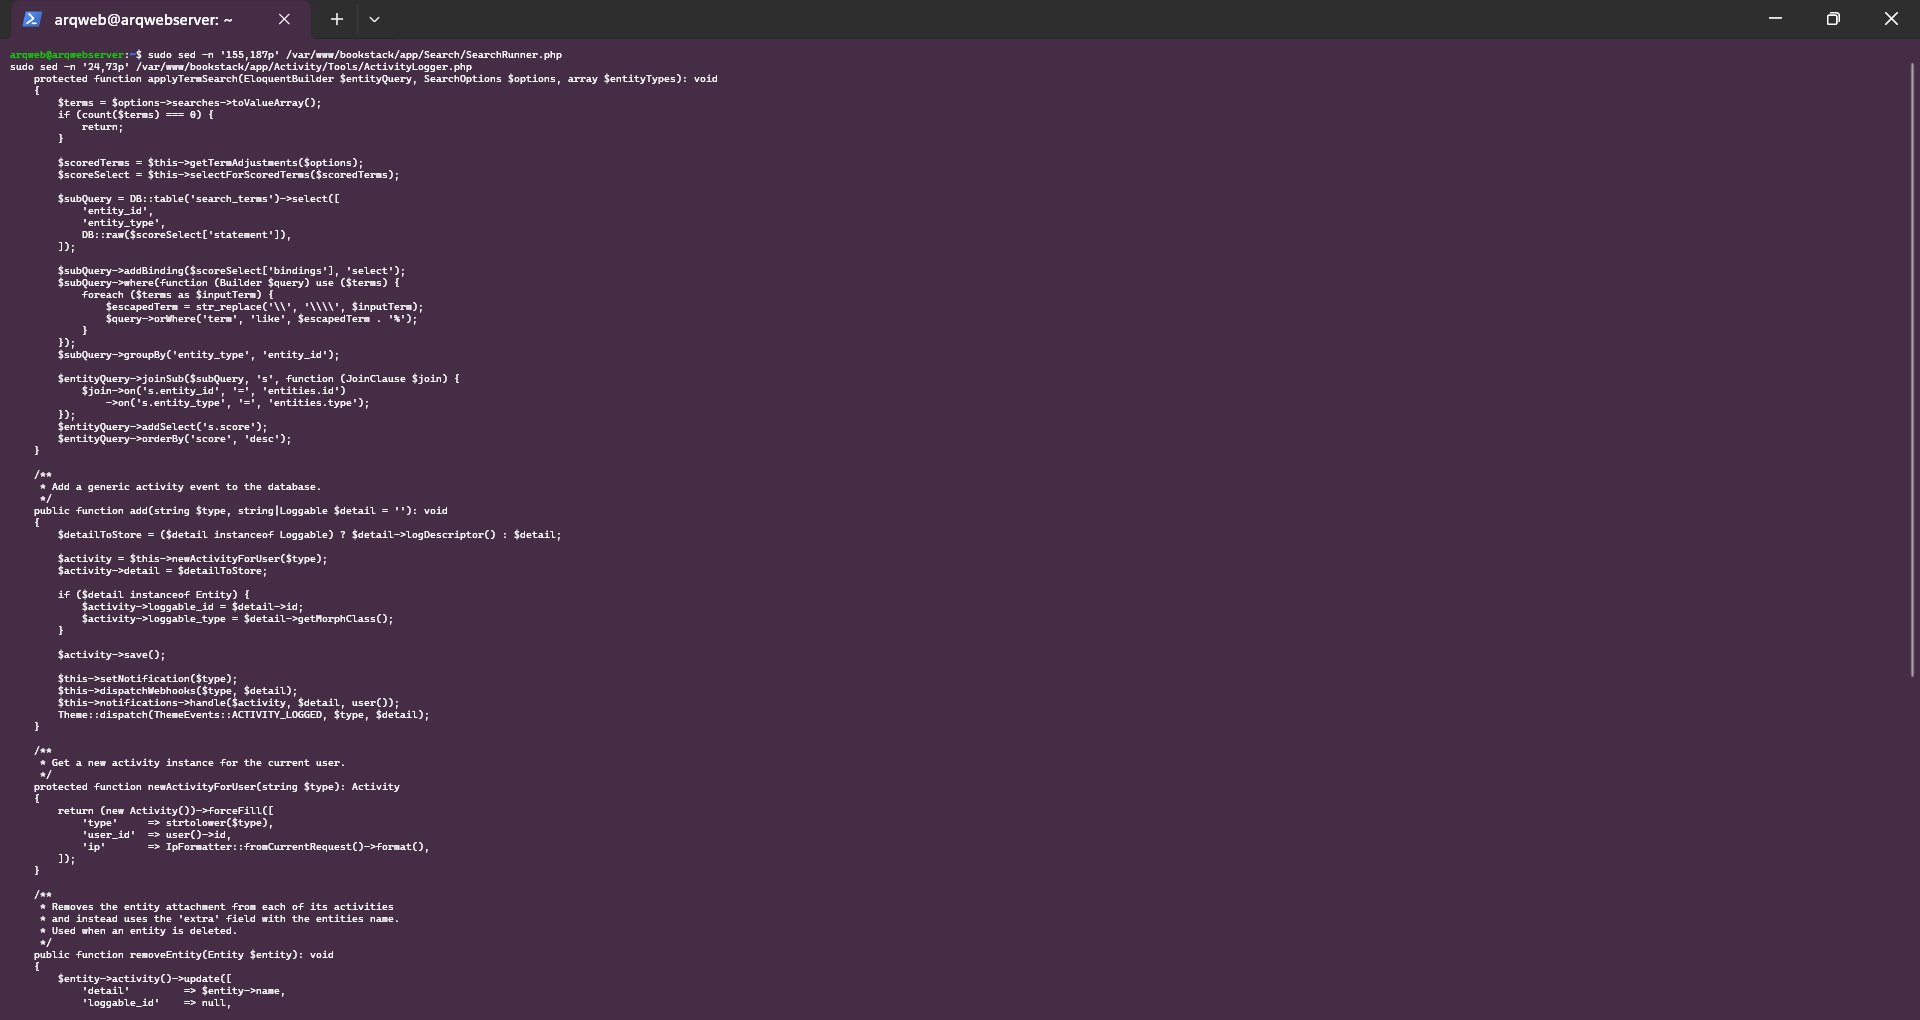
\includegraphics[width=\textwidth,height=0.64\textheight,keepaspectratio]{../../../cna/docs/evidencias/fase5/F5-E2-02-busqueda-auditoria.png}
\caption{Respaldo de F5-E2. Lectura del índice y persistencia de actividad con referencia al actor y al objeto.}
\label{fig:f5-e2-busqueda}
\end{figure}

\begin{figure}[H]
\centering
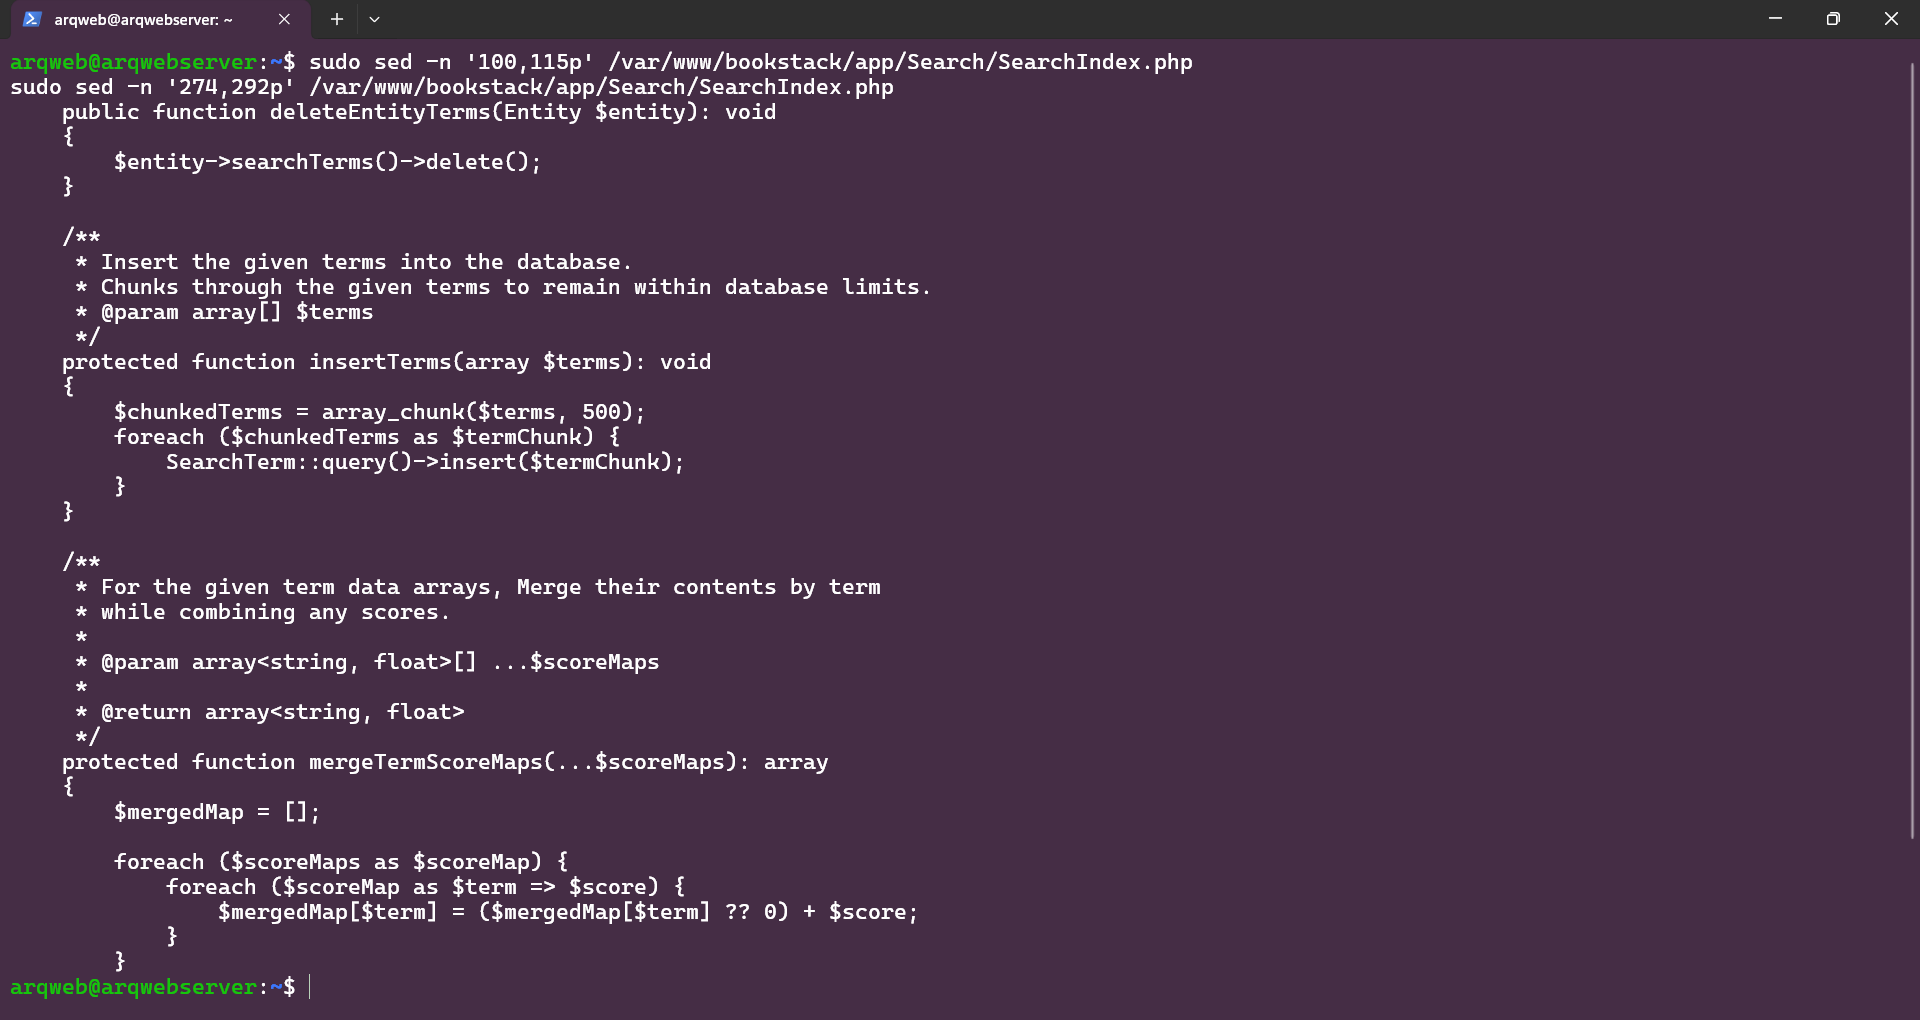
\includegraphics[width=\textwidth,height=0.64\textheight,keepaspectratio]{../../../cna/docs/evidencias/fase5/F5-E2-06-escritura-indice.png}
\caption{Respaldo de F5-E2. Eliminación de términos previos e inserción de los términos del índice de búsqueda.}
\label{fig:f5-e2-indice}
\end{figure}

\textbf{Imágenes y adjuntos.} \texttt{ImageService} guarda y elimina registros
y archivos; su limpieza de imágenes consulta el HTML de páginas y
revisiones para localizar referencias (R07,
Figura~\ref{fig:f5-e2-medios}). \texttt{AttachmentService} persiste los
metadatos de la subida, relaciona el archivo con la página por
\texttt{uploaded\_to} y coordina la baja del archivo y del registro
(R08, Figura~\ref{fig:f5-e2-adjuntos}). La visibilidad de los medios se
resuelve contra la página y sus permisos.

\begin{figure}[H]
\centering
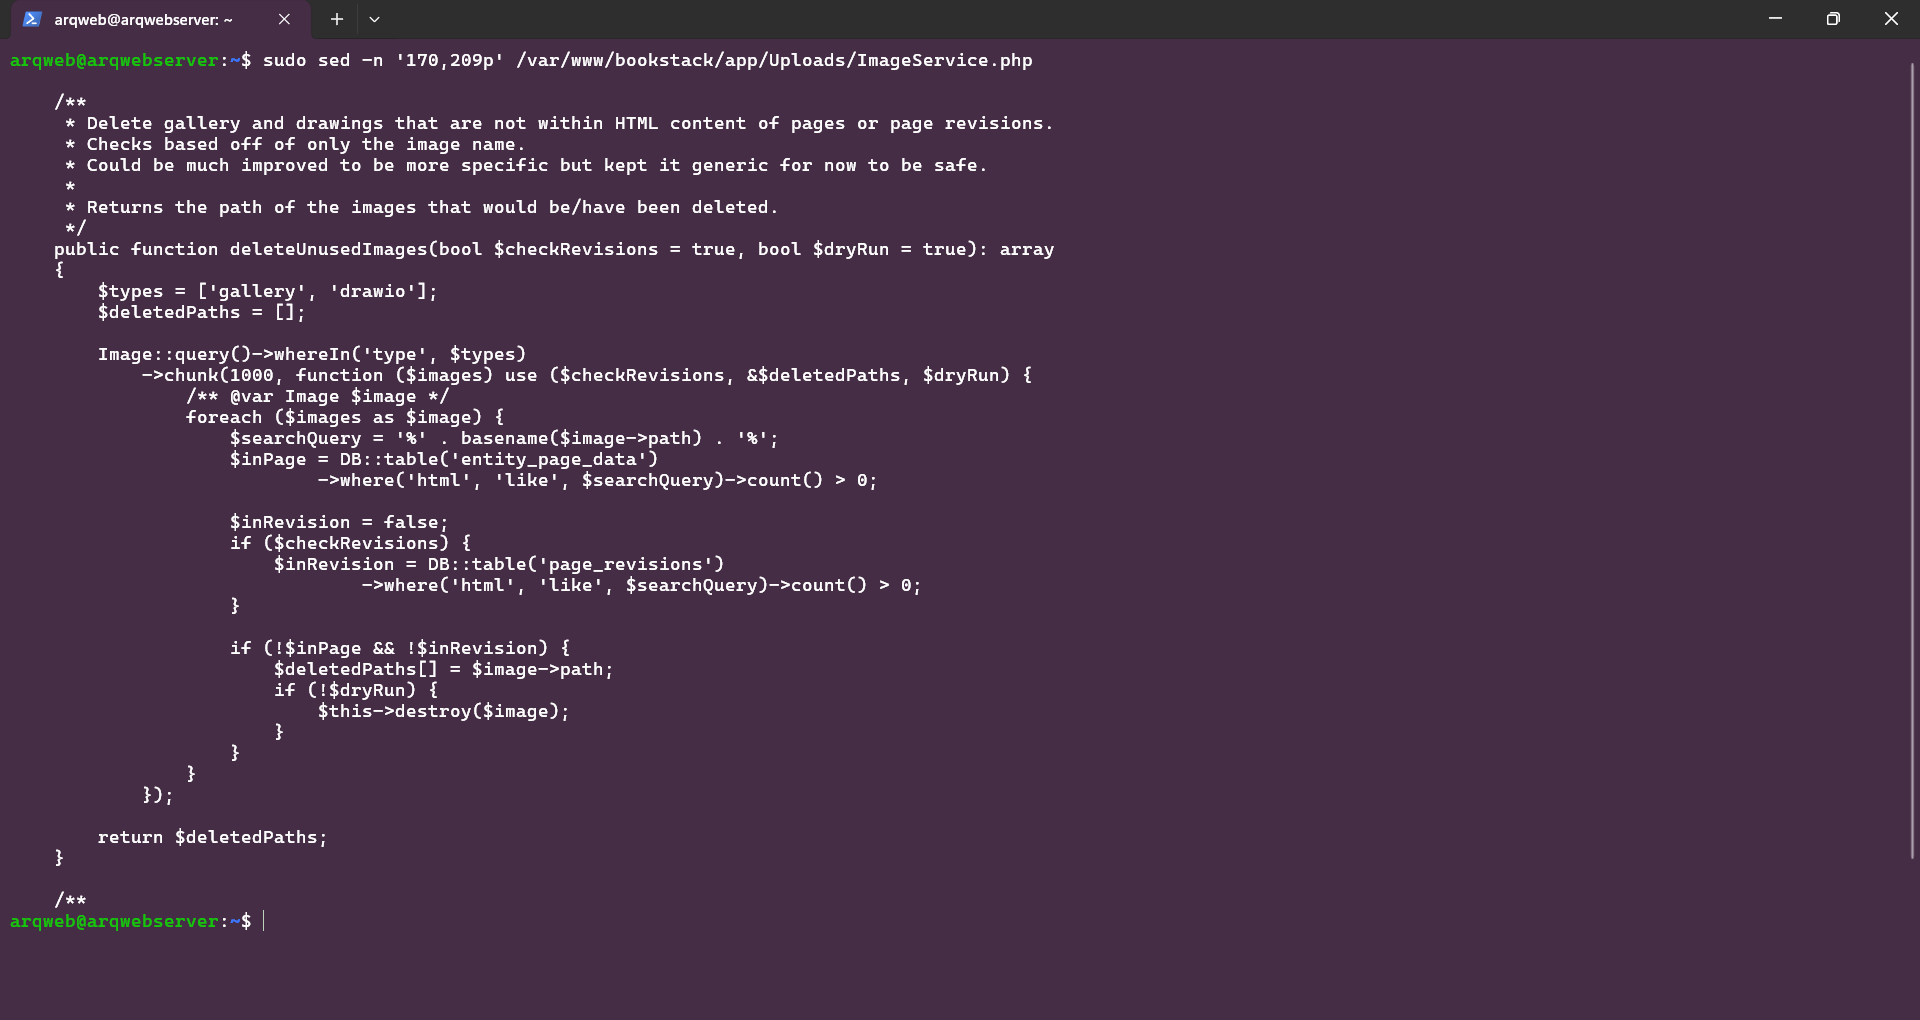
\includegraphics[width=\textwidth,height=0.64\textheight,keepaspectratio]{../../../cna/docs/evidencias/fase5/F5-E2-03-medios.png}
\caption{Respaldo de F5-E2. Dependencia de medios respecto del HTML actual e histórico para detectar imágenes sin uso.}
\label{fig:f5-e2-medios}
\end{figure}

\begin{figure}[H]
\centering
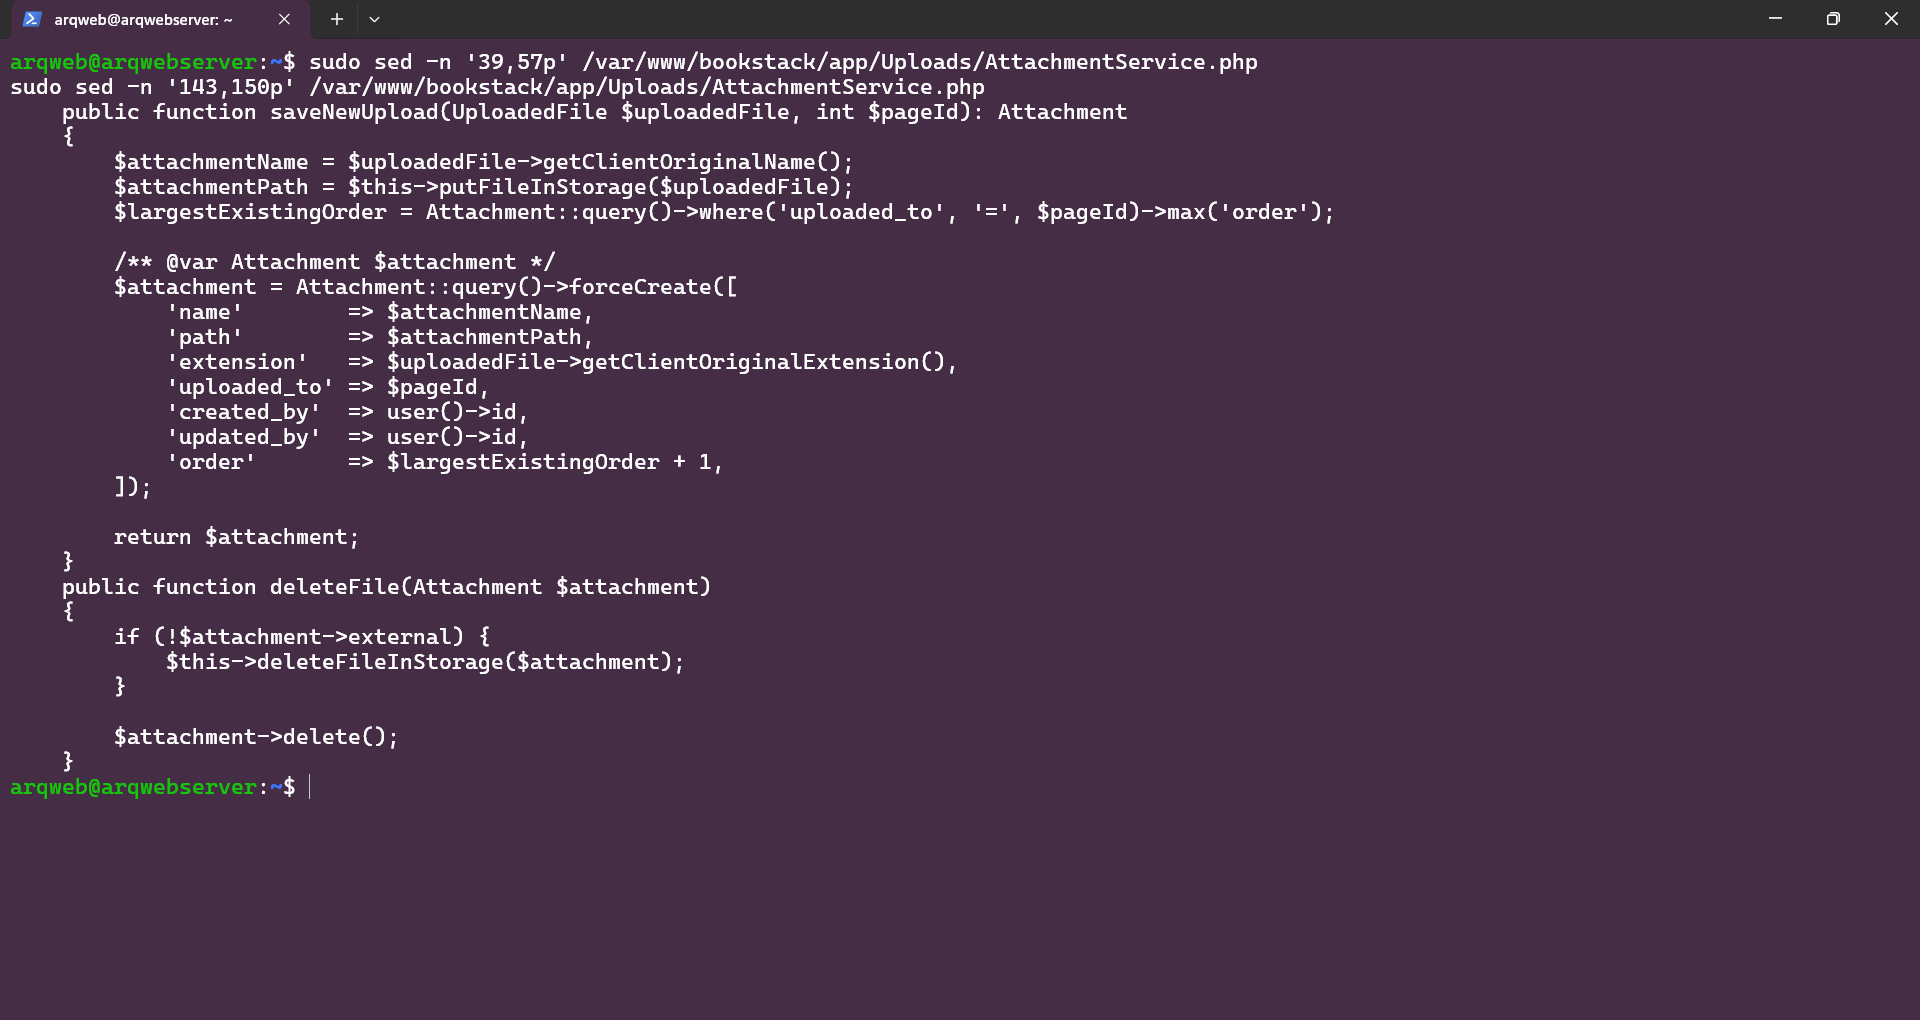
\includegraphics[width=\textwidth,height=0.64\textheight,keepaspectratio]{../../../cna/docs/evidencias/fase5/F5-E2-07-adjuntos.png}
\caption{Respaldo de F5-E2. Creación de metadatos de adjuntos y eliminación del archivo y su registro.}
\label{fig:f5-e2-adjuntos}
\end{figure}

\textbf{Usuarios, roles y permisos.} La consulta de permisos del usuario une
\texttt{role\_user}, \texttt{permission\_role} y \texttt{role\_permissions}.
\texttt{UserRepo} guarda cuentas y sincroniza roles
(Figura~\ref{fig:f5-e2-usuarios}). Al eliminar un usuario actualiza la autoría
en contenido, imágenes, adjuntos y revisiones, y reasigna la propiedad de
las entidades (Figura~\ref{fig:f5-e2-borrado}).
\texttt{PermissionsUpdater} modifica restricciones y
\path{JointPermissionBuilder} reconstruye \texttt{joint\_permissions}
(Figura~\ref{fig:f5-e2-permisos}). Estos recorridos explican el acceso
transversal a tablas administradas por otros módulos (R09--R10).

\begin{figure}[H]
\centering
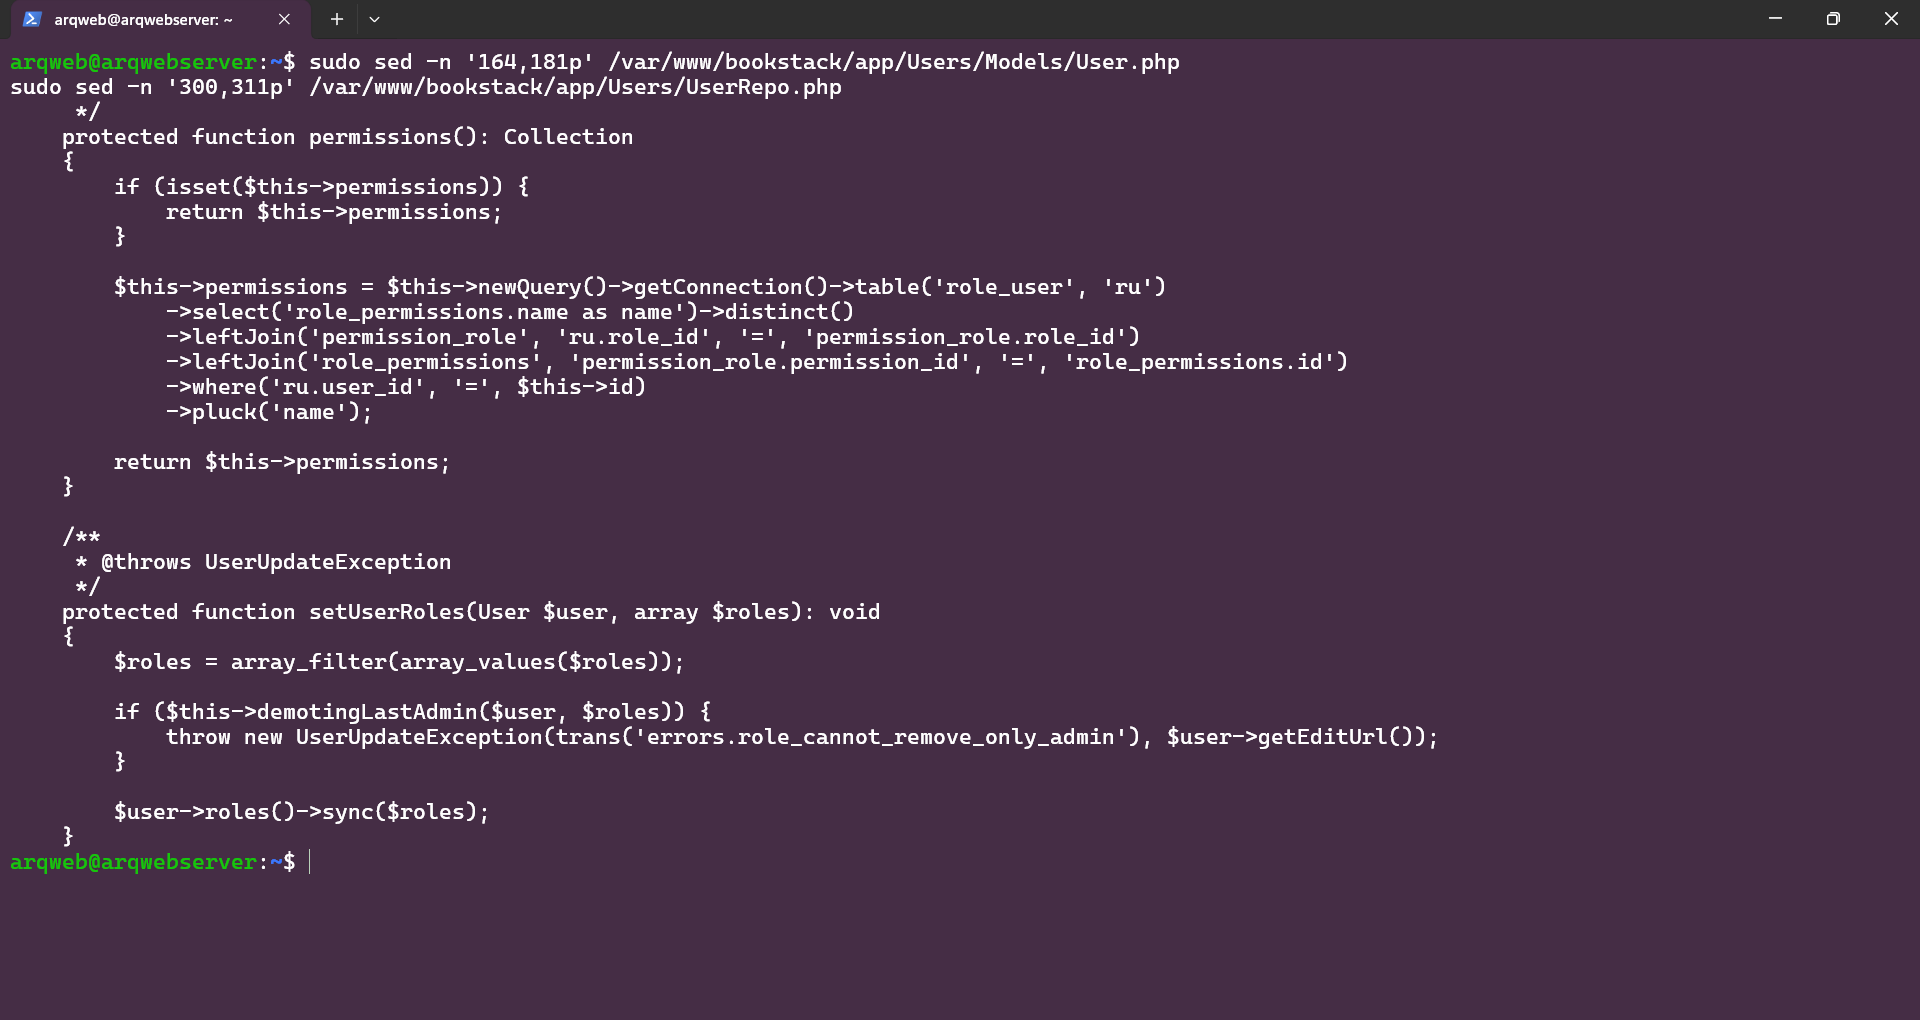
\includegraphics[width=\textwidth,height=0.64\textheight,keepaspectratio]{../../../cna/docs/evidencias/fase5/F5-E2-08-usuarios-roles.png}
\caption{Respaldo de F5-E2. Consulta de permisos del usuario y sincronización de su asignación de roles.}
\label{fig:f5-e2-usuarios}
\end{figure}

\begin{figure}[H]
\centering
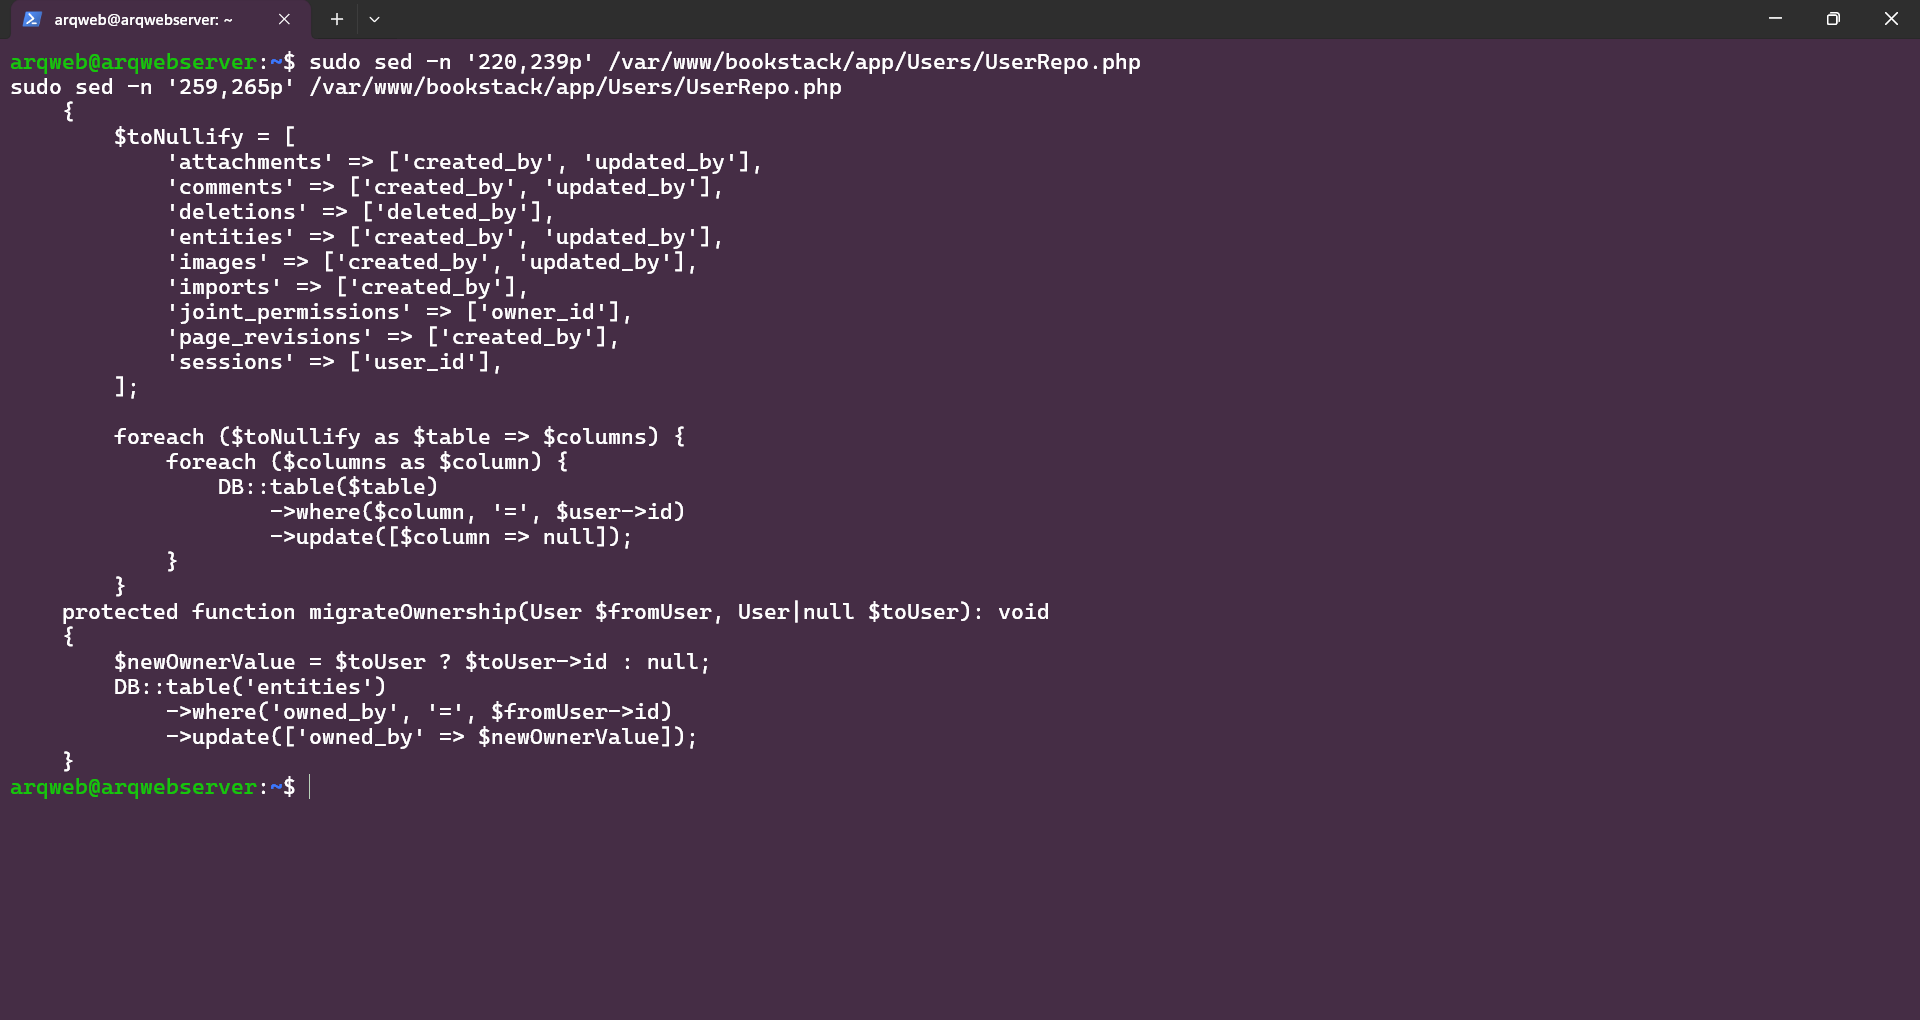
\includegraphics[width=\textwidth,height=0.64\textheight,keepaspectratio]{../../../cna/docs/evidencias/fase5/F5-E2-09-borrado-usuario.png}
\caption{Respaldo de F5-E2. Actualización de autoría y propiedad sobre tablas compartidas al eliminar una cuenta.}
\label{fig:f5-e2-borrado}
\end{figure}

\begin{figure}[H]
\centering
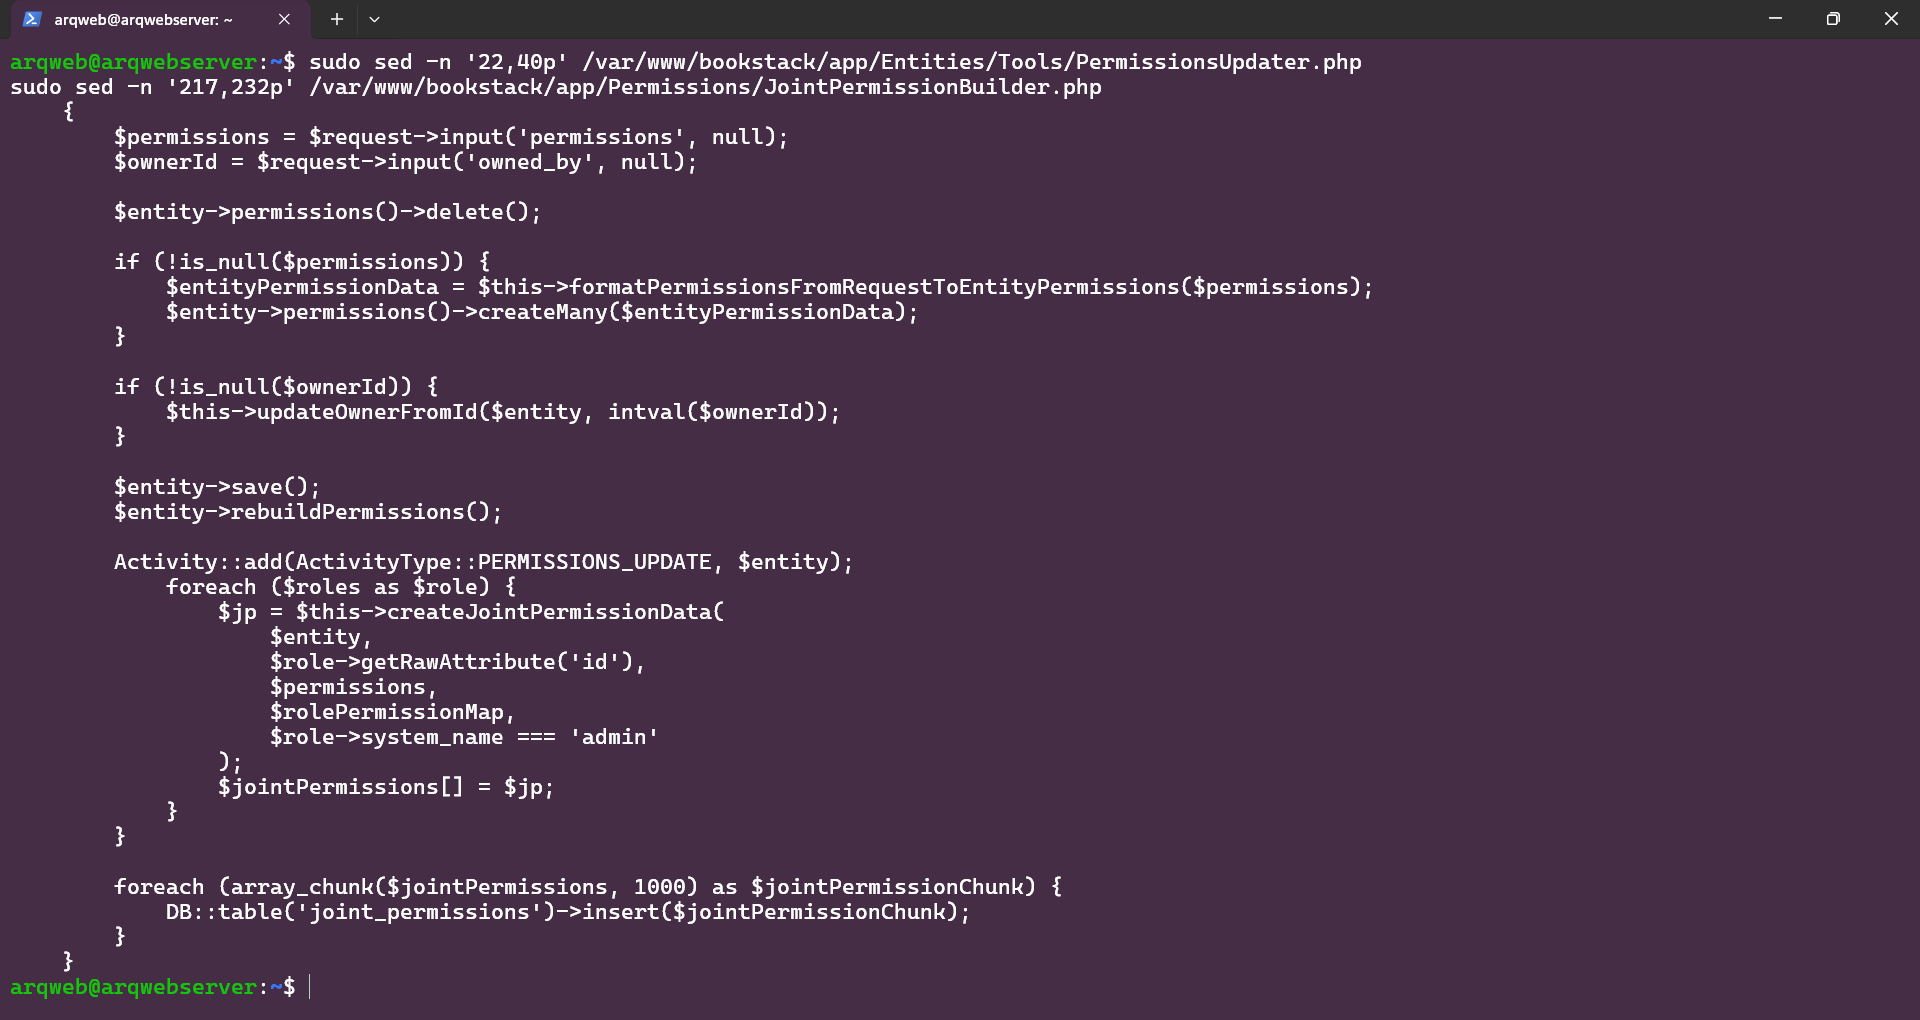
\includegraphics[width=\textwidth,height=0.64\textheight,keepaspectratio]{../../../cna/docs/evidencias/fase5/F5-E2-10-permisos-efectivos.png}
\caption{Respaldo de F5-E2. Persistencia de restricciones y reconstrucción de permisos efectivos.}
\label{fig:f5-e2-permisos}
\end{figure}

\textbf{Exportación.} Los controladores de API aplican el permiso
\texttt{ContentExport} y consultas visibles. El alcance de entidades une
los datos específicos; \texttt{BookContents} recupera el árbol de capítulos
y páginas. \texttt{ExportFormatter} obtiene Markdown o genera HTML para PDF
(R06, Figuras~\ref{fig:f5-e2-exporta} y~\ref{fig:f5-e2-exportb}). La ruta ZIP
lee etiquetas y adjuntos y recupera imágenes y archivos por sus modelos
(Figura~\ref{fig:f5-e2-zip}). La extracción debe conservar tanto la
visibilidad del contenido como el permiso de exportación.

\begin{figure}[H]
\centering
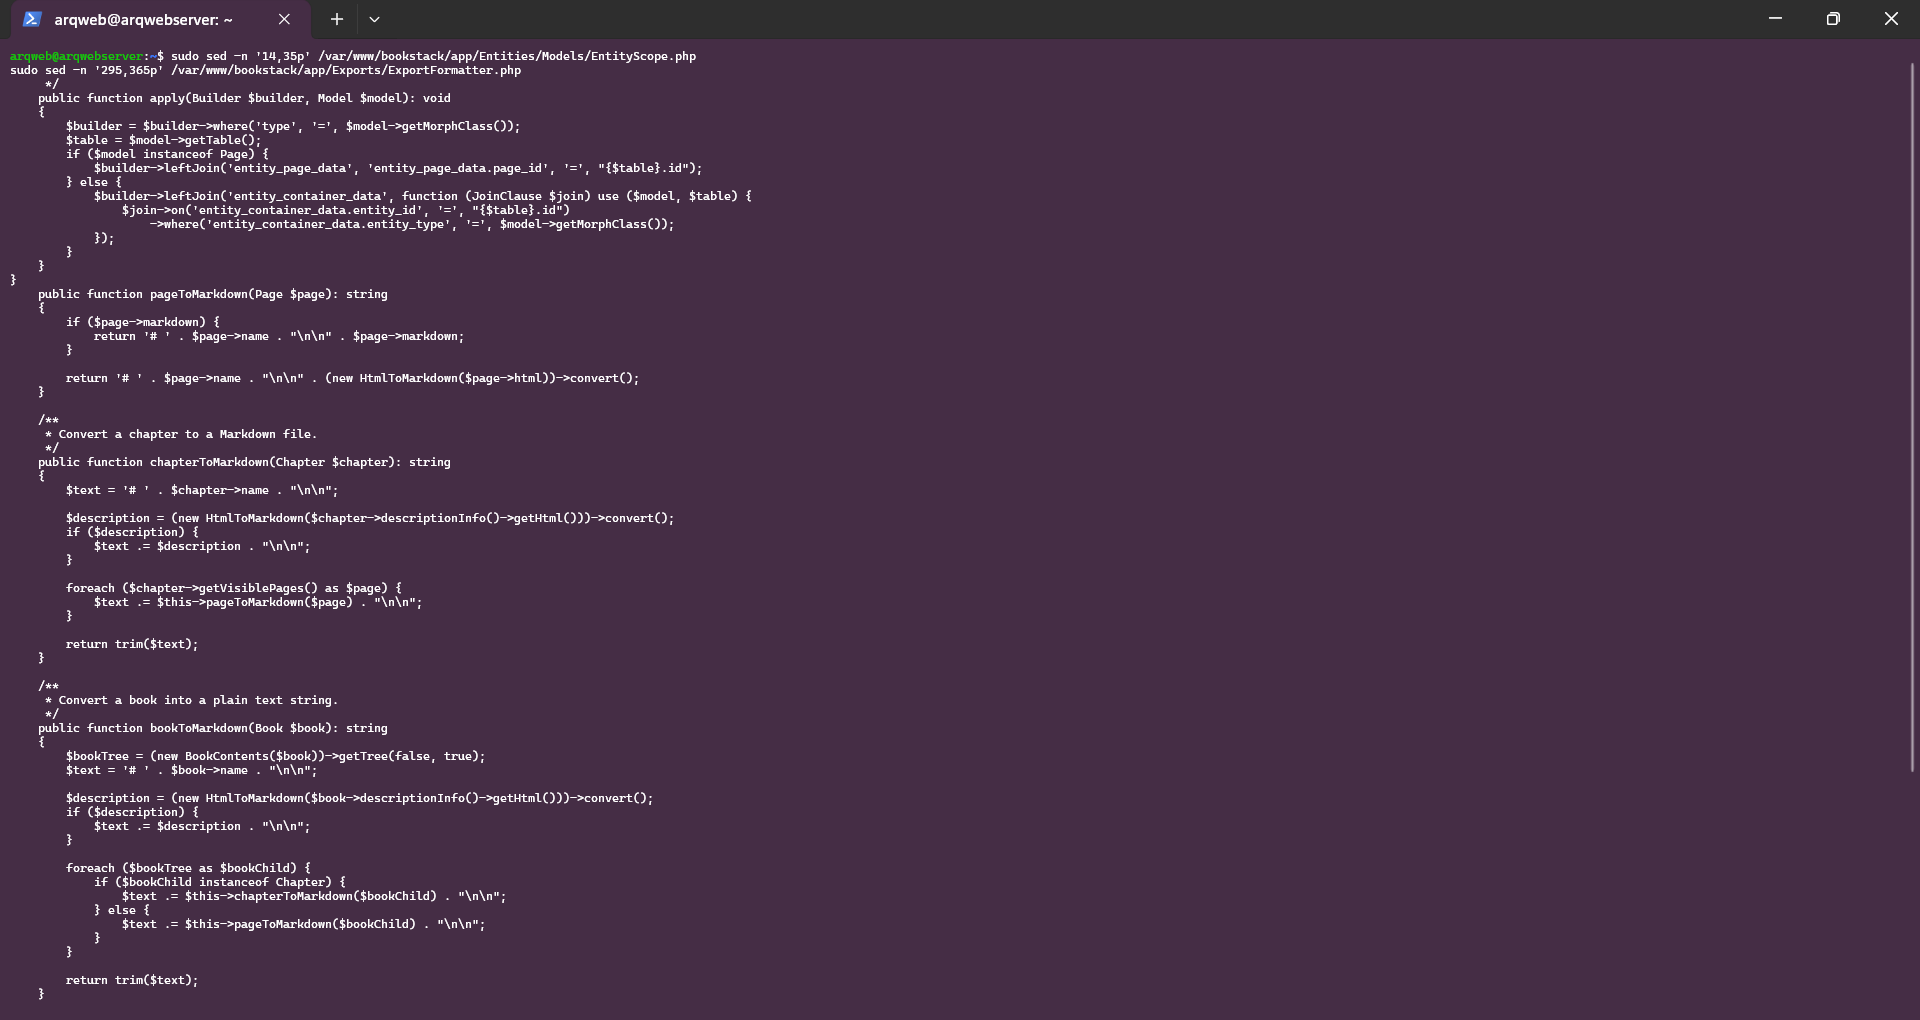
\includegraphics[width=\textwidth,height=0.64\textheight,keepaspectratio]{../../../cna/docs/evidencias/fase5/F5-E2-04-exportacion-markdown-a.png}
\caption{Respaldo de F5-E2. Alcance de entidades y conversión del contenido de página a Markdown.}
\label{fig:f5-e2-exporta}
\end{figure}

\begin{figure}[H]
\centering
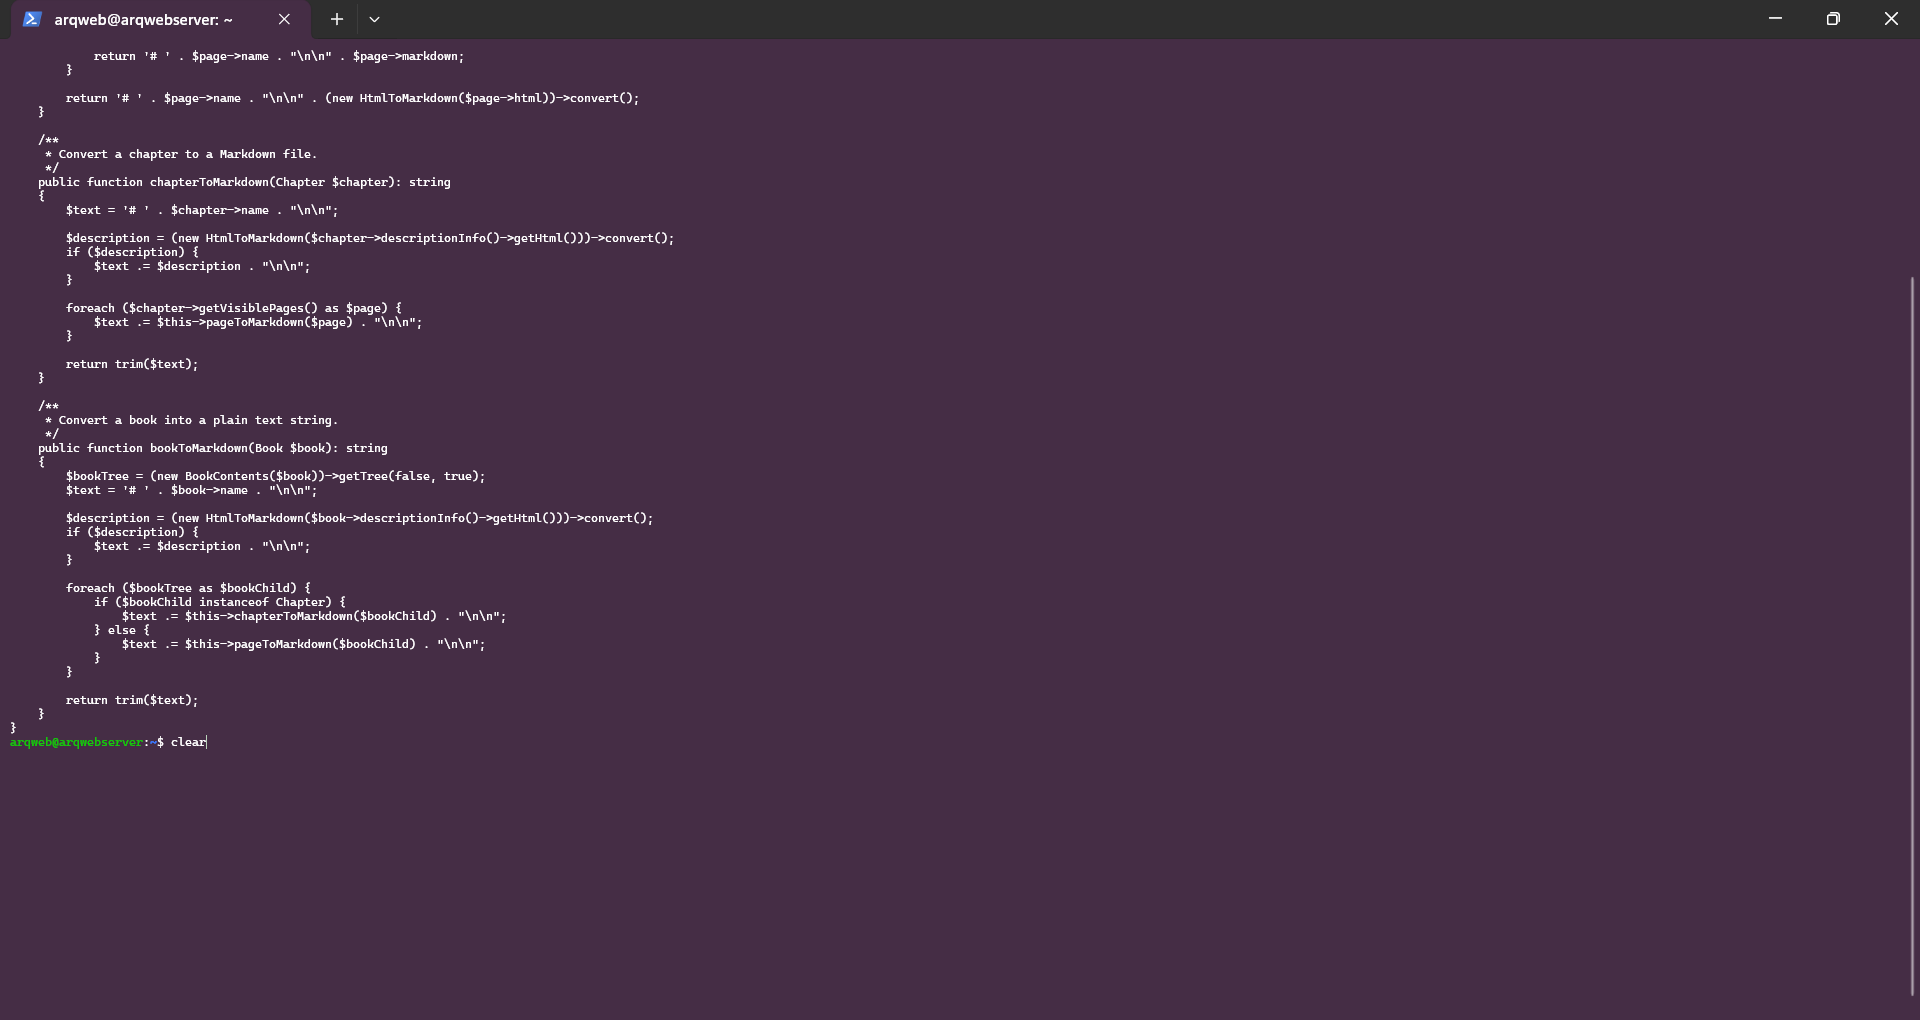
\includegraphics[width=\textwidth,height=0.64\textheight,keepaspectratio]{../../../cna/docs/evidencias/fase5/F5-E2-04-exportacion-markdown-b.png}
\caption{Respaldo de F5-E2. Recorrido de capítulos y páginas del libro durante la exportación Markdown.}
\label{fig:f5-e2-exportb}
\end{figure}

\begin{figure}[H]
\centering
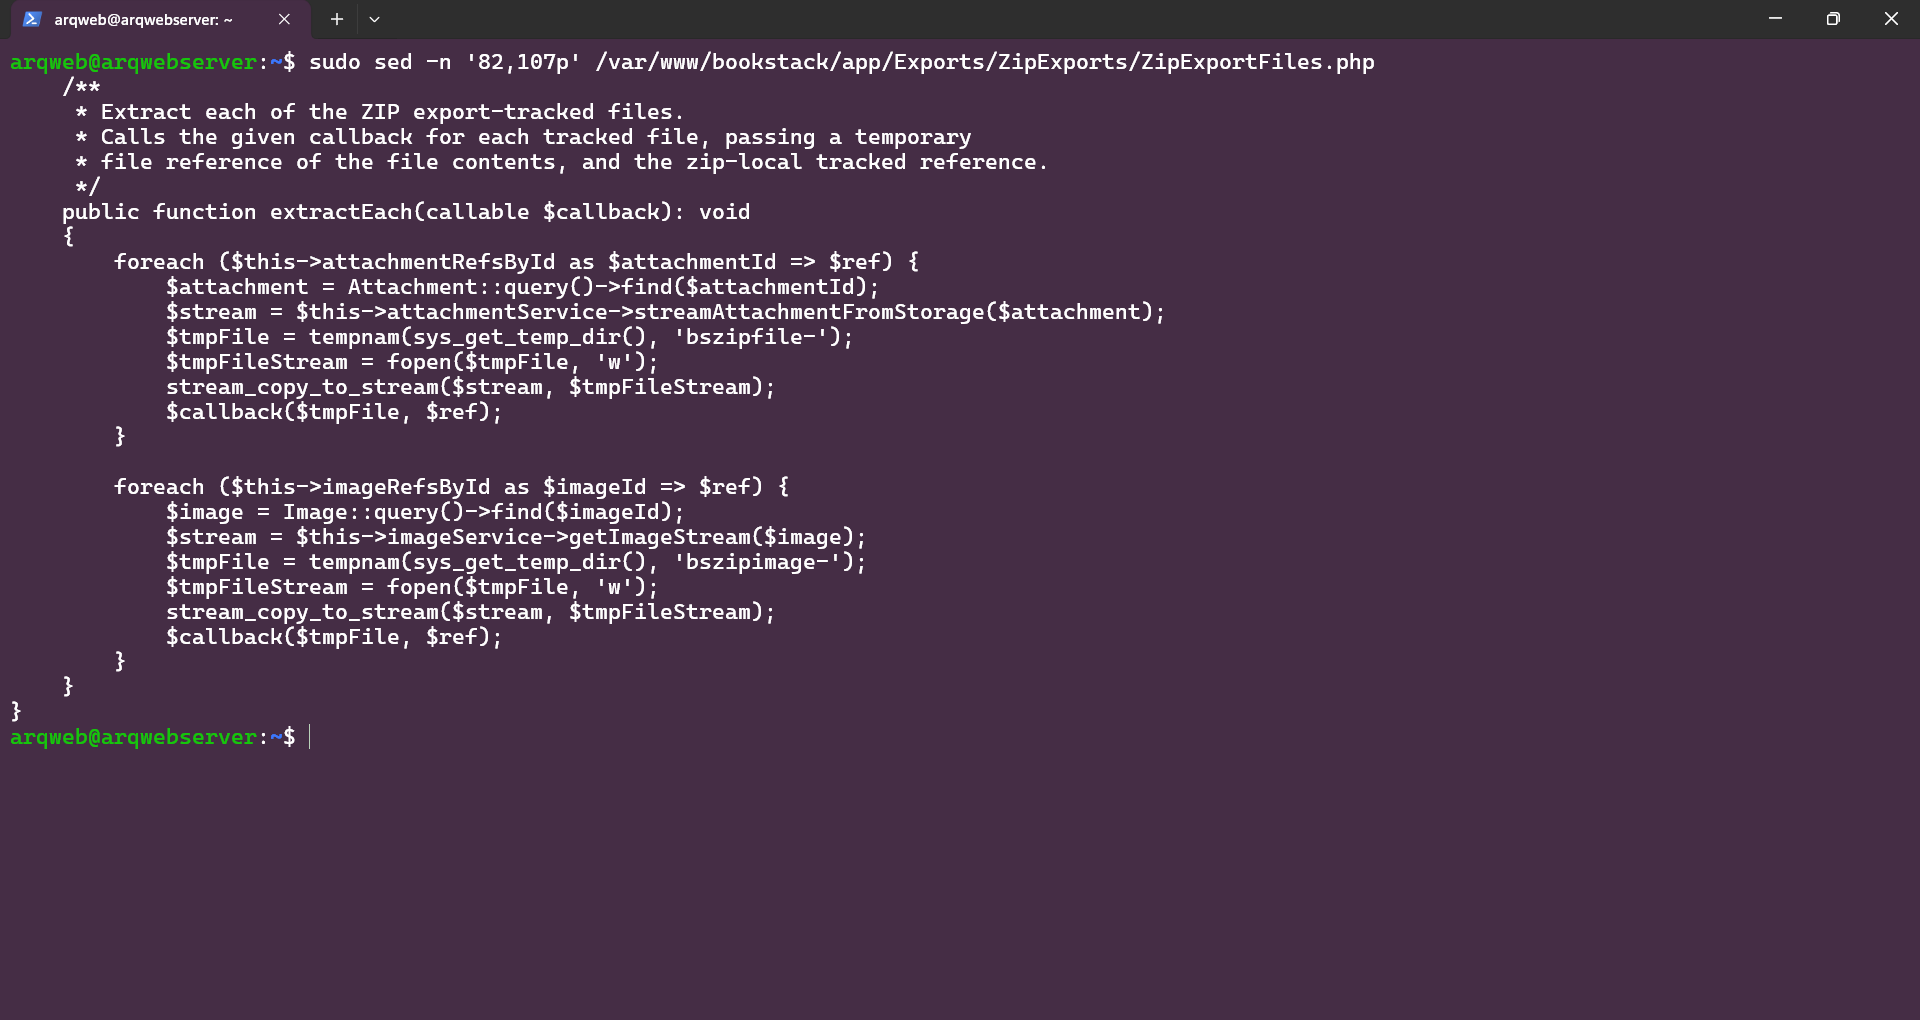
\includegraphics[width=\textwidth,height=0.64\textheight,keepaspectratio]{../../../cna/docs/evidencias/fase5/F5-E2-11-exportacion-archivos.png}
\caption{Respaldo de F5-E2. Lectura de adjuntos e imágenes para incorporar sus archivos a una exportación ZIP.}
\label{fig:f5-e2-zip}
\end{figure}

\subsubsection{Efecto de los acoplamientos sobre la extracción}
\begin{enumerate}[leftmargin=1.5em,itemsep=4pt]
\item \textbf{Contenido y búsqueda.} El guardado de contenido llama al indexador
local. La separación requiere un índice propio actualizado por eventos y
lecturas de API, con manejo de actualizaciones y borrados.
\item \textbf{Contenido y autorización.} La visibilidad depende de borradores,
propietario, roles y permisos efectivos. La consulta de datos mediante la
API y los resultados del nuevo servicio deben conservar ese alcance.
\item \textbf{Actividad y actores.} La auditoría registra acciones del contenido
y de la administración. La integración debe conservar actor, objeto, tipo
y momento de la acción mediante eventos normalizados.
\item \textbf{Medios y referencias.} La limpieza considera HTML y revisiones.
La gestión externa de archivos necesita preservar enlaces y referencias
para evitar eliminar recursos todavía utilizados.
\item \textbf{Exportación y contenido.} La exportación recorre entidades
visibles y puede incluir archivos. El servicio extraído consumirá la API
con autorización y administrará sus trabajos y artefactos propios.
\item \textbf{Usuarios y propiedad.} La eliminación de una cuenta actualiza
varias tablas. La representación de actores eliminados y la conservación
de sus referencias deben formar parte de los contratos de integración.
\end{enumerate}

\subsubsection{F5-E3: Mapa de contextos}
Se establecen seis contextos lógicos para analizar responsabilidades y
relaciones del dominio. La Figura~\ref{fig:f5-e3-contextos} representa su
situación actual dentro de BookStack. Las flechas indican información o
capacidad suministrada desde un proveedor hacia un consumidor. Los filtros
de autorización se aplican transversalmente en las consultas visibles.

\begin{figure}[H]
\centering
\begin{tikzpicture}[
ctx/.style={draw=NavyPrimary,fill=LightGrayBG,rounded corners=3pt,text width=3.5cm,minimum height=1.2cm,align=center,font=\small},
rel/.style={-{Stealth},thick,color=SlateSecondary},
lab/.style={font=\scriptsize,fill=white,inner sep=2pt,align=center}]
\node[ctx] (u) at (0,0) {Usuarios y permisos\\Proveedor de autorización};
\node[ctx] (c) at (0,-2.6) {Contenido\\Libros, capítulos y páginas};
\node[ctx] (m) at (-4.8,-2.6) {Imágenes y adjuntos\\Proveedor de archivos};
\node[ctx] (a) at (4.8,-2.6) {Actividad / auditoría\\Consumidor de acciones};
\node[ctx] (b) at (-2.5,-5.3) {Búsqueda\\Cliente de contenido};
\node[ctx] (x) at (2.5,-5.3) {Exportación\\Cliente de contenido};
\draw[rel] (u) -- node[lab,right]{Visibilidad y propiedad} (c);
\draw[rel] (m) -- node[lab,above]{Archivos} (c);
\draw[rel] (c) -- node[lab,above]{Acciones} (a);
\draw[rel] (c) -- node[lab,left]{Datos y etiquetas} (b);
\draw[rel] (c) -- node[lab,right]{Datos y árbol} (x);
\draw[rel] (u.east) -| node[lab,above,pos=0.3]{Acciones administrativas} (a.north);
\draw[rel] (c.north west) to[bend right=28] (m.north east);
\node[lab] at (-3.8,-1.1) {Referencias HTML\\y revisiones};
\end{tikzpicture}
\caption{F5-E3. Contextos lógicos del monolito y relaciones verificadas. Los seis contextos comparten el esquema de MariaDB; la matriz detalla sus accesos.}
\label{fig:f5-e3-contextos}
\end{figure}

\begin{samepage}
La relación de contenido con búsqueda y exportación se caracteriza como
\textit{cliente/proveedor}. Usuarios/permisos provee las reglas de acceso;
medios provee archivos y consulta referencias de contenido para su limpieza.
Actividad consume las acciones producidas por contenido y administración.
La persistencia compartida y las llamadas síncronas explican los límites
que deben adaptarse durante la extracción.
\end{samepage}

\begin{figure}[H]
\centering
\begin{tikzpicture}[
ctx/.style={draw=NavyPrimary,fill=LightGrayBG,rounded corners=3pt,text width=3.7cm,minimum height=1.1cm,align=center,font=\small},
acl/.style={ctx,draw=AccentBlue,fill=white},
rel/.style={-{Stealth},thick,color=SlateSecondary},
lab/.style={font=\scriptsize,fill=white,inner sep=2pt,align=center}]
\node[ctx,text width=7cm] (bs) at (0,0) {BookStack\\Contenido y autoridad de usuarios/permisos};
\node[acl] (http) at (-3.1,-2.2) {API REST\\Contenido autorizado};
\node[acl] (wh) at (3.1,-2.2) {Webhooks\\Acciones del monolito};
\node[acl] (ha) at (-3.1,-4.3) {ACL HTTP\\Adaptadores por servicio};
\node[acl] (ea) at (3.1,-4.3) {ACL de eventos\\event-bridge};
\node[ctx] (sx) at (-3.1,-6.6) {Búsqueda y exportación\\Clientes con datos propios};
\node[ctx] (ev) at (3.1,-6.6) {Canales de eventos\\Búsqueda y auditoría};
\draw[rel] (bs) -- (http);
\draw[rel] (bs) -- (wh);
\draw[rel] (http) -- (ha);
\draw[rel] (wh) -- (ea);
\draw[rel] (ha) -- node[lab,left]{Cliente/proveedor} (sx);
\draw[rel] (ea) -- node[lab,right]{Eventos normalizados} (ev);
\end{tikzpicture}
\caption{F5-E3. Límites de integración para la extracción. Las capas anticorrupción (ACL) adaptan la API y los Webhooks a contratos de los servicios consumidores.}
\label{fig:f5-e3-integracion}
\end{figure}

La ACL HTTP traduce las respuestas del monolito a las representaciones
propias de búsqueda y exportación. La ACL de eventos normaliza los Webhooks
antes de entregarlos a los consumidores. Medios constituye un contexto de
archivos y miniaturas con almacenamiento propio; su integración utiliza
URLs y API para conservar los recursos referenciados. El diseño de
contratos precisará el alcance de autorización y el ciclo de vida de los
archivos. La selección de herramientas y las decisiones de consistencia
se justifican en los ADR de A2.

Los fuentes editables del mapa se conservan en este archivo TikZ y en
\path{cna/docs/fase5-a1-contextos.mmd} y
\path{cna/docs/fase5-a1-contextos-propuesto.mmd}.

\subsubsection{Matriz de pruebas de A1 y resultado}
\begin{table}[H]
\centering\small
\begin{tabularx}{\textwidth}{p{1.3cm}p{1.8cm}Xp{2.3cm}}
\toprule
\textbf{Prueba} & \textbf{Evidencia} & \textbf{Resultado verificable} & \textbf{Estado} \\
\midrule
P26 & F5-E1 & Catálogo de 41 tablas y 280 columnas; cuatro FK; asignación de persistencia a los seis módulos. Tablas~\ref{tab:f5-modulos} y~\ref{tab:f5-fk}. & Completado \\
P27 & F5-E2 & Matriz de 6 módulos por 17 tablas principales, con accesos y dependencias delegadas respaldados por código. Tablas~\ref{tab:f5-matriz-1}--\ref{tab:f5-matriz-3}. & Completado \\
P28 & F5-E3 & Mapa de contextos, relaciones cliente/proveedor y capas anticorrupción. Figuras~\ref{fig:f5-e3-contextos} y~\ref{fig:f5-e3-integracion}. & Completado \\
\bottomrule
\end{tabularx}
\caption{Continuación de la matriz consolidada para A1, desde P26.}
\label{tab:f5-pruebas}
\end{table}

A1 establece el inventario de los seis módulos, su acoplamiento sobre tablas
compartidas y los límites de contexto para la extracción. La matriz vincula
las lecturas y escrituras con el código instalado y el mapa define las
relaciones funcionales y de integración que servirán de base a los ADR.


\endgroup

% !TeX root = main.tex
\clearpage
\begingroup
\setlength{\emergencystretch}{3em}
\subsection{A2: Registro de Decisiones de Arquitectura}
\label{sec:fase5-a2}
Se documentan las decisiones ADR-006 a ADR-010 aceptadas por el equipo para el diseño. Cada registro conserva contexto, decisión, alternativas descartadas y consecuencias. Las verificaciones operativas se ejecutarán durante la Fase 6. El respaldo de recursos del anfitrión se conserva en \path{cna/docs/adr/recursos-a2.txt}.

\subsubsection{ADR-006 — Estrategia de migración e integración con el monolito}
\label{adr:006}

\begin{adrbox}{Estatus de ADR-006}
Aceptado para el diseño por el equipo.
\end{adrbox}

\par\medskip\noindent\textbf{Contexto}\par\nobreak\smallskip

BookStack debe continuar atendiendo la gestión documental durante la extracción de búsqueda, auditoría, exportación y medios. La consigna establece integración por API REST y Webhooks y exige conservar el código fuente del monolito.

En A1 se verificó que el guardado de entidades persiste atributos comunes y específicos, invoca la indexación y registra actividad. La visibilidad de contenido y archivos depende de usuarios y permisos efectivos. Estos acoplamientos hacen necesario definir una frontera de integración que mantenga la autorización y permita incorporar los servicios gradualmente.

\par\medskip\noindent\textbf{Decisión}\par\nobreak\smallskip

Aplicar Strangler Fig incorporando los servicios alrededor de BookStack. El Nginx de VM-1 expondrá las rutas \path{/v2/} de los servicios mediante el dominio \path{api.bookstack.local}. BookStack mantendrá la gestión documental y su dominio actual.

Los servicios que necesitan contenido lo obtendrán mediante la API REST, con una cuenta de servicio y los permisos necesarios para cada operación. Los cambios de páginas se recibirán por Webhooks en \path{event-bridge}, que adaptará los mensajes a los contratos de eventos y los publicará para sus consumidores. Cada adaptador HTTP o de eventos funcionará como capa anticorrupción entre los modelos del monolito y los contratos de los servicios.

La habilitación de las nuevas funcionalidades será gradual. El gateway permitirá desactivar una ruta del servicio y devolver el acceso a la funcionalidad equivalente del monolito conforme al procedimiento de reversión que se documentará en A5.

\par\medskip\noindent\textbf{Alternativas descartadas}\par\nobreak\smallskip

\begin{itemize}[leftmargin=1.5em,itemsep=3pt]
\item \textbf{Reemplazar BookStack en una sola entrega.} Concentra el riesgo de migración de contenido, usuarios y permisos en una única intervención y dificulta conservar la operación durante la transición.
\item \textbf{Integrar los servicios mediante consultas directas a MariaDB.} Acopla los servicios a las tablas compartidas observadas en A1 y puede omitir los filtros de autorización de BookStack. Además, incumple la restricción docente de acceso a MariaDB desde los microservicios.
\item \textbf{Modificar BookStack para invocar los nuevos servicios.} Obliga a mantener cambios propios sobre el código del monolito y contradice la vía de integración exigida por la consigna.
\end{itemize}

\par\medskip\noindent\textbf{Consecuencias}\par\nobreak\smallskip

\par\medskip\noindent\textbf{Favorables}\par\nobreak\smallskip

\begin{itemize}[leftmargin=1.5em,itemsep=3pt]
\item Permite incorporar y verificar una funcionalidad por vez manteniendo la gestión documental disponible.
\item Usa las interfaces del monolito como frontera de integración y conserva sus controles de acceso en las lecturas de API.
\item Facilita desactivar una ruta externa ante fallos del servicio extraído.
\item Los contratos propios permiten evolucionar los servicios con persistencia independiente.
\end{itemize}

\par\medskip\noindent\textbf{Costos y limitaciones}\par\nobreak\smallskip

\begin{itemize}[leftmargin=1.5em,itemsep=3pt]
\item La API de BookStack pasa a ser una dependencia de los servicios de búsqueda y exportación, con latencia adicional y necesidad de timeouts y tratamiento de errores.
\item El índice y la auditoría externa se actualizarán de forma asíncrona, por lo que habrá un intervalo de consistencia eventual.
\item La integración necesita operación adicional de gateway, adaptadores, broker y credenciales, además de observabilidad entre componentes.
\item La lectura con un token de servicio exige definir el alcance de visibilidad de los resultados del servicio, especialmente en búsqueda y exportación.
\item La recolección inicial y la recuperación ante eventos fallidos requieren procedimientos explícitos. Su entrega, deduplicación y reintento se especificarán en ADR-007 y ADR-010.
\end{itemize}

\par\medskip\noindent\textbf{Respaldo y validación prevista}\par\nobreak\smallskip

El inventario, la matriz y los mapas de A1 respaldan el contexto de esta decisión. En Fase 6 se verificará la lectura mediante API, el recorrido edición \ensuremath{\rightarrow} Webhook \ensuremath{\rightarrow} evento \ensuremath{\rightarrow} reindexación y el acceso mediante gateway. La implementación se contrastará con esos resultados antes de considerar validado el diseño.

\clearpage
\subsubsection{ADR-007 — Selección del broker de mensajes}
\label{adr:007}

\begin{adrbox}{Estatus de ADR-007}
Aceptado para el diseño por el equipo. Validación operativa prevista en Fase 6.
\end{adrbox}

\par\medskip\noindent\textbf{Contexto}\par\nobreak\smallskip

Una edición de BookStack debe actualizar búsqueda y auditoría mediante el mismo evento. Los consumidores necesitan posiciones independientes y recuperación de mensajes publicados mientras están detenidos. Se requieren persistencia, confirmación manual, reintentos limitados y mensajes fallidos conservados para diagnóstico. El laboratorio tiene recursos de memoria acotados.

\par\medskip\noindent\textbf{Decisión}\par\nobreak\smallskip

Usar NATS con JetStream habilitado como broker de eventos. Configurar un stream de páginas con almacenamiento en archivo sobre un volumen persistente y consumidores pull durables independientes para búsqueda y auditoría. Cada consumidor tendrá confirmación explícita después de persistir su resultado. Los trabajos de exportación conservarán su mecanismo de cola propio conforme a ADR-009.

El refinamiento del contrato A3 establece que \path{event-bridge} guardará inbox y outbox de forma atómica antes de devolver 202 al Webhook. El publicador esperará la confirmación de JetStream antes de marcar la salida como enviada. Mantendrá el mismo \path{event_id} al reintentar el evento normalizado y deduplicará la entrada conforme al contrato del puente.

El diseño inicial utiliza un broker con una réplica de almacenamiento. Esto cubre reinicios del proceso y del nodo con el mismo disco disponible. La réplica única concentra la disponibilidad del broker en ese nodo y no protege frente a pérdida del volumen.

Se usarán límites explícitos de memoria, disco y retención. La capacidad y el período de conservación deben cubrir las pruebas de caída de consumidores y medirse antes del despliegue final. La recuperación a DLQ se implementará explícitamente conforme a ADR-010. Alcanzar \path{MaxDeliver} en JetStream no equivale a mover automáticamente el mensaje a una DLQ.

\par\medskip\noindent\textbf{Alternativas descartadas}\par\nobreak\smallskip

\begin{table}[H]
\centering\small
\begin{tabularx}{\textwidth}{>{\raggedright\arraybackslash}X>{\raggedright\arraybackslash}X>{\raggedright\arraybackslash}X}
\toprule
\textbf{Alternativa} & \textbf{Qué ofrece} & \textbf{Motivo de descarte para este diseño} \\
\midrule
RabbitMQ & Acknowledgements, publisher confirms, enrutamiento y dead-lettering configurable. & Es válido para el TP, pero requeriría adoptar su modelo de exchanges, colas y políticas. Se prefiere el modelo de stream con consumidores independientes para los eventos de páginas. El consumo relativo de RAM entre productos no se considera medido. \\
Redis Streams como broker general & Streams, grupos de consumidores, pendientes y recuperación de trabajo. & Redis se reserva para los trabajos de exportación. Separar el broker de eventos permite administrar su retención y consumidores sin compartir el ciclo de vida de los jobs. Redis Streams también necesitaría políticas explícitas de persistencia y mensajes fallidos. \\
Core NATS sin JetStream & Pub/sub entre procesos conectados. & La persistencia y recuperación de eventos durante la caída de consumidores requieren JetStream. \\
\bottomrule
\end{tabularx}
\caption{Comparación y alcance de la decisión ADR-007.}
\label{tab:adr-007}
\end{table}

\par\medskip\noindent\textbf{Consecuencias}\par\nobreak\smallskip

\par\medskip\noindent\textbf{Favorables}\par\nobreak\smallskip

\begin{itemize}[leftmargin=1.5em,itemsep=3pt]
\item Un mismo evento de página puede ser procesado por búsqueda y auditoría con cursores separados.
\item El consumidor puede recuperar mensajes pendientes después de un reinicio.
\item Los ack explícitos permiten confirmar después de guardar el efecto del evento.
\item Stream y consumidores forman una frontera de integración independiente de las tablas de BookStack.
\end{itemize}

\par\medskip\noindent\textbf{Costos y limitaciones}\par\nobreak\smallskip

\begin{itemize}[leftmargin=1.5em,itemsep=3pt]
\item Hay que operar el volumen, los límites de retención, el monitoreo de pendientes y el procedimiento de DLQ.
\item La entrega al menos una vez permite duplicados, por lo que exige idempotencia en cada servicio.
\item Una instancia inicial es un punto único de falla. La indisponibilidad del broker necesita reintentos del productor y visibilidad de los fallos de Webhooks.
\item Una confirmación del broker no demuestra que los consumidores ya hayan procesado el evento.
\item La elección por modelo operativo debe contrastarse con consumo real. No se atribuyen cifras de ahorro de RAM sin una medición.
\end{itemize}

\par\medskip\noindent\textbf{Respaldo y validación prevista}\par\nobreak\smallskip

Guardar configuración de streams y consumidores, prueba de publicación confirmada, reinicio del consumidor y prueba de DLQ. Medir memoria y disco con la carga de laboratorio. La aceptación de Webhooks durante una caída del broker debe probarse desde BookStack; si no ofrece reintentos suficientes, habrá que agregar almacenamiento durable de entrada en \path{event-bridge} antes de reconocer el evento.

\par\medskip\noindent\textbf{Fuentes}\par\nobreak\smallskip

\begin{itemize}[leftmargin=1.5em,itemsep=3pt]
\item \href{https://docs.nats.io/concepts/jetstream}{JetStream y su modelo de persistencia y consumidores}
\item \href{https://docs.nats.io/learn/jetstream/pull-consumers}{Consumidores pull y confirmaciones}
\item \href{https://www.rabbitmq.com/docs/confirms}{RabbitMQ, acknowledgements y publisher confirms}
\item \href{https://redis.io/docs/latest/develop/data-types/streams/}{Redis Streams}
\end{itemize}

\clearpage
\subsubsection{ADR-008 — Plataforma de orquestación}
\label{adr:008}

\begin{adrbox}{Estatus de ADR-008}
Aceptado para el diseño por el equipo. La habilitación de VM-2 está condicionada a verificar memoria disponible y consumo conjunto del laboratorio.
\end{adrbox}

\par\medskip\noindent\textbf{Contexto}\par\nobreak\smallskip

El TP requiere despliegue reproducible, recuperación de servicios y escalado de workers, con el monolito operativo ante la caída de servicios o VM-2. El equipo utiliza VMware y tiene una VM base con 2 vCPU y 4 GB asignados. Ubuntu reportó 3,3 GiB de RAM visible y 2,6 GiB disponibles en el relevamiento inicial.

El anfitrión Windows reportó 16.442.781.696 bytes de RAM física, 12 procesadores lógicos y 16.057.404 KiB de memoria visible. En la consulta de A2 tenía 2.249.404 KiB libres, aproximadamente 2,1 GiB. El total físico y la memoria visible miden cosas distintas y los valores libres corresponden a un instante. El respaldo se guarda en \path{recursos-a2.txt}.

La memoria libre observada requiere liberar aplicaciones o cargas antes de agregar una VM de 4 GB. Los recursos del anfitrión y de las VM deben verificarse de nuevo antes de instalar la plataforma y antes de las pruebas de carga.

\par\medskip\noindent\textbf{Decisión}\par\nobreak\smallskip

Adoptar Docker Swarm como orquestador del diseño, con dos VM en el laboratorio inicial.

\begin{table}[H]
\centering\small
\begin{tabularx}{\textwidth}{>{\raggedright\arraybackslash}X>{\raggedright\arraybackslash}X>{\raggedright\arraybackslash}X}
\toprule
\textbf{Nodo} & \textbf{Rol previsto} & \textbf{Asignación y criterio} \\
\midrule
VM-1, \path{arqwebserver} & Monolito, gateway y manager de Swarm & Conservar 2 vCPU y 4 GB de la VM base. Excluir las tareas de los nuevos servicios mediante disponibilidad \path{drain}, conservando la función de manager. \\
VM-2, \path{cna-node1} & Worker de Swarm, servicios y persistencia & Prever 2 vCPU y 4 GB, con límites por contenedor. Confirmar que el anfitrión sostenga ambas VM antes de crearla. \\
\bottomrule
\end{tabularx}
\caption{Comparación y alcance de la decisión ADR-008.}
\label{tab:adr-008}
\end{table}

El manager mantendrá el estado deseado y las réplicas de los servicios. Los export-workers podrán escalar de una a tres réplicas. Las imágenes se construirán y estarán disponibles antes de \path{docker stack deploy}; el stack no realiza la construcción de Dockerfiles.

Los almacenes con volúmenes locales se fijarán a VM-2 mediante restricciones de ubicación. Una caída de VM-2 detendrá esos componentes hasta recuperar el nodo y sus discos, mientras BookStack continuará en VM-1. El regreso del nodo debe permitir reconciliar los servicios automáticamente.

Los endpoints de servicio se publicarán de forma restringida sobre el nodo de servicios, sin abrir el routing mesh sobre todas las interfaces externas. UFW y las reglas efectivas de Docker se verificarán juntos. El tráfico entre nodos usará la red interna y los puertos de clúster necesarios, limitados por origen. El acceso externo de aplicación seguirá el gateway de VM-1.

\par\medskip\noindent\textbf{Alternativas descartadas}\par\nobreak\smallskip

\begin{itemize}[leftmargin=1.5em,itemsep=3pt]
\item \textbf{Docker Compose sobre VM-2.} Es una base válida y de menor complejidad para un solo host. Se elige Swarm por su estado deseado, reemplazo de tareas y manejo de réplicas, útiles para los experimentos de caída y escalado. Compose queda como alternativa si las mediciones obligan a revisar este ADR, con su impacto en las pruebas y rúbrica documentado.
\item \textbf{k3s.} Ofrece el modelo Kubernetes, pero agrega aprendizaje y operación de su plano de control. Sus mínimos oficiales excluyen la carga de aplicaciones. En el presupuesto inicial se prioriza una plataforma más acotada al objetivo del TP.
\item \textbf{Tres VM desde el inicio.} Con la memoria libre observada, una tercera VM necesita primero demostrar capacidad del anfitrión. La observabilidad se presupuestará inicialmente en VM-2 y se trasladará solo si las mediciones justifican otro nodo.
\end{itemize}

\par\medskip\noindent\textbf{Consecuencias}\par\nobreak\smallskip

\par\medskip\noindent\textbf{Favorables}\par\nobreak\smallskip

\begin{itemize}[leftmargin=1.5em,itemsep=3pt]
\item Permite declarar réplicas y mantener el estado deseado de servicios.
\item Proporciona un mecanismo de despliegue por stack y acceso a secretos por servicio.
\item Separa el ciclo de vida de servicios y monolito en dos VM.
\end{itemize}

\par\medskip\noindent\textbf{Costos y limitaciones}\par\nobreak\smallskip

\begin{itemize}[leftmargin=1.5em,itemsep=3pt]
\item Un solo manager es un punto único de falla del plano de control. Dos nodos con un manager no constituyen alta disponibilidad.
\item Los volúmenes locales fijan los servicios con estado a VM-2 y requieren respaldo y recuperación del mismo almacenamiento.
\item El uso de Swarm añade puertos internos, restricciones de ubicación y reglas de publicación que deben verificarse.
\item La planificación de 4 GB por VM no garantiza que todos los servicios y observabilidad entren. Los límites deben sumar menos que la memoria visible del nodo, dejando margen al SO y Docker; CPU, swap, disco y latencia se medirán bajo carga.
\item El snapshot de memoria del anfitrión exige preparar el entorno antes de ejecutar dos VM simultáneamente.
\end{itemize}

\par\medskip\noindent\textbf{Respaldo y validación prevista}\par\nobreak\smallskip

Conservar mediciones de Windows y Ubuntu, listado de nodos, límites de contenedores y consumo en reposo/carga. Probar reemplazo de una tarea, escalado 1 \ensuremath{\rightarrow} 3 de workers y recuperación tras apagar/encender VM-2. Medir BookStack mientras se ejecutan los servicios. Si no hay margen, revisar este ADR y el presupuesto antes del despliegue final.

\par\medskip\noindent\textbf{Fuentes}\par\nobreak\smallskip

\begin{itemize}[leftmargin=1.5em,itemsep=3pt]
\item \href{https://docs.docker.com/engine/swarm/how-swarm-mode-works/nodes/}{Docker Swarm, managers y workers}
\item \href{https://docs.docker.com/engine/swarm/services/}{Servicios, réplicas, ubicación y publicación de puertos}
\item \href{https://docs.docker.com/compose/how-tos/production/}{Docker Compose en producción}
\item \href{https://docs.k3s.io/installation/requirements}{Requisitos de k3s}
\end{itemize}

\clearpage
\subsubsection{ADR-009 — Base de datos por servicio}
\label{adr:009}

\begin{adrbox}{Estatus de ADR-009}
Aceptado para el diseño por el equipo. Versiones de imágenes, cuotas y permisos se verificarán durante la implementación.
\end{adrbox}

\par\medskip\noindent\textbf{Contexto}\par\nobreak\smallskip

A1 mostró tablas compartidas de contenido, índice, actividad y autorización. Los nuevos servicios necesitan persistencia propia, reemplazo de contenedores sin pérdida de datos e independencia respecto del esquema de BookStack. MariaDB debe permanecer accesible localmente en VM-1 y los microservicios deben integrarse por API y eventos.

\par\medskip\noindent\textbf{Decisión}\par\nobreak\smallskip

Usar persistencia lógica independiente por servicio, con credenciales y permisos específicos, migraciones propias y almacenamiento fuera de la capa escribible del contenedor.

\begin{table}[H]
\centering\small
\begin{tabularx}{\textwidth}{>{\raggedright\arraybackslash}X>{\raggedright\arraybackslash}X>{\raggedright\arraybackslash}X}
\toprule
\textbf{Servicio} & \textbf{Almacén propuesto} & \textbf{Propiedad de datos} \\
\midrule
S1 búsqueda & PostgreSQL, base \path{search_db}, rol propio & Proyección del contenido, índice de texto completo y eventos aplicados. El índice se reconstruye por API y eventos. \\
S2 auditoría & PostgreSQL, base \path{audit_db}, rol propio & Registros de eventos, actor, objeto, fecha y \path{request_id}; unicidad de \path{event_id}. \\
S3 exportación & Redis para trabajos; bucket \path{exports} en MinIO & Estados y cola de jobs, resultados y archivos con URLs prefirmadas temporales. API y workers de S3 comparten esos datos porque pertenecen al mismo servicio. \\
S4 medios & Bucket \path{media} en MinIO, credencial y política propias & Originales y miniaturas identificados por claves de objetos y metadatos. \\
event-bridge & PostgreSQL, base \path{bridge_db}, rol propio & Inbox, deduplicación y outbox de publicación definidos al refinar A3. \\
\bottomrule
\end{tabularx}
\caption{Comparación y alcance de la decisión ADR-009.}
\label{tab:adr-009}
\end{table}

Inicialmente \path{search_db} y \path{audit_db} podrán residir en una sola instancia PostgreSQL para limitar procesos en la VM. Cada rol tendrá \path{CONNECT} y permisos únicamente sobre su base. Se revocarán privilegios públicos que permitan acceso cruzado y se probará el rechazo entre roles. Ningún servicio dispondrá de un usuario superadministrador ni consultará las tablas del otro.

Los buckets compartirán una instancia MinIO con políticas separadas. Redis se dedicará a S3 y se configurará con persistencia AOF y volumen. Su política de sincronización y la recuperación de jobs se probarán antes de aceptar la durabilidad del flujo. La URL prefirmada deberá ser accesible desde el cliente a través del gateway y mantener la firma válida.

La clave y la contraseña de MariaDB no se entregarán a los servicios. La API de BookStack proveerá el contenido autorizado que necesiten. Los volúmenes persistentes se ubicarán y respaldarán conforme al ADR-008.

\par\medskip\noindent\textbf{Alternativas descartadas}\par\nobreak\smallskip

\begin{itemize}[leftmargin=1.5em,itemsep=3pt]
\item \textbf{Compartir tablas o credenciales de MariaDB.} Conserva el acoplamiento analizado y evita la frontera de autorización y contratos establecida para los servicios.
\item \textbf{Una única base con tablas y usuario compartidos para todos los servicios.} Permite consultas y cambios cruzados que comprometen la autonomía y la propiedad de datos.
\item \textbf{Una instancia PostgreSQL por servicio desde el inicio.} Refuerza el aislamiento físico, pero agrega procesos y consumo fijo. Se empieza con bases y roles aislados en una instancia y se conserva la posibilidad de separarlos físicamente.
\item \textbf{Meilisearch para S1.} Es una alternativa especializada válida. Se propone PostgreSQL FTS para combinar proyección, índice y deduplicación en transacciones del servicio y reutilizar operación de un solo motor relacional. La latencia de búsqueda se medirá; la elección no implica superioridad de rendimiento.
\item \textbf{Archivos dentro del contenedor.} La recreación del contenedor comprometería su conservación. Se usan volúmenes del almacén y almacenamiento de objetos.
\end{itemize}

\par\medskip\noindent\textbf{Consecuencias}\par\nobreak\smallskip

\par\medskip\noindent\textbf{Favorables}\par\nobreak\smallskip

\begin{itemize}[leftmargin=1.5em,itemsep=3pt]
\item Cada servicio evoluciona su esquema y solo expone datos mediante contratos.
\item El índice y la auditoría pueden registrar el procesamiento del evento junto con su resultado en su propia transacción.
\item La recreación de APIs y workers conserva los datos administrados por los almacenes.
\end{itemize}

\par\medskip\noindent\textbf{Costos y limitaciones}\par\nobreak\smallskip

\begin{itemize}[leftmargin=1.5em,itemsep=3pt]
\item La instancia PostgreSQL compartida conserva un dominio de falla y competencia de recursos comunes, aunque las bases estén aisladas lógicamente.
\item MinIO compartido también concentra disponibilidad y disco. Las políticas deben impedir acceso de S4 al bucket de S3 y viceversa.
\item Redis, PostgreSQL y MinIO requieren volúmenes, cuotas, backup y pruebas de restauración.
\item Los datos replicados por eventos tienen consistencia eventual y necesitan procedimientos de recuperación.
\item AOF, volúmenes y confirmaciones no sustituyen la prueba de durabilidad frente al tipo de falla elegido.
\end{itemize}

\par\medskip\noindent\textbf{Respaldo y validación prevista}\par\nobreak\smallskip

Guardar el inventario de almacenes, permisos por rol/bucket, pruebas negativas de acceso cruzado, recreación de contenedores y recuperación de datos. Verificar en VM-1 que ningún servicio abra conexiones a MariaDB. Registrar la persistencia de trabajos de exportación y la descarga de archivos por el gateway.

\par\medskip\noindent\textbf{Fuentes}\par\nobreak\smallskip

\begin{itemize}[leftmargin=1.5em,itemsep=3pt]
\item \href{https://www.postgresql.org/docs/current/ddl-priv.html}{Privilegios de PostgreSQL}
\item \href{https://redis.io/docs/latest/operate/oss_and_stack/management/persistence/}{Persistencia de Redis}
\end{itemize}

\clearpage
\subsubsection{ADR-010 — Consistencia eventual, idempotencia y mensajes fallidos}
\label{adr:010}

\begin{adrbox}{Estatus de ADR-010}
Aceptado para el diseño por el equipo. Las garantías se verificarán con pruebas de duplicación, reentrega, caída y recuperación.
\end{adrbox}

\par\medskip\noindent\textbf{Contexto}\par\nobreak\smallskip

La búsqueda y la auditoría se actualizan de forma asíncrona. Un mensaje puede entregarse nuevamente si el consumidor guarda el resultado y falla antes de confirmar. También puede fallar de forma transitoria o permanente, llegar fuera de orden o agotar su ventana de conservación. La edición de una página debe reflejarse en el índice en menos de cinco segundos según los criterios del TP.

\par\medskip\noindent\textbf{Decisión}\par\nobreak\smallskip

Adoptar consistencia eventual y entrega al menos una vez, con efectos idempotentes por consumidor. El identificador \path{event_id} pertenece al evento lógico y se mantiene en sus reintentos y reenvíos a DLQ. El sobre incluye además \path{type}, \path{version}, \path{occurred_at}, \path{request_id} y \path{payload}, que se definirán en AsyncAPI durante A3.

\par\medskip\noindent\textbf{Persistencia y confirmación}\par\nobreak\smallskip

\begin{enumerate}[leftmargin=1.5em,itemsep=3pt]
\item Validar el sobre y la versión antes de aplicar el evento.
\item En auditoría, usar una restricción única por \path{event_id}. La inserción y cualquier marca de procesamiento se confirman en una misma transacción local.
\item En búsqueda, mantener el registro del evento aplicado y la actualización de la proyección en una misma transacción de \path{search_db}. La consulta a la API ocurre con timeout y tratamiento de errores; el guardado se serializa por entidad y respeta versiones de contenido cuando estén disponibles.
\item Confirmar el mensaje al broker después de completar la transacción. Si el evento ya está aplicado, reconocerlo sin repetir el efecto.
\item Ante una falla previa al commit, permitir la reentrega. Si el commit se completó pero se perdió el ack, la restricción de idempotencia evita el efecto duplicado.
\end{enumerate}

El registro de deduplicación debe conservarse como mínimo durante la retención y la ventana de replay de los eventos. Cada consumidor tiene su registro propio, por lo que S1 y S2 pueden procesar legítimamente el mismo \path{event_id} una vez cada uno.

\par\medskip\noindent\textbf{Orden y reconciliación}\par\nobreak\smallskip

S1 consultará el estado actual de la página y serializará sus actualizaciones por entidad. Se documentará el criterio de versión o reconciliación para evitar que una respuesta antigua sobrescriba una nueva. Un borrado conserva una marca de eliminación o un criterio equivalente para evitar resurrección por eventos atrasados. Un error de autorización o un timeout no se interpretará como prueba de borrado.

La indexación inicial y la reconciliación por API complementan los Webhooks. El orden de creación del consumidor y de la carga inicial, junto con el replay, debe cubrir las ediciones concurrentes con esa carga. Las condiciones exactas se formalizarán en los contratos y pruebas de S1.

\par\medskip\noindent\textbf{Reintentos y DLQ}\par\nobreak\smallskip

Se propone un máximo de cinco intentos por consumidor, con esperas crecientes y jitter, y timeouts explícitos hacia BookStack. Los errores permanentes de esquema o versión se envían a DLQ con su causa, mientras los transitorios usan reintentos acotados.

La DLQ conservará el sobre original, el consumidor, la causa, los intentos y las marcas temporales. El traslado espera confirmación de persistencia en el destino antes de reconocer o terminar el original. Si ocurre una caída entre esos pasos, la duplicación en la DLQ se controla con la clave \path{(consumer, event_id)}.

JetStream requiere implementar esa transferencia. Se supervisarán también los avisos de entrega agotada para recuperar mensajes que lleguen al límite después de la caída de un consumidor. Los mensajes agotados deben quedar recuperables en el stream hasta confirmar su traslado. El monitoreo alertará por DLQ y por mensajes agotados pendientes de transferencia.

El replay conserva el \path{event_id}. Un evento que nunca se aplicó podrá procesarse tras corregir su causa. Una reparación que busque cambiar un efecto ya aplicado requerirá una operación explícita de reconciliación o compensación, con un nuevo identificador y relación con el original.

\par\medskip\noindent\textbf{Trabajos de exportación}\par\nobreak\smallskip

La idempotencia de una solicitud HTTP se tratará mediante una clave de solicitud y su \path{job_id}, separada del \path{event_id} de sus eventos. La creación del estado y la inserción en la cola de Redis deben ser atómicas. El worker tendrá un mecanismo de reserva recuperable y actualizará estado y resultado de forma idempotente. Una caída no debe dejar un job en \path{running} indefinidamente. El objeto tendrá una clave estable por job para permitir reintentos sin multiplicar resultados.

\par\medskip\noindent\textbf{Alternativas descartadas}\par\nobreak\smallskip

\begin{itemize}[leftmargin=1.5em,itemsep=3pt]
\item \textbf{Confirmar antes de guardar.} Una caída entre ack y persistencia puede perder el efecto de un mensaje ya reconocido.
\item \textbf{Suponer entrega exactamente una vez para toda la operación.} La transacción del almacén y el ack del broker son pasos diferentes. Las capacidades de deduplicación del broker no sustituyen la idempotencia del efecto de negocio.
\item \textbf{Reintentar indefinidamente.} Un mensaje inválido puede consumir capacidad y ocultar una falla permanente.
\item \textbf{Deduplicar solo en memoria.} El reinicio del proceso pierde el registro de eventos aplicados.
\item \textbf{Descartar al agotar intentos.} Impide diagnosticar y recuperar el evento, contrario al objetivo de entrega confiable del TP.
\end{itemize}

\par\medskip\noindent\textbf{Consecuencias}\par\nobreak\smallskip

\par\medskip\noindent\textbf{Favorables}\par\nobreak\smallskip

\begin{itemize}[leftmargin=1.5em,itemsep=3pt]
\item Permite recuperar eventos tras una caída y evitar efectos duplicados verificables.
\item Los fallos permanentes quedan disponibles para diagnóstico y replay controlado.
\item Las restricciones locales y el ack posterior mantienen consistente la proyección de cada servicio frente a reentregas.
\end{itemize}

\par\medskip\noindent\textbf{Costos y limitaciones}\par\nobreak\smallskip

\begin{itemize}[leftmargin=1.5em,itemsep=3pt]
\item El usuario puede observar temporalmente datos anteriores en búsqueda mientras se procesa un evento.
\item Se requieren tablas de eventos procesados, versiones o serialización por entidad, cuotas y limpieza compatible con el replay.
\item La DLQ y su transferencia agregan código y operación y necesitan pruebas de caída en sus puntos intermedios.
\item El umbral de cinco segundos depende de carga, disponibilidad y reintentos. Su cumplimiento se medirá desde la edición hasta la consulta del índice.
\item La durabilidad comienza en la aceptación persistente de cada tramo. Se deberá comprobar también la recuperación del tramo BookStack \ensuremath{\rightarrow} event-bridge.
\end{itemize}

\par\medskip\noindent\textbf{Respaldo y validación prevista}\par\nobreak\smallskip

Enviar el mismo evento dos veces y verificar un solo efecto por consumidor. Detener auditoría mientras se editan 20 páginas y comprobar su recuperación. Forzar un error permanente y observar la DLQ. Interrumpir el consumidor después del commit y antes del ack. Probar orden invertido de actualización/borrado y caída de un worker durante un job. Conservar logs, IDs y tiempos de cada experimento.

\par\medskip\noindent\textbf{Fuentes}\par\nobreak\smallskip

\begin{itemize}[leftmargin=1.5em,itemsep=3pt]
\item \href{https://docs.nats.io/concepts/jetstream}{Persistencia y entrega de JetStream}
\item \href{https://docs.nats.io/learn/jetstream/pull-consumers}{Consumidores y confirmaciones}
\item \href{https://redis.io/docs/latest/develop/data-types/streams/}{Redis Streams y grupos de consumidores}
\end{itemize}

\clearpage
\subsubsection{Resultado de A2}
\begin{table}[H]
\centering\small
\begin{tabularx}{\textwidth}{p{1.6cm}X}
\toprule
\textbf{Registro} & \textbf{Decisión aceptada para el diseño} \\
\midrule
ADR-006 & Strangler Fig mediante API REST y Webhooks. \\
ADR-007 & NATS JetStream con consumidores durables y confirmación explícita. \\
ADR-008 & Swarm en dos VM, con verificación de memoria previa a habilitar VM-2. \\
ADR-009 & Persistencia por servicio, aislamiento de bases, roles y buckets. \\
ADR-010 & Consistencia eventual, efectos idempotentes, reintentos y DLQ. \\
\bottomrule
\end{tabularx}
\caption{Cierre de A2 y decisiones de arquitectura.}
\label{tab:f5-a2-cierre}
\end{table}
Los cinco ADR conservan alternativas descartadas y consecuencias negativas. Su aceptación cierra el producto de diseño A2 y establece las decisiones que se verificarán durante la construcción y las pruebas de las siguientes fases.
\endgroup

% !TeX root = main.tex
\clearpage
\begingroup
\setlength{\emergencystretch}{3em}
\subsection{A3: Contratos de API y de Eventos}
\label{sec:fase5-a3}

Se definieron los contratos HTTP de los cuatro servicios de dominio y del
adaptador de Webhooks, junto con el catálogo de eventos de integración.
Los documentos se conservan en \path{cna/contracts/}. Las especificaciones
fijan las entradas, salidas, errores, correlación y compatibilidad que
implementarán los servicios de la Fase 6.

\subsubsection{Contratos HTTP en OpenAPI 3.1}
Los cinco documentos utilizan \texttt{openapi: 3.1.0}, esquemas de datos,
parámetros, ejemplos, seguridad y respuestas tipadas. La
Tabla~\ref{tab:f5-a3-http} resume las rutas de negocio. Los cuatro servicios
de dominio usan el servidor externo \path{https://api.bookstack.local}.
El adaptador opera exclusivamente en la red privada.

\begin{table}[H]
\centering\small
\begin{tabularx}{\textwidth}{p{2.9cm}XX}
\toprule
\textbf{Documento} & \textbf{Operaciones principales} & \textbf{Resultado} \\
\midrule
\path{search-svc.openapi.yaml} & GET \path{/v2/search?q=} & Libros y páginas con puntaje, resaltado y enlace al monolito. \\
\path{audit-svc.openapi.yaml} & GET \path{/v2/audit}; GET por \path{event_id} & Actividad filtrada por entidad, ID y rango temporal; consulta individual de evento. \\
\path{export-svc.openapi.yaml} & POST \path{/v2/exports}; GET por \path{job_id} & Aceptación 202, consulta de estados y archivo con URL prefirmada temporal. \\
\path{media-svc.openapi.yaml} & POST \path{/v2/media}; GET de metadatos, original y miniatura & Imagen persistida, miniatura proporcional y evento de subida. \\
\path{event-bridge.openapi.yaml} & POST \path{/internal/webhooks/bookstack} & Entrada autenticada, deduplicación y aceptación durable del Webhook. \\
\bottomrule
\end{tabularx}
\caption{Contratos HTTP de A3 y rutas principales.}
\label{tab:f5-a3-http}
\end{table}

Cada servicio expone además \path{/healthz}, \path{/readyz} y
\path{/metrics} mediante servidores internos por operación. La sonda de
vida verifica el proceso; la de disponibilidad comprueba las dependencias
necesarias para aceptar trabajo. Las métricas incluyen solicitudes por
código y un histograma de duración en formato Prometheus.

Las respuestas \textbf{200} entregan resultados disponibles y
\textbf{202} aceptan operaciones asíncronas. \textbf{400} identifica una
entrada inválida, \textbf{404} un recurso inexistente o fuera del alcance
visible, y \textbf{503} una indisponibilidad. Una búsqueda sin coincidencias
devuelve 200 con una lista vacía. Los errores comparten el esquema
\texttt{Error}, con código, mensaje y \path{request_id}. Se documentan
también 401/403 para autorización, 409 para conflicto de idempotencia,
413/415 para subidas y 429 para rate limiting.

La exportación admite exactamente un origen, página o libro, y formato PDF
o Markdown. El trabajo recorre \texttt{queued}, \texttt{running},
\texttt{done} o \texttt{failed}. El esquema de \texttt{done} exige el archivo
y su vencimiento; \texttt{failed} exige una causa. La clave
\path{Idempotency-Key} permite reconocer una solicitud repetida y rechaza
su reutilización con un contenido distinto.

Medios acepta PNG, JPEG y WebP, con límite inicial de 10 MiB y 20 millones
de píxeles. La miniatura conserva proporción y se limita a 320 por 320
píxeles. Estas restricciones forman parte del contrato de esta versión.

Las rutas externas requieren una credencial de consumidor
\path{X-API-Key}, administrada como secreto y separada del token interno
de BookStack. El servicio debe validar el alcance de acceso antes de
entregar texto, auditoría o archivos. La implementación inicial del
laboratorio se limita al contenido compartido autorizado para la cuenta
de servicio y sus consumidores. La autorización diferenciada por usuario
requiere proyectar o consultar sus permisos antes de ampliar ese alcance.

\subsubsection{AsyncAPI 3.0 y sobre de evento común}
El archivo \path{bookstack.asyncapi.yaml} utiliza
\texttt{asyncapi: 3.0.0}. Cada canal define su mensaje, el esquema del
payload, un ejemplo y las operaciones de envío y recepción identificadas
por componente. Los consumidores de páginas de búsqueda y auditoría son
durables e independientes, con confirmación explícita.

\begin{table}[H]
\centering\small
\begin{tabularx}{\textwidth}{p{5cm}XX}
\toprule
\textbf{Canal} & \textbf{Productor} & \textbf{Consumidores} \\
\midrule
\path{bookstack.page.created} & event-bridge & Búsqueda y auditoría \\
\path{bookstack.page.updated} & event-bridge & Búsqueda y auditoría \\
\path{bookstack.page.deleted} & event-bridge & Búsqueda y auditoría \\
\path{export.requested} & API/outbox de exportación & Auditoría \\
\path{export.completed} & Worker/outbox de exportación & Auditoría \\
\path{media.uploaded} & Medios & Auditoría \\
\bottomrule
\end{tabularx}
\caption{Los seis canales de integración requeridos por A3.}
\label{tab:f5-a3-canales}
\end{table}

El sobre común exige \path{event_id} de tipo UUID, \texttt{type},
\texttt{version}, \path{occurred_at} en ISO 8601 con zona,
\path{request_id} y \texttt{payload}. Se incorpora \texttt{traceparent}
opcional para la instrumentación de trazas. El tipo del evento es constante
para cada mensaje, y los payloads definen actor, entidad y datos propios
del hecho. Una exportación completada publica la clave durable del objeto;
la URL prefirmada temporal se obtiene por HTTP.

El siguiente ejemplo ilustra el contrato de actualización de página.
\begin{lstlisting}[basicstyle=\ttfamily\footnotesize,breaklines=true,columns=fullflexible,frame=single]
{
  "event_id": "4e07d48d-e610-4b7f-9d2c-a10e960ec8b7",
  "type": "bookstack.page.updated",
  "version": "1.0",
  "occurred_at": "2026-11-11T14:00:00Z",
  "request_id": "9c7059e1b4954ed8934ba05643761378",
  "payload": {
    "page_id": 42,
    "book_id": 7,
    "actor": {"id": 3, "name": "Usuario de laboratorio"},
    "source_revision": 2
  }
}
\end{lstlisting}

Los jobs ejecutables se reservan en Redis. El evento
\path{export.requested} describe el hecho para otros consumidores y evita
duplicar la ejecución del mismo trabajo en otra cola. La persistencia del
job y de su publicación pendiente debe ser atómica. La deduplicación y el
tratamiento de fallos siguen ADR-010.

\subsubsection{Adaptación del Webhook y aceptación durable}
El formato de entrada se contrastó con \texttt{WebhookFormatter} de la
instalación relevada. El puente convierte \texttt{page\_create},
\texttt{page\_update} y \texttt{page\_delete} a los tres tipos normalizados.
Obtiene el actor de \path{triggered_by}, el momento de \path{triggered_at}
y el ID de página de \path{related_item.id}. Tolera los campos adicionales
de BookStack y copia solo los definidos por su contrato.

El token compartido en query se valida antes de persistir y su valor se
redacta en los logs del puente y proxy. El código relevado de
\texttt{DispatchWebhookJob} registra fallos HTTP o de conexión sin
programar un nuevo intento de esa llamada. Por ello se refinan ADR-007 y
ADR-009 para que el puente guarde inbox y outbox en una transacción de
\texttt{bridge\_db} antes de responder 202. El publicador confirma
JetStream antes de marcar el outbox como enviado. La caída temporal del
broker permite recuperar la publicación desde esa entrada persistida.

Una repetición idéntica del Webhook conserva el UUID normalizado y recibe
200. La huella del JSON canónico de entrada se conserva durante al menos
siete días. La falta de identificador único de origen impide distinguir
dos acciones diferentes con cuerpos idénticos; ese límite se comprobará
con los eventos y revisiones reales durante la implementación.

El gateway inicia \path{X-Request-ID} y los servicios lo propagan a las
respuestas, llamadas, logs y eventos. El Webhook relevado no incorpora por
sí mismo el identificador de la edición original. El puente genera uno
cuando está ausente. La instrumentación del envío desde BookStack deberá
propagar el contexto para completar la prueba de trazas de extremo a
extremo. La recuperación del índice por API complementa los Webhooks;
recuperar toda la auditoría de entradas que nunca llegaron al puente
requiere un procedimiento específico de origen.

\subsubsection{Política de versionado y compatibilidad}
La versión de la ruta HTTP es independiente de la versión del esquema de
evento y de la revisión del documento de contrato.
\begin{enumerate}[leftmargin=1.5em,itemsep=4pt]
\item La API utiliza \path{/v2/}, con revisión documental
\texttt{info.version: 1.0.0}. Un cambio incompatible crea \path{/v3/} y
mantiene ambas rutas durante la migración, conservando el contrato de v2
para los consumidores existentes.
\item Los seis subjects actuales conservan mensajes con
\texttt{version: 1.0}. Los esquemas de sobre y payload son estrictos, por
lo que agregar campos requiere una evolución planificada del esquema.
\item Una versión incompatible de evento se publica en subjects separados,
por ejemplo \path{v2.bookstack.page.updated}, con
\texttt{version: 2.0}. Los consumidores antiguos mantienen sus subjects y
los nuevos reciben la representación compatible con su contrato.
\item Durante la transición se pueden publicar ambas representaciones del
mismo hecho, conservando el ID lógico y la correlación. Cada proyección
deduplica en su propio almacén y solo consume la versión para la que fue
diseñada.
\end{enumerate}

\subsubsection{F5-E4: Validación de especificaciones y ejemplos}
\label{sec:f5-a3-validacion}
La validación reproducible se ejecutó desde el directorio de contratos
mediante \path{node validate.mjs}. Las dependencias se fijan con
\path{pnpm-lock.yaml}; su instalación se verificó mediante
\path{pnpm install --frozen-lockfile --ignore-scripts}. El procedimiento
completo está en \path{cna/contracts/README.md}.

Spectral 6.17.1 valida los cinco OpenAPI; el parser oficial AsyncAPI 3.6.6
valida el catálogo de eventos. AJV 8.20.0 contrasta los ejemplos con los
esquemas. La ejecución final comprobó \textbf{242 ejemplos},
\textbf{9 rechazos esperados de entradas inválidas} y
\textbf{0 errores}. Las entradas negativas incluyen orígenes de
exportación ambiguos, trabajos terminados sin archivo, UUID inválido,
correlación ausente y versiones incompatibles.

El parser emite una recomendación informativa para adoptar AsyncAPI 3.1.
Se mantiene 3.0 por la consigna docente. La ejecución registra cero errores
y cero advertencias. Los resultados completos, versiones de herramientas,
usuario, hostname y hashes SHA-256 se guardan en
\path{cna/docs/evidencias/fase5/a3/validation-report.json} y
\path{cna/docs/evidencias/fase5/a3/validation-summary.txt}.

\begin{table}[H]
\centering\small
\begin{tabularx}{\textwidth}{p{1.4cm}p{1.9cm}X}
\toprule
\textbf{Prueba} & \textbf{Evidencia} & \textbf{Resultado} \\
\midrule
P29 & F5-E4 & Cinco OpenAPI 3.1 y un AsyncAPI 3.0 validados; seis canales, sobre común y política de versionado documentados; ejemplos y rechazos comprobados. Resultado PASS. \\
\bottomrule
\end{tabularx}
\caption{Validación de los contratos de A3 y continuación de la matriz de pruebas.}
\label{tab:f5-a3-prueba}
\end{table}

\IfFileExists{../../../cna/docs/evidencias/fase5/F5-E4-validacion-contratos.png}{%
\begin{figure}[H]
\centering
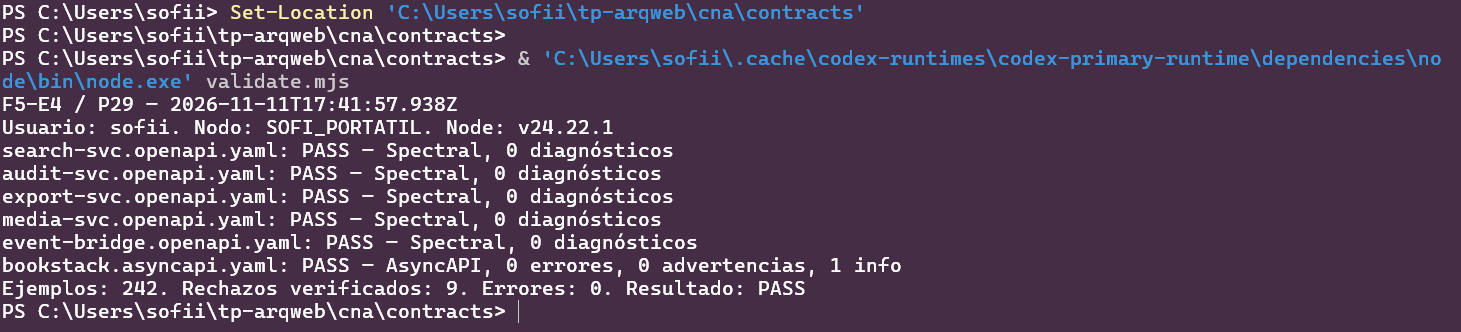
\includegraphics[width=\textwidth,height=0.6\textheight,keepaspectratio]{../../../cna/docs/evidencias/fase5/F5-E4-validacion-contratos.png}
\caption{F5-E4. Ejecución de los validadores de contratos con identificación del equipo y resultado final.}
\label{fig:f5-e4-validacion}
\end{figure}
}{}

Los contratos, el versionado y sus salidas de validación constituyen el
producto de diseño A3. La implementación de los endpoints, la durabilidad
del puente, el alcance de autorización y las interacciones se verificarán
en la Fase 6 conforme a estas especificaciones.
\endgroup

% !TeX root = main.tex
\clearpage
\subsection{A4: Modelo C4 y diagramas de secuencia}
\label{sec:fase5-a4}

\subsubsection{Alcance, niveles y estado del diseño}

El modelo representa la solución completa de BookStack CNA y desarrolla
la evolución de la arquitectura de la Figura~\ref{fig:arquitectura_logica}.
La figura original conserva la línea base del TP I; las nuevas vistas describen
el objetivo de integración del TP II. Se contrastaron las interacciones de la
sección 3.4, los requisitos de A4 y las pruebas P30--P32 de la consigna.

En C4, el nivel 1 muestra personas y sistemas; el nivel 2 abre el sistema
en aplicaciones y almacenes. Un contenedor C4 es una unidad de ejecución o
persistencia y no necesariamente un contenedor Docker. BookStack con PHP-FPM
y MariaDB pertenecen al nivel 2 aunque continúen como servicios del sistema
operativo. Las agrupaciones por VM añaden la ubicación prevista que solicita
el trabajo sin convertir el contexto de nivel 1 en un inventario de procesos.

\textbf{Estado: arquitectura objetivo de Fase 5.} El monolito de VM-1 y SSH
por su interfaz Solo host están verificados. VM-2, Swarm, microservicios,
almacenes nuevos y observabilidad se representan como diseño pendiente de
implementación. No se atribuye funcionamiento real a los flujos por haberlos
dibujado. Al finalizar Fase 6 se cotejarán estas vistas con los servicios,
puertos, reglas de red, volúmenes y versiones efectivamente desplegados.

Las decisiones proceden de ADR-006 a ADR-010 y de los contratos de A3.
El sistema en estudio abarca tanto el monolito como su extensión CNA:
BookStack no se modela como un sistema externo de esta misma plataforma.
El nivel 2 se presenta en dos láminas complementarias para distinguir el
flujo funcional de la telemetría; no son dos arquitecturas distintas.

\subsubsection{C4 nivel 1: contexto}

La Figura~\ref{fig:a4-c4-contexto} identifica al editor o lector, al consumidor
de API y al operador. Los primeros utilizan HTTPS en el gateway; el operador
administra los nodos y consulta paneles por la red privada. La caja central
resume el propósito de la plataforma y su frontera de responsabilidad.

\begin{figure}[H]
\centering
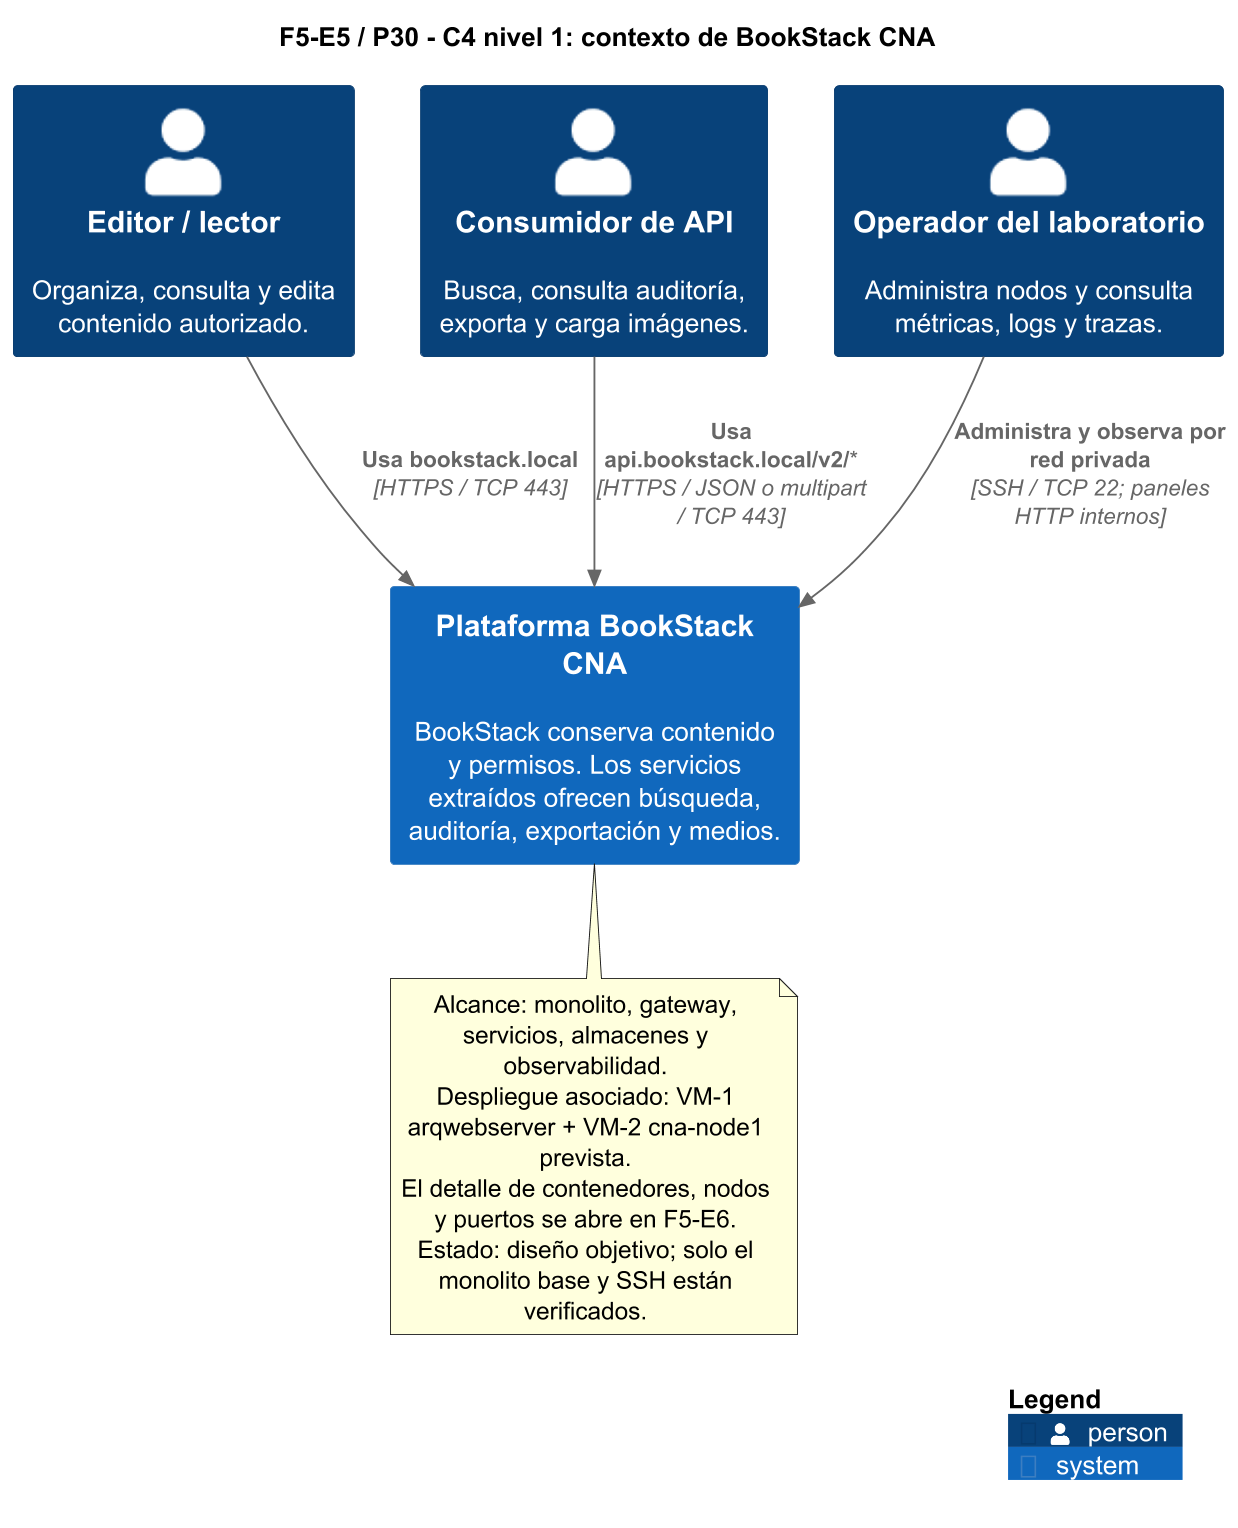
\includegraphics[width=0.71\textwidth,height=0.65\textheight,keepaspectratio]{../../../cna/docs/evidencias/fase5/a4/F5-E5-c4-contexto.png}
\caption{F5-E5 / P30. C4 nivel 1: actores y contexto de la plataforma BookStack CNA.}
\label{fig:a4-c4-contexto}
\end{figure}

\clearpage
\subsubsection{C4 nivel 2: aplicaciones, datos y operación}

Las Figuras~\ref{fig:a4-c4-contenedores} y~\ref{fig:a4-c4-operacion}
agregan nodos, protocolos y puertos. VM-1 conserva Nginx, PHP-FPM y MariaDB;
se prevé manager Swarm en \texttt{drain}. VM-2 alojará servicios, workers,
puente, broker, persistencia y observabilidad. Antes se medirá RAM y se
fijarán límites; asignar 4 GB no demuestra capacidad.

S1, S2 y el puente usan bases y roles exclusivos en PostgreSQL. S3 usa Redis
y MinIO; S4, su propio bucket. NATS distribuye eventos y no duplica la cola
ejecutable de S3. Los servicios no acceden a MariaDB.

La vista operativa incluye Prometheus, Grafana, Loki, Collector, Jaeger,
exporters y un agente de logs en VM-1. Repite referencias de la primera
lámina, sin duplicar contenedores. No supone OTLP nativo en Nginx;
la instrumentación de Webhooks se verificará sin cambiar el código del monolito.

\begin{table}[H]
\centering\small
\begin{tabularx}{\textwidth}{>{\raggedright\arraybackslash}p{3.5cm} >{\raggedright\arraybackslash}p{4.3cm} X}
\toprule
\textbf{Tramo} & \textbf{Protocolo y puerto} & \textbf{Alcance} \\
\midrule
Cliente--gateway & HTTPS/TCP 443; HTTP 80 para redirección & Entrada web; dominios del monolito y de API. \\
Operador--nodos & SSH/TCP 22 & Solo host; VM-1 verificada, VM-2 prevista. \\
Gateway--BookStack & FastCGI por socket Unix & Local en VM-1; ruta efectiva a cotejar. \\
BookStack--MariaDB & Socket local o TCP 3306 local & Transporte efectivo a verificar; sin acceso de servicios. \\
Gateway--S1/S2/S3/S4 & HTTP 8081/8082/8083/8084 hacia 8000 & Publicación privada \texttt{mode=host} propuesta. \\
BookStack--puente & HTTP 8085 hacia 8000 & Webhook y token; red privada. \\
Servicios--almacenes & SQL 5432; RESP 6379; NATS 4222; S3 HTTP 9000 & Red interna; credenciales y propiedad separadas. \\
Swarm entre nodos & TCP 2377; TCP/UDP 7946; UDP 4789 & Solo nodos privados; ESP si se cifra overlay. \\
\bottomrule
\end{tabularx}
\caption{Puertos funcionales propuestos en A4. No representan un relevamiento de sockets ni reglas de firewall ya aplicadas.}
\label{tab:a4-puertos}
\end{table}

Los puertos de telemetría y sus restricciones se detallan en la vista
operativa y en la tabla completa junto a las fuentes. VM-1 conserva
\texttt{192.168.145.129} en \texttt{ens37}; \texttt{ens33} usa DHCP.
La IP privada de VM-2 está pendiente. Un manager, un broker y volúmenes
locales no constituyen alta disponibilidad.

\clearpage
\begin{landscape}
\pdfpageattr{/Rotate 90}
\begin{figure}[p]
\centering
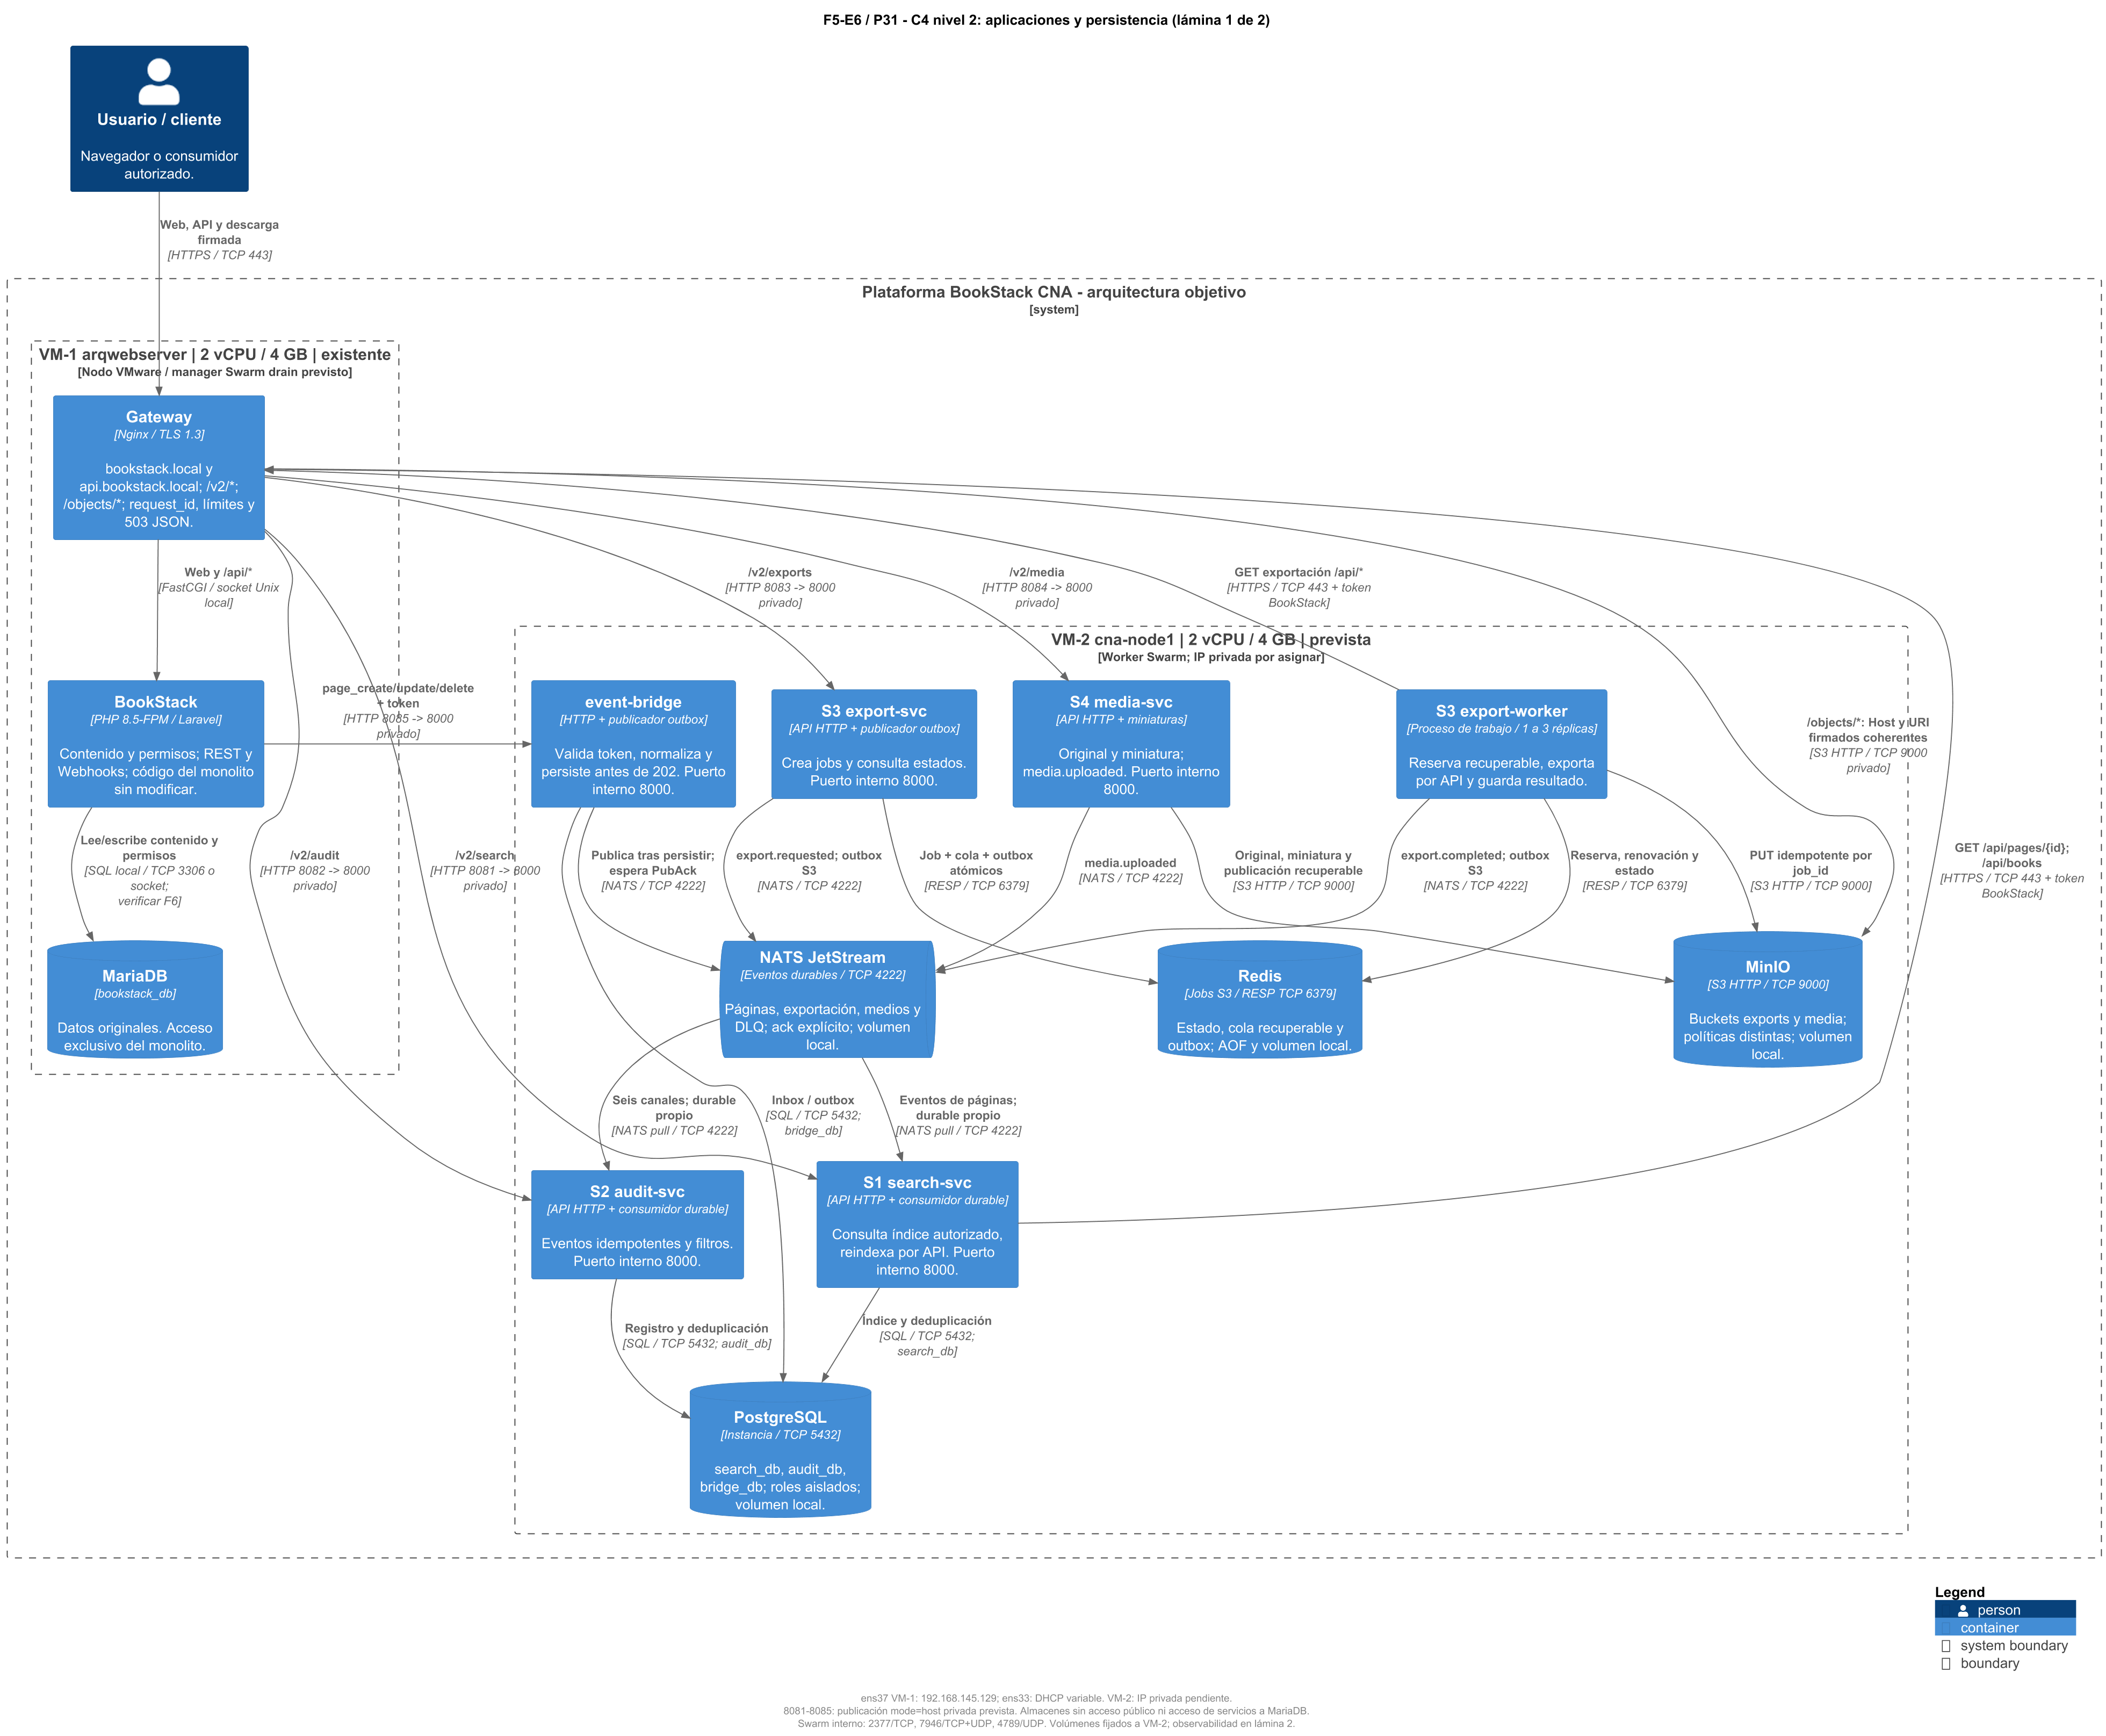
\includegraphics[width=\linewidth,height=0.86\textheight,keepaspectratio]{../../../cna/docs/evidencias/fase5/a4/F5-E6-01-c4-contenedores.png}
\caption{F5-E6 / P31. C4 nivel 2, lámina 1: aplicaciones, persistencia, nodos y comunicaciones de la arquitectura objetivo.}
\label{fig:a4-c4-contenedores}
\end{figure}
\clearpage
\begin{figure}[p]
\centering
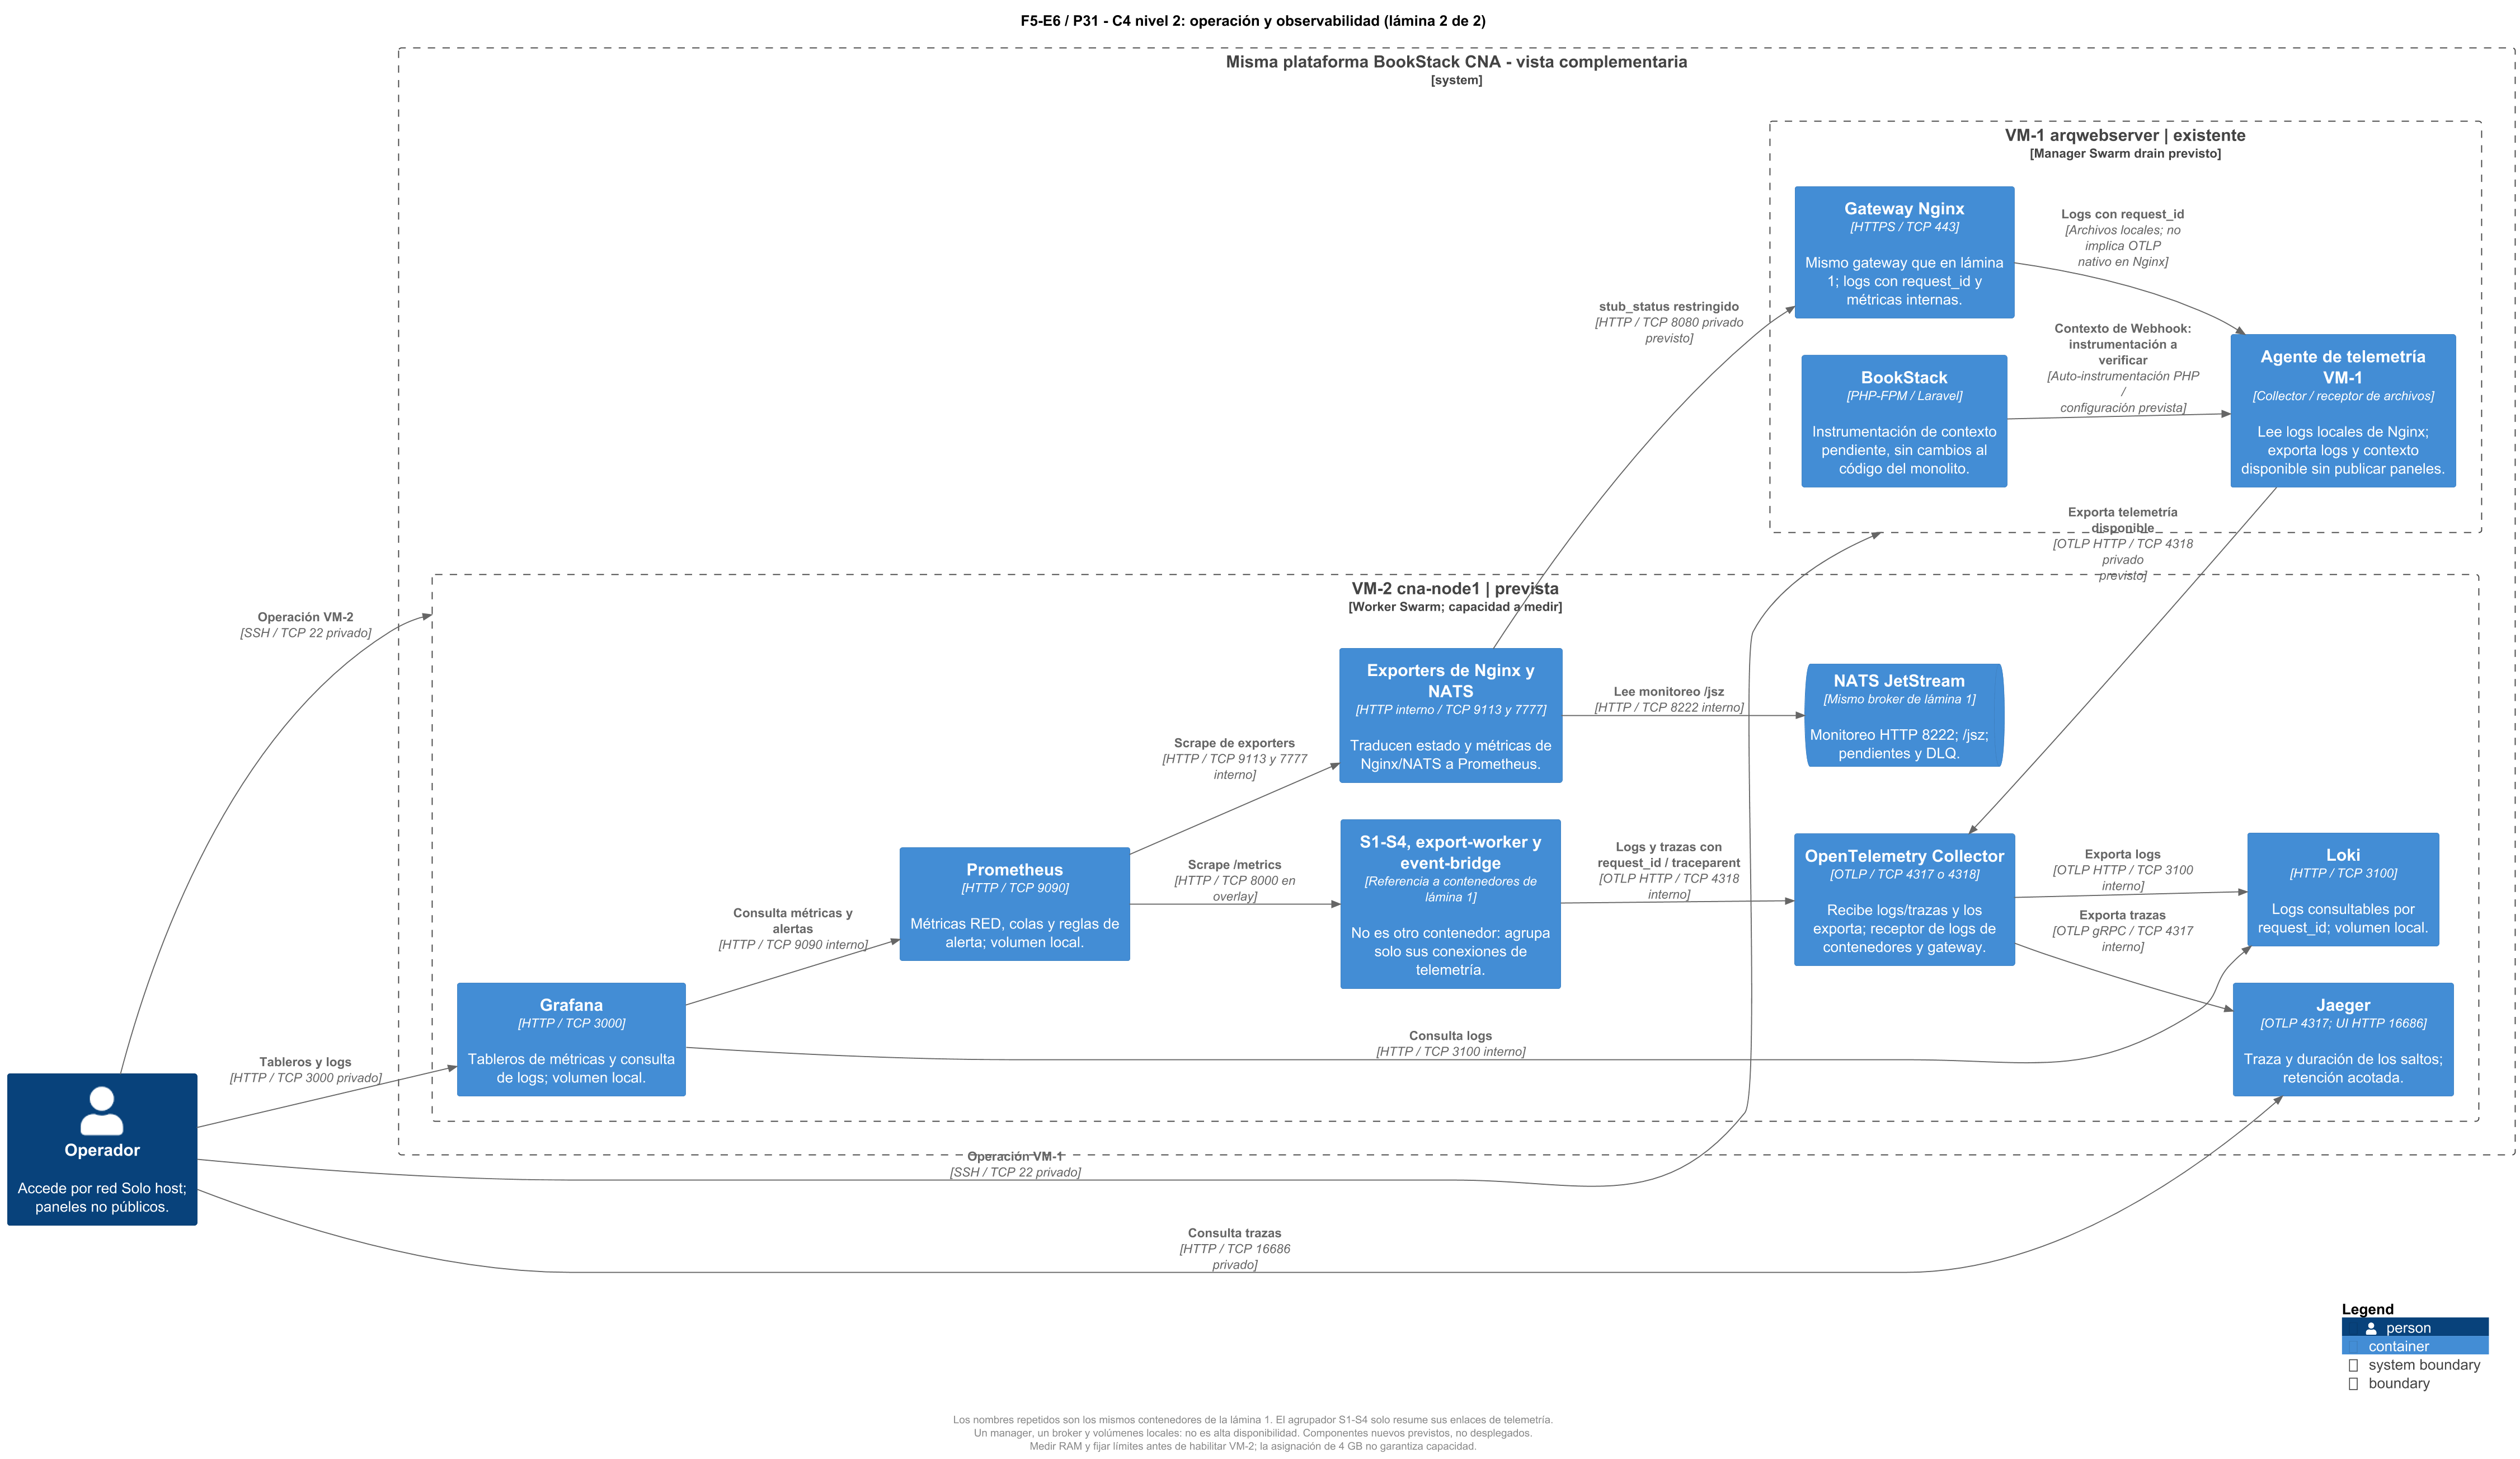
\includegraphics[width=\linewidth,height=0.86\textheight,keepaspectratio]{../../../cna/docs/evidencias/fase5/a4/F5-E6-02-c4-operacion.png}
\caption{F5-E6 / P31. C4 nivel 2, lámina 2: administración, métricas, logs y trazas previstas, complementarias a la lámina funcional.}
\label{fig:a4-c4-operacion}
\end{figure}
\clearpage
\end{landscape}
\pdfpageattr{}

\subsubsection{Tres secuencias y sus caminos de error}

Cada diagrama corresponde a una interacción obligatoria de la sección 3.4.
Se lee de arriba hacia abajo; \texttt{alt} separa alternativas y \texttt{par}
representa consumidores independientes. Edición y exportación se dividen
en dos láminas cada una para conservar legibilidad. Se mantienen tres
interacciones lógicas, no cinco casos diferentes.

\paragraph{Edición, indexación y auditoría.}
Las Figuras~\ref{fig:a4-edicion} y~\ref{fig:a4-edicion-error} siguen la edición,
el Webhook y la aceptación persistente del puente. La publicación espera
confirmación de JetStream. S1 obtiene contenido autorizado por la API y
guarda índice y deduplicación en una transacción; S2 registra el mismo evento
en su propia base. Ambos reconocen después de guardar sus efectos.
Los errores cubren entrada inválida, persistencia o broker caídos,
timeout hacia BookStack, reentrega, consumidor detenido y traslado confirmado
a DLQ. La meta de indexación menor que cinco segundos requiere medición real.

El código relevado no reprograma el Webhook si nunca llega al puente.
La recuperación del índice por API no reconstruye por sí sola la auditoría
perdida. Además, el Webhook no hereda automáticamente el identificador de la
edición: si falta, el puente inicia otra correlación. Estas limitaciones
quedan visibles y requieren tratamiento y prueba en las siguientes fases.

\paragraph{Búsqueda síncrona.}
La Figura~\ref{fig:a4-busqueda} recorre cliente, gateway, S1 e índice propio.
Incluye validación, autorización, respuesta 200 y enlaces al monolito.
Sin coincidencias devuelve una lista vacía con 200. Los caminos de error
incluyen 400, 401/403, 429 y 503 por S1 o base inaccesibles. El gateway debe
convertir los fallos del upstream al error JSON acordado y conservar
\texttt{X-Request-ID}; la consulta no accede a MariaDB.

\paragraph{Exportación por trabajos.}
Las Figuras~\ref{fig:a4-exportacion} y~\ref{fig:a4-exportacion-error}
recorren el 202 y su \texttt{job\_id}, reserva recuperable, exportación por API,
objeto en MinIO, estado \texttt{done} y descarga firmada mediante el gateway.
Los errores incluyen conflicto de clave idempotente, Redis no disponible
antes de aceptar, API o almacenamiento fallidos y caída del worker.
Un job fallido conocido se consulta con 200 y estado \texttt{failed}.
La publicación pendiente se conserva en outbox si NATS falla. Redis AOF
y volúmenes requieren validar su política real de persistencia; no se
presentan como una garantía de pérdida cero ante cualquier caída.

\clearpage
\begin{figure}[p]
\centering
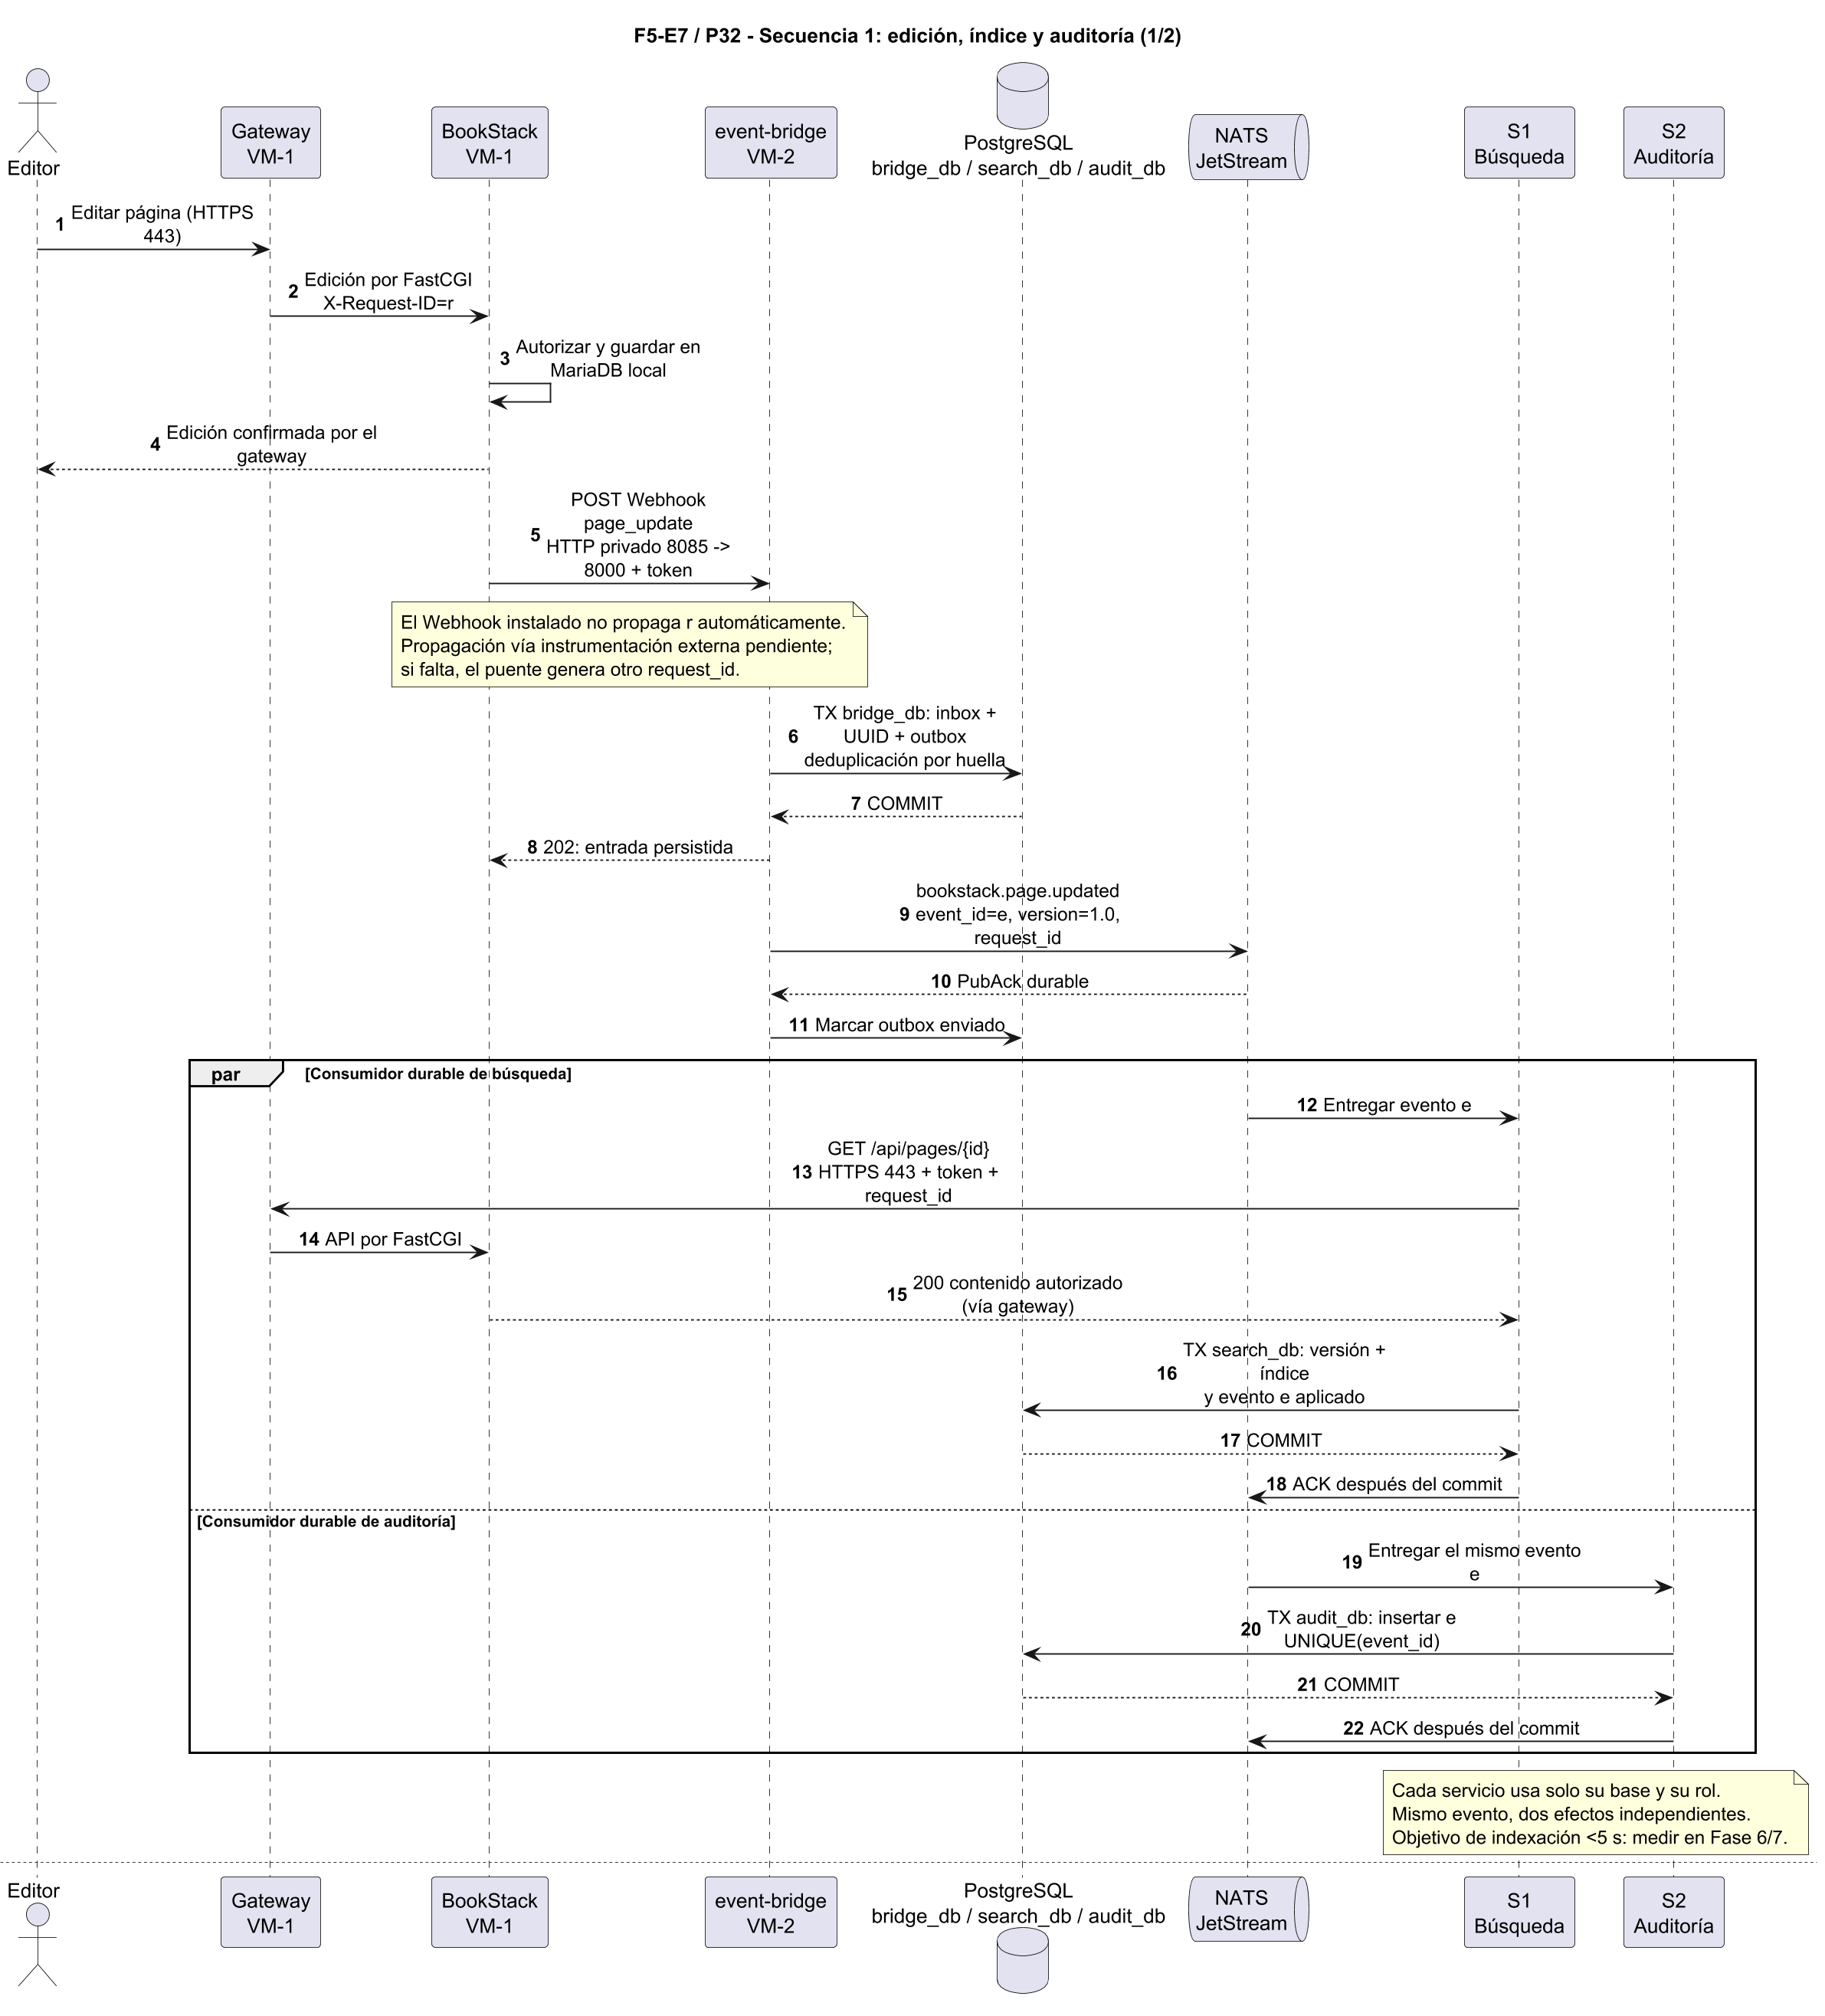
\includegraphics[width=\textwidth,height=0.88\textheight,keepaspectratio]{../../../cna/docs/evidencias/fase5/a4/F5-E7-01-edicion-indexacion.png}
\caption{F5-E7 / P32. Secuencia 1, lámina principal: edición, aceptación persistente, indexación y auditoría independientes.}
\label{fig:a4-edicion}
\end{figure}
\clearpage
\begin{figure}[p]
\centering
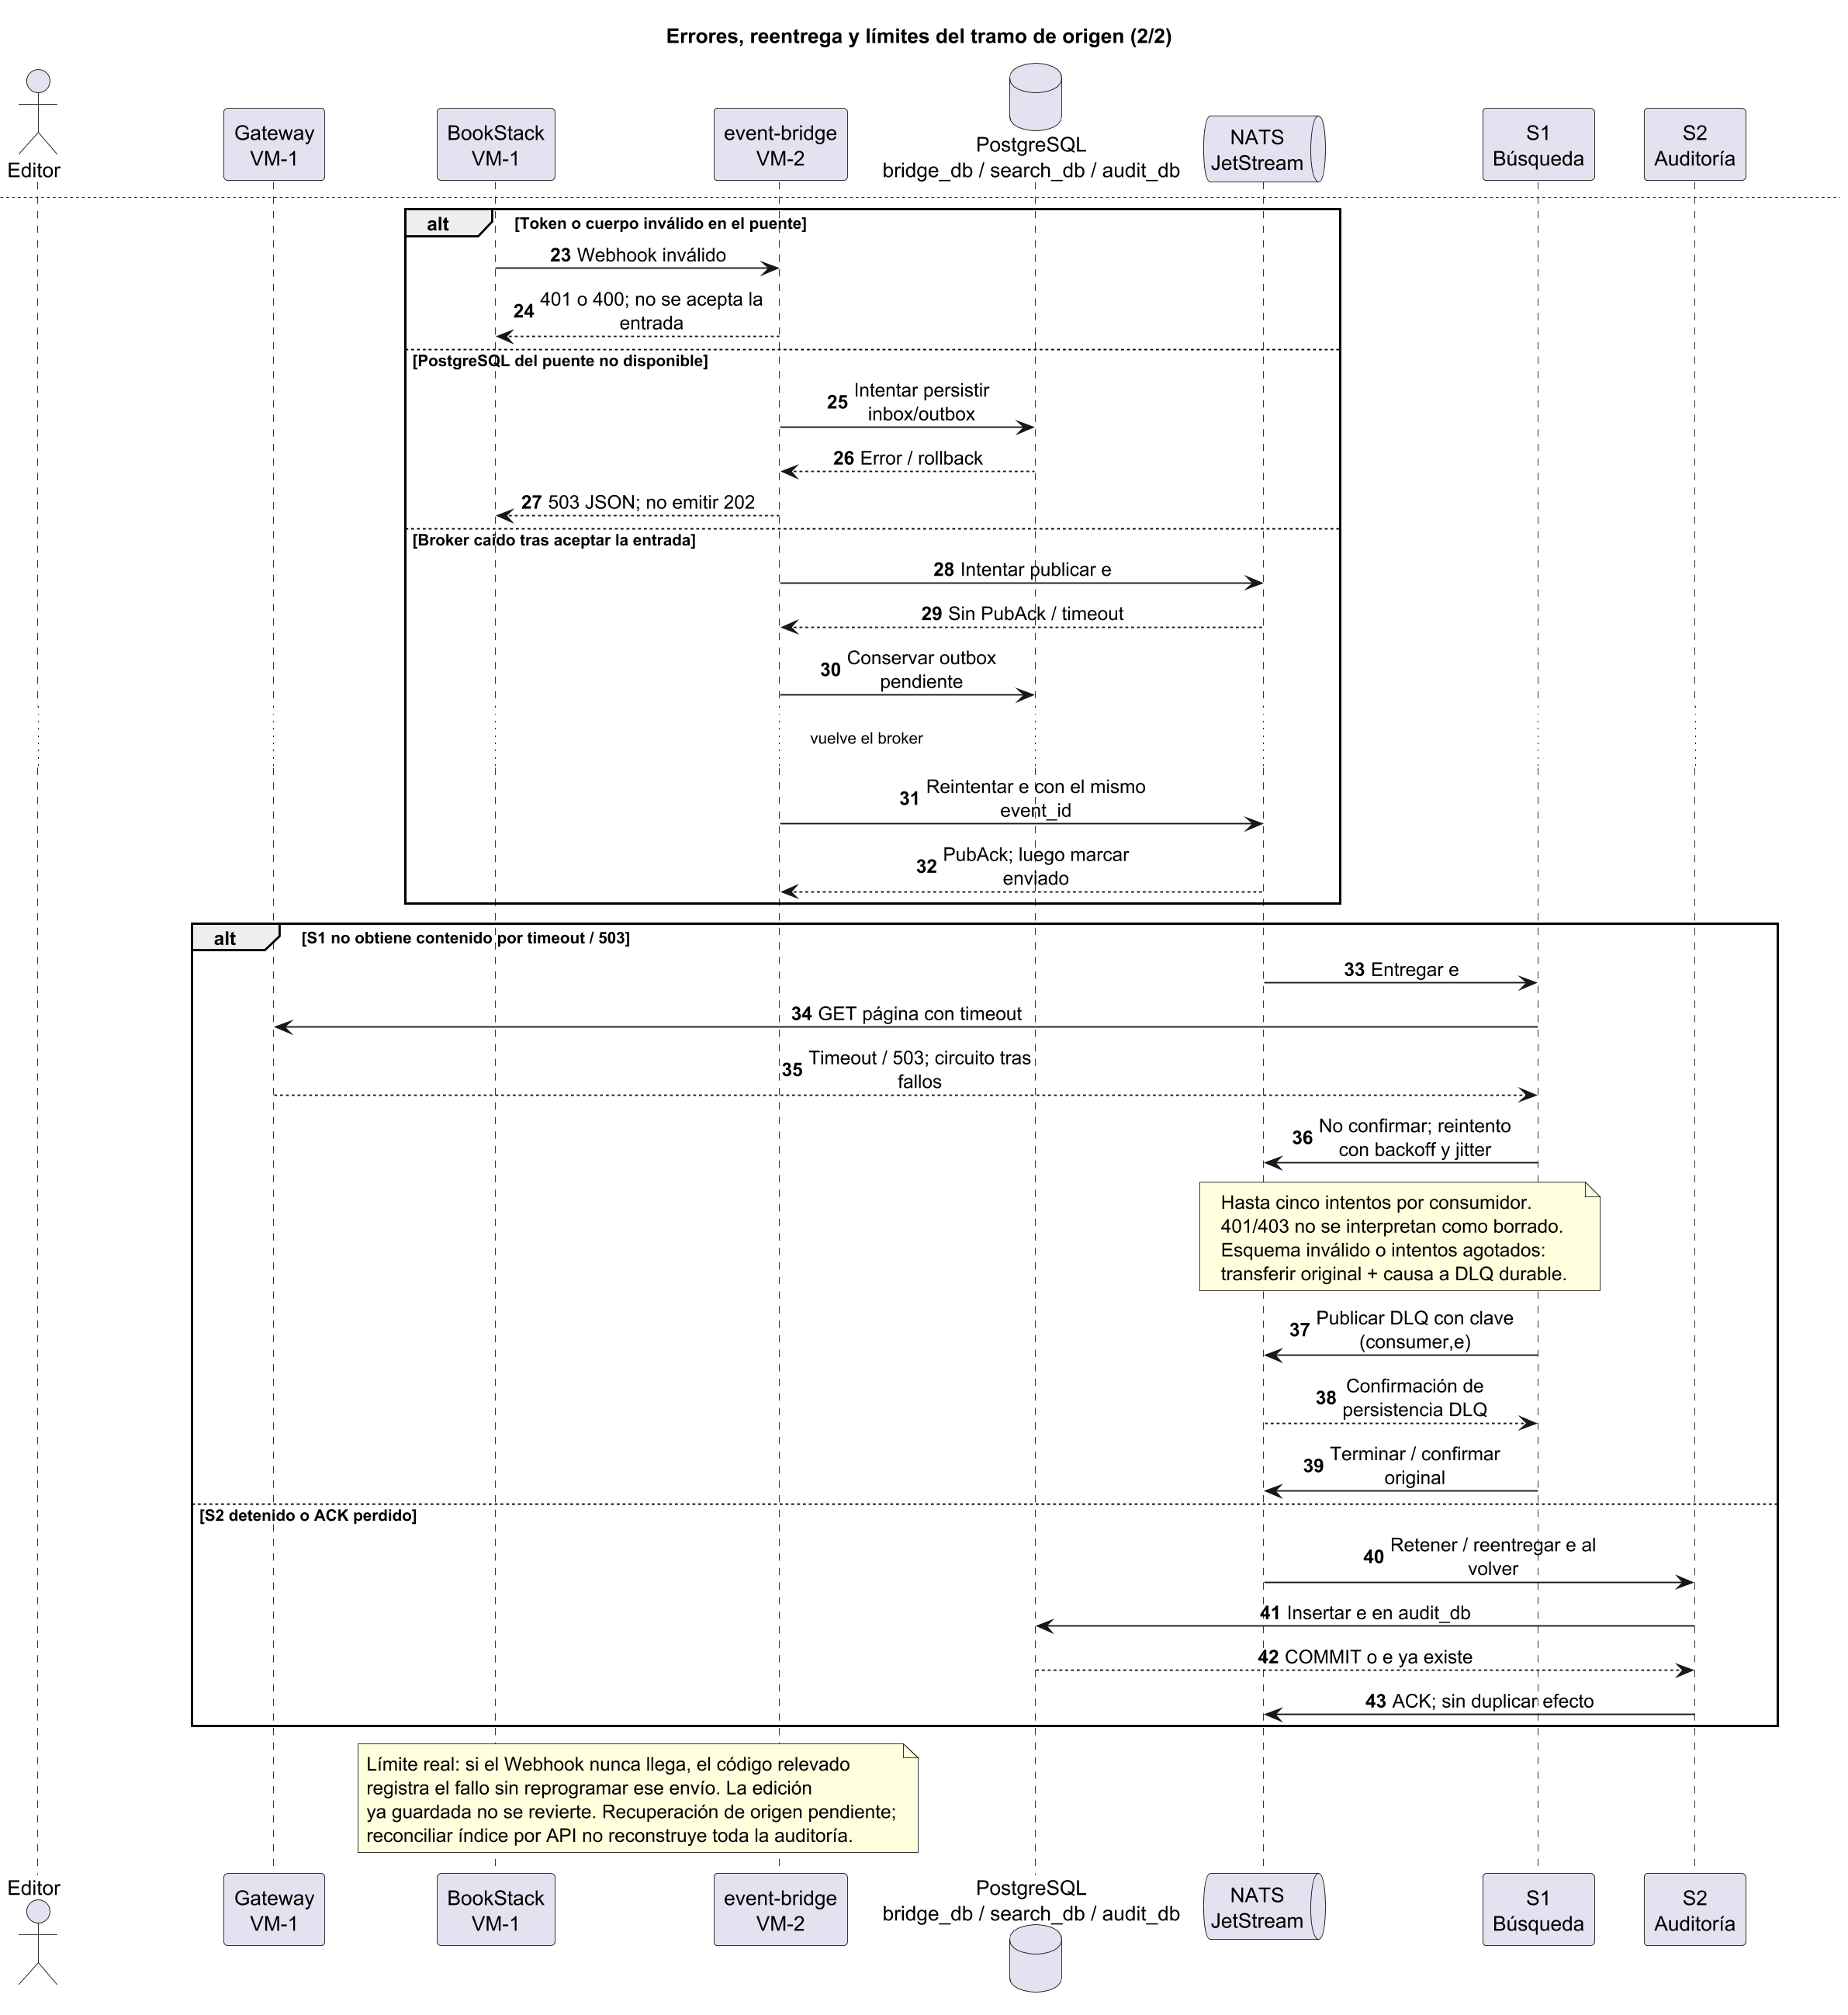
\includegraphics[width=\textwidth,height=0.88\textheight,keepaspectratio]{../../../cna/docs/evidencias/fase5/a4/F5-E7-01-edicion-indexacion_001.png}
\caption{F5-E7 / P32. Secuencia 1, errores y recuperación: outbox, reintentos, DLQ, reentrega y límite de recuperación del Webhook de origen.}
\label{fig:a4-edicion-error}
\end{figure}
\clearpage
\begin{figure}[p]
\centering
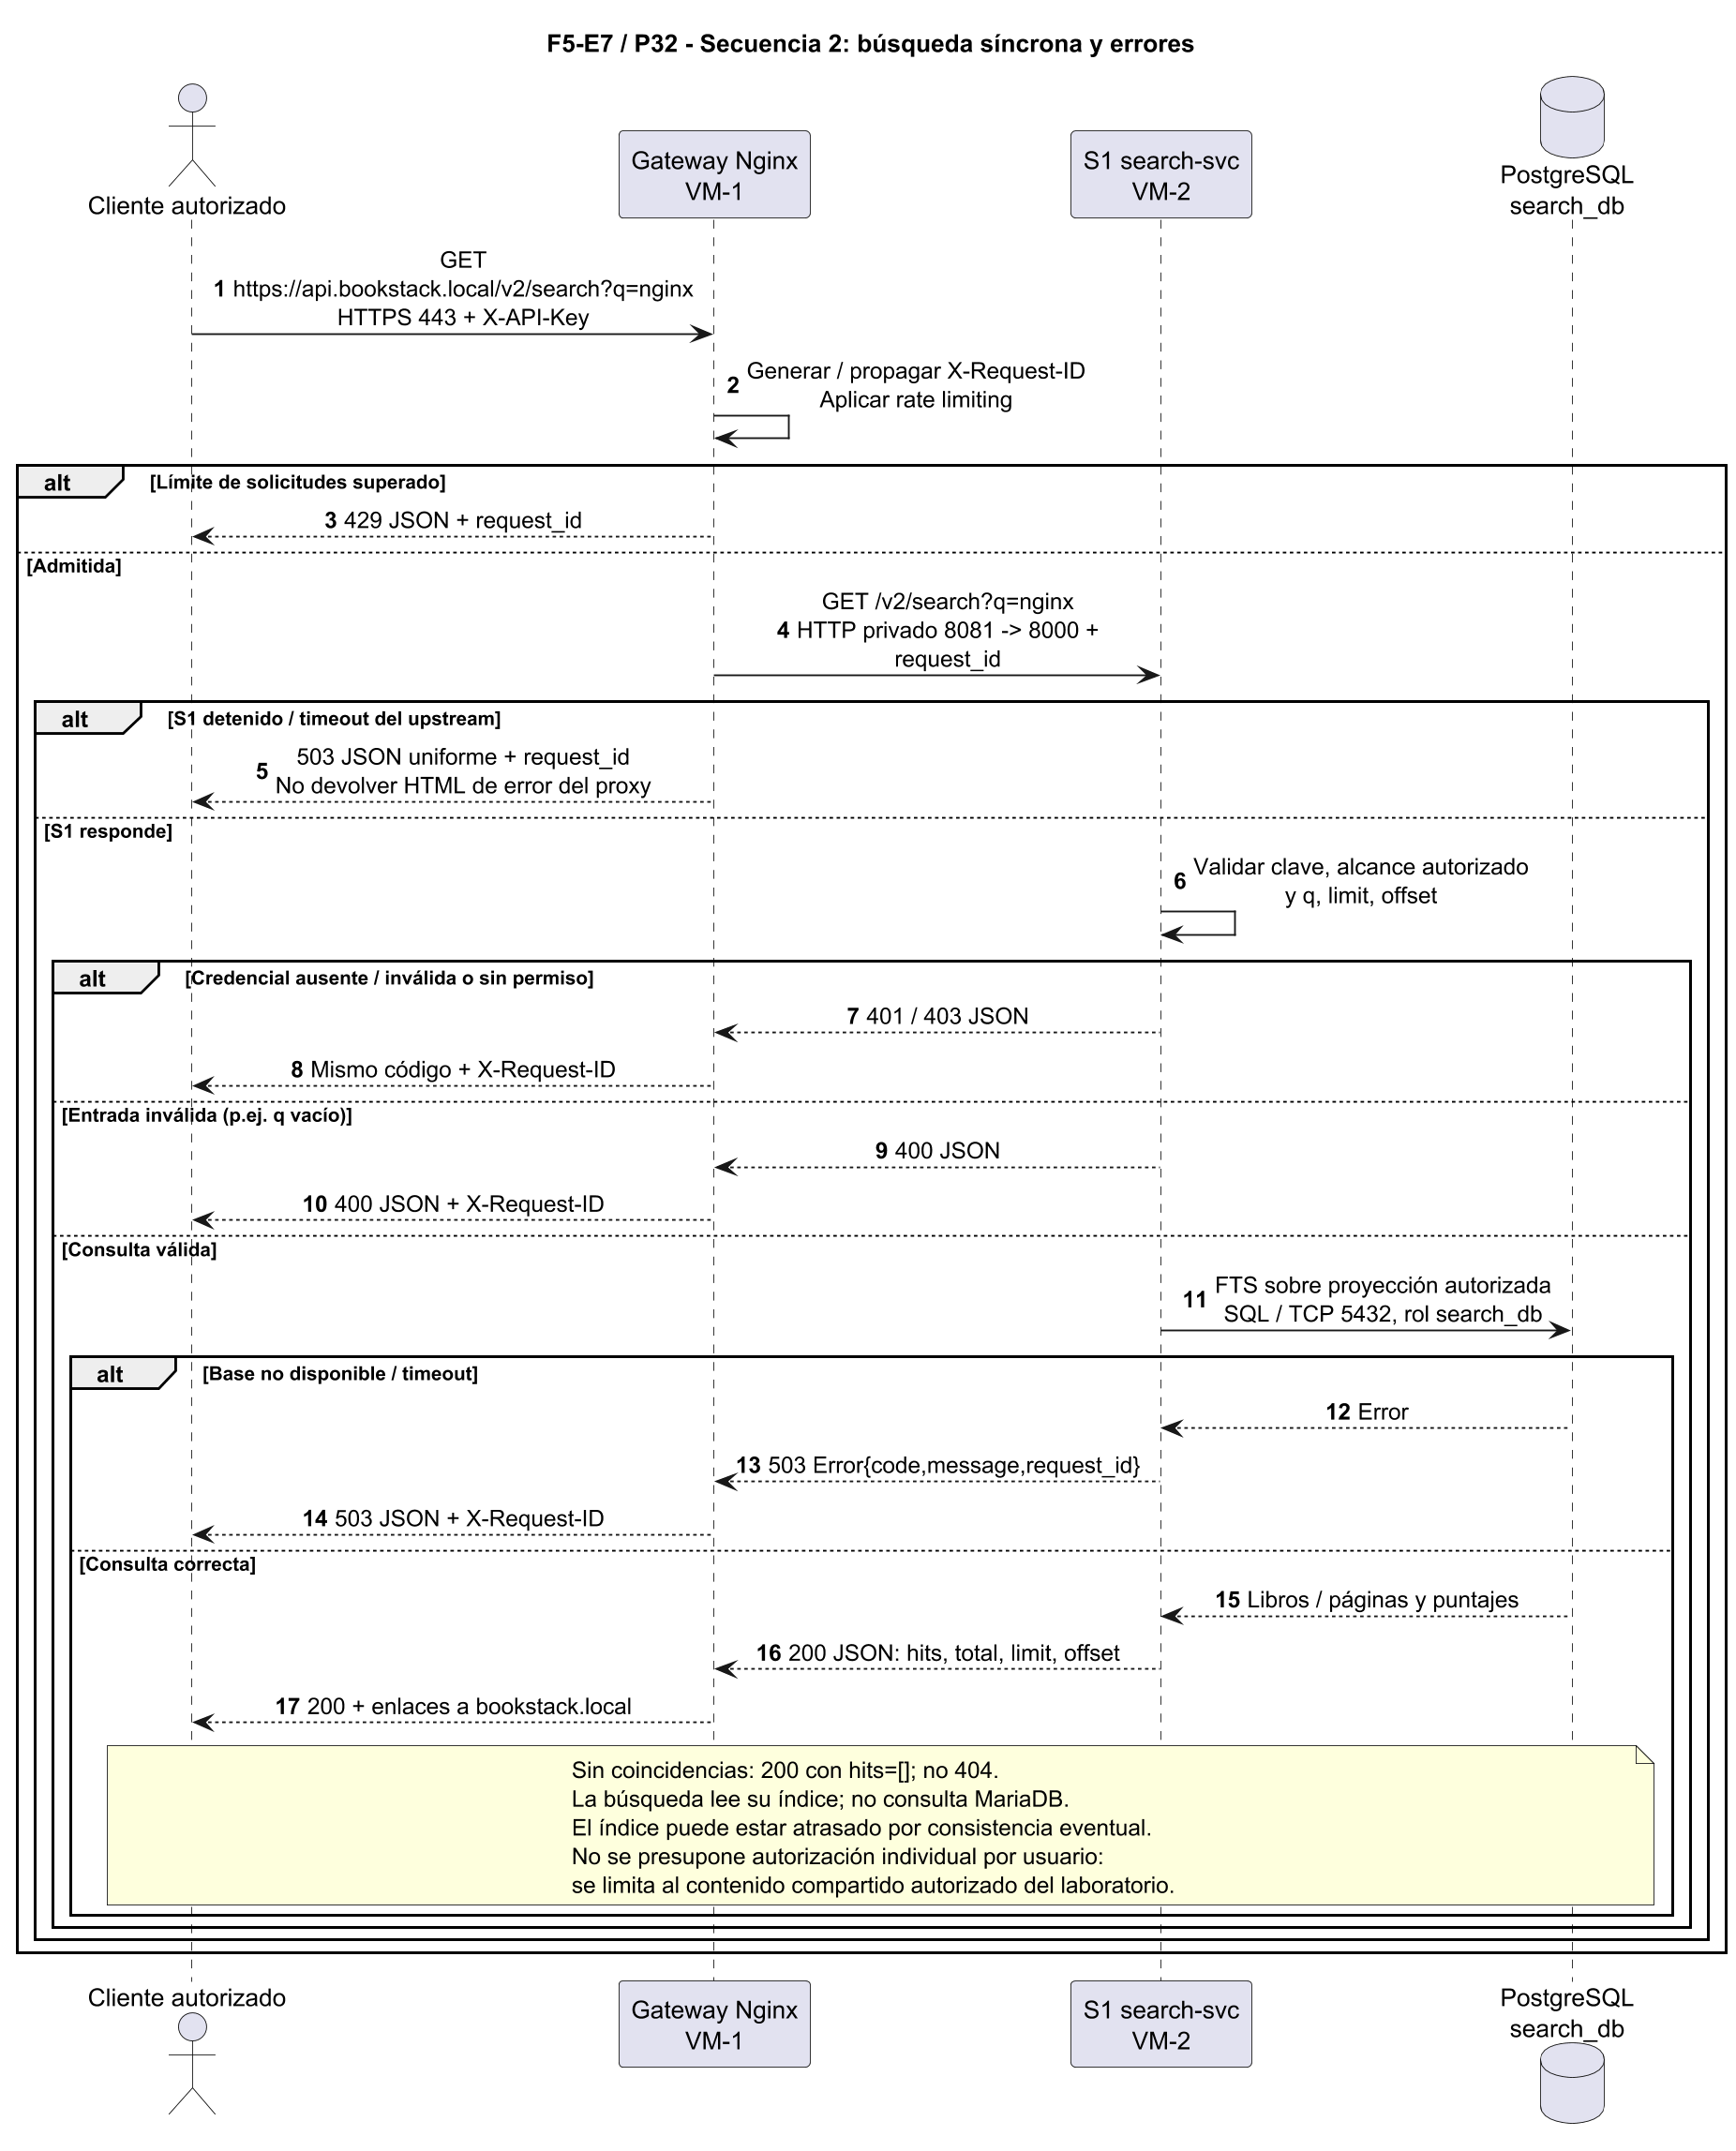
\includegraphics[width=\textwidth,height=0.88\textheight,keepaspectratio]{../../../cna/docs/evidencias/fase5/a4/F5-E7-02-busqueda.png}
\caption{F5-E7 / P32. Secuencia 2: búsqueda síncrona, respuesta normal, validaciones y caminos de error de gateway, servicio e índice.}
\label{fig:a4-busqueda}
\end{figure}
\clearpage
\begin{figure}[p]
\centering
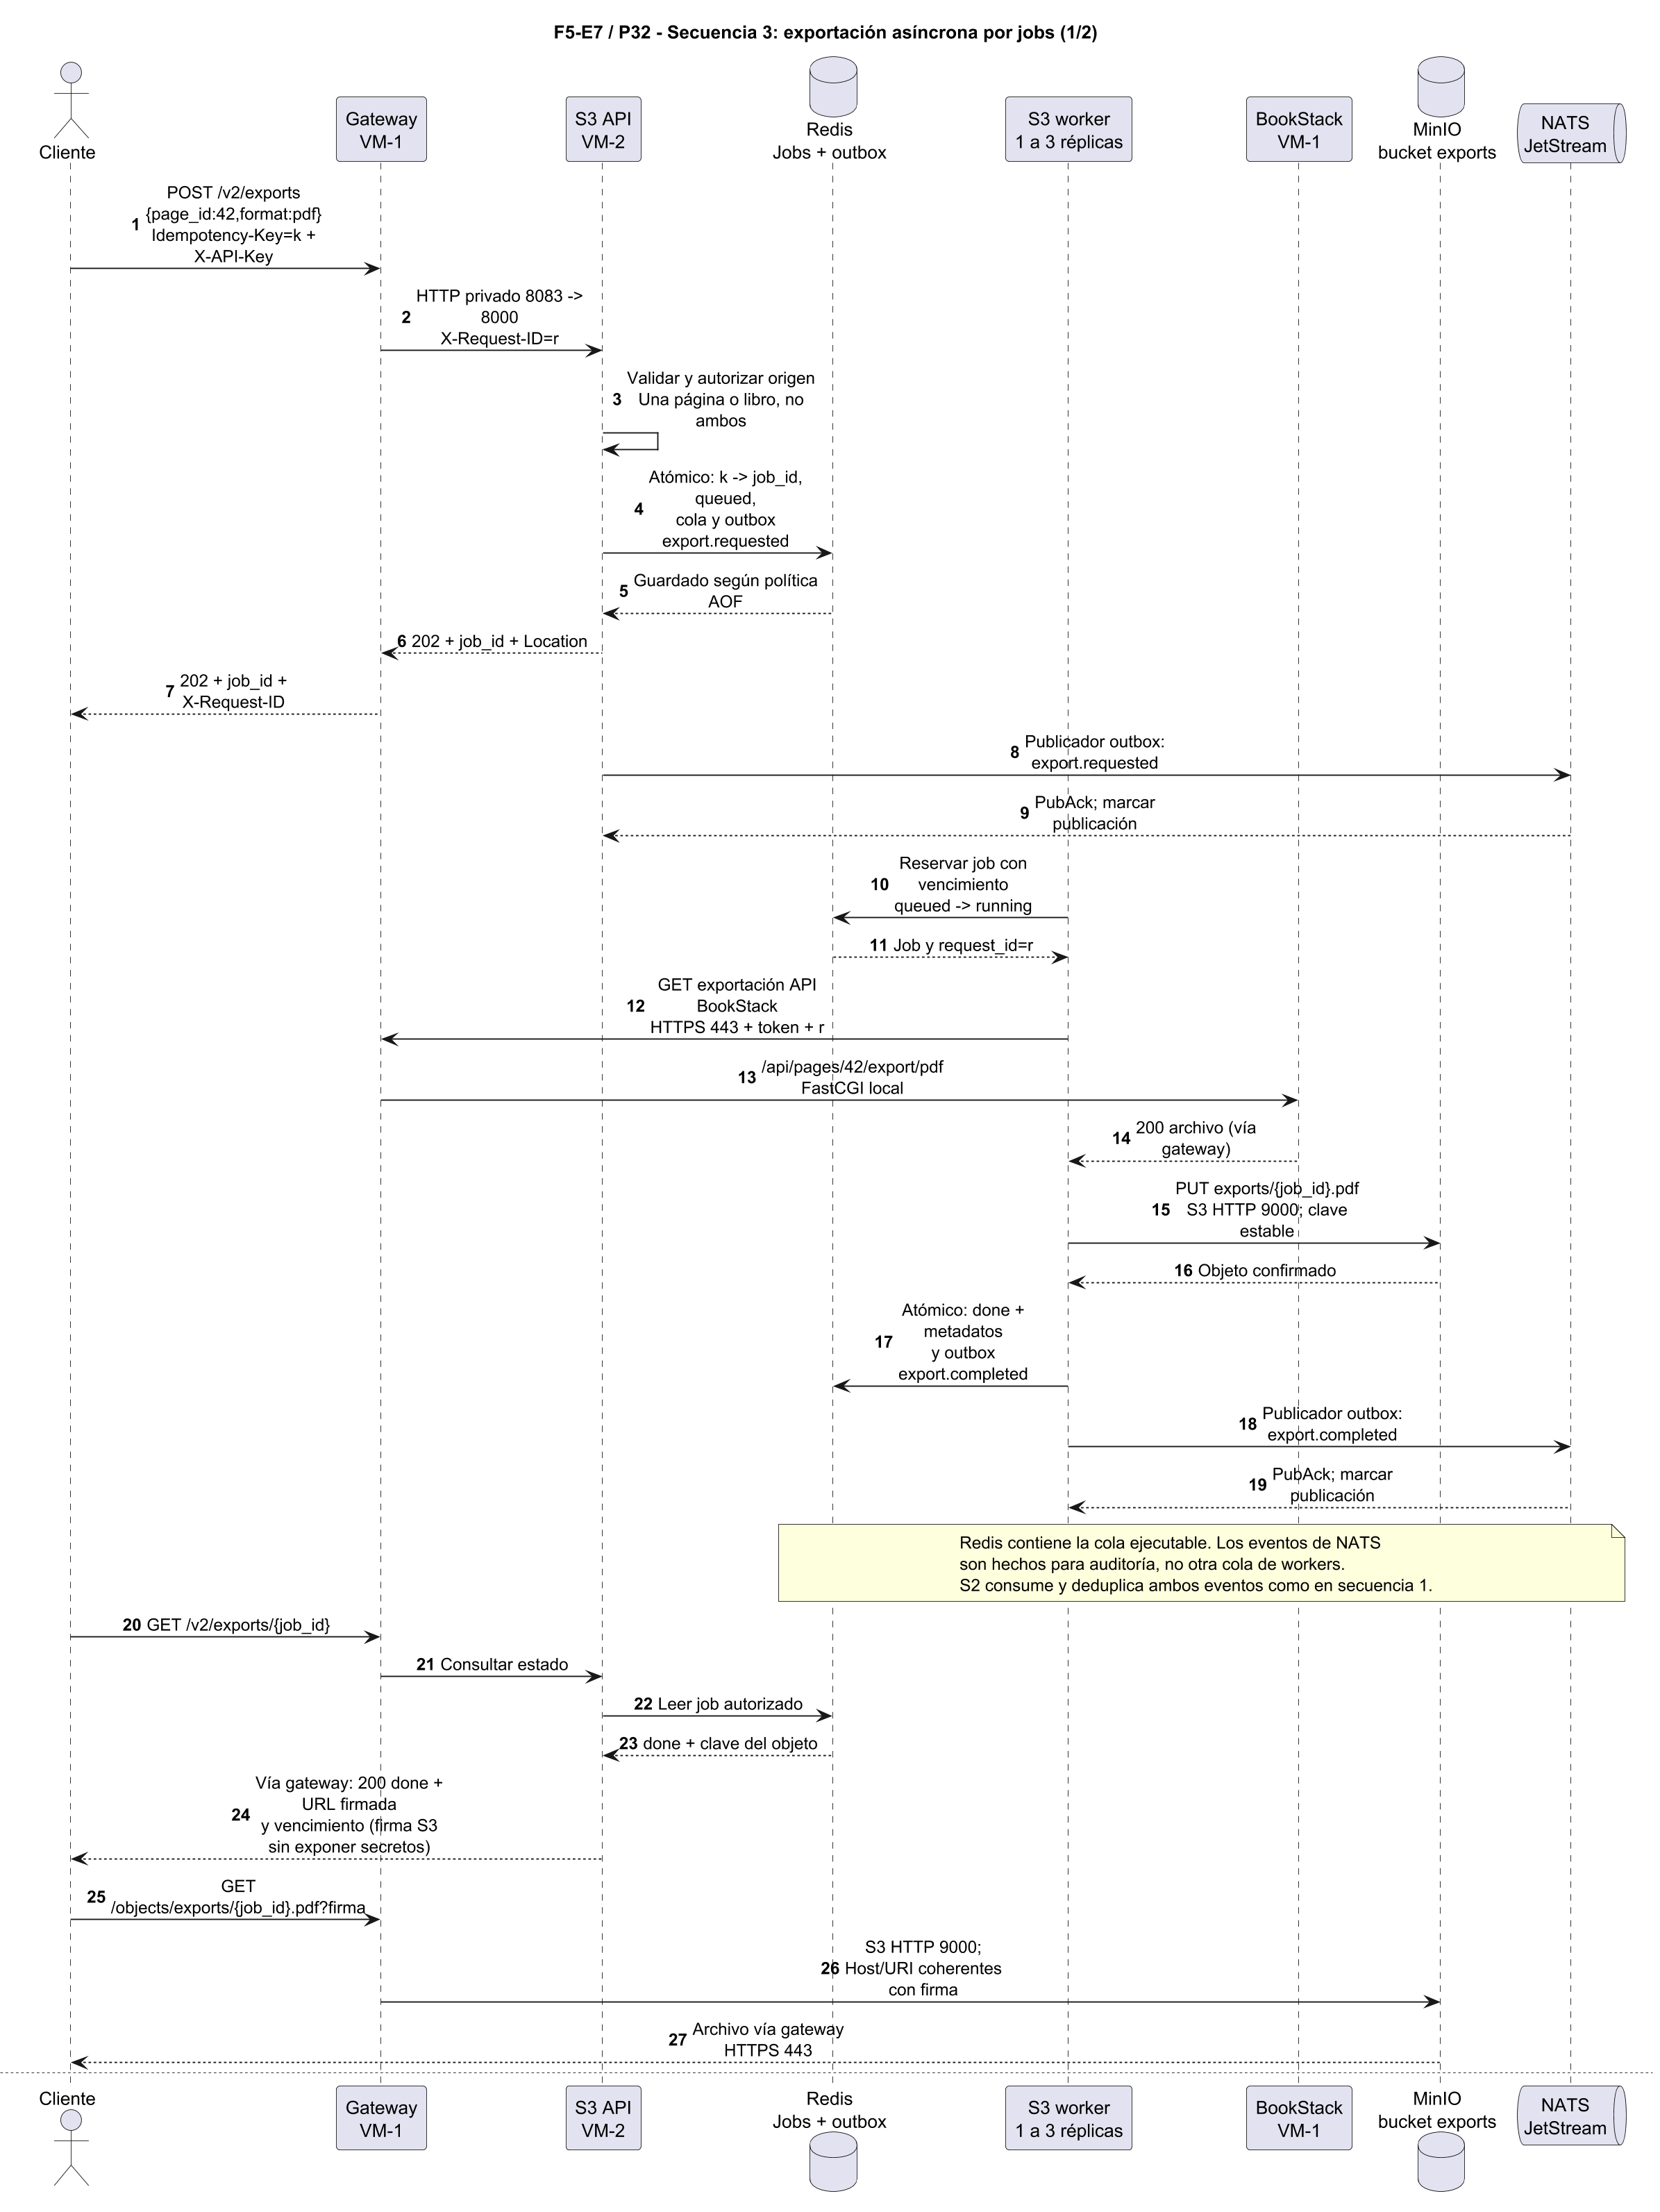
\includegraphics[width=\textwidth,height=0.88\textheight,keepaspectratio]{../../../cna/docs/evidencias/fase5/a4/F5-E7-03-exportacion.png}
\caption{F5-E7 / P32. Secuencia 3, lámina principal: job asíncrono, worker, exportación por API y descarga del objeto mediante URL firmada.}
\label{fig:a4-exportacion}
\end{figure}
\clearpage
\begin{figure}[p]
\centering
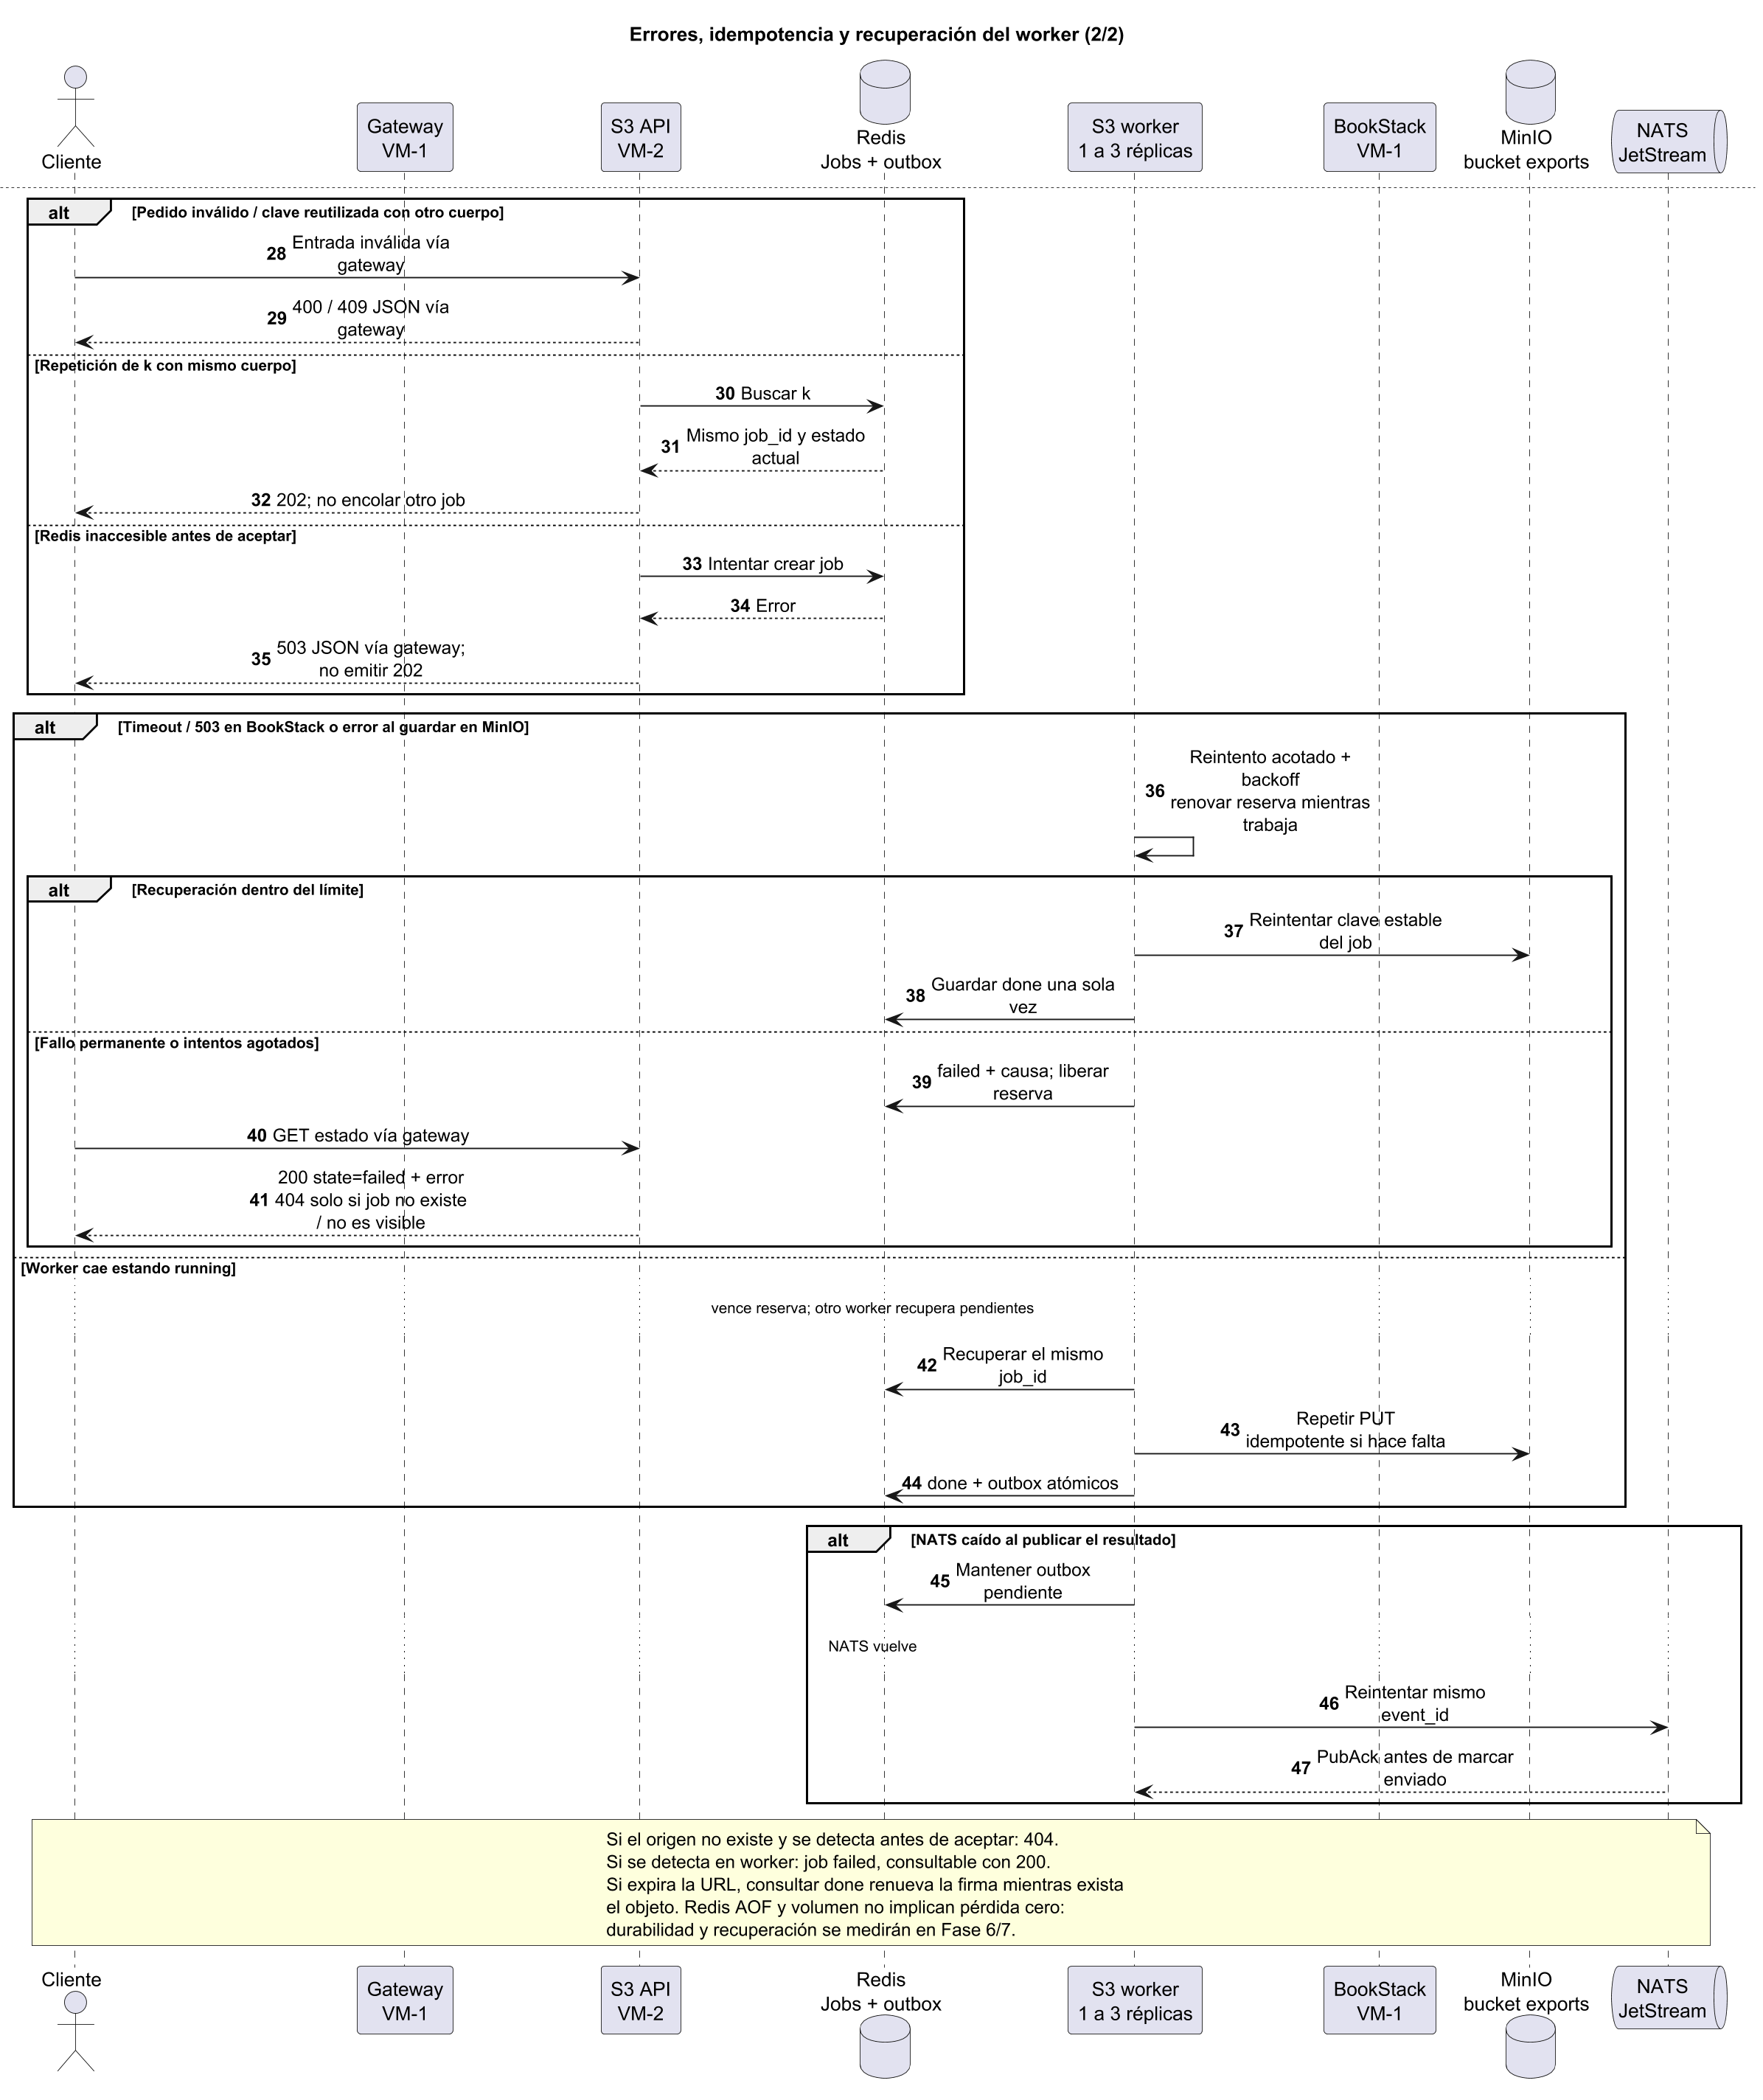
\includegraphics[width=\textwidth,height=0.88\textheight,keepaspectratio]{../../../cna/docs/evidencias/fase5/a4/F5-E7-03-exportacion_001.png}
\caption{F5-E7 / P32. Secuencia 3, errores y recuperación: idempotencia, aceptación condicionada, fallo del worker y publicación recuperable.}
\label{fig:a4-exportacion-error}
\end{figure}
\clearpage

\subsubsection{Fuentes, evidencias y verificación de A4}

Las seis fuentes PlantUML se conservan en
\path{cna/docs/diagramas/a4/}: un contexto, dos vistas del mismo nivel 2 y
tres secuencias. PlantUML 1.2025.10 incluye la biblioteca C4 utilizada;
el script \texttt{renderizar.ps1} comprueba el hash de la herramienta,
la sintaxis y la generación de ocho láminas PNG y ocho SVG. Los SVG conservan
líneas y texto al ampliar y acompañan las imágenes del informe.

Las evidencias y los reportes de compilación se guardan en
\path{cna/docs/evidencias/fase5/a4/}. El JSON registra fecha, nodo, versión
de herramienta y SHA-256 de fuentes y resultados. La revisión visual
comprueba que participantes, alternativas y etiquetas sean legibles y no
estén recortados; la revisión de coherencia contrasta nodos, propiedad de
datos y mensajes con A2 y A3. No constituye una prueba de los servicios.

\begin{table}[H]
\centering\small
\begin{tabularx}{\textwidth}{>{\raggedright\arraybackslash}p{1.3cm} >{\raggedright\arraybackslash}p{1.9cm} X}
\toprule
\textbf{Prueba} & \textbf{Evidencia} & \textbf{Producto de diseño verificado} \\
\midrule
P30 & F5-E5 & C4 nivel 1 con actores, frontera del sistema y accesos. \\
P31 & F5-E6 & Nivel 2 con aplicaciones, almacenes, nodos y puertos/protocolos; vista operativa complementaria. \\
P32 & F5-E7 & Tres interacciones obligatorias, con caminos normales y de error, correlación y recuperación previstas. \\
\bottomrule
\end{tabularx}
\caption{Continuación de la matriz: evidencias de diseño de A4. La comprobación contra el despliegue se realizará en Fase 6.}
\label{tab:a4-evidencias}
\end{table}

La versión de diseño cubre las piezas solicitadas en A4 y conserva las
limitaciones pendientes de implementación. Toda modificación de topología,
puertos o contratos durante la construcción deberá actualizar las fuentes,
regenerar las evidencias y recompilar el informe.

% !TeX root = main.tex
\clearpage
\subsection{A5: Plan de migración y matriz de riesgos}
\label{sec:fase5-a5}

\subsubsection{Alcance y reglas de transición}

El plan desarrolla las secciones 4.5 y 4.6 de la consigna: orden de extracción
justificado, criterio de hecho por etapa, reversión planificada en menos de
un minuto y matriz de probabilidad por impacto con mitigaciones. Se apoya
en ADR-006--010, contratos A3 y modelo A4. Las fuentes editables se conservan
en \path{cna/docs/a5/}.

BookStack conserva su código, contenido, permisos y MariaDB. La integración
se limita a REST y Webhooks; no se entregan credenciales de MariaDB a los
servicios nuevos. Se habilita una funcionalidad por vez, después de probarla
en paralelo, y se mantiene disponible su alternativa nativa. Cerrar una
entrada no implica borrar colas, eventos, trabajos ni archivos.

\textbf{Estado: plan de diseño.} Los criterios de hecho siguientes son
condiciones de salida para ejecutar en Fases 6 y 7, no pruebas aprobadas.
La duración de reversión y la recuperación de datos no se han medido.
El cierre documental de Fase 5 no equivale a cumplir los criterios globales
CA-1--CA-7 del trabajo completo.

\subsubsection{Orden de extracción y criterio de hecho}

El orden relativo es \textbf{S2 auditoría, S1 búsqueda, S3 exportación y S4
medios}. Primero se agregan registros y proyecciones sin reemplazar el
contenido; después se incorporan trabajos y objetos con referencias
duraderas. La prioridad se refiere al impacto funcional y al costo de
reversión en esta instalación. No implica que se tolere perder auditoría.

\begin{table}[H]
\centering\small
\begin{tabularx}{\textwidth}{>{\raggedright\arraybackslash}p{1.1cm} >{\raggedright\arraybackslash}p{2.7cm} >{\raggedright\arraybackslash}X}
\toprule
\textbf{Paso} & \textbf{Alcance} & \textbf{Justificación y condición de habilitación} \\
\midrule
M0 & Preparación & Proteger línea base, validar recursos, backup/restauración, red, secretos y variantes de gateway antes de abrir rutas. \\
M1 & S2 auditoría & Registro paralelo sin intervenir la edición; habilitar después de deduplicar, recuperar pendientes y probar filtros. \\
M2 & S1 búsqueda & Proyección reconstruible; abrir tras verificar autorización, reconciliación y actualización menor que 5 s. \\
M3 & S3 exportación & Jobs y objetos con efectos en curso; abrir POST después de probar reserva recuperable, estado y descarga. \\
M4 & S4 medios & Objetos potencialmente referenciados por contenido; exige retención y restauración antes de nuevas referencias. \\
M5 & Consolidación & Cotejar despliegue, criterios globales, pruebas y reversión medida antes de la entrega final. \\
\bottomrule
\end{tabularx}
\caption{Orden de migración de A5, de menor a mayor riesgo funcional, con preparación y consolidación.}
\label{tab:a5-orden}
\end{table}

\clearpage
\paragraph{M0: preparar sin alterar la línea base.}
Guardar backup consistente de base, archivos, configuración y secretos
necesarios para restaurar, fuera de Git y con acceso restringido. Probar la
restauración en un entorno aislado. Verificar RAM del anfitrión, recursos
de ambas VM, red privada, certificados y puertos; preparar límites,
variantes de gateway y probes nativos antes de habilitar VM-2.
\textbf{Hecho:} restauración evidenciada; login, creación de libro y edición
intactos; red y restricciones comprobadas; presupuesto medido y entrada del
puente persistida antes de 202, recuperable ante caída del broker.
Responsable previsto: infraestructura, con revisión de otro integrante.

\paragraph{M1: auditoría con S2.}
Crear base y rol propios y consumidor durable independiente. Contrastar
eventos aceptados con actividad nativa sin cambiar páginas.
\textbf{Hecho:} filtros de A3 correctos; un efecto por \texttt{event\_id};
S2 detenido dos minutos durante veinte ediciones recupera los veinte eventos
publicados; un mensaje inválido conserva su causa en DLQ; el monolito sigue
operativo. La prueba diferencia eventos aceptados de Webhooks que no
llegaron al puente. Responsable: integración/eventos; CA-5/CA-6.

\paragraph{M2: búsqueda con S1.}
Crear índice y rol propios, establecer consumidor/cursor antes de cargar
páginas y libros por API, conservar cambios concurrentes y reconciliar
por entidad y revisión antes de publicar la búsqueda.
\textbf{Hecho:} diez ediciones controladas aparecen cada una en menos de
cinco segundos; creación, actualización y borrado son coherentes; la carga
inicial con ediciones no pierde cambios; no hay contenido fuera del alcance
autorizado; sin coincidencias se devuelve 200 vacío; S1 caído produce 503
JSON mientras el monolito permanece disponible. Las diez ediciones son un
ensayo propuesto, no otro umbral docente. Responsable: búsqueda.
Referencias: CA-3/CA-5 y F6-E4/P36; rendimiento pendiente de Fase 7.

\paragraph{M3: exportación con S3.}
Preparar Redis persistente, worker, outbox y bucket; probar página/libro
en PDF/Markdown antes de admitir solicitudes nuevas.
\textbf{Hecho:} 202 con job consultable y archivo válido; idempotencia y 409
con cuerpo distinto; Redis inaccesible antes de aceptar devuelve 503;
worker interrumpido permite recuperar el mismo job sin bloqueo indefinido;
fallo permanente queda registrado; URL firmada abre por el gateway y el
outbox conserva publicaciones pendientes. Validar AOF y recuperación del
volumen antes de atribuir durabilidad. Responsable: exportación/persistencia.
Referencias: F6-E6/P38, F6-E7/P39 y F7-E3/P51.

\paragraph{M4 y M5: medios y consolidación.}
S4 se habilita después de probar original, miniatura proporcional, límites,
metadatos, autorización, publicación recuperable y restauración aislada.
Los objetos deben seguir accesibles tras reiniciar con el volumen; las
cargas nativas se conservan. Responsable: medios/almacenamiento;
referencia F6-E8/P40. M5 exige demostrar CA-1--CA-7, ejecutar las pruebas
de Fases 6/7, cotejar diagramas y despliegue y medir la reversión antes de
etiquetar la entrega. Estos pasos permanecen pendientes de ejecución.

\clearpage
\subsubsection{Reversión por ruta: objetivo menor que un minuto}

Volver al monolito significa cerrar la entrada nueva y continuar por su
función nativa, que nunca se elimina. Las respuestas y autenticación de
\texttt{/v2/*} no equivalen a las de BookStack: no se redirige un POST a una
API incompatible ni se presenta HTML como JSON de A3. El consumidor recibe
503 JSON uniforme, correlación y un enlace alternativo; el usuario continúa
con su sesión nativa autorizada.

\begin{table}[H]
\centering\small
\begin{tabularx}{\textwidth}{>{\raggedright\arraybackslash}p{2.3cm} X X}
\toprule
\textbf{Selector} & \textbf{Acción y alternativa nativa} & \textbf{Conservación necesaria} \\
\midrule
\texttt{audit} & Retirar consulta afectada; abrir actividad nativa con sus permisos. & Conservar consumidor/base CNA: la actividad nativa no contiene necesariamente eventos exclusivos de servicios. \\
\texttt{search} & Retirar GET nuevo; usar búsqueda nativa con término codificado. & Mantener consumidor e índice para corregir y reconciliar. \\
\texttt{exports} & Bloquear nuevos POST; exportar desde página/libro nativos. & Mantener GET de jobs, workers recuperables y descargas de trabajos ya aceptados. \\
\texttt{media} & Bloquear nuevos POST; usar editor y cargas nativas. & Mantener GET de metadatos, imágenes y miniaturas ya referenciadas. \\
\bottomrule
\end{tabularx}
\caption{Reversión funcional por selector, sin eliminar datos ni simular compatibilidad entre APIs.}
\label{tab:a5-alternativas}
\end{table}

Antes de habilitar rutas se prepararán dos variantes de Nginx por selector,
\texttt{cna} y \texttt{native}, con un enlace activo por funcionalidad,
backup conocido válido y bloqueo de cambios concurrentes. La variante
nativa restringirá nuevas admisiones según la tabla y conservará el resto
del gateway. Los archivos se implementarán en Fase 6: no existen como
configuración instalada durante A5.

Cada variante debe validarse en la configuración completa. El operador
prepara acceso y probes autorizados antes de iniciar el reloj; conserva el
destino previo, cambia el enlace de forma atómica, ejecuta
\texttt{nginx -t} y solo si es correcto realiza
\texttt{systemctl reload nginx}. Si la prueba falla, restaura el enlace
previo sin recargar. Si falla la recarga o el comportamiento no cambia,
restaura, valida y recarga la variante conocida válida, registrando fallo.
No se detiene ni reinicia Nginx como mecanismo normal de reversión.

\clearpage
\begin{table}[H]
\centering\small
\begin{tabularx}{\textwidth}{>{\raggedright\arraybackslash}p{2.5cm} X}
\toprule
\textbf{Presupuesto} & \textbf{Acción prevista} \\
\midrule
0--10 s & Capturar estado anterior y cambiar atómicamente el selector preparado. \\
10--20 s & Validar configuración efectiva; si falla, restaurar y no recargar. \\
20--30 s & Recargar sin detener servicio y comprobar cambio con conexiones nuevas. \\
30--55 s & Verificar respuesta de la ruta retirada, operación nativa autorizada y lecturas previas que deban conservarse. Registrar fin. \\
55--59 s & Margen operativo; completar en menos de 60 s. \\
\bottomrule
\end{tabularx}
\caption{Presupuesto de tiempo de reversión. Es un objetivo de diseño, no una duración medida.}
\label{tab:a5-tiempo}
\end{table}

La medición comienza al ordenar la reversión, con sesión y configuración
preparadas, y termina al comprobar la ruta y la función nativa. El tiempo
de detección previo se informa aparte. Enviar la señal de recarga no prueba
que la nueva configuración atienda solicitudes: deben usarse conexiones
nuevas. Login 200 tampoco demuestra una búsqueda, exportación o carga
funcional; se realizará la acción equivalente con una sesión autorizada.

\textbf{Aceptación:} registrar \(t_1-t_0<60\,s\) por selector, respuestas
sanitizadas y operación nativa. Repetir el ensayo para cada funcionalidad.
Si se excede el umbral, registrar incumplimiento y ajustar el procedimiento.
No incluir instalaciones, backups completos ni creación de VM en esa ventana.
El runbook detallado, incluido un ejemplo de comandos condicionado a tener
los snippets preparados, está en \path{cna/docs/a5/reversion.md}.

Cerrar POST no recupera un almacén caído ni traslada archivos a BookStack.
Los GET previos solo podrán responder si sus dependencias están disponibles.
Los jobs aceptados se drenan o recuperan; los buckets y eventos no se borran.
La recuperación completa del índice, trabajos u objetos puede tardar más y
se mide aparte. Si VM-1 o el gateway completos están caídos, este rollback
no puede ejecutarse y no se le atribuye el objetivo de un minuto.

\subsubsection{Evaluación de riesgos}

La matriz comienza en la Tabla~\ref{tab:a5-riesgos}, dividida en partes,
con cinco riesgos exigidos y ocho adicionales. Probabilidad e impacto se
estiman de 1 a 3; P/I/R muestra ambos valores y su producto: 1--2 bajo,
3--4 medio y 6--9 alto. El residual supone medidas aplicadas y verificadas;
no es el riesgo actual ni una probabilidad estadística. Sus factores y estado
se conservan en el CSV.

R07 sigue alto sin recuperación validada del origen. R05 conserva impacto
alto porque no se agrega alta disponibilidad al gateway.

% Generado por generar-matriz.py. Editar el CSV y regenerar.
\clearpage
\begin{table}[H]
\centering\small
\setlength{\tabcolsep}{4pt}
\renewcommand{\arraystretch}{1.10}
\caption{Matriz de riesgos de A5, parte 1/4: probabilidad, impacto, mitigaciones y puntaje residual estimado.}\label{tab:a5-riesgos}
\begin{tabularx}{\textwidth}{>{\raggedright\arraybackslash}p{0.75cm} >{\raggedright\arraybackslash}p{2.8cm} >{\raggedright\arraybackslash}p{1.8cm} >{\raggedright\arraybackslash}X}
\toprule
\textbf{ID} & \textbf{Riesgo} & \textbf{P/I/R} & \textbf{Mitigación, señal y verificación} \\
\midrule
R01 & Consistencia eventual visible & 3/2/6\par Residual: 2 & Consumidor durable; cursor antes de carga inicial; reconciliar por API y serializar por entidad; informar retraso y retirar búsqueda si incumple.\par\textbf{Señal:} Edición no visible antes de 5 s o proyección divergente.\par\textbf{Rol:} Búsqueda. \textbf{Verificar:} Medir diez ediciones individualmente; probar creación y borrado; repetir tras reentrega. \\[4pt]
R02 & Presión de RAM en anfitrión y VM & 3/3/9\par Residual: 4 & Medir recursos reales; liberar memoria antes de VM-2; presupuestar límites y reservar margen para SO y monolito; habilitar dependencias por etapas.\par\textbf{Señal:} OOM o presión sostenida; el monolito degrada al agregar servicios.\par\textbf{Rol:} Infraestructura. \textbf{Verificar:} Capturar memoria y docker stats en reposo/carga; detener admisiones si se excede el presupuesto. \\[4pt]
R03 & Latencia de red entre VM y API & 2/2/4\par Residual: 2 & Red privada; timeout; backoff con jitter; circuito; límites de concurrencia; no saturar PHP-FPM.\par\textbf{Señal:} Timeouts o colas crecientes; latencia inducida de 2 s.\par\textbf{Rol:} Integración. \textbf{Verificar:} Ensayo X5; medir p95 y recuperación sin saturación; contrastar con línea base. \\[4pt]
R04 & Secretos compartidos o filtrados & 2/3/6\par Residual: 3 & Roles y credenciales por servicio; secretos externos a Git; permisos mínimos; redacción de tokens y cookies; rotación y revocación.\par\textbf{Señal:} Token en un log o acceso cruzado entre bases/servicios.\par\textbf{Rol:} Seguridad. \textbf{Verificar:} Probar rechazo con rol ajeno y token revocado; revisar evidencias sanitizadas y rotación. \\[4pt]
\bottomrule
\end{tabularx}
\end{table}
\clearpage
\begin{table}[H]
\centering\small
\setlength{\tabcolsep}{4pt}
\renewcommand{\arraystretch}{1.10}
\caption{Matriz de riesgos de A5, parte 2/4: probabilidad, impacto, mitigaciones y puntaje residual estimado.}\label{tab:a5-riesgos-2}
\begin{tabularx}{\textwidth}{>{\raggedright\arraybackslash}p{0.75cm} >{\raggedright\arraybackslash}p{2.8cm} >{\raggedright\arraybackslash}p{1.8cm} >{\raggedright\arraybackslash}X}
\toprule
\textbf{ID} & \textbf{Riesgo} & \textbf{P/I/R} & \textbf{Mitigación, señal y verificación} \\
\midrule
R05 & Punto único de falla en gateway y VM-1 & 2/3/6\par Residual: 3 & Mantener configuración válida respaldada; nginx -t y reload; monitorear; preparar recuperación del nodo. Aceptar falta de HA en laboratorio.\par\textbf{Señal:} Gateway o VM-1 no responde; falla de recarga.\par\textbf{Rol:} Infraestructura. \textbf{Verificar:} Probar recuperación de configuración y medir MTTR; no prometer rollback de 60 s con nodo caído. \\[4pt]
R06 & Pérdida por retención o fallo del broker & 2/3/6\par Residual: 3 & JetStream en volumen; límites y retención suficientes; inbox/outbox persistente; ACK tras commit; transferencia DLQ confirmada y respaldos.\par\textbf{Señal:} Stream cerca de cuota o evento aceptado no publicado.\par\textbf{Rol:} Eventos. \textbf{Verificar:} Detener S2 durante veinte ediciones; verificar pendientes y recuperación; probar broker caído con outbox. \\[4pt]
R07 & Webhook que nunca llega al puente & 2/3/6\par Residual: 6 & Monitorear errores de origen; validar recuperación de origen sin cambiar BookStack; reconciliar índice por API. No afirmar auditoría histórica completa sin esa validación.\par\textbf{Señal:} Edición nativa sin entrada persistida en el puente.\par\textbf{Rol:} Integración. \textbf{Verificar:} Interrumpir tramo de origen y contrastar acciones; validar qué datos se recuperan. Riesgo sigue alto mientras falte procedimiento probado. \\[4pt]
R08 & Exposición de contenido sin autorización & 2/3/6\par Residual: 3 & Limitar alcance compartido de laboratorio; validar credenciales antes de devolver texto o archivos; roles y red privada; no exponer puertos de servicio.\par\textbf{Señal:} Cliente obtiene página o archivo fuera de su alcance.\par\textbf{Rol:} Seguridad. \textbf{Verificar:} Casos negativos de búsqueda/exportación/medios; comprobar acceso externo únicamente por gateway. \\[4pt]
\bottomrule
\end{tabularx}
\end{table}
\clearpage
\begin{table}[H]
\centering\small
\setlength{\tabcolsep}{4pt}
\renewcommand{\arraystretch}{1.10}
\caption{Matriz de riesgos de A5, parte 3/4: probabilidad, impacto, mitigaciones y puntaje residual estimado.}\label{tab:a5-riesgos-3}
\begin{tabularx}{\textwidth}{>{\raggedright\arraybackslash}p{0.75cm} >{\raggedright\arraybackslash}p{2.8cm} >{\raggedright\arraybackslash}p{1.8cm} >{\raggedright\arraybackslash}X}
\toprule
\textbf{ID} & \textbf{Riesgo} & \textbf{P/I/R} & \textbf{Mitigación, señal y verificación} \\
\midrule
R09 & Jobs duplicados o bloqueados en running & 2/2/4\par Residual: 2 & Idempotency-Key; creación atómica; reserva renovable y recuperable; clave estable de objeto; intentos acotados y failed con causa.\par\textbf{Señal:} Reserva vencida sin recuperación o más de un job por misma solicitud.\par\textbf{Rol:} Exportación. \textbf{Verificar:} Matar worker; recuperar mismo job; repetir clave; inspeccionar estados y objeto final. \\[4pt]
R10 & Objetos perdidos o referencias rotas al revertir & 2/3/6\par Residual: 3 & Conservar GET y buckets al cerrar POST; copias y restauración aislada; no reemplazar URLs nativas masivamente; firma S3 accesible por gateway.\par\textbf{Señal:} Imagen referenciada o descarga de job deja de abrir.\par\textbf{Rol:} Almacenamiento. \textbf{Verificar:} Abrir objetos previos después de rollback/reinicio; probar restauración y vencimiento de URL. \\[4pt]
R11 & Cambio de IP o red del laboratorio & 3/2/6\par Residual: 2 & Usar red Solo host entre nodos y nombres configurables; registrar direcciones vigentes; reservar o fijar IP tras revisar DHCP; actualizar hosts sin cambiar contratos.\par\textbf{Señal:} Cambiar Wi-Fi rompe conexión o resolución.\par\textbf{Rol:} Infraestructura. \textbf{Verificar:} Repetir conectividad por ens37 y resolución de dominios al cambiar la red física. \\[4pt]
R12 & Reversión lenta o incompatible & 2/3/6\par Residual: 3 & Preparar variantes por ruta; cambio atómico con bloqueo; validar y recargar; probes nuevos y función nativa; conservar jobs y objetos. No redirigir POST a API incompatible.\par\textbf{Señal:} No termina antes de 60 s o la API retirada sigue recibiendo nuevas solicitudes.\par\textbf{Rol:} Operación. \textbf{Verificar:} Cronometrar cada selector; probar fallo de validación y restauración; guardar respuestas y operación nativa. \\[4pt]
\bottomrule
\end{tabularx}
\end{table}
\clearpage
\begin{table}[H]
\centering\small
\setlength{\tabcolsep}{4pt}
\renewcommand{\arraystretch}{1.10}
\caption{Matriz de riesgos de A5, parte 4/4: probabilidad, impacto, mitigaciones y puntaje residual estimado.}\label{tab:a5-riesgos-4}
\begin{tabularx}{\textwidth}{>{\raggedright\arraybackslash}p{0.75cm} >{\raggedright\arraybackslash}p{2.8cm} >{\raggedright\arraybackslash}p{1.8cm} >{\raggedright\arraybackslash}X}
\toprule
\textbf{ID} & \textbf{Riesgo} & \textbf{P/I/R} & \textbf{Mitigación, señal y verificación} \\
\midrule
R13 & Disco lleno o pérdida de volumen local & 2/3/6\par Residual: 3 & Cuotas de logs y objetos; monitorear capacidad; límites de retención sin romper replay; backups y restauración aislada; fijar volúmenes a VM-2.\par\textbf{Señal:} Capacidad por encima del margen acordado o error de persistencia.\par\textbf{Rol:} Almacenamiento. \textbf{Verificar:} Medir disco con carga; probar rechazo sin falsa aceptación y recuperar volumen con datos previos. \\[4pt]
\bottomrule
\end{tabularx}
\end{table}


\subsubsection{Evidencias, puertas de avance y cierre de Fase 5}

Si un criterio de hecho falla, no se habilita el paso siguiente. Se registra
la causa, se conserva el estado y se aplica la alternativa nativa. Una falla
de autorización, corrupción, restauración o presión de recursos obliga a
priorizar el monolito antes de reabrir servicios. Los cambios de topología,
contrato o persistencia actualizan conjuntamente ADR, A3, A4 y este plan.

La consigna no asigna F5-E8 ni una prueba P adicional a A5. Se conservan
plan, runbook, matriz CSV y tabla generada, junto a una lista de evidencias
para los ensayos futuros. No se inventa una captura ni una medición.
La generación verifica escalas, productos, IDs y campos de los trece riesgos;
no ejecuta operaciones sobre el servidor.

Con A1--A5 queda documentado el diseño de Fase 5: análisis, decisiones,
contratos, diagramas, orden de migración, reversión y riesgos. Quedan
pendientes la implementación y las pruebas reales de Fases 6 y 7, incluida
la comprobación de cada criterio global y del límite de reversión.


\end{document}
